\documentclass[a4paper, 12pt, final]{hitec}
\usepackage[T1]{fontenc} % this makes text underscore look better
\usepackage{textcomp} % load symbol definitions
\usepackage{underscore} % allows the use of _ in text without escaping
\usepackage[english]{babel}
\usepackage[english]{isodate}
\usepackage[parfill]{parskip}
\usepackage{ragged2e}
\usepackage{appendix}
%\usepackage[none]{hyphenat}% enable to switch off hypenation
\usepackage{times}
\usepackage{setspace}
\usepackage{enumitem}% http://ctan.org/pkg/enumitem
\usepackage{tabulary}
\usepackage{longtable}
\usepackage{inputenc}
\usepackage{amssymb}
\usepackage{amsfonts}
\usepackage[pdftex]{graphicx}
\usepackage[dvipsnames]{xcolor}
\usepackage{subcaption}
\usepackage{wrapfig}
\usepackage{float}
\usepackage{fancyvrb}

% package animate is used for animating PNGs to mimic animated GIFs
% the following command should be used to prepare PNGs from animated GIFs:
% gifsicle --unoptimize animated.gif | convert - frame-%d.png
\usepackage{animate}

\usepackage{alltt}
\usepackage{moreverb}
\usepackage[singlelinecheck=false, justification=centering]{caption}
\usepackage{booktabs,array}
\newcolumntype{?}{!{\vrule width 1pt}}
\makeatletter
\def\thickhline{%
  \noalign{\ifnum0=`}\fi\hrule \@height \thickarrayrulewidth \futurelet
   \reserved@a\@xthickhline}
\def\@xthickhline{\ifx\reserved@a\thickhline
               \vskip\doublerulesep
               \vskip-\thickarrayrulewidth
             \fi
      \ifnum0=`{\fi}}
\makeatother

\newlength{\thickarrayrulewidth}
\setlength{\thickarrayrulewidth}{2\arrayrulewidth}
% for more info on hyperref package see http://en.wikibooks.org/wiki/LaTeX/Packages/Hyperref
\usepackage[pdftex,colorlinks=true,linkcolor=BlueViolet]{hyperref}

\addto{\captionsenglish}{\renewcommand{\abstractname}{Executive Summary}}

\usepackage{lastpage}

\renewcommand{\baselinestretch}{1.1}

%% important to have floats such as tables stick to the top if option [t!] is used
\makeatletter
\setlength{\@fptop}{0pt}
\makeatother

\let\footruleskip\undefined
\usepackage{fancyhdr}

\addto\captionsenglish{% Replace "english" with the language you use
  \renewcommand{\contentsname}%
    {Table of Contents}%
}

\title{ Fire Services TG-based System User Manual}
\author{Project-alias team}
\date{\today}
\usepackage{hyperxmp}
\hypersetup{
    pdftitle={User Manual: how to use you system},
    pdfauthor={Project-alias team},
    pdfsubject={Effectively manage your fire department.},
    pdfcopyright={Copyright (C) 2022 by Project-alias.  All rights reserved.}
}

\makeatletter
\let\thetitle\@title
\let\theauthor\@author
\let\thedate\@date
\makeatother

\pagestyle{fancy}
\fancyhf{}
%\rhead{\theauthor}
\lhead{\thetitle}
\cfoot{\thepage}


\captionsetup[table]{font=footnotesize, labelfont=bf}
\captionsetup[figure]{font=footnotesize, labelfont=bf}
\captionsetup[subfigure]{font=scriptsize, labelfont=bf}

%----------------------------------------------------------------------------------------
%	DOCUMENT MARGINS
%----------------------------------------------------------------------------------------

%\textwidth 6.75in
\textheight 25cm
%\oddsidemargin -.25in
%\evensidemargin -.25in
\topmargin -1cm
%\longindentation 0.50\textwidth
%\parindent 0.2in



%----------------------------------------------------------------------------------------
%	TIKZ magic
%----------------------------------------------------------------------------------------

\usepackage{tikz}
\usetikzlibrary{shadows}

\newcommand*\keystroke[1]{%
  \tikz[baseline=(key.base)]
    \node[%
      draw,
      fill=white,
      drop shadow={shadow xshift=0.25ex,shadow yshift=-0.25ex,fill=black,opacity=0.75},
      rectangle,
      rounded corners=2pt,
      inner sep=1pt,
      line width=0.5pt,
      font=\scriptsize\sffamily,
      minimum width=1.2em
    ](key) {#1\strut};
}

%----------------------------------------------------------------------------------------
%	DOCUMENT CONTENT
%----------------------------------------------------------------------------------------

\begin{document}
	\onehalfspacing
	\pagenumbering{roman}
    \begin{titlepage}

	\centering
    \vspace*{0.5 cm}
	\rule{\linewidth}{0.2 mm} \\[0.4cm]
	\begin{spacing}{1.1}
		\huge \bfseries Fire Services by Project-alias\\[0.3cm]
		\LARGE User Manual
	\end{spacing}
	\rule{\linewidth}{0.2 mm} \\[1 cm]


	\textsc{\large $Demo 0.1$}\\[4cm]

	% uncomment the following block to add a logo
	% \begin{center}
	% \includegraphics[height=4cm]{sections/00-toc/images/logo.pdf}
	% \end{center}

 
	\vfill
	\noindent
	\begin{minipage}{0.7\textwidth}
		\begin{flushright}
			\textsc{Project:}\\
			\textsc{Draft Date:}\\
		\end{flushright}
	\end{minipage}~~\hspace*{1 cm}
	\begin{minipage}{0.3\textwidth}
		\begin{flushleft}
			fire_services\\
			2022.01.02\\
		\end{flushleft}
	\end{minipage}

	\clearpage

	\setcounter{page}{1}
	\justifying
	The Project-alias fire system allows managing assets including Equipment and Vehicles available in Fire Services departments by tracking essential characteristics such as titles, activity status, descriptions, serial numbers, assigned drivers etc. Also, it allows efficient preventive maintenance task tracking through creating form templates and ability to fill them up. 
	
	\vspace{5mm}
	The Demo Application contains four modules that will be described in this manual: 
	\begin{enumerate}
  \item Equipment.
  \item Vehicle.
  \item Forms.
  \item Users and Personnel. 
\end{enumerate}
\vspace{5mm}
	\begin{center}
  \makebox[\textwidth]{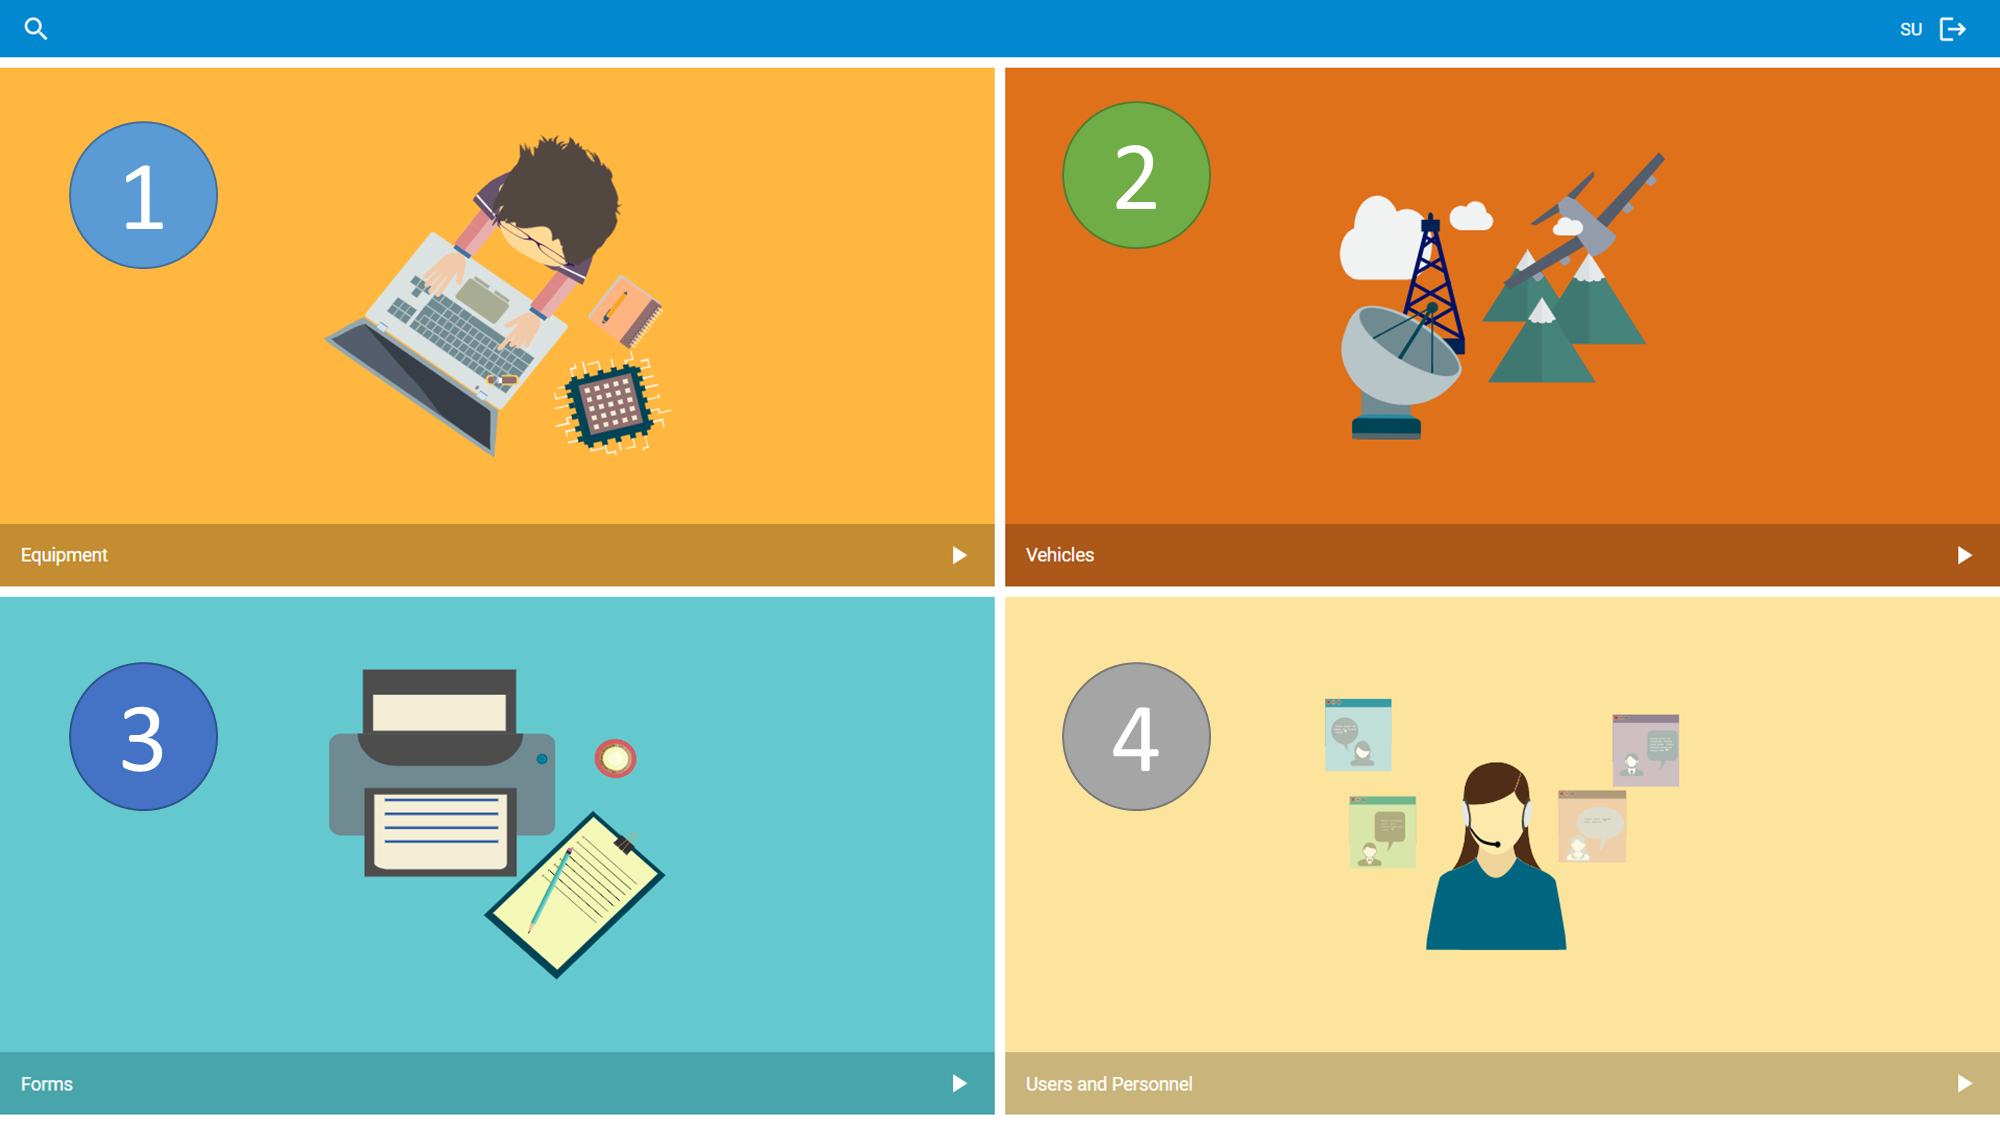
\includegraphics[width=1\textwidth]{sections/00-toc/images/main-menu.png}}
\end{center}

    \clearpage
	
    \setcounter{tocdepth}{3}
    \tableofcontents

    \clearpage

\end{titlepage}

    \pagenumbering{arabic}
    \section{Equipment Module}\label{sec:01}

\subsection{Equipment Class}

In order to perform classification of equipment correctly, users can create equipment classes. Possible equipment classes are hose pipe, ladder, lamp, etc. When creating a new equipment class, users have to fill in its title without white spaces and activity status, as well as its description, as displayed on \hyperref[sections/equipment/images/Fig.1]{Fig.~\ref*{sections/equipment/images/Fig.1}}.

	\begin{figure}[!htbp]
	\centering
	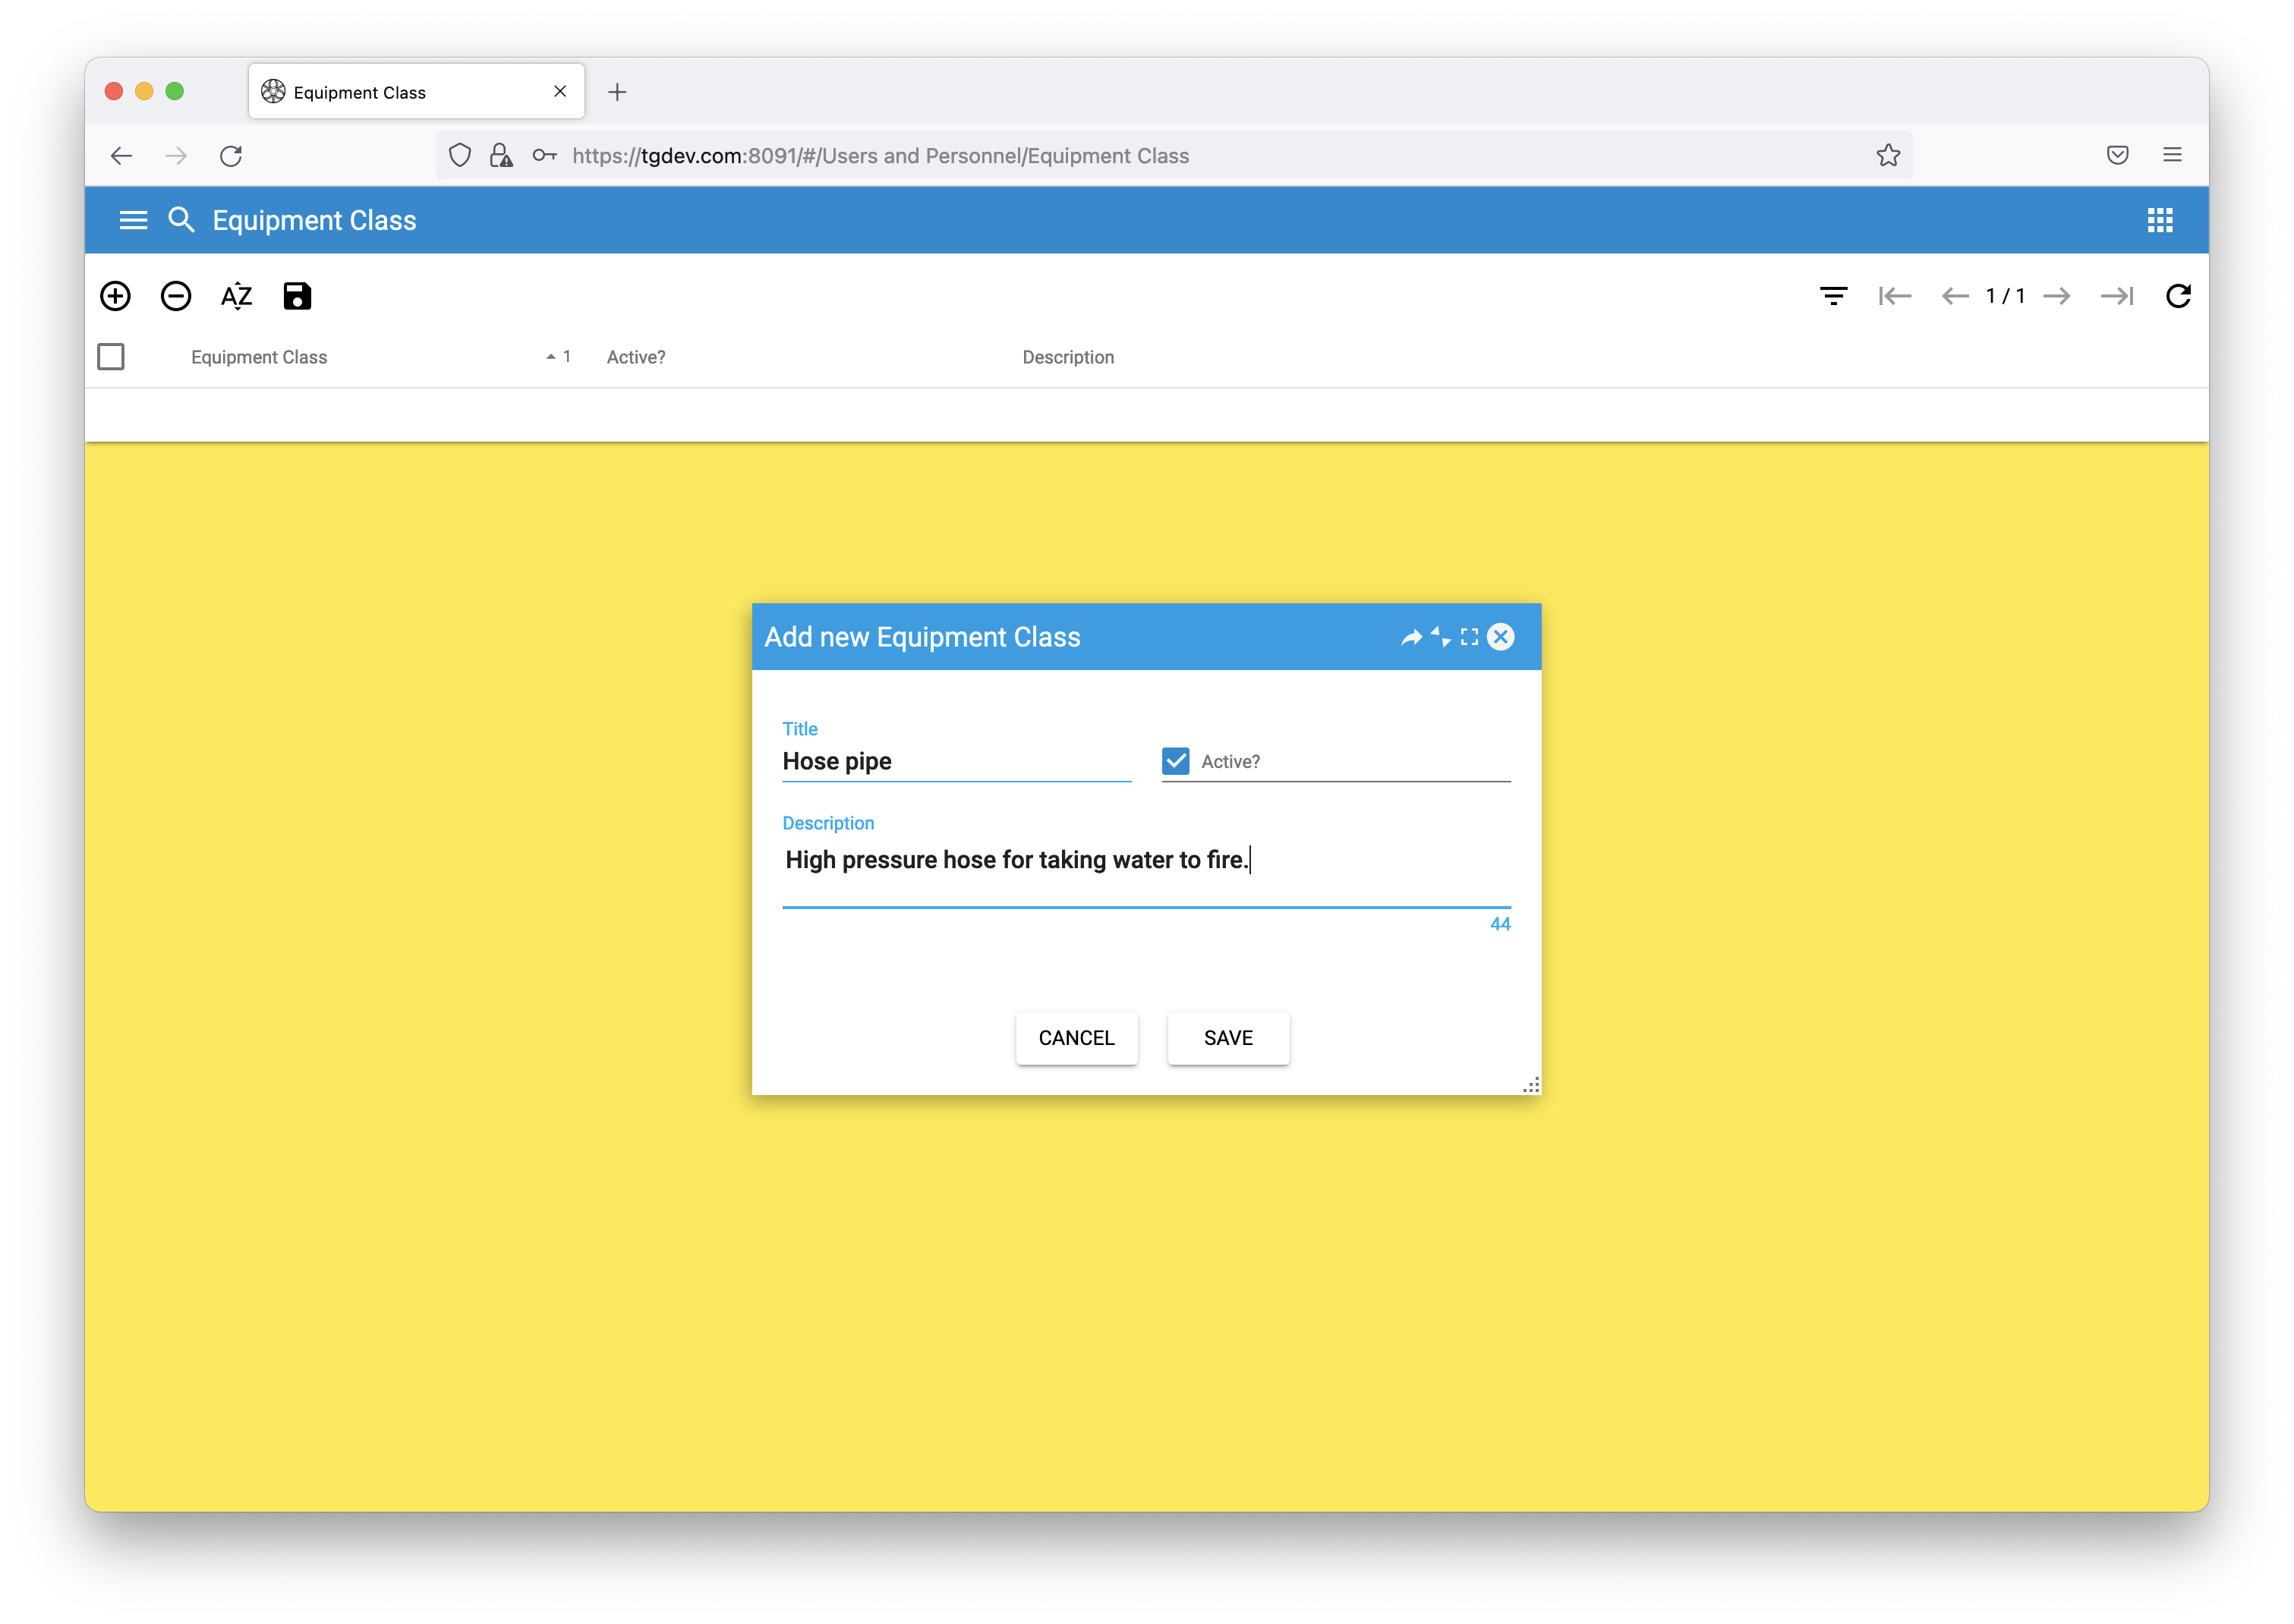
\includegraphics[width=0.95\linewidth]{sections/equipment/images/Fig.1.png}
	\caption{Equipment class creation.}\label{sections/equipment/images/Fig.1}
	\end{figure}
	
Users can search for existing equipment classes either by specifying title, which is auto-completed, or activity status, or both, as displayed on \hyperref[sections/equipment/images/Fig.2]{Fig.~\ref*{sections/equipment/images/Fig.2}}.

    \begin{figure}[!htbp]
	\centering
	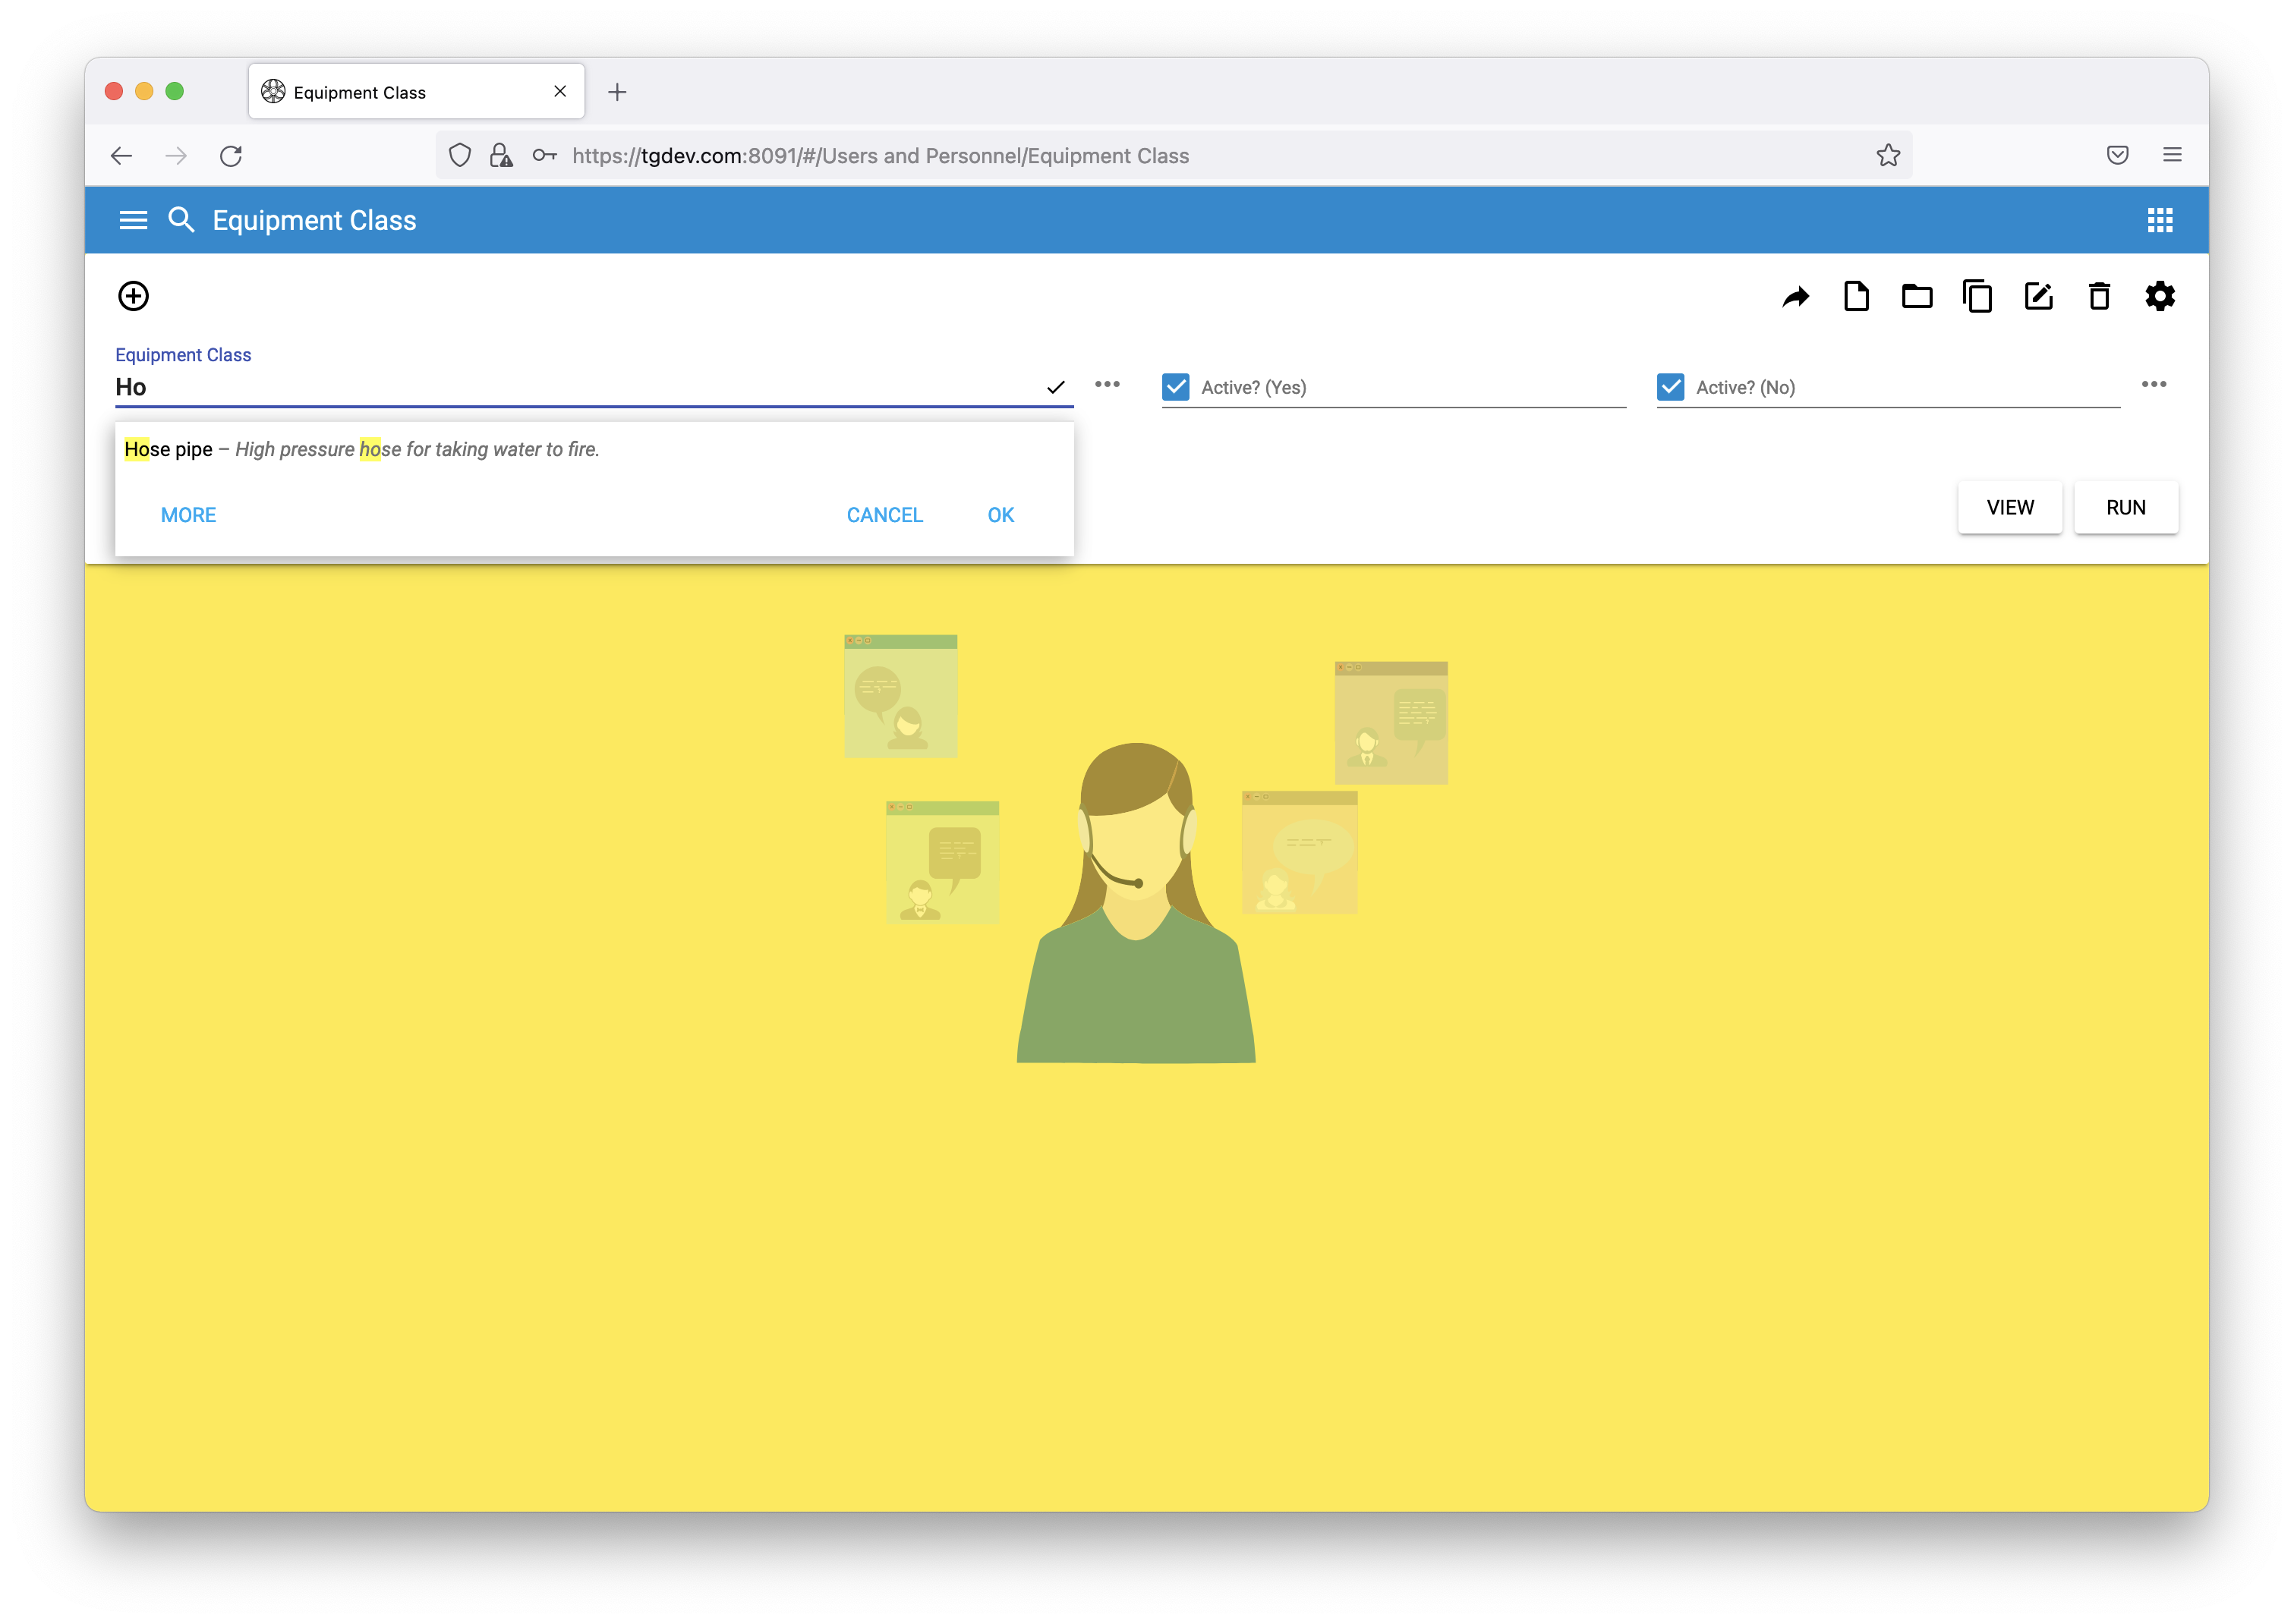
\includegraphics[width=0.95\linewidth]{sections/equipment/images/Fig.2.png}
	\caption{Equipment search query.}\label{sections/equipment/images/Fig.2}
	\end{figure}

\newpage
Search results are displayed along with title, activity status and description of the relevant equipment classes, as displayed on \hyperref[sections/equipment/images/Fig.3]{Fig.~\ref*{sections/equipment/images/Fig.3}}.

    \begin{figure}[!htbp]
	\centering
	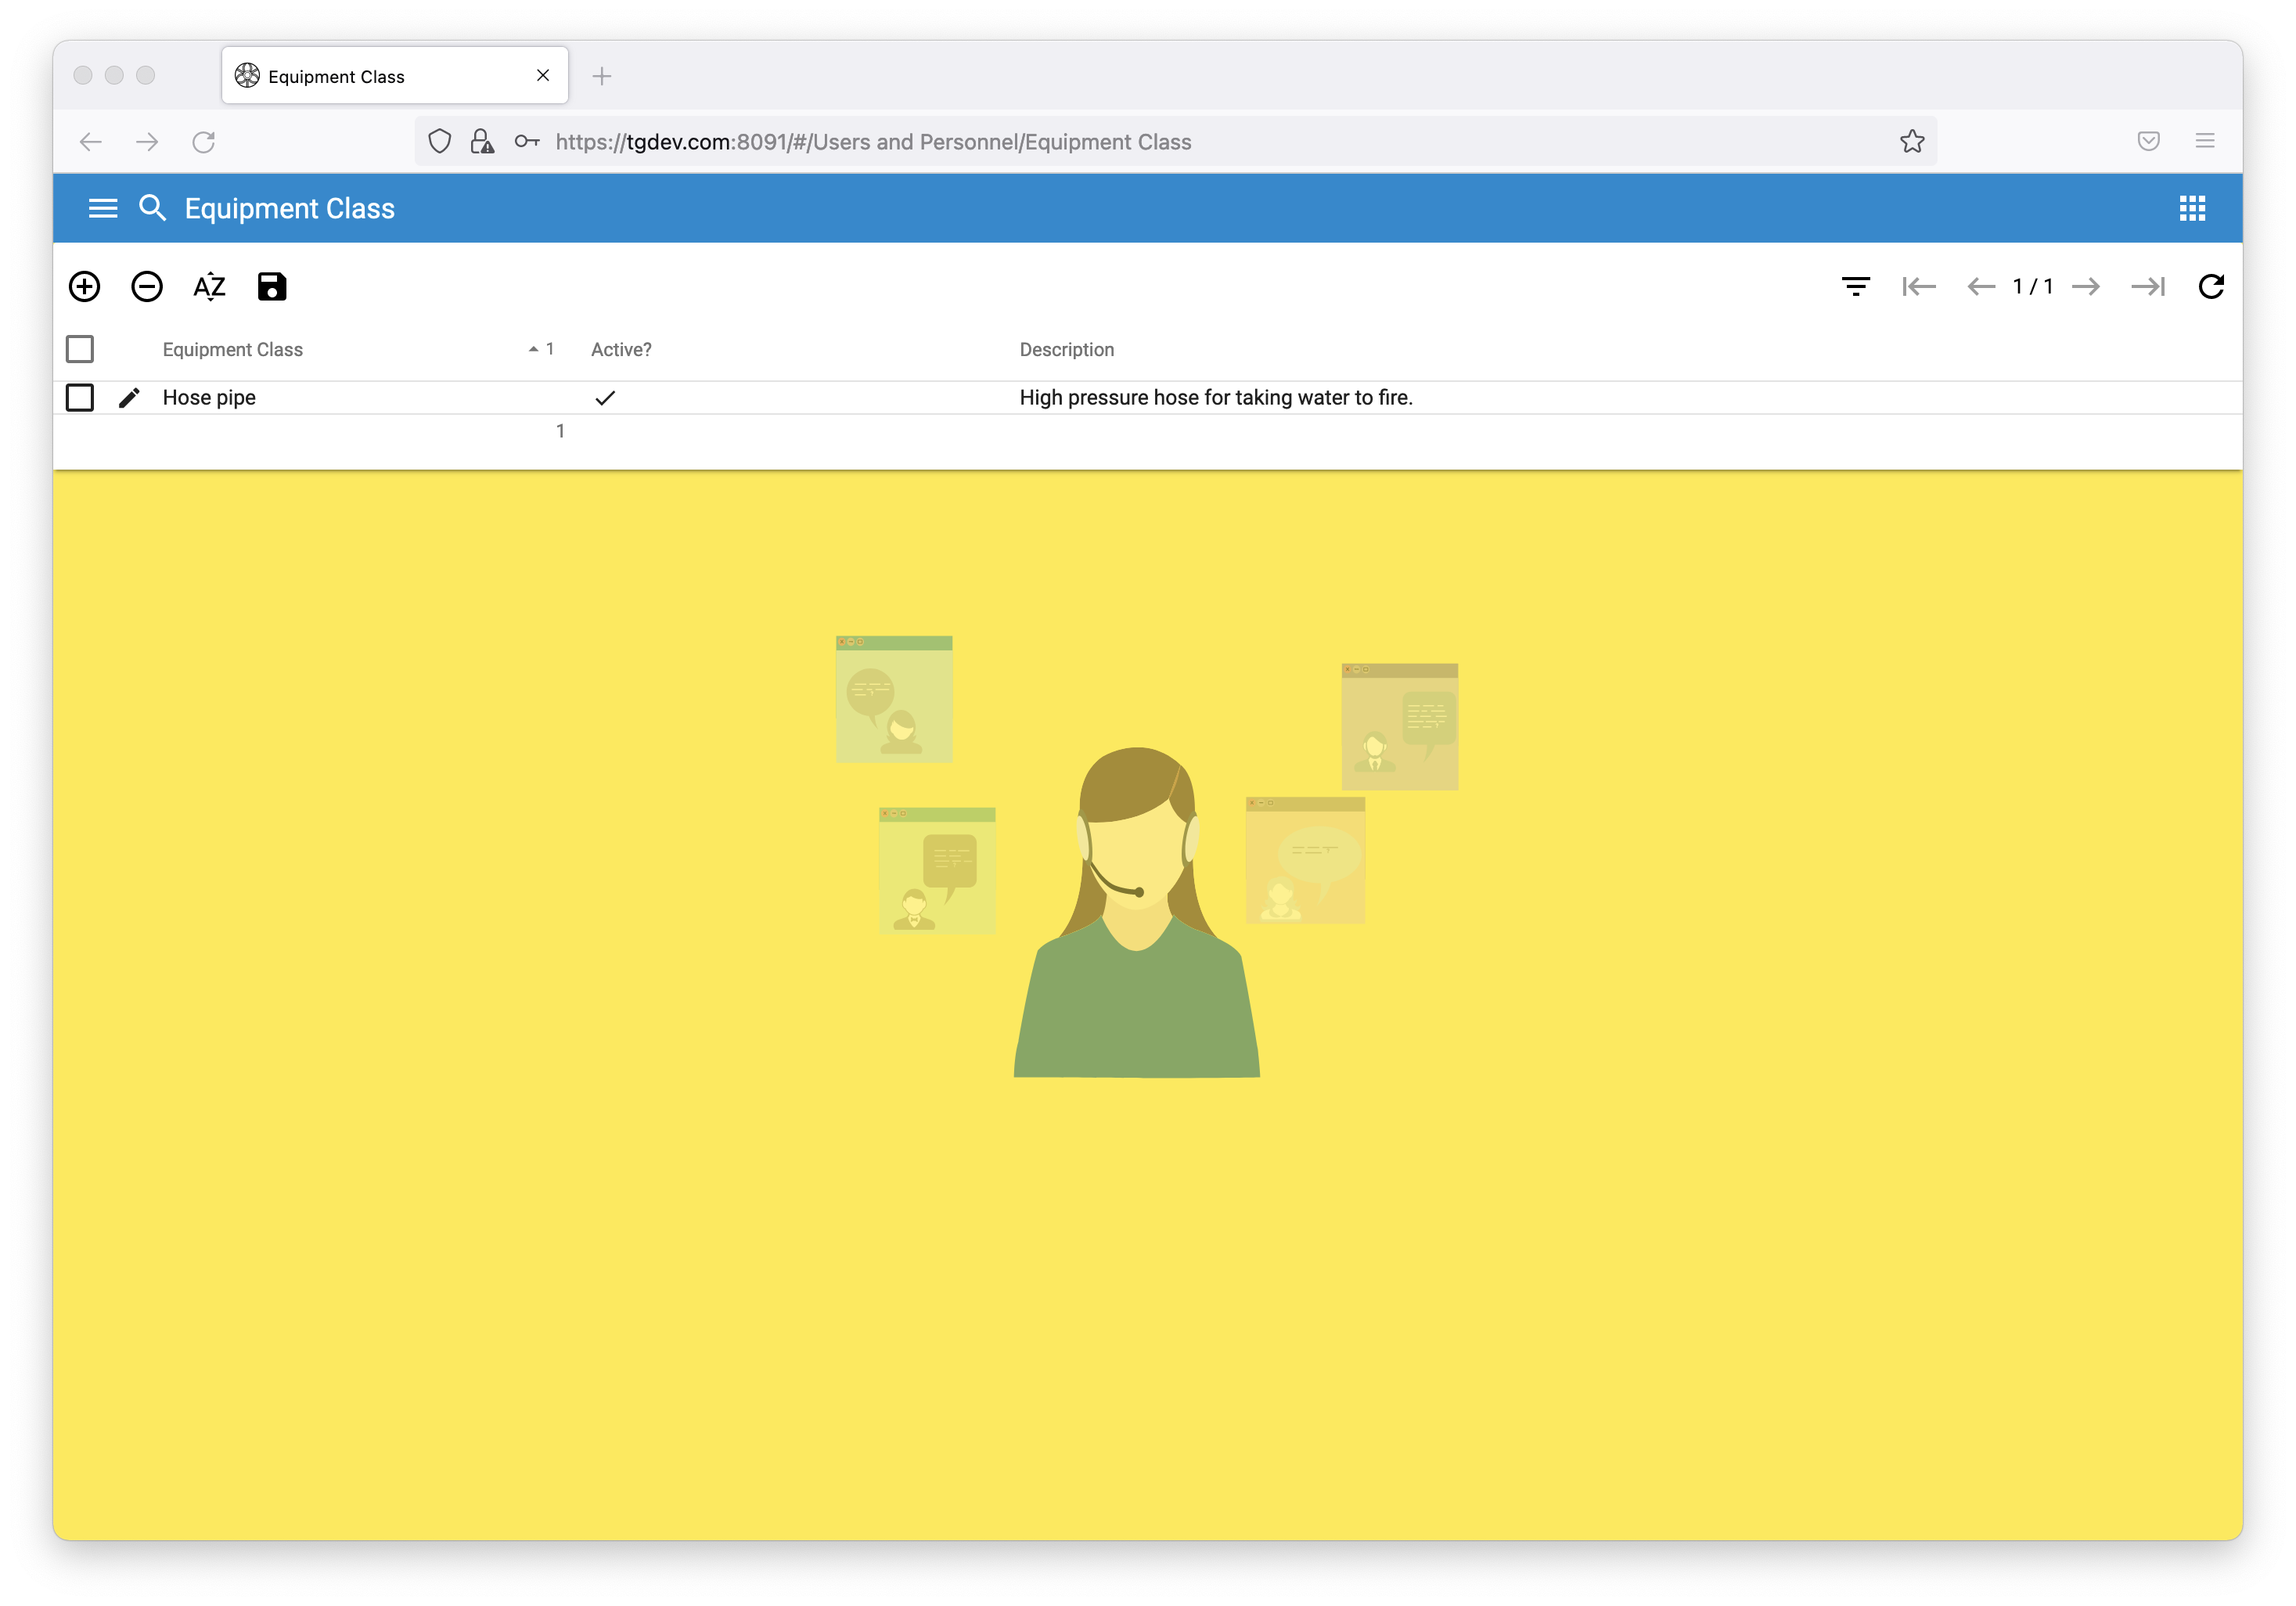
\includegraphics[width=0.95\linewidth]{sections/equipment/images/Fig.3.png}
	\caption{Equipment class search results.}\label{sections/equipment/images/Fig.3}
	\end{figure}
	
\newpage
Users can edit existing equipment classes. On the 'Main' tab, displayed on \hyperref[sections/equipment/images/Fig.4]{Fig.~\ref*{sections/equipment/images/Fig.4}}, users can edit title, activity status and description of the specific equipment class.

    \begin{figure}[!htbp]
	\centering
	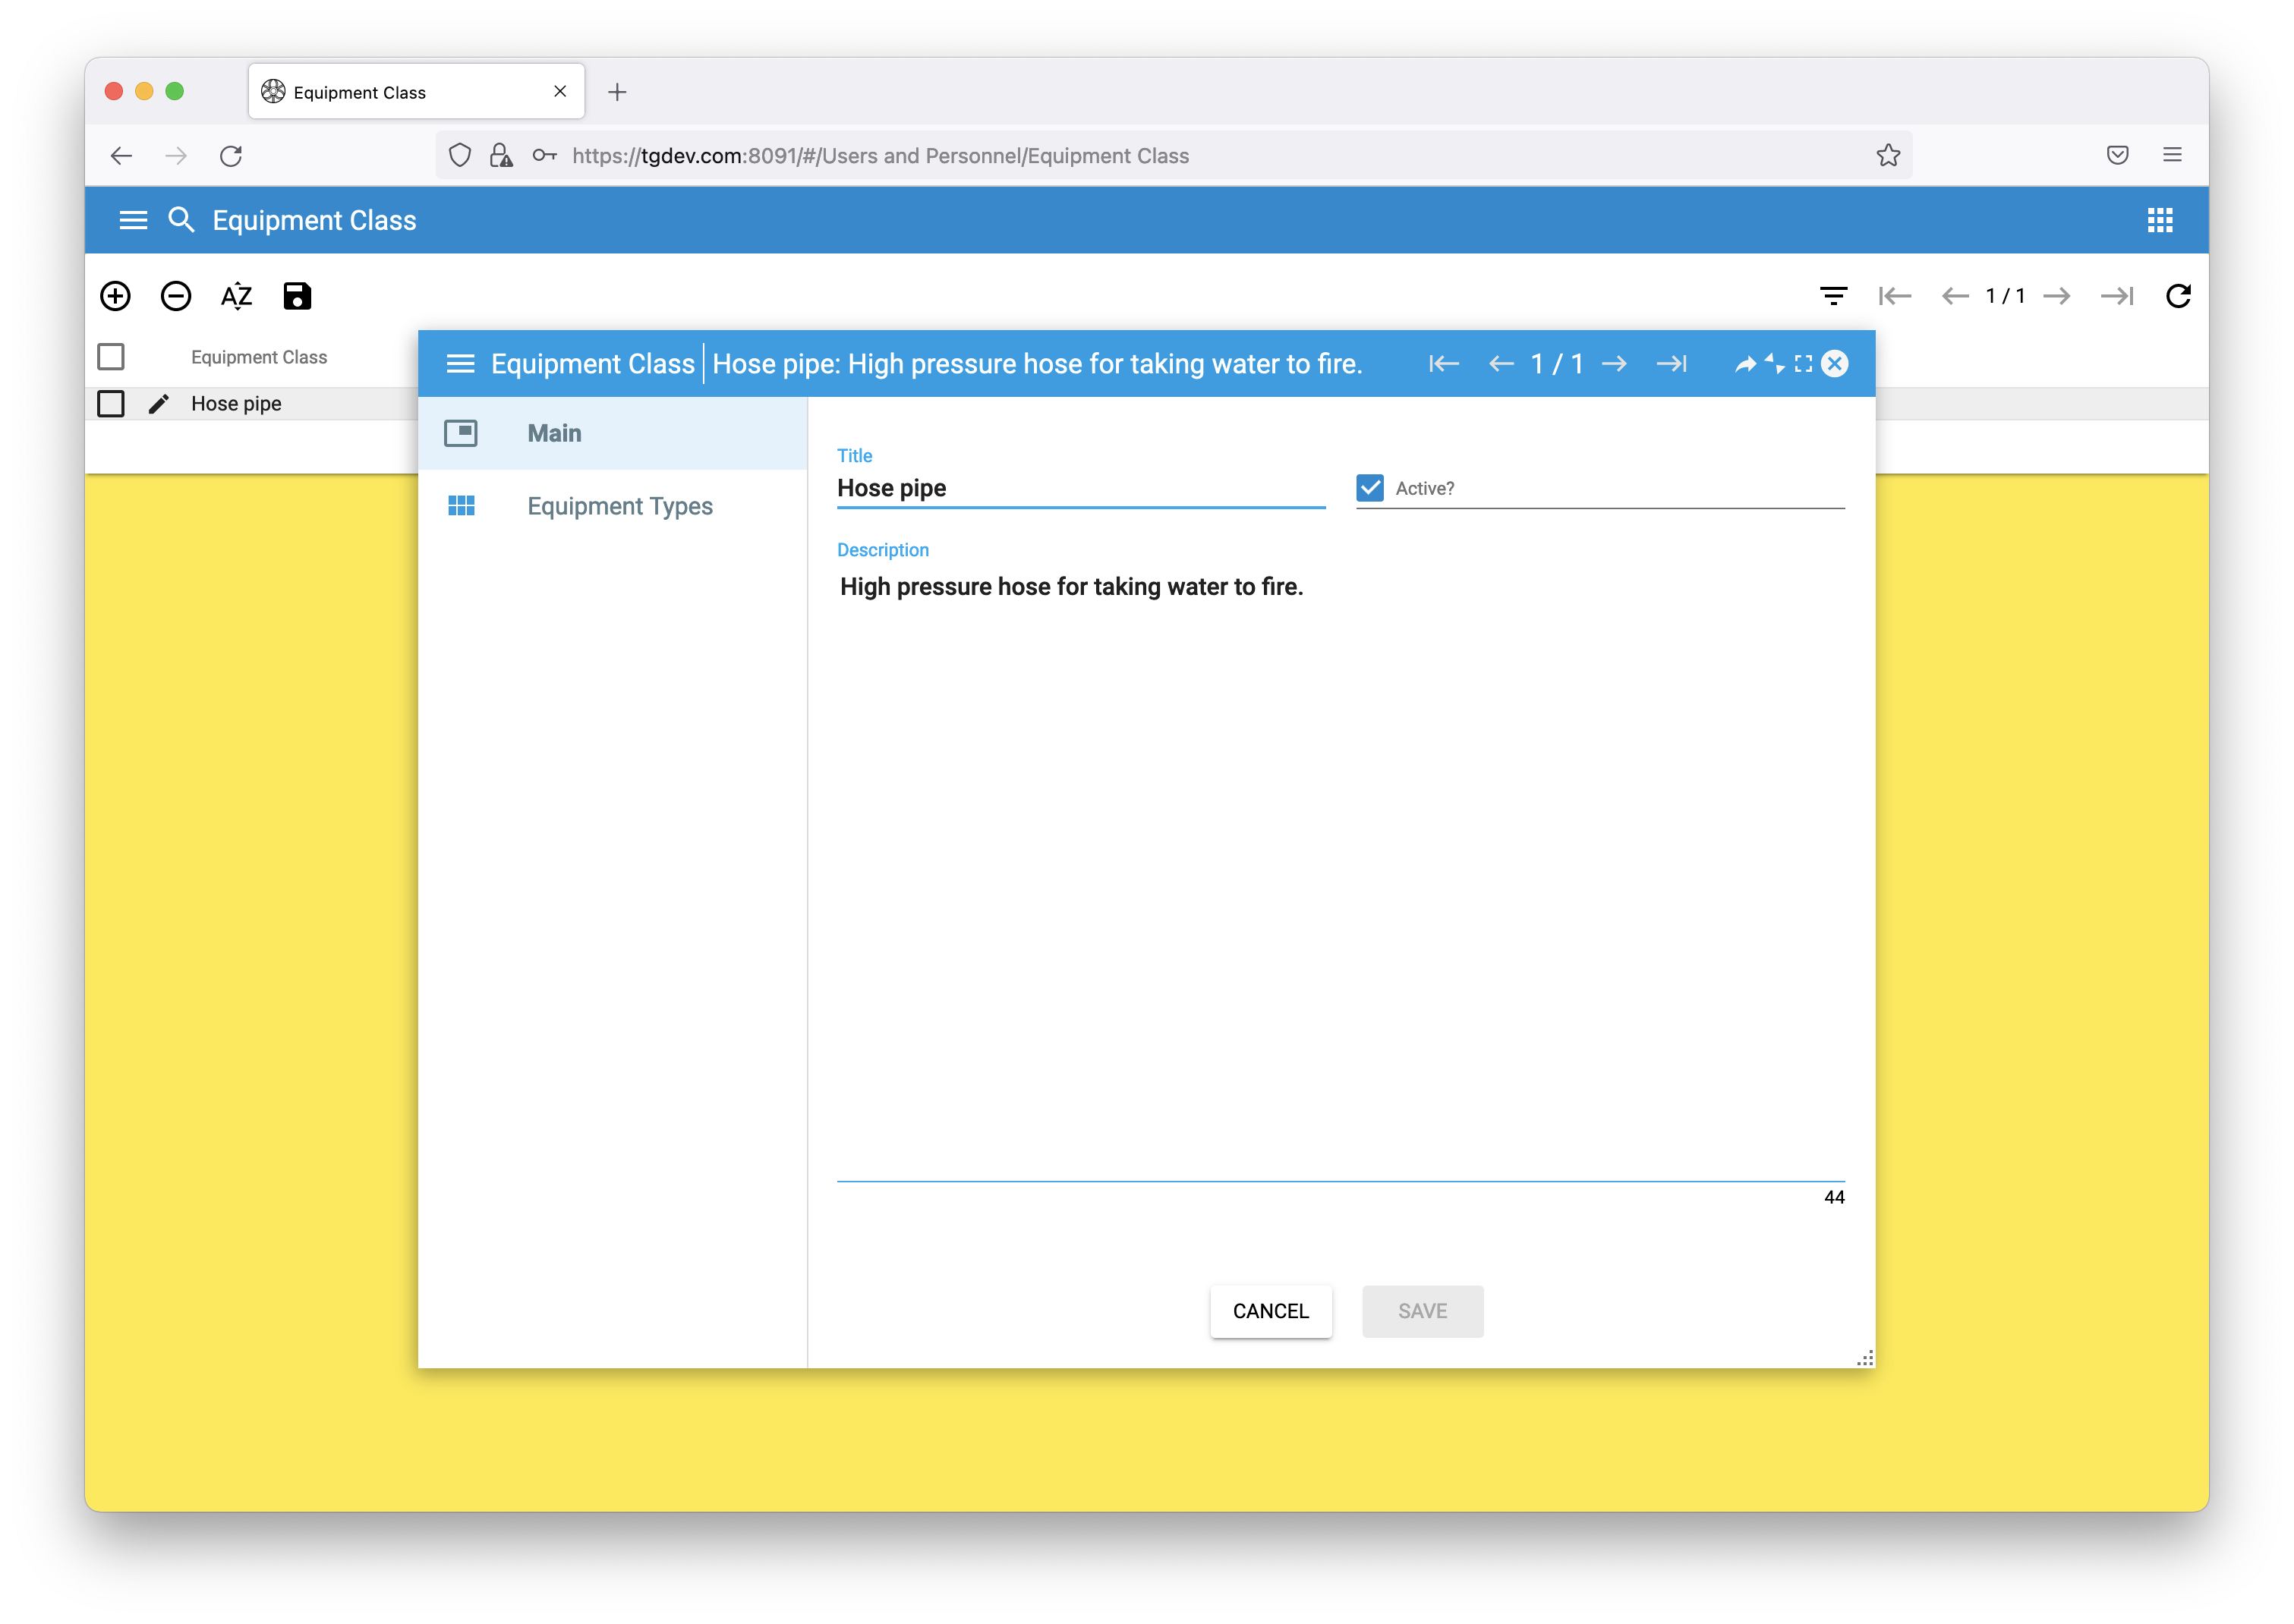
\includegraphics[width=0.95\linewidth]{sections/equipment/images/Fig.4.png}
	\caption{Equipment class editing.}\label{sections/equipment/images/Fig.4}
	\end{figure}

\newpage
On the ‘Equipment Types’ tab, users can:
\begin{itemize}
    \item observe all of the equipment types related only to this specific equipment class along with title, activity status and description, as displayed on \hyperref[sections/equipment/images/Fig.5]{Fig.~\ref*{sections/equipment/images/Fig.5}};
\end{itemize}

    \begin{figure}[!htbp]
	\centering
	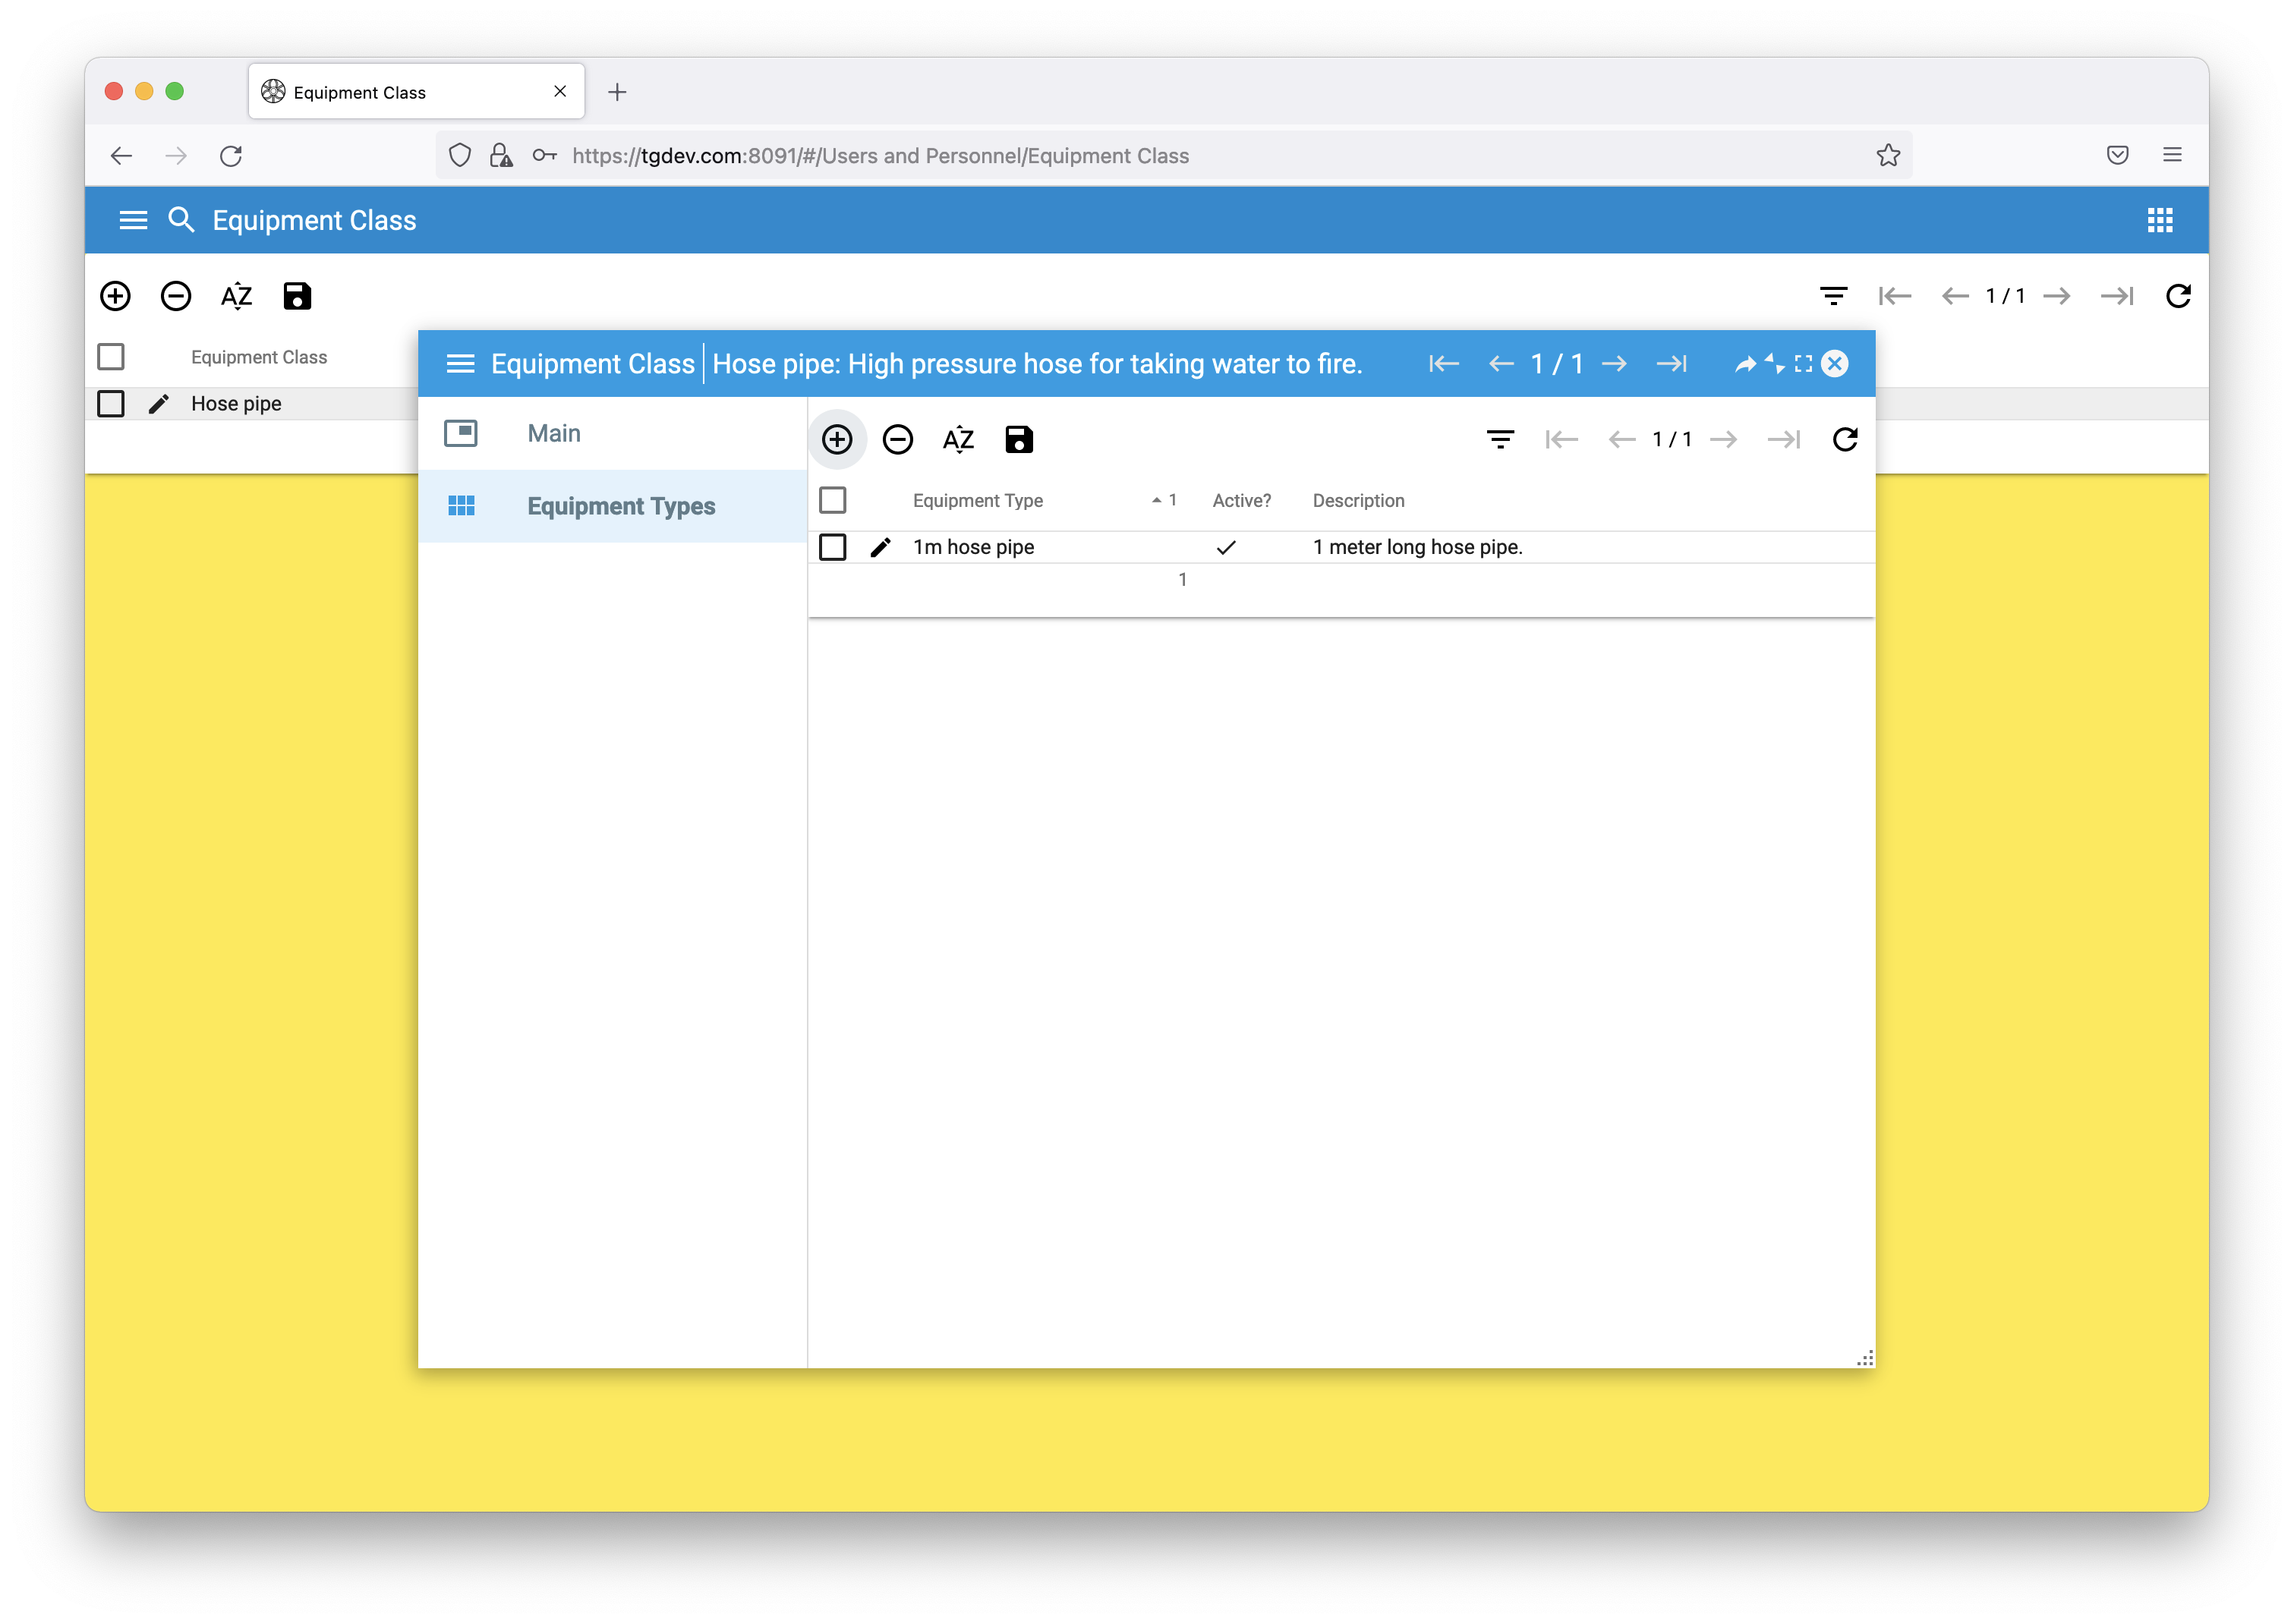
\includegraphics[width=0.95\linewidth]{sections/equipment/images/Fig.5.png}
	\caption{Embedded equipment type search results.}\label{sections/equipment/images/Fig.5}
	\end{figure}
	
\newpage
\begin{itemize}
    \item search for existing equipment types related only to this specific equipment class either by specifying title, which is auto-completed, or activity status, or both, as displayed on \hyperref[sections/equipment/images/Fig.6]{Fig.~\ref*{sections/equipment/images/Fig.6}};
\end{itemize}

    \begin{figure}[!htbp]
	\centering
	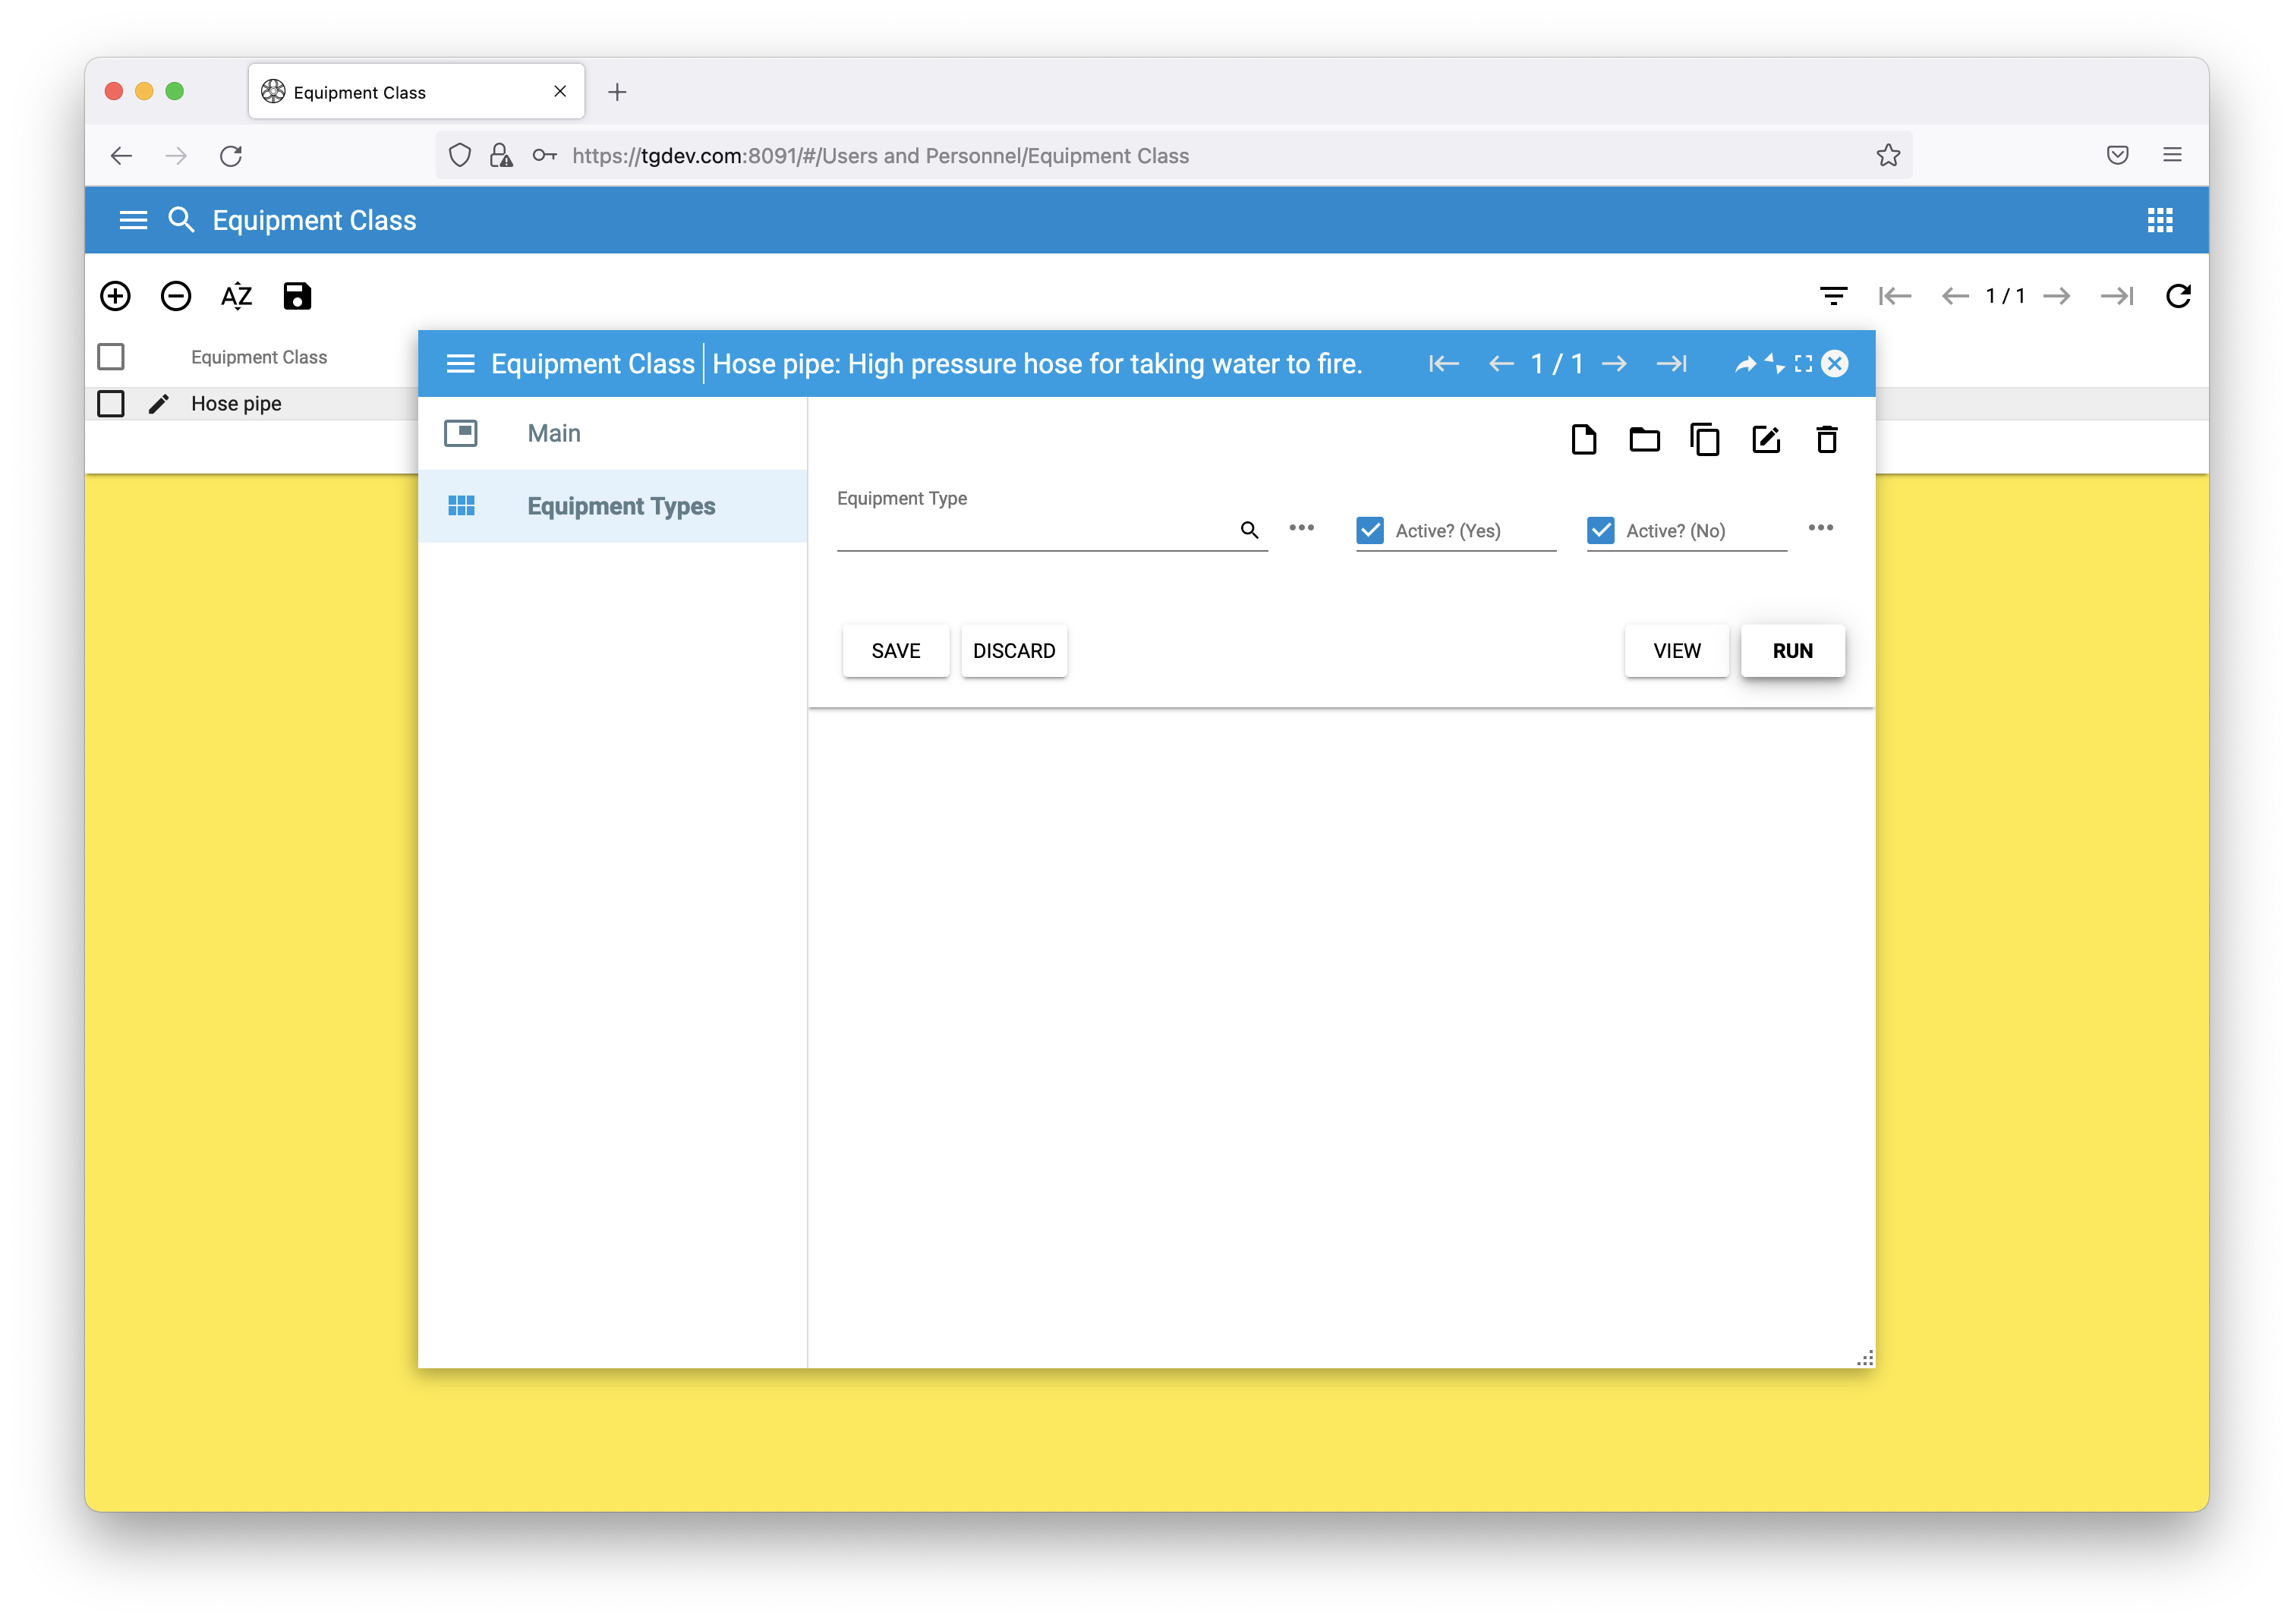
\includegraphics[width=0.95\linewidth]{sections/equipment/images/Fig.6.png}
	\caption{Embedded equipment type search query.}\label{sections/equipment/images/Fig.6}
	\end{figure}
	
\newpage
\begin{itemize}
    \item create equipment type by filling in its title without white spaces and activity status, as well as its description, as displayed on \hyperref[sections/equipment/images/Fig.7]{Fig.~\ref*{sections/equipment/images/Fig.7}}. Equipment class field is automatically auto-completed with this specific equipment class.
\end{itemize}

    \begin{figure}[!htbp]
	\centering
	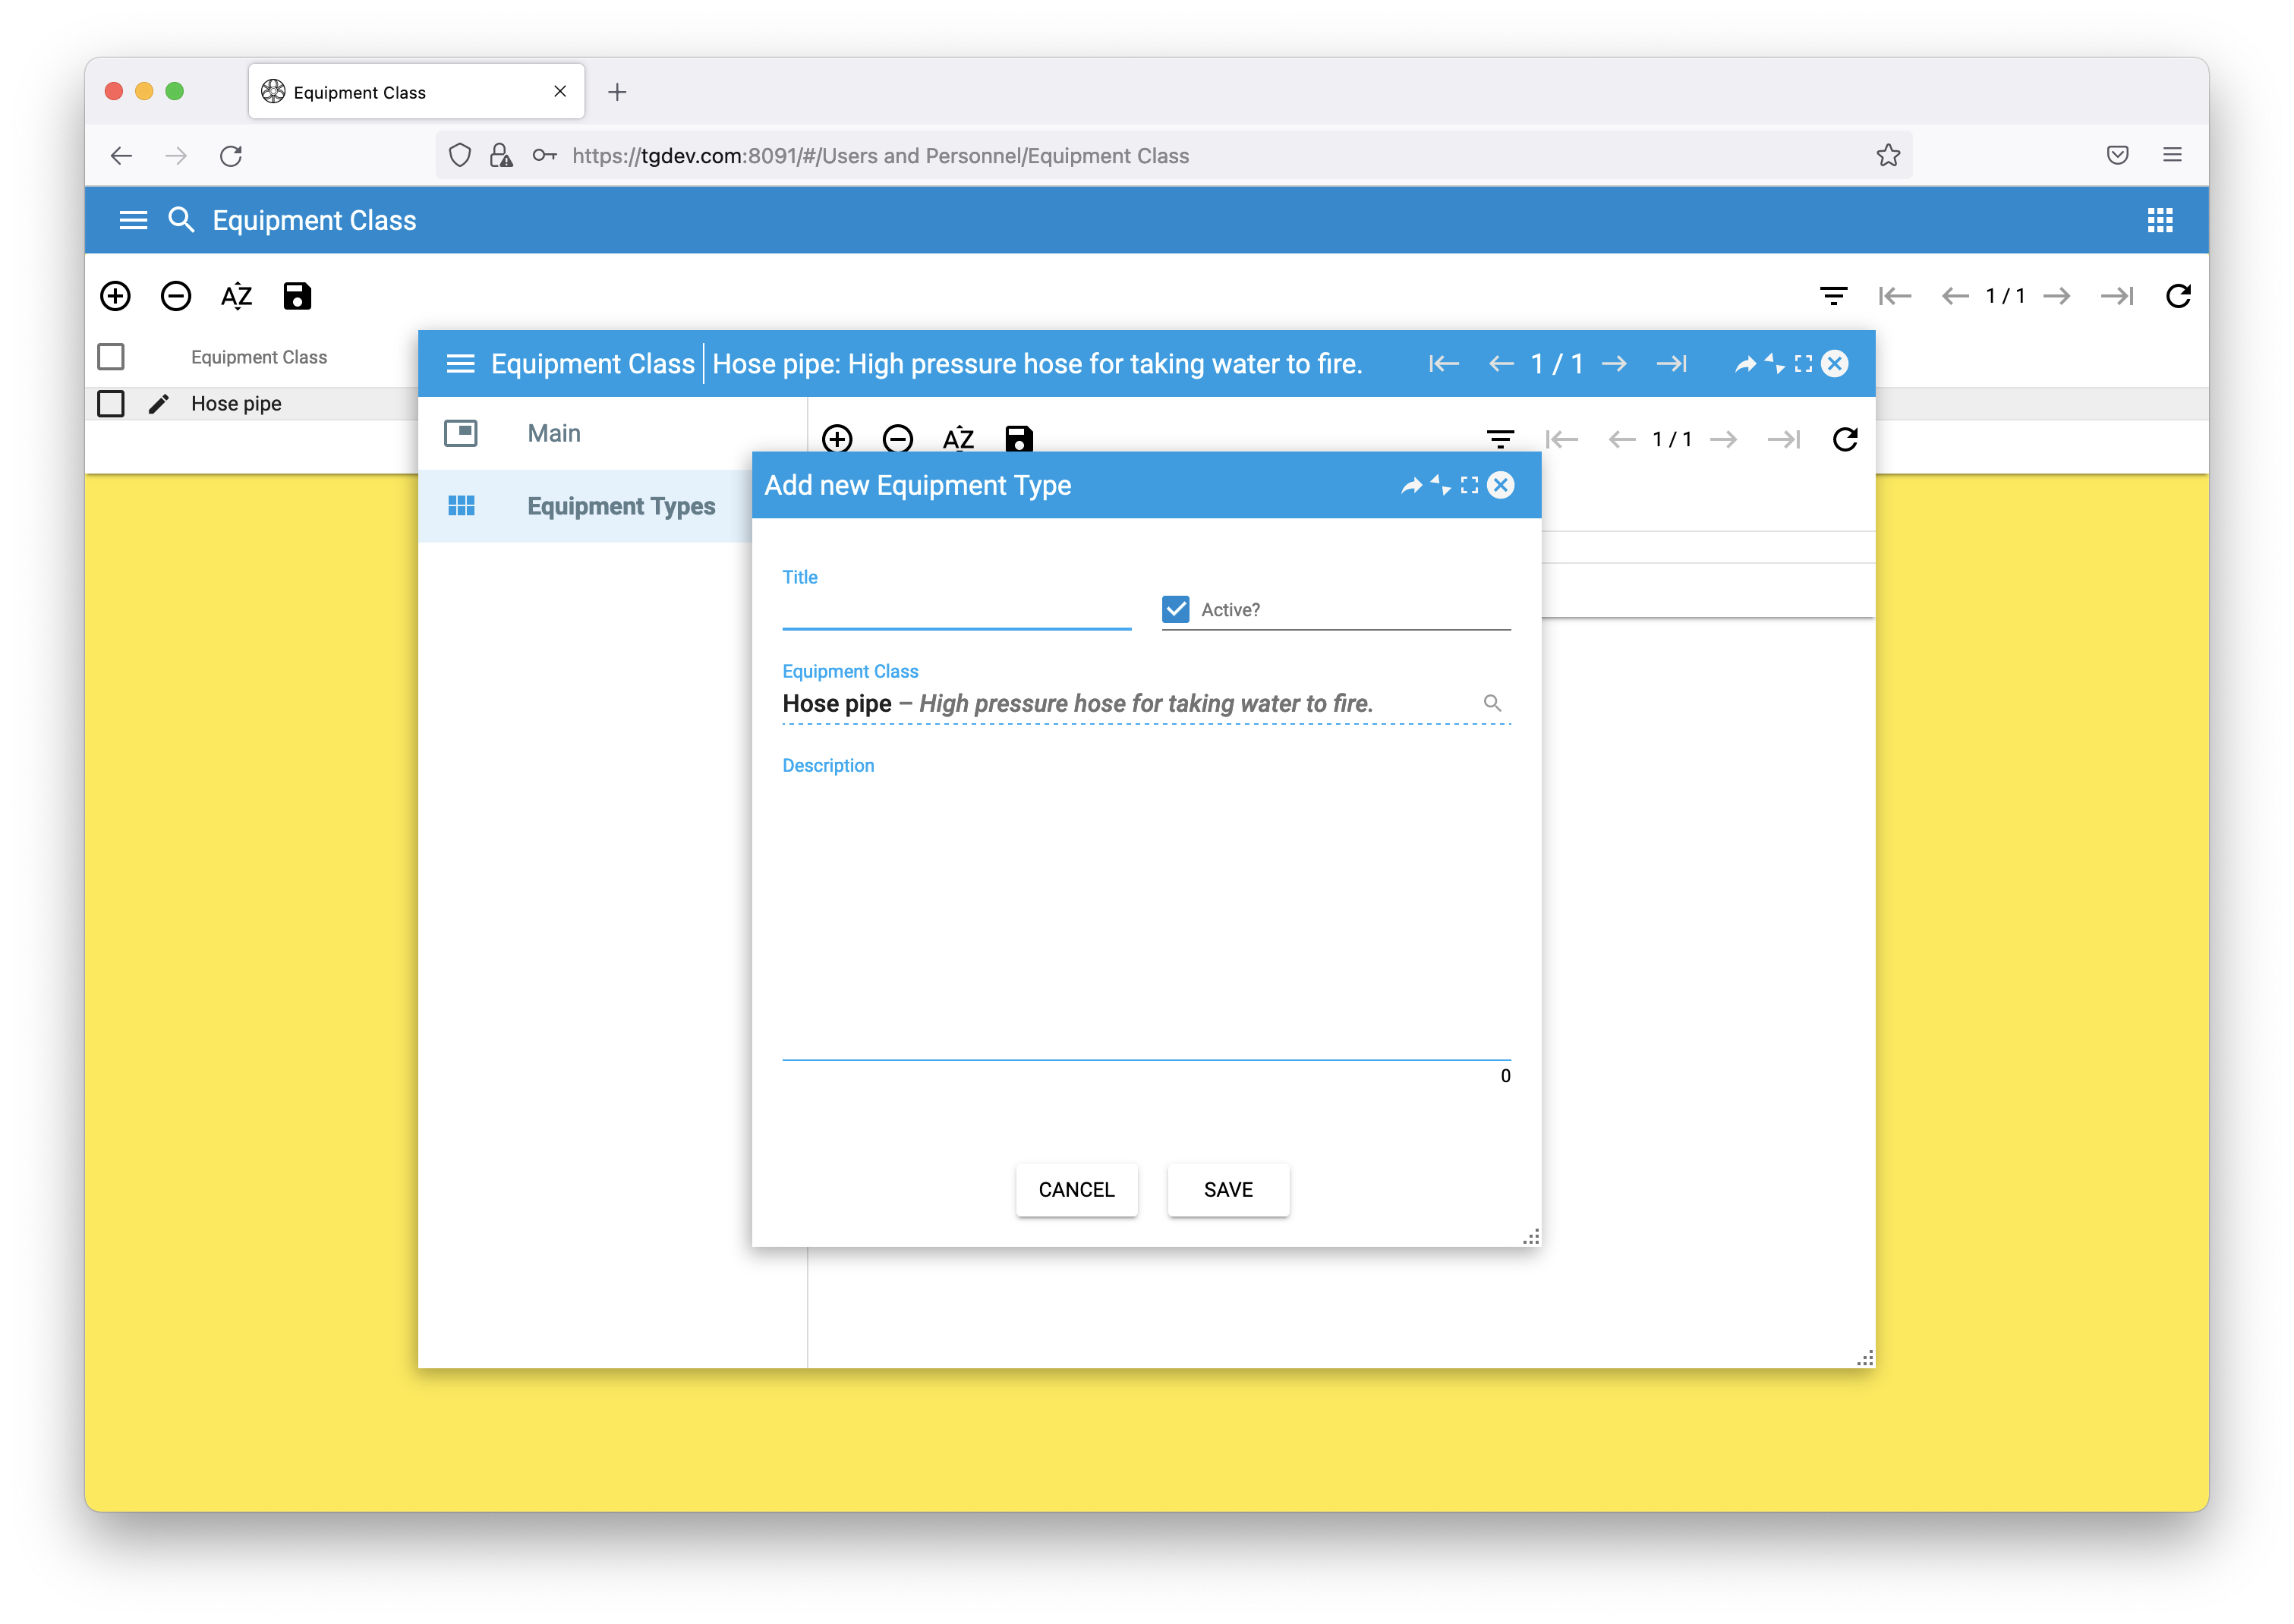
\includegraphics[width=0.95\linewidth]{sections/equipment/images/Fig.7.png}
	\caption{Embedded equipment type creation.}\label{sections/equipment/images/Fig.7}
	\end{figure}

\newpage	
\subsection{Equipment Type}

In order to perform classification of equipment in more detail correctly, users can create equipment types. Possible equipment types are 1m hose pipe, assault ladder, electric lamp, etc. When creating a new equipment type, users have to fill in its title without white spaces, activity status, equipment class it belongs to, which is auto-completed, as well as its description, as displayed on \hyperref[sections/equipment/images/Fig.8]{Fig.~\ref*{sections/equipment/images/Fig.8}}. 

    \begin{figure}[!htbp]
	\centering
	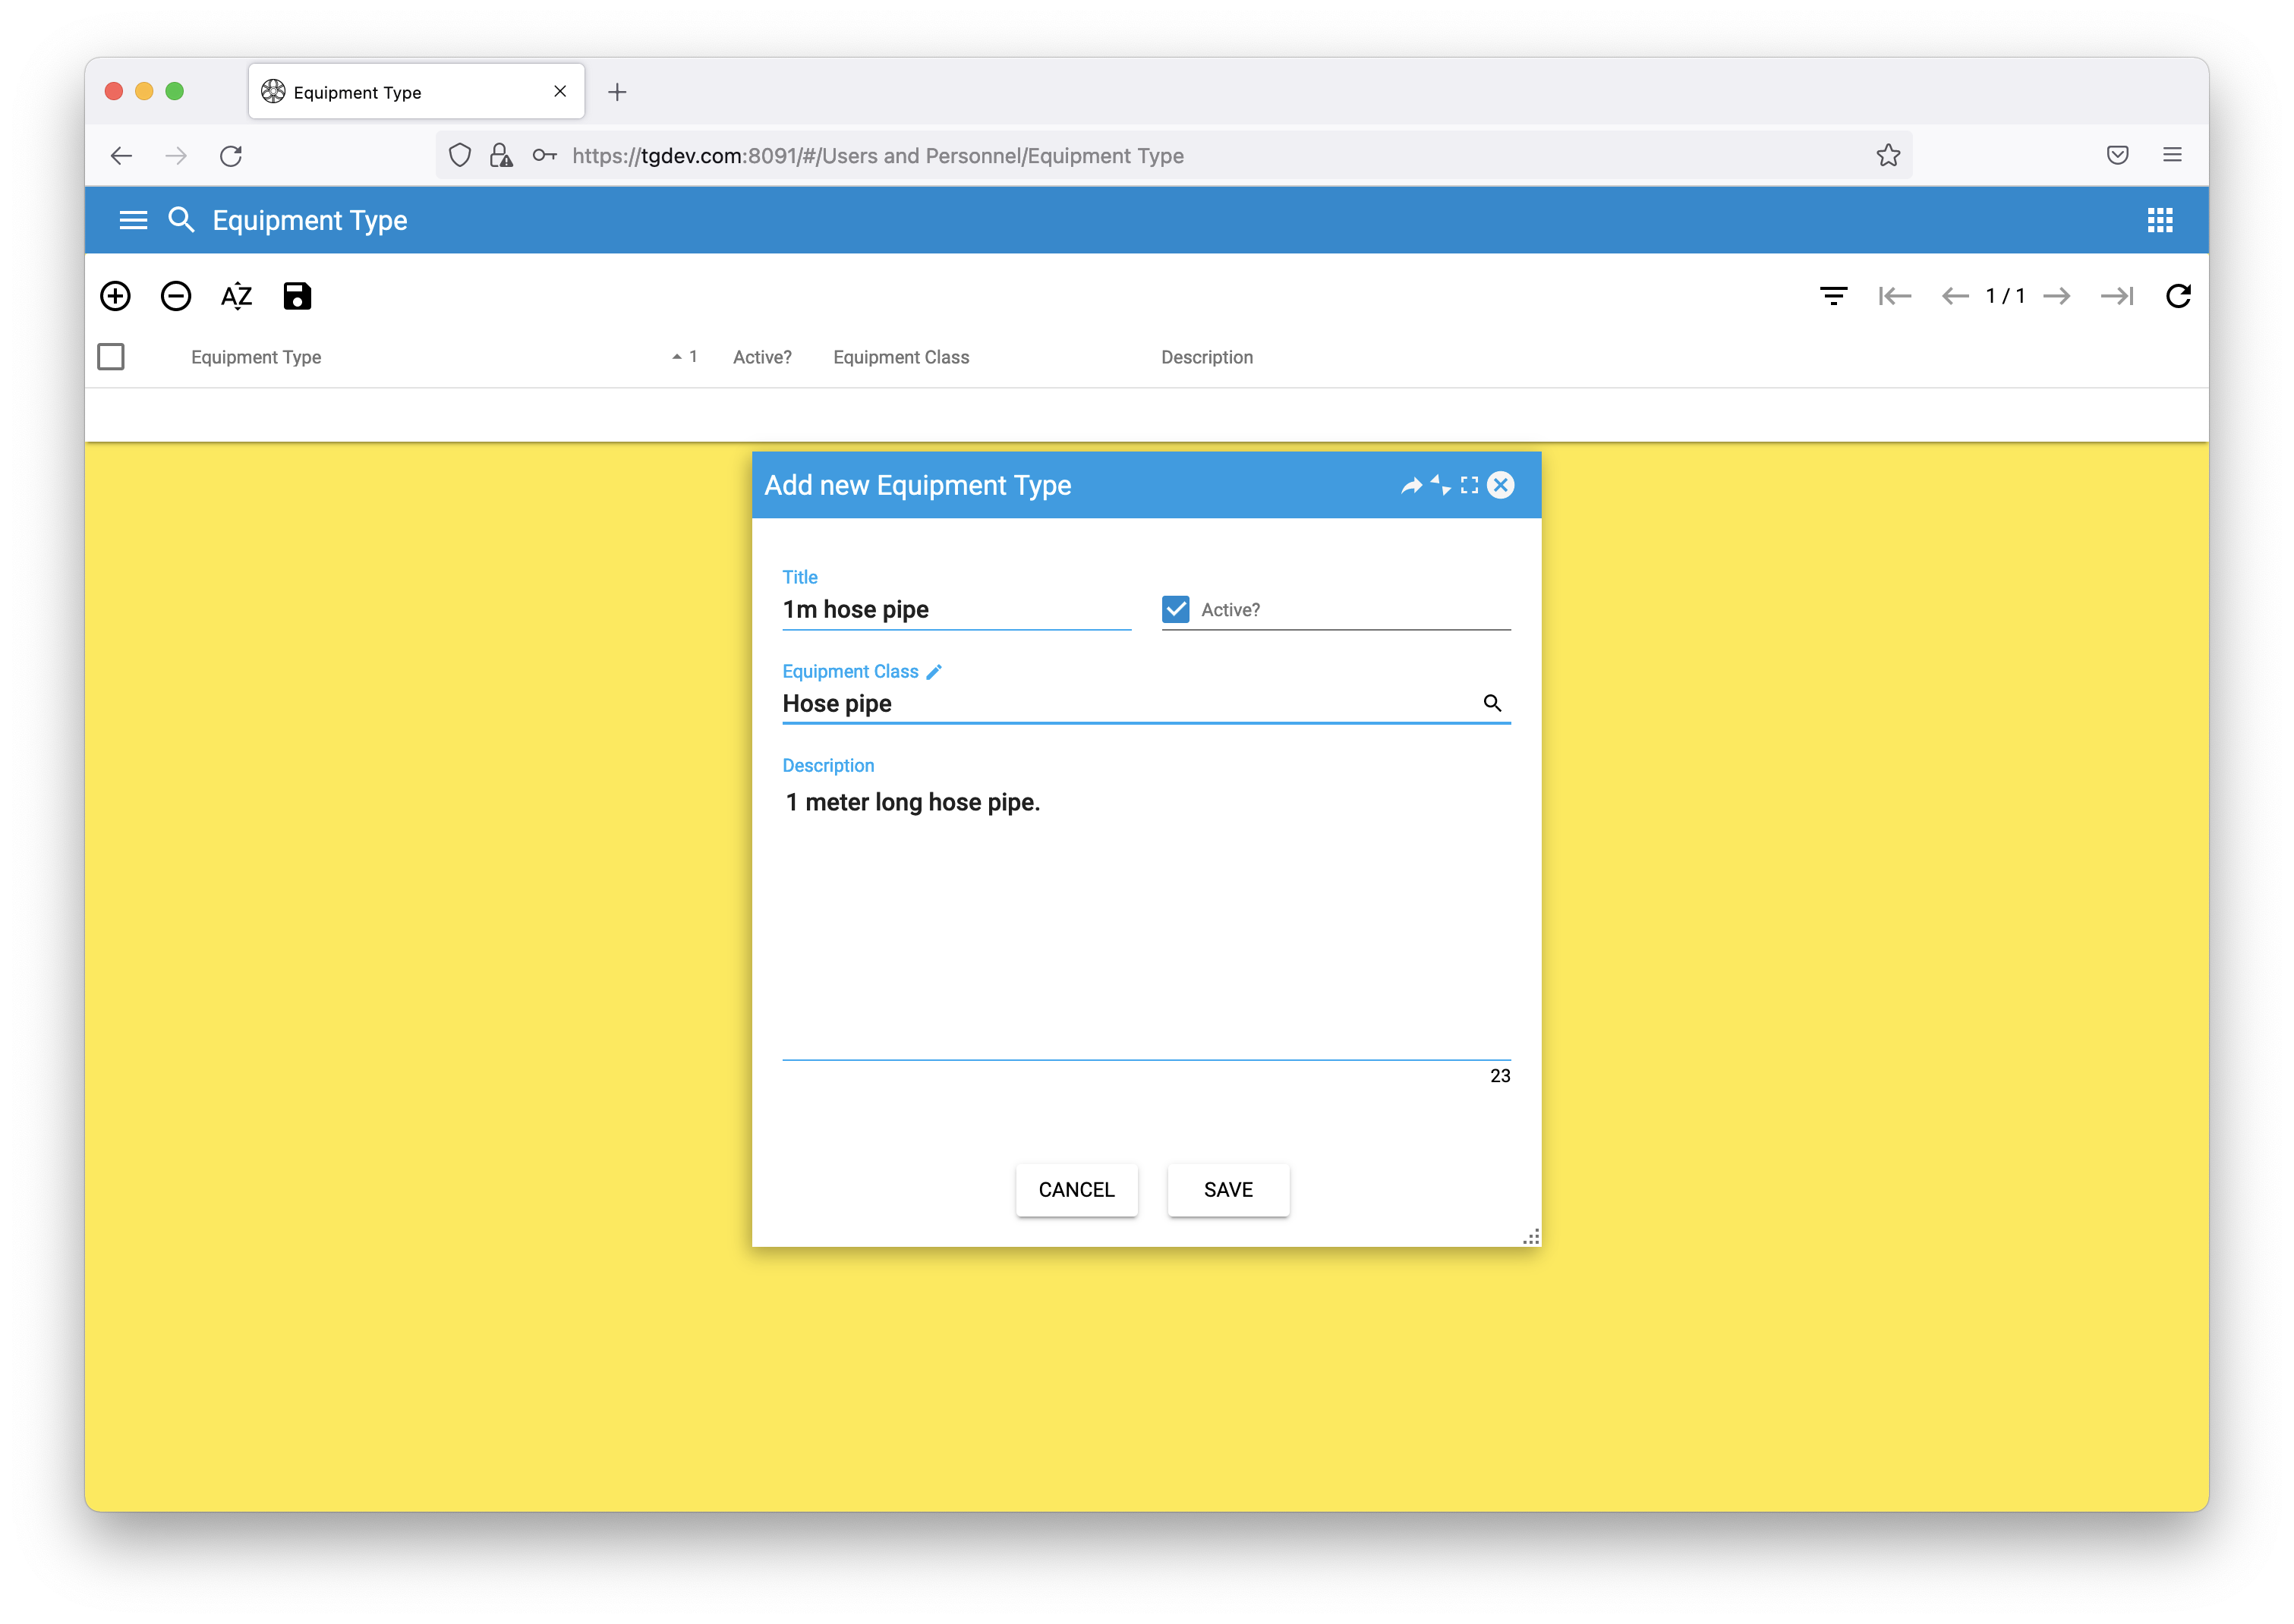
\includegraphics[width=0.95\linewidth]{sections/equipment/images/Fig.8.png}
	\caption{Equipment type creation.}\label{sections/equipment/images/Fig.8}
	\end{figure}

\newpage
Users can search for existing equipment types either by specifying title, which is auto-completed, activity status, equipment class they belong to, or all, as displayed on \hyperref[sections/equipment/images/Fig.9]{Fig.~\ref*{sections/equipment/images/Fig.9}}.

    \begin{figure}[!htbp]
	\centering
	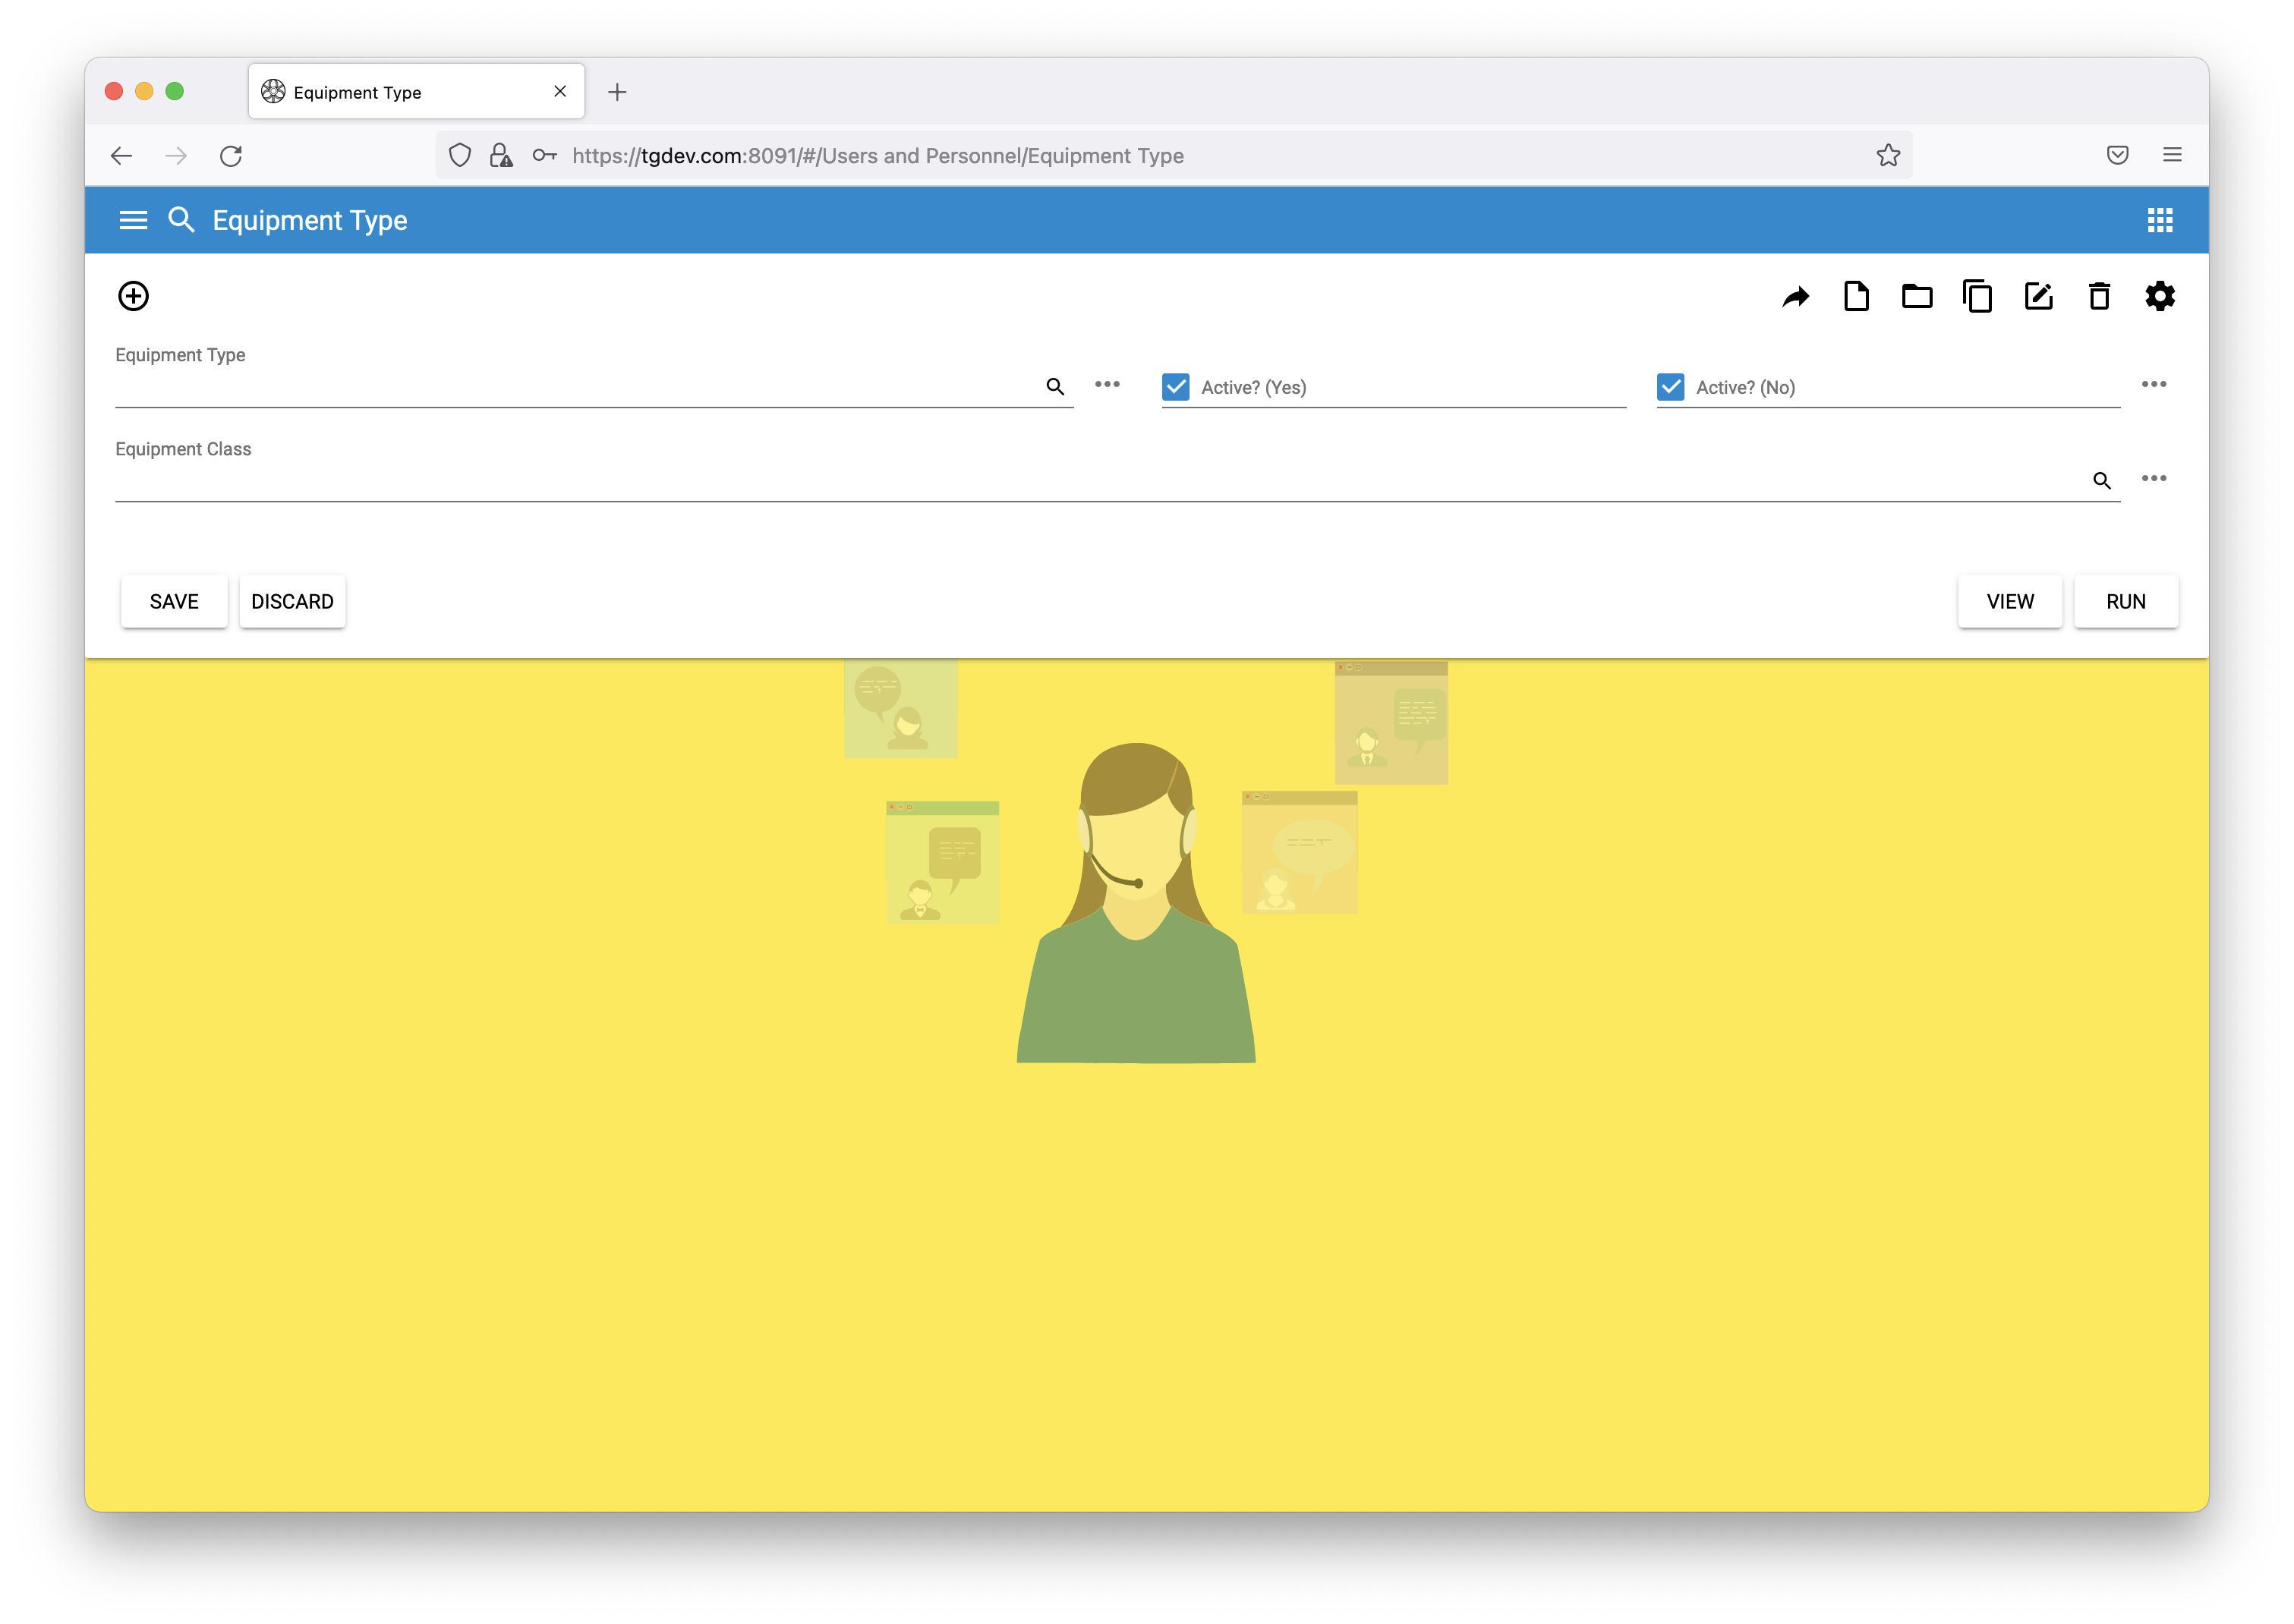
\includegraphics[width=0.95\linewidth]{sections/equipment/images/Fig.9.png}
	\caption{Equipment type search query.}\label{sections/equipment/images/Fig.9}
	\end{figure}
	
\newpage
Search results are displayed along with title, activity status, equipment class and description of the equipment type, as displayed on \hyperref[sections/equipment/images/Fig.10]{Fig.~\ref*{sections/equipment/images/Fig.10}}.

    \begin{figure}[!htbp]
	\centering
	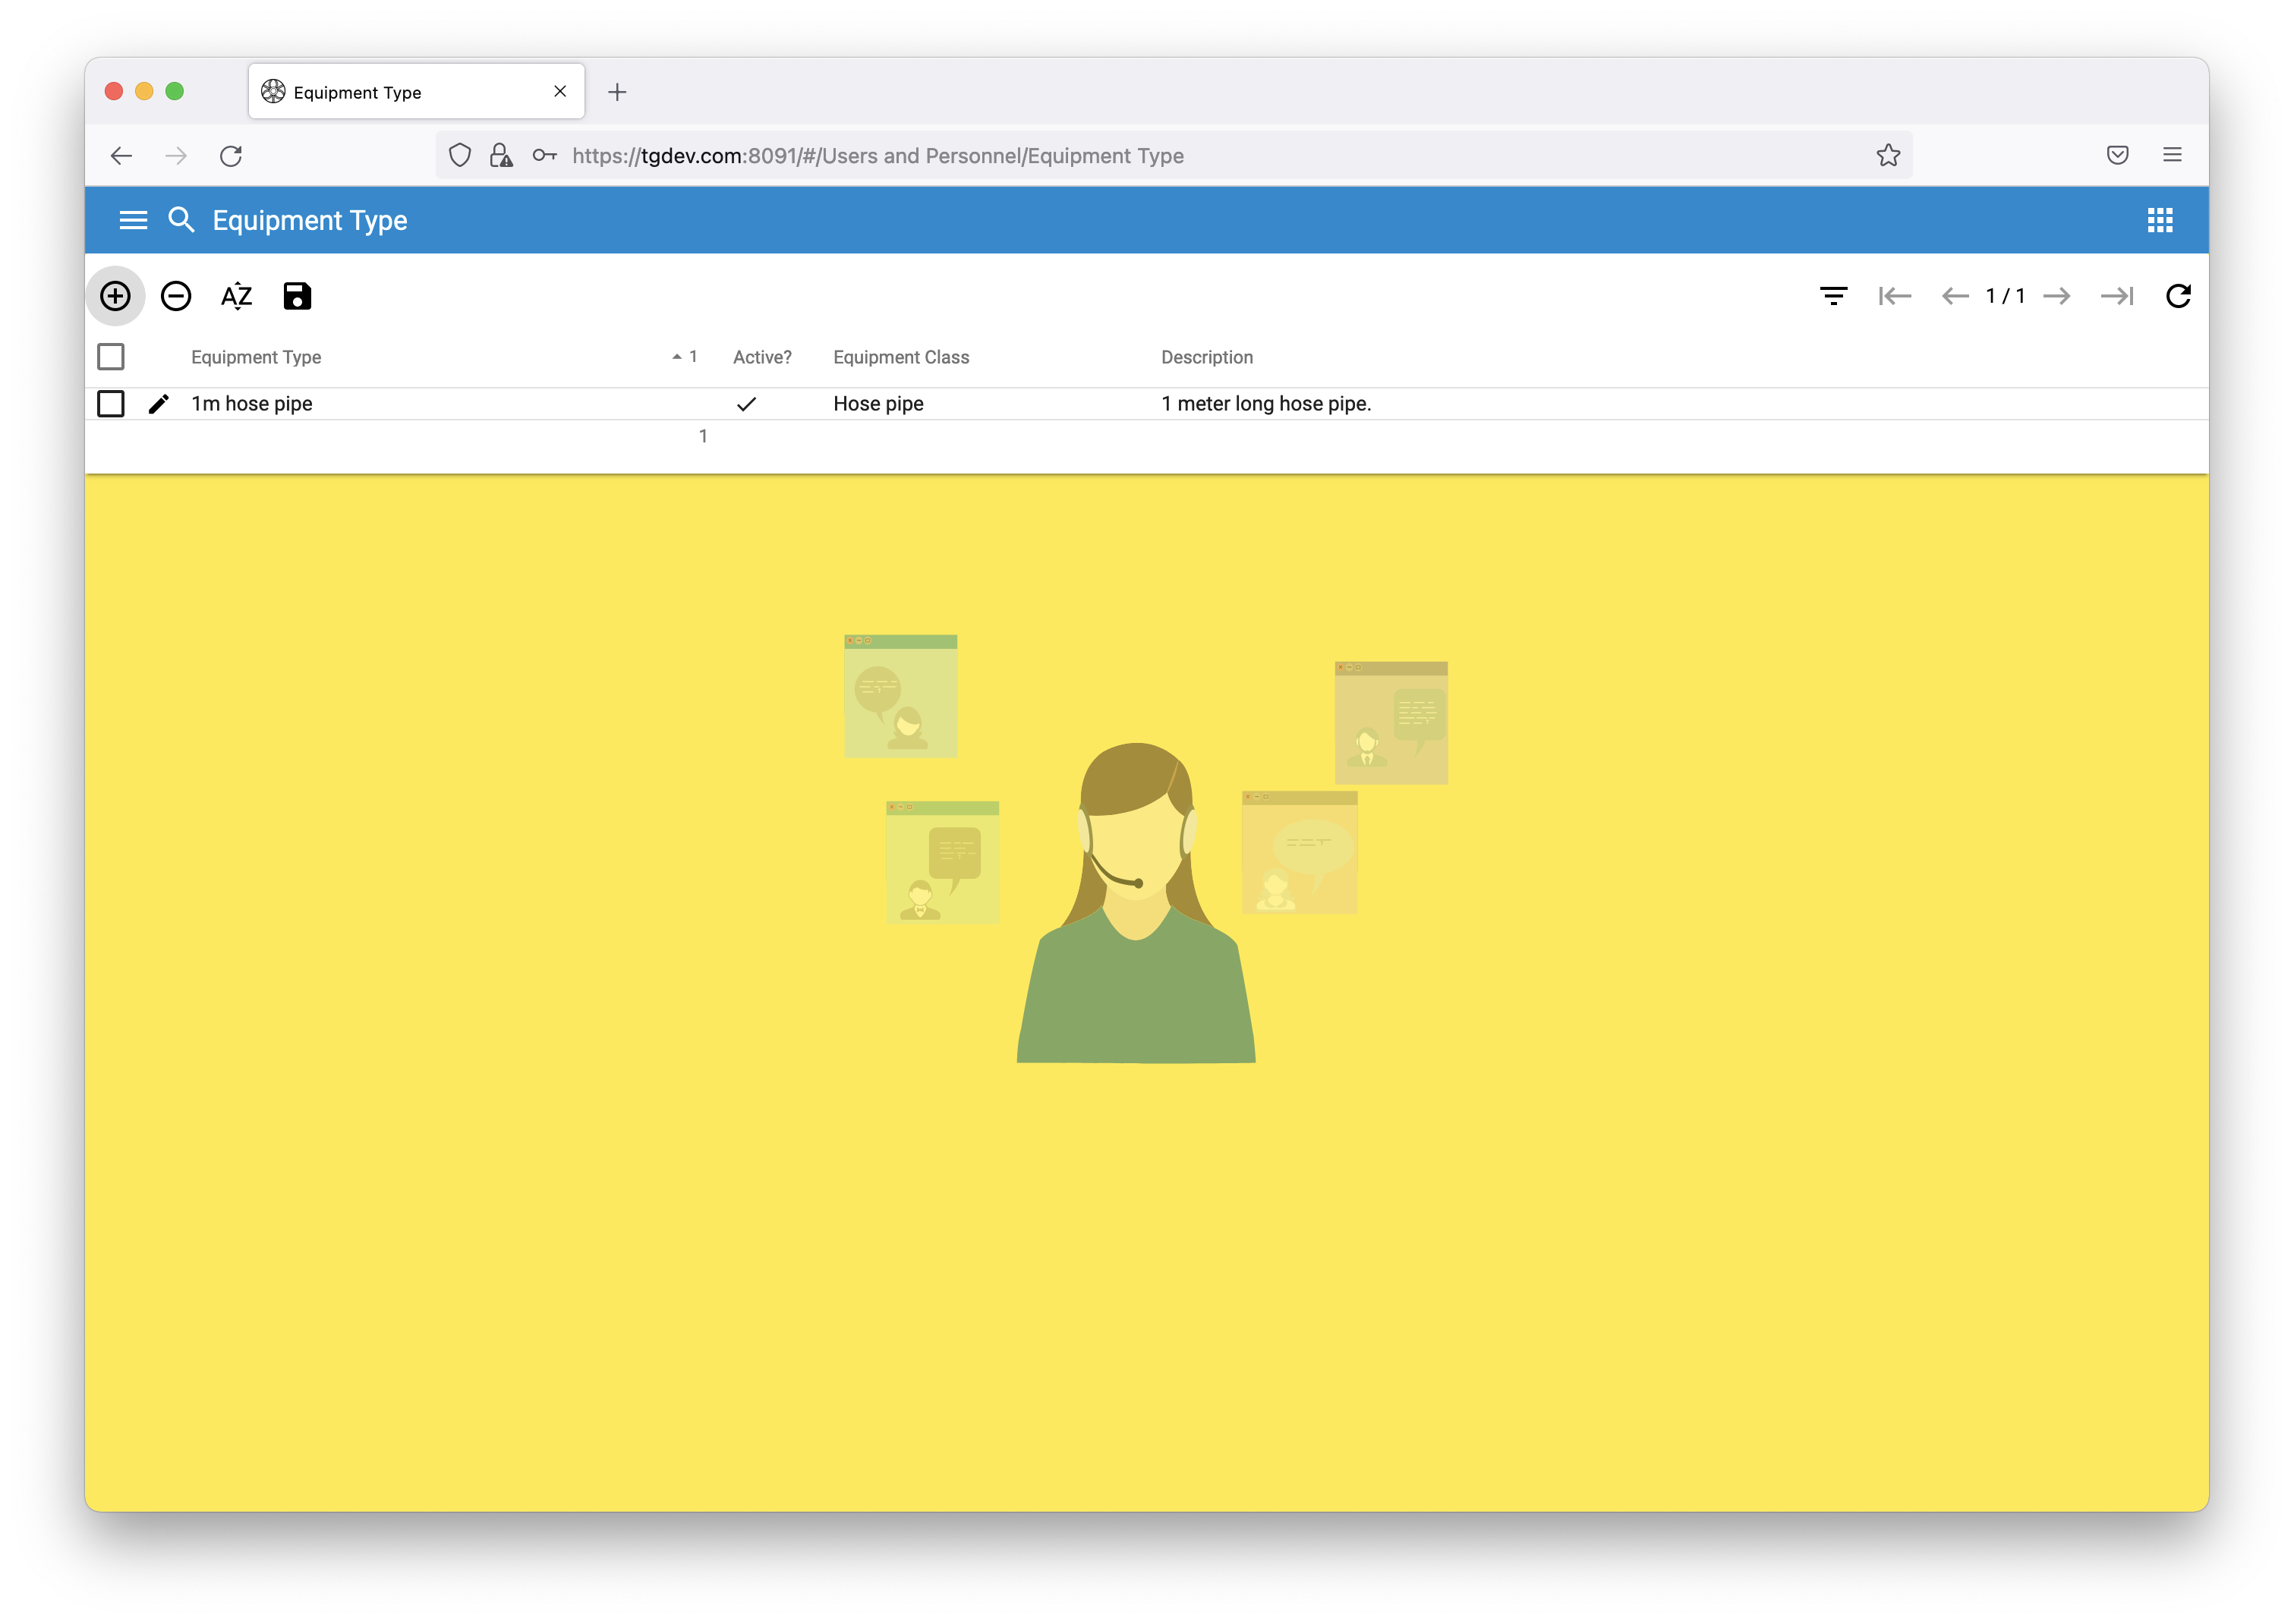
\includegraphics[width=0.95\linewidth]{sections/equipment/images/Fig.10.png}
	\caption{Equipment type search results.}\label{sections/equipment/images/Fig.10}
	\end{figure}

\newpage
Users can edit existing equipment types. As displayed on \hyperref[sections/equipment/images/Fig.11]{Fig.~\ref*{sections/equipment/images/Fig.11}}, users can edit title, activity status, equipment class and description of the specific equipment type.

    \begin{figure}[!htbp]
	\centering
	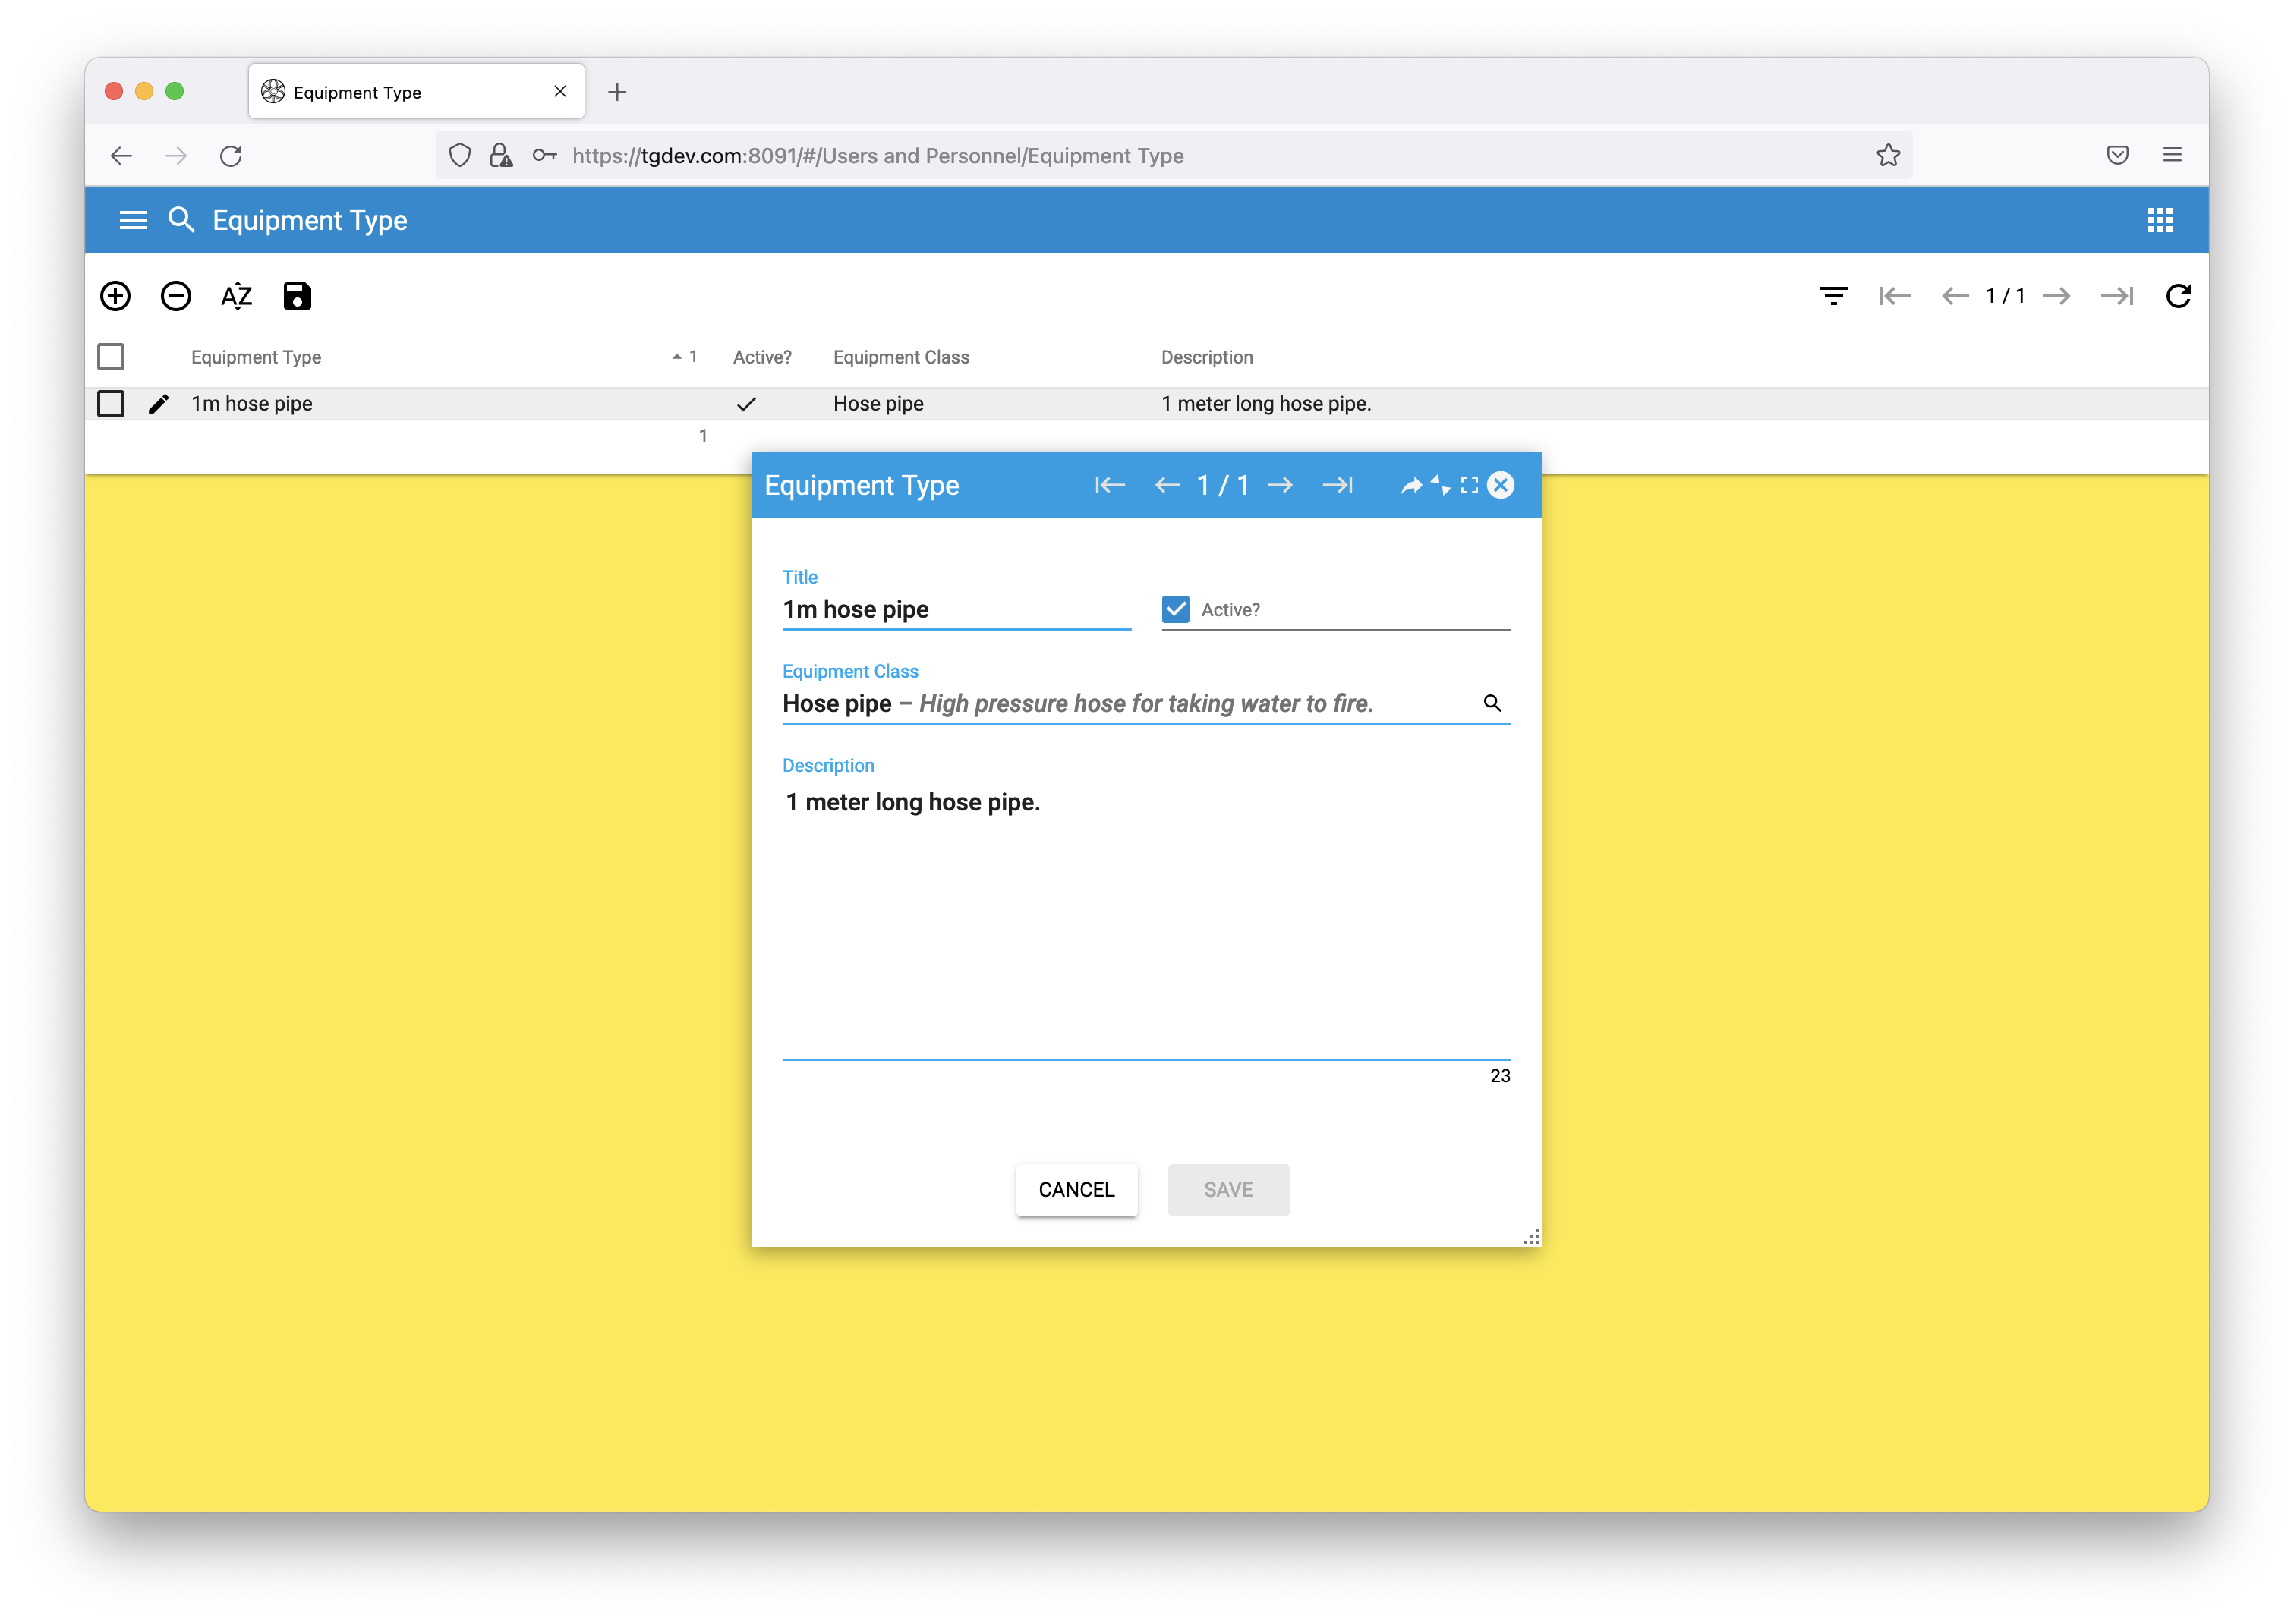
\includegraphics[width=0.95\linewidth]{sections/equipment/images/Fig.11.png}
	\caption{Equipment type editing.}\label{sections/equipment/images/Fig.11}
	\end{figure}
	
\newpage	
\subsection{Equipment}

In order to perform registration, classification and tracking of equipment correctly, users can create equipment. Possible equipment are pipe, lightning, etc. When creating a new equipment, users have to fill in its title without white spaces, activity status, equipment type and vehicle it belongs to, which are auto-completed, and its description, as displayed on \hyperref[sections/equipment/images/Fig.12]{Fig.~\ref*{sections/equipment/images/Fig.12}}. The number of equipment is auto-generated in chronological order after it was saved. 

    \begin{figure}[!htbp]
	\centering
	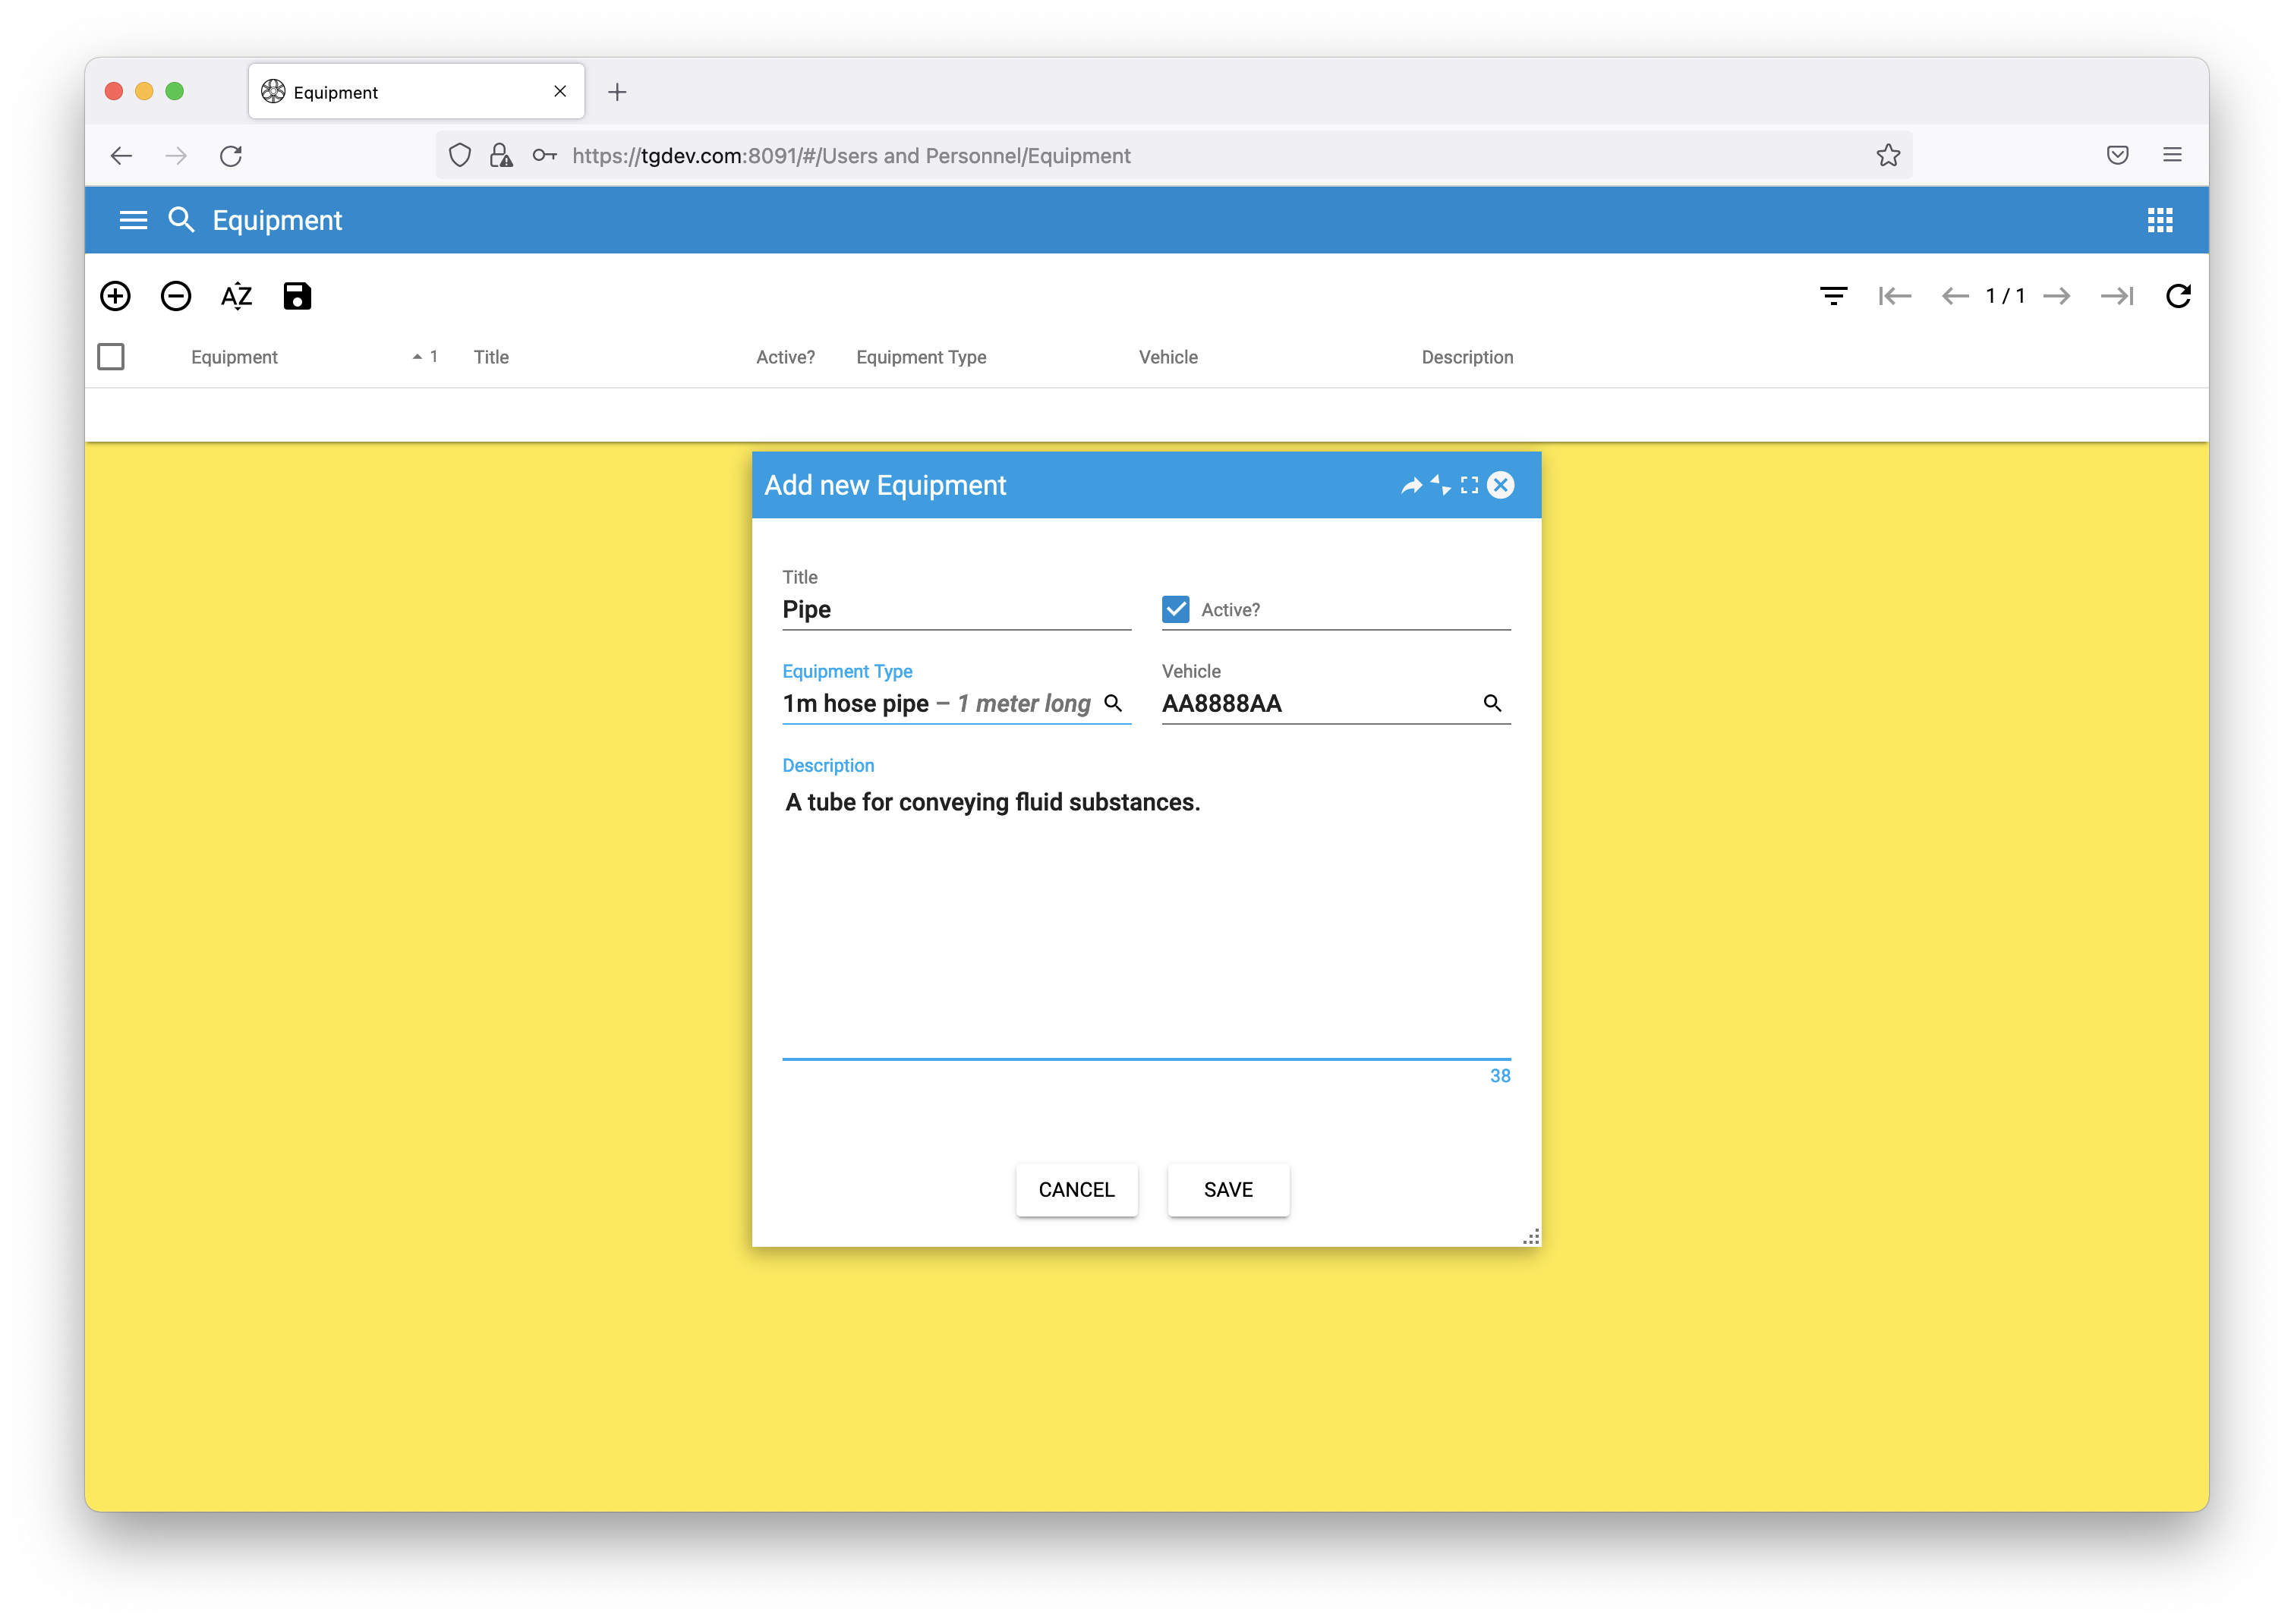
\includegraphics[width=0.95\linewidth]{sections/equipment/images/Fig.12.png}
	\caption{Equipment creation.}\label{sections/equipment/images/Fig.12}
	\end{figure}

\newpage
Users can search for existing equipment either by specifying number, which is auto-completed, activity status, title, equipment type and vehicle they belong to and which are auto-completed, or all, as displayed on \hyperref[sections/equipment/images/Fig.13]{Fig.~\ref*{sections/equipment/images/Fig.13}}.

    \begin{figure}[!htbp]
	\centering
	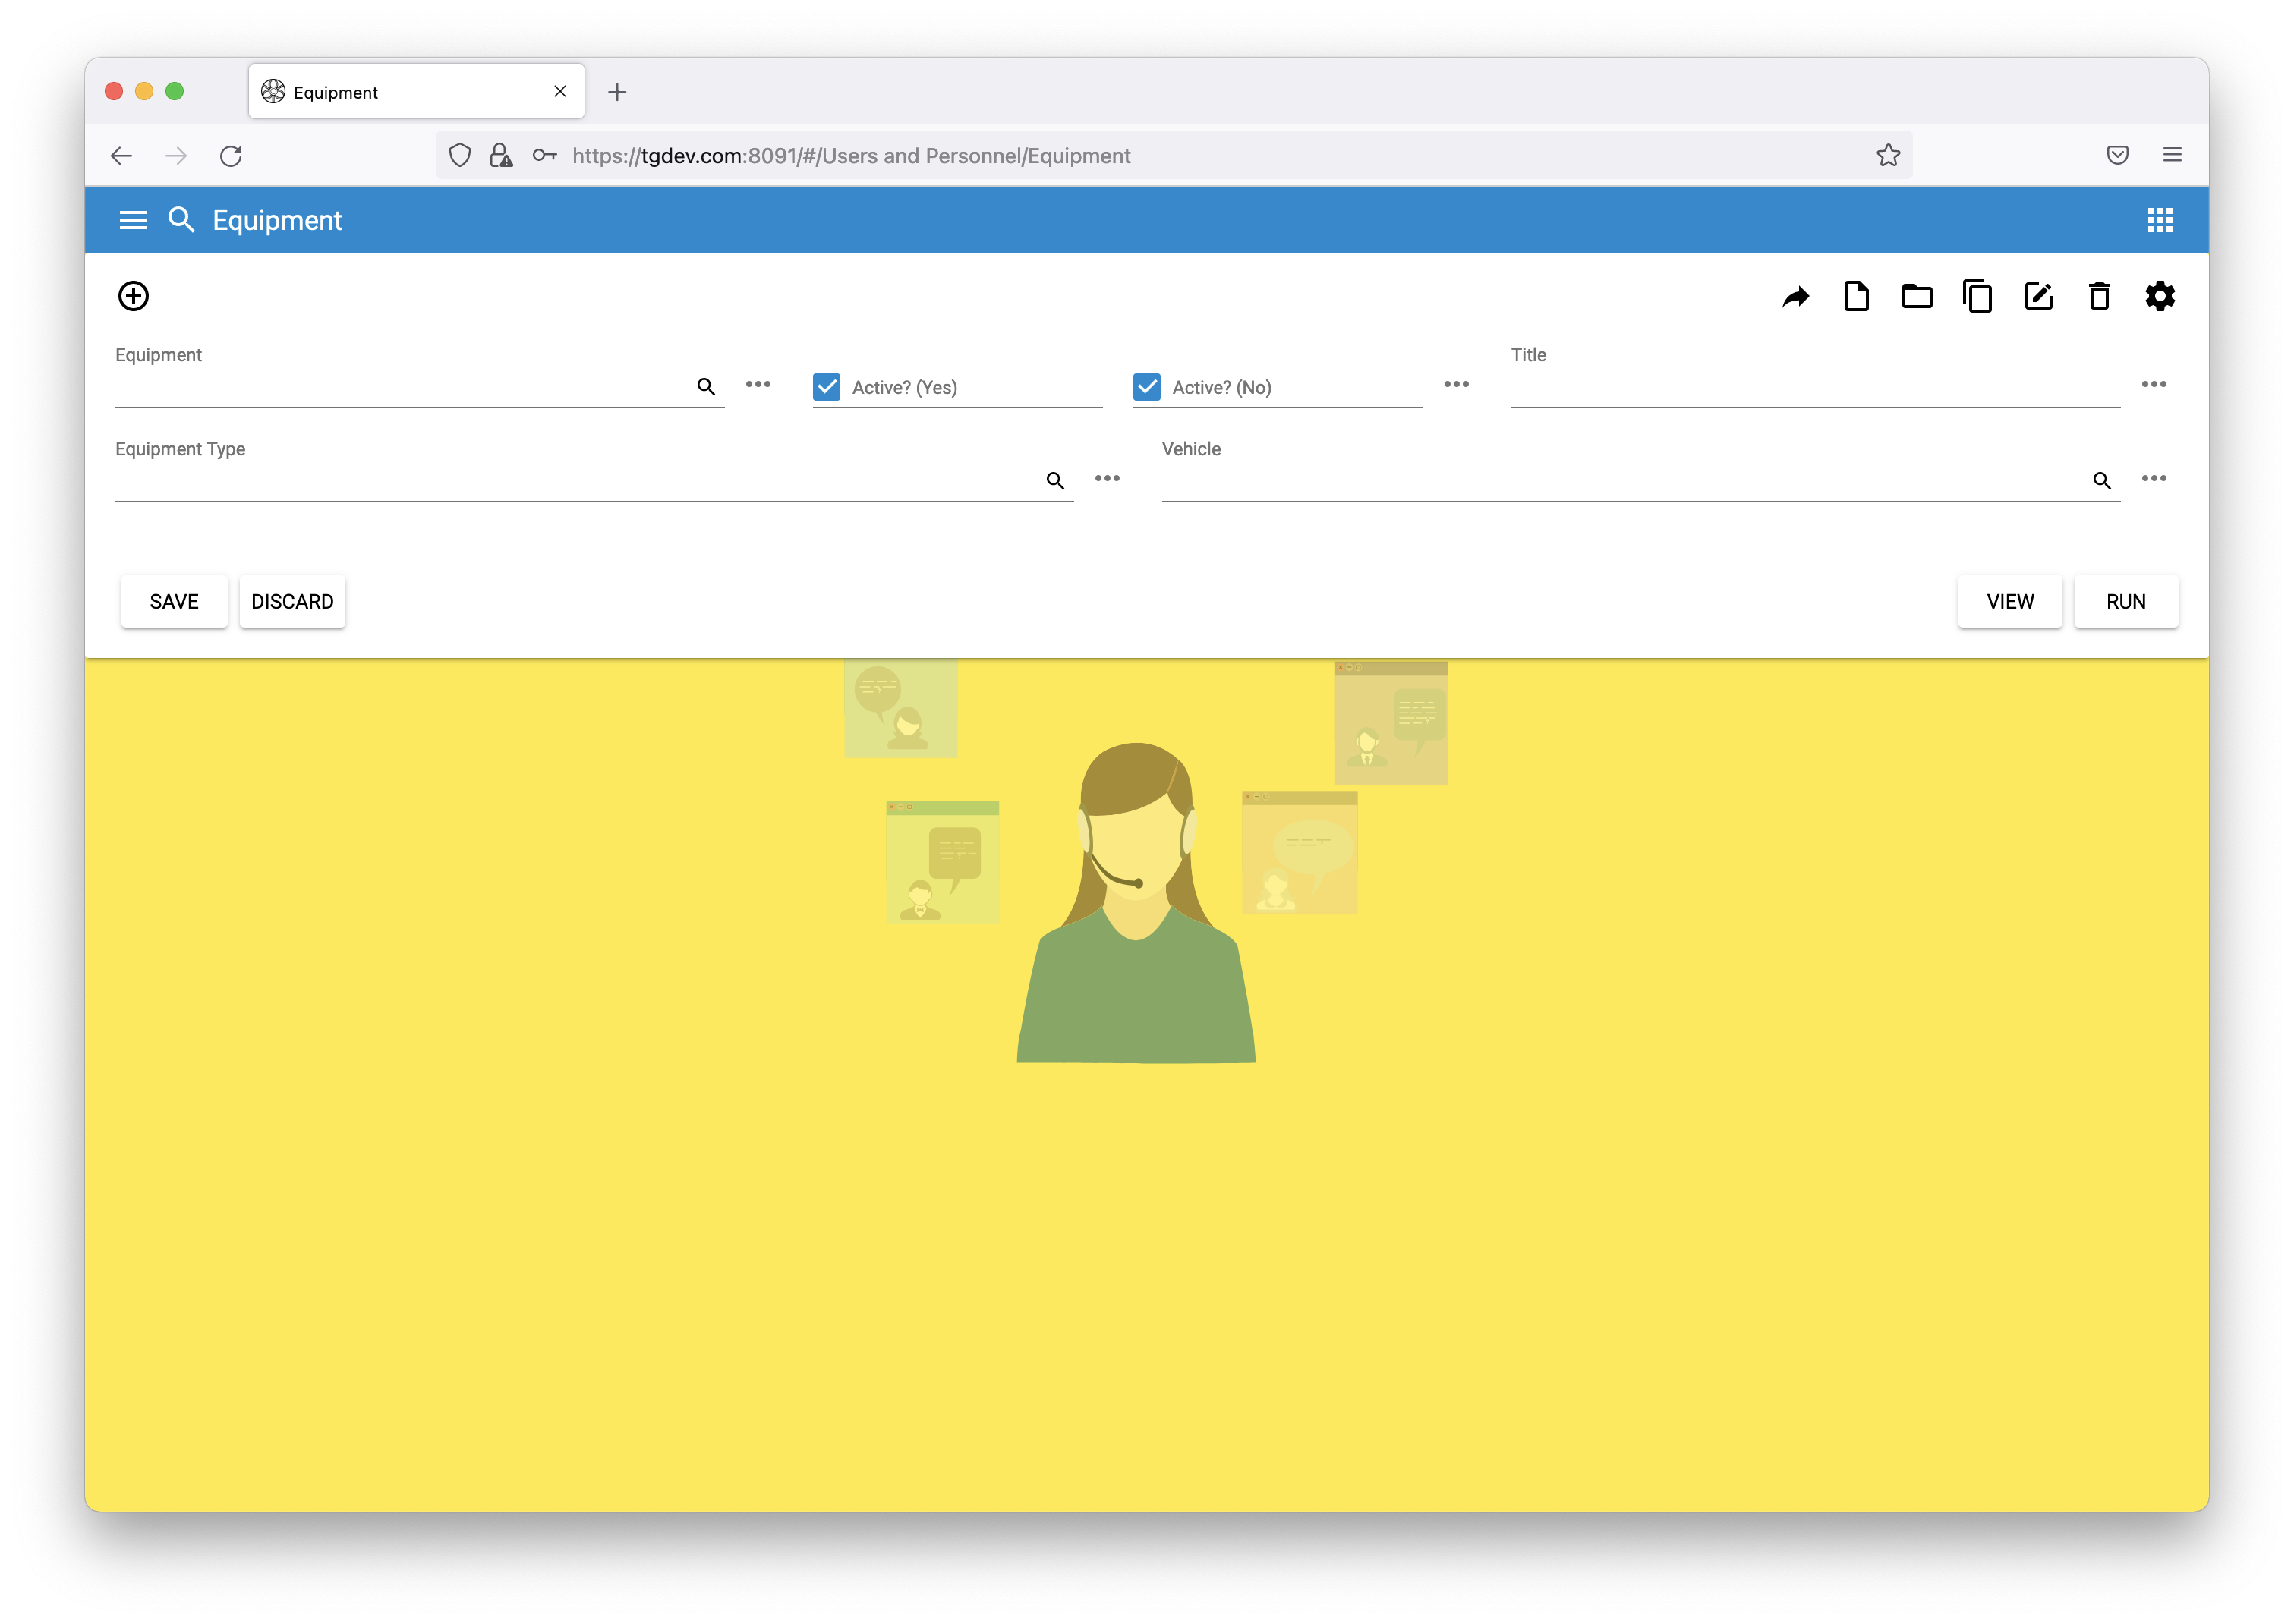
\includegraphics[width=0.95\linewidth]{sections/equipment/images/Fig.13.png}
	\caption{Equipment search query.}\label{sections/equipment/images/Fig.13}
	\end{figure}
	
\newpage
Search results are displayed along with number, title, activity status, equipment type, vehicle and description of the relevant equipment, as displayed on \hyperref[sections/equipment/images/Fig.14]{Fig.~\ref*{sections/equipment/images/Fig.14}}.

    \begin{figure}[!htbp]
	\centering
	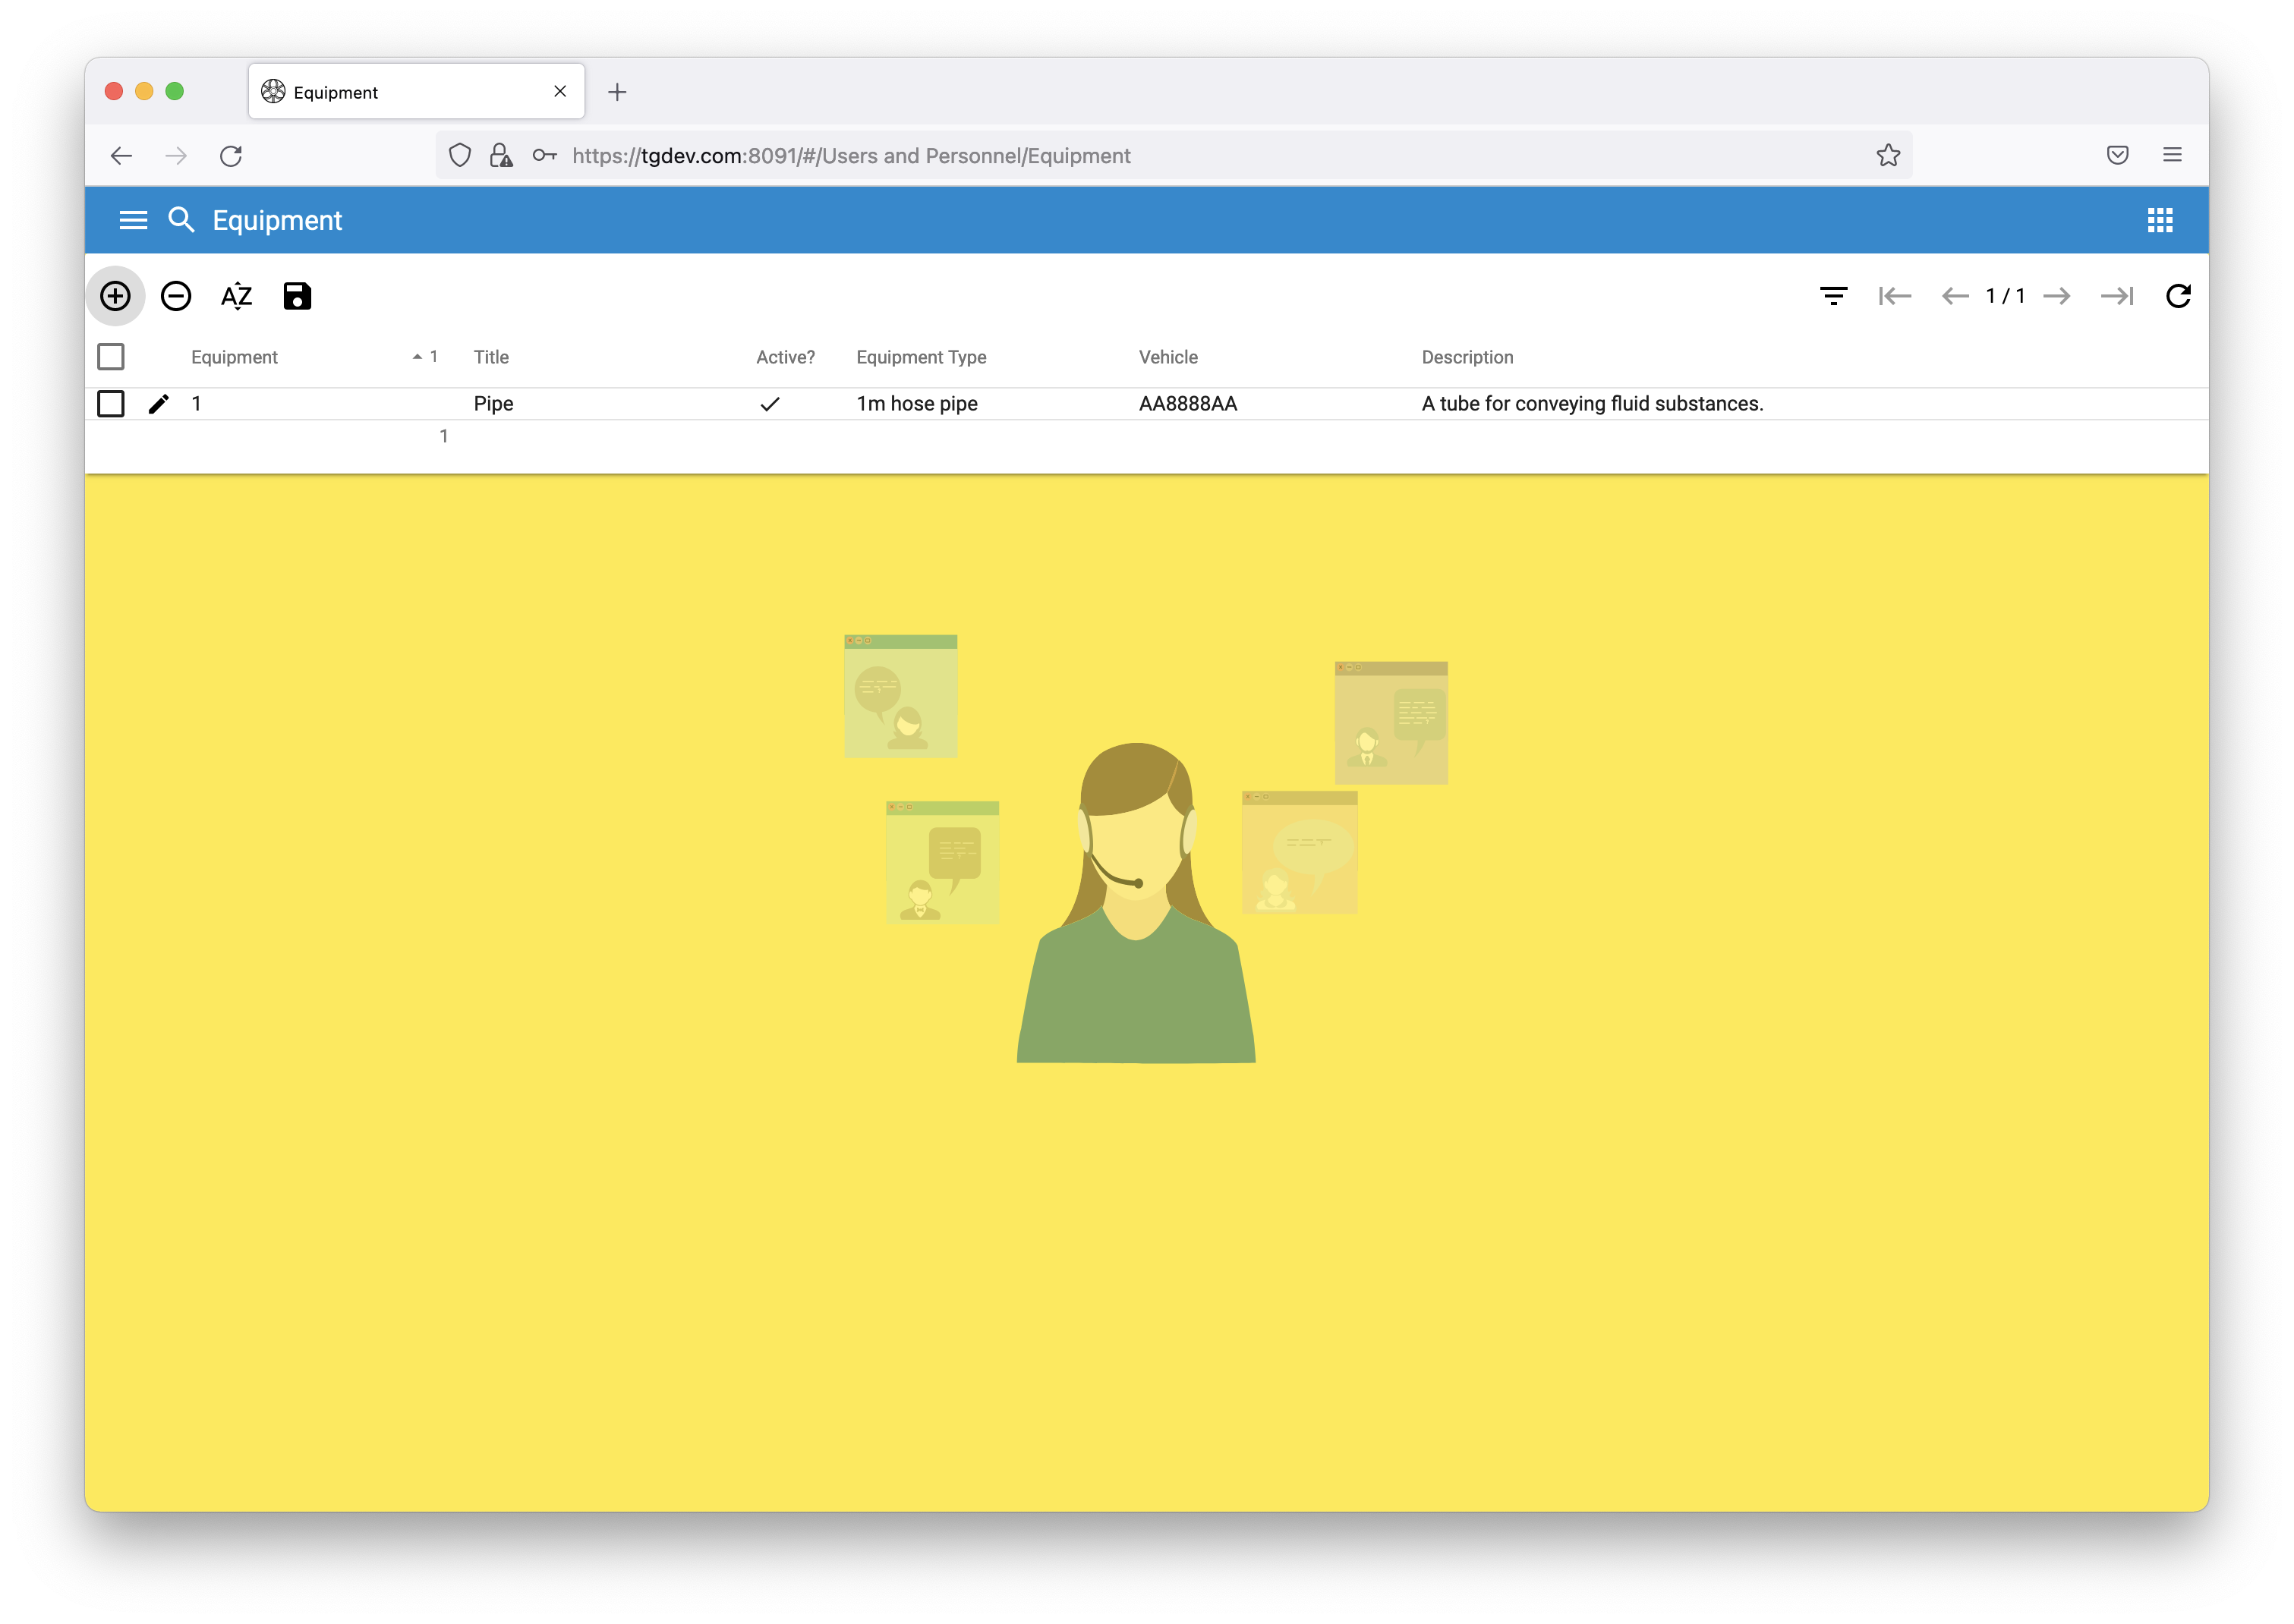
\includegraphics[width=0.95\linewidth]{sections/equipment/images/Fig.14.png}
	\caption{Equipment search results.}\label{sections/equipment/images/Fig.14}
	\end{figure}

\newpage
Users can edit existing equipment. As displayed on \hyperref[sections/equipment/images/Fig.15]{Fig.~\ref*{sections/equipment/images/Fig.15}}, users can edit title, activity status, equipment type, vehicle and description of the specific equipment.

    \begin{figure}[!htbp]
	\centering
	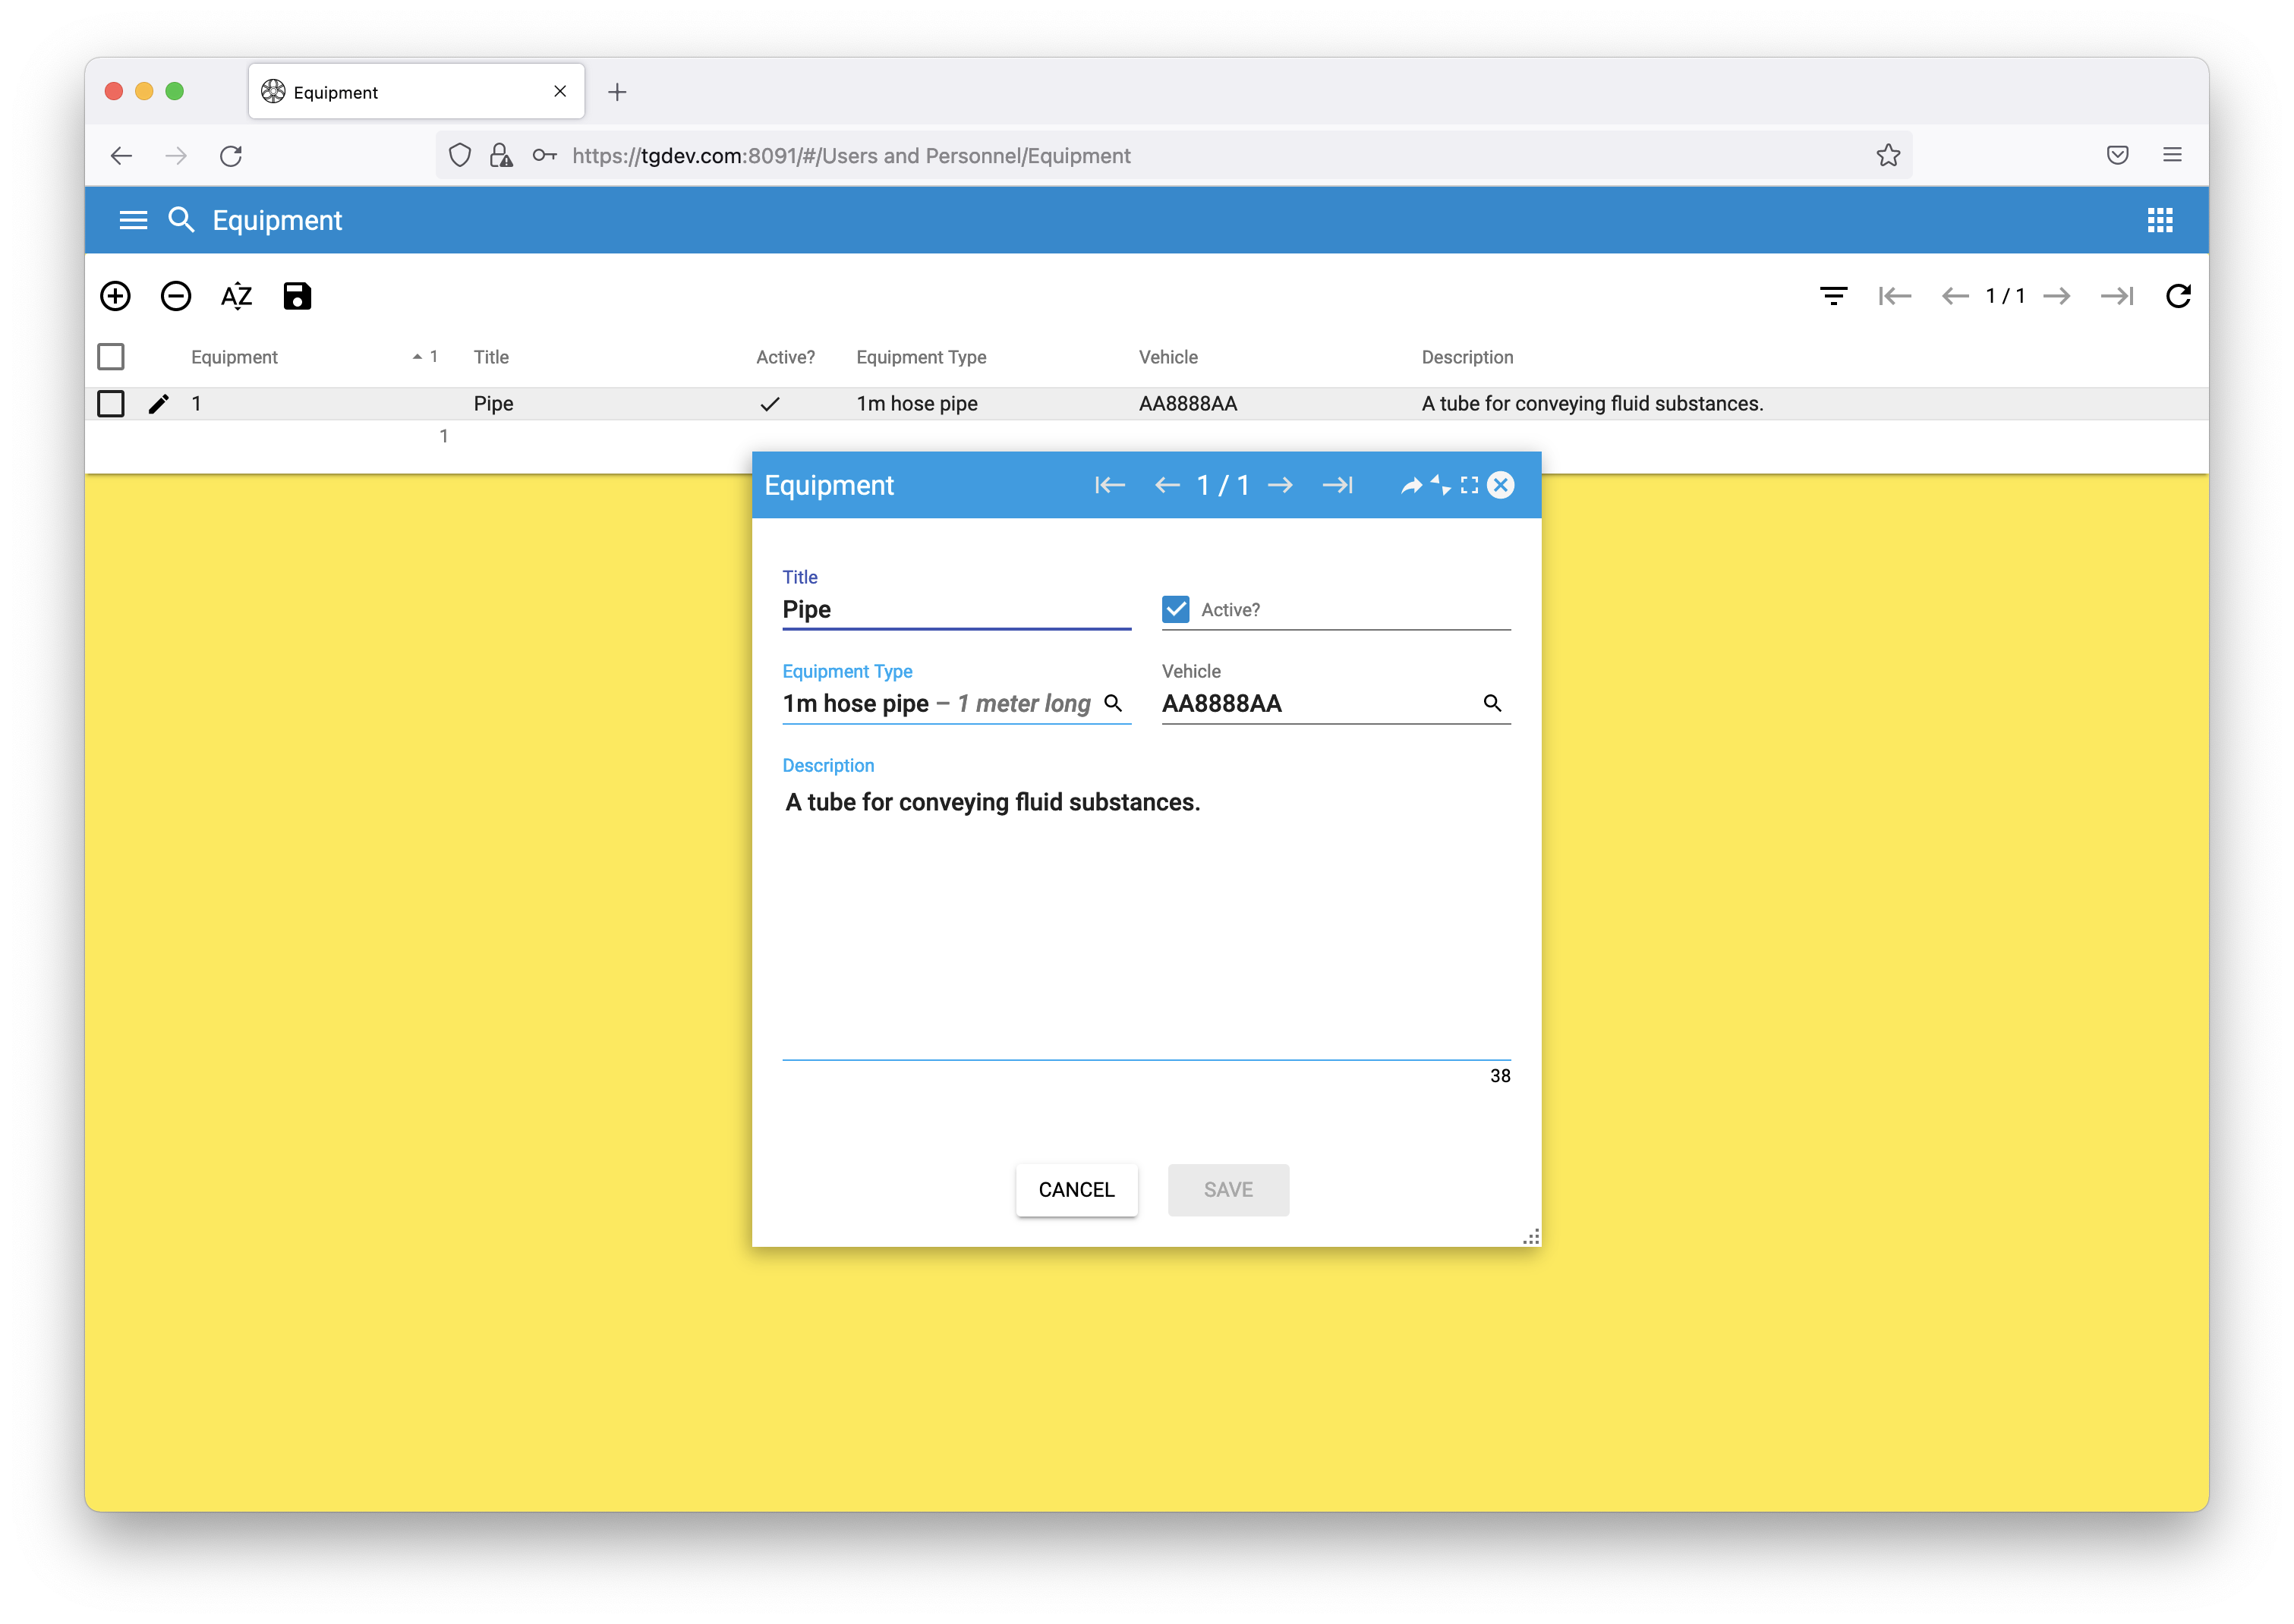
\includegraphics[width=0.95\linewidth]{sections/equipment/images/Fig.15.png}
	\caption{Equipment editing.}\label{sections/equipment/images/Fig.15}
	\end{figure}
    \section{Vehicles Module}\label{sec:01}

\subsection{Vehicle Type}

In order to perform classification of vehicles correctly, users can create vehicle types. Possible vehicle types are hose aerial truck, fire truck, heavy rescue truck, water tender, etc. When creating a new vehicle type, users have to fill in its title without white spaces and activity status, as well as its description, as displayed on \hyperref[sections/vehicles/images/20]{Fig.~\ref*{sections/vehicles/images/20}}. 

    \begin{figure}[!htbp]
	\centering
	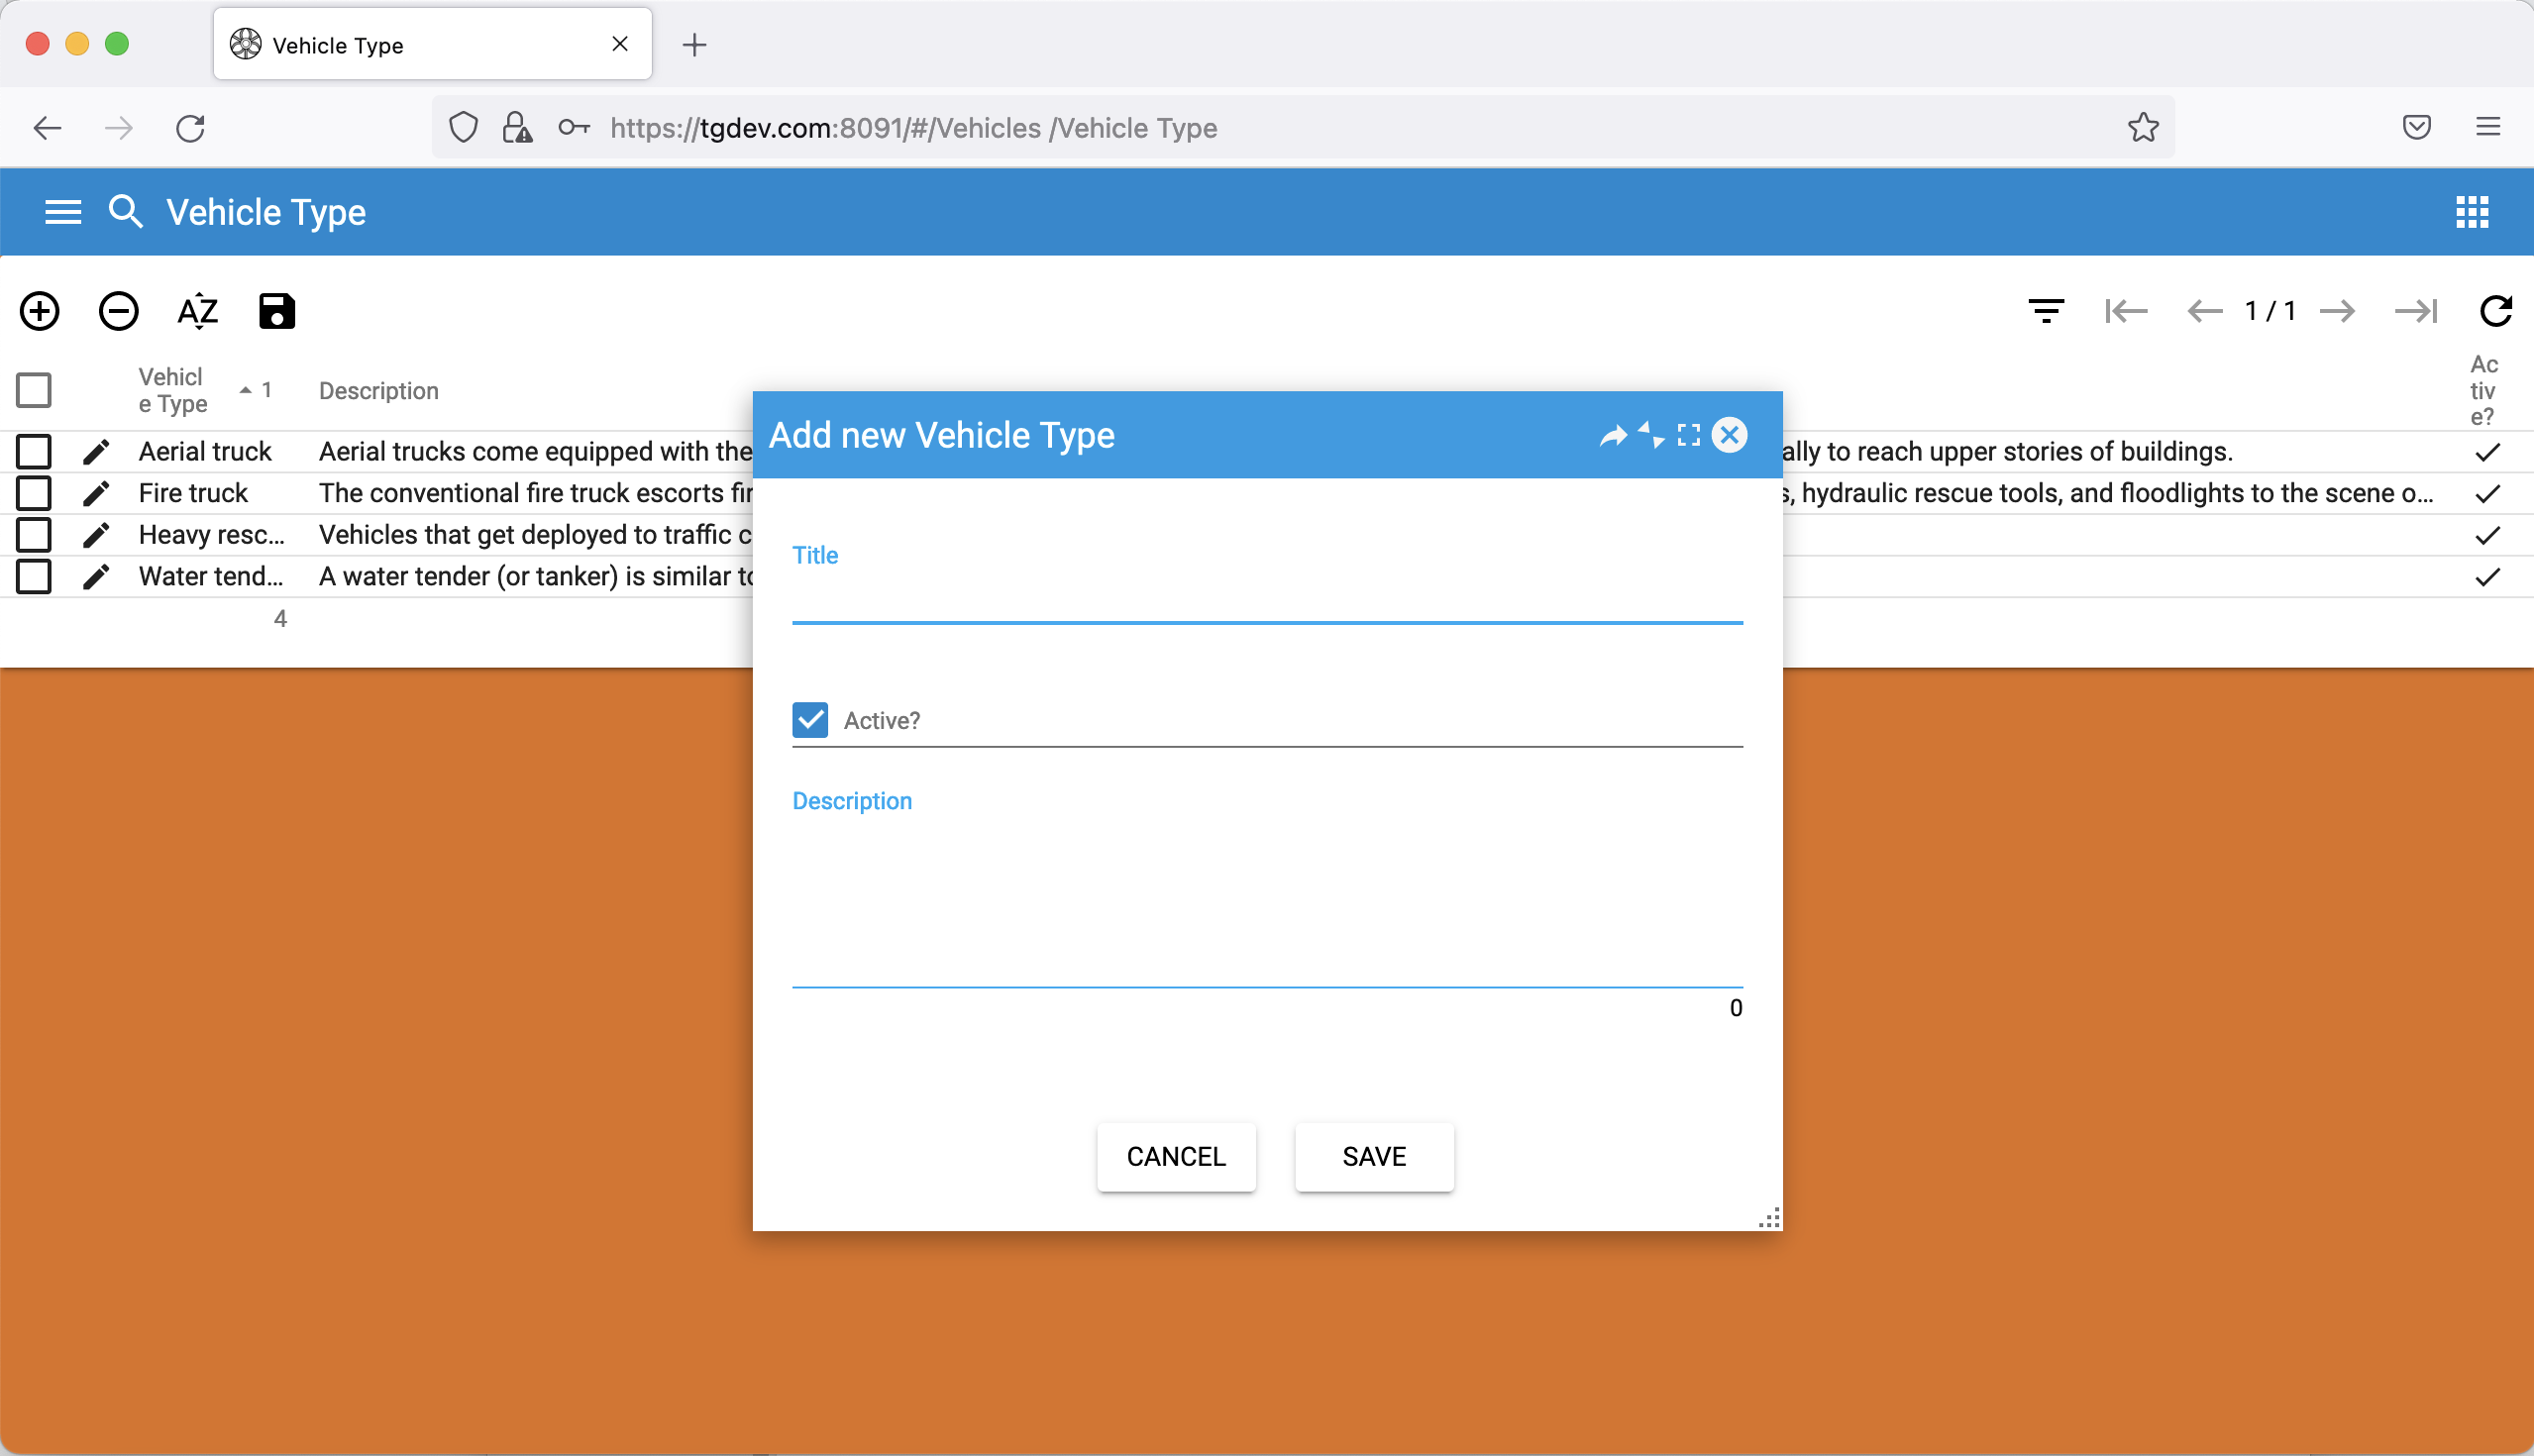
\includegraphics[width=0.95\linewidth]{sections/vehicles/images/20.png}
	\caption{Vehicle type creation.}\label{sections/vehicles/images/20}
	\end{figure}

\newpage
Users can search for existing vehicle types either by specifying title, which is auto-completed, or activity status, or description or all of them as displayed on
\hyperref[sections/vehicles/images/21]{Fig.~\ref*{sections/vehicles/images/21}}.

    \begin{figure}[!htbp]
	\centering
	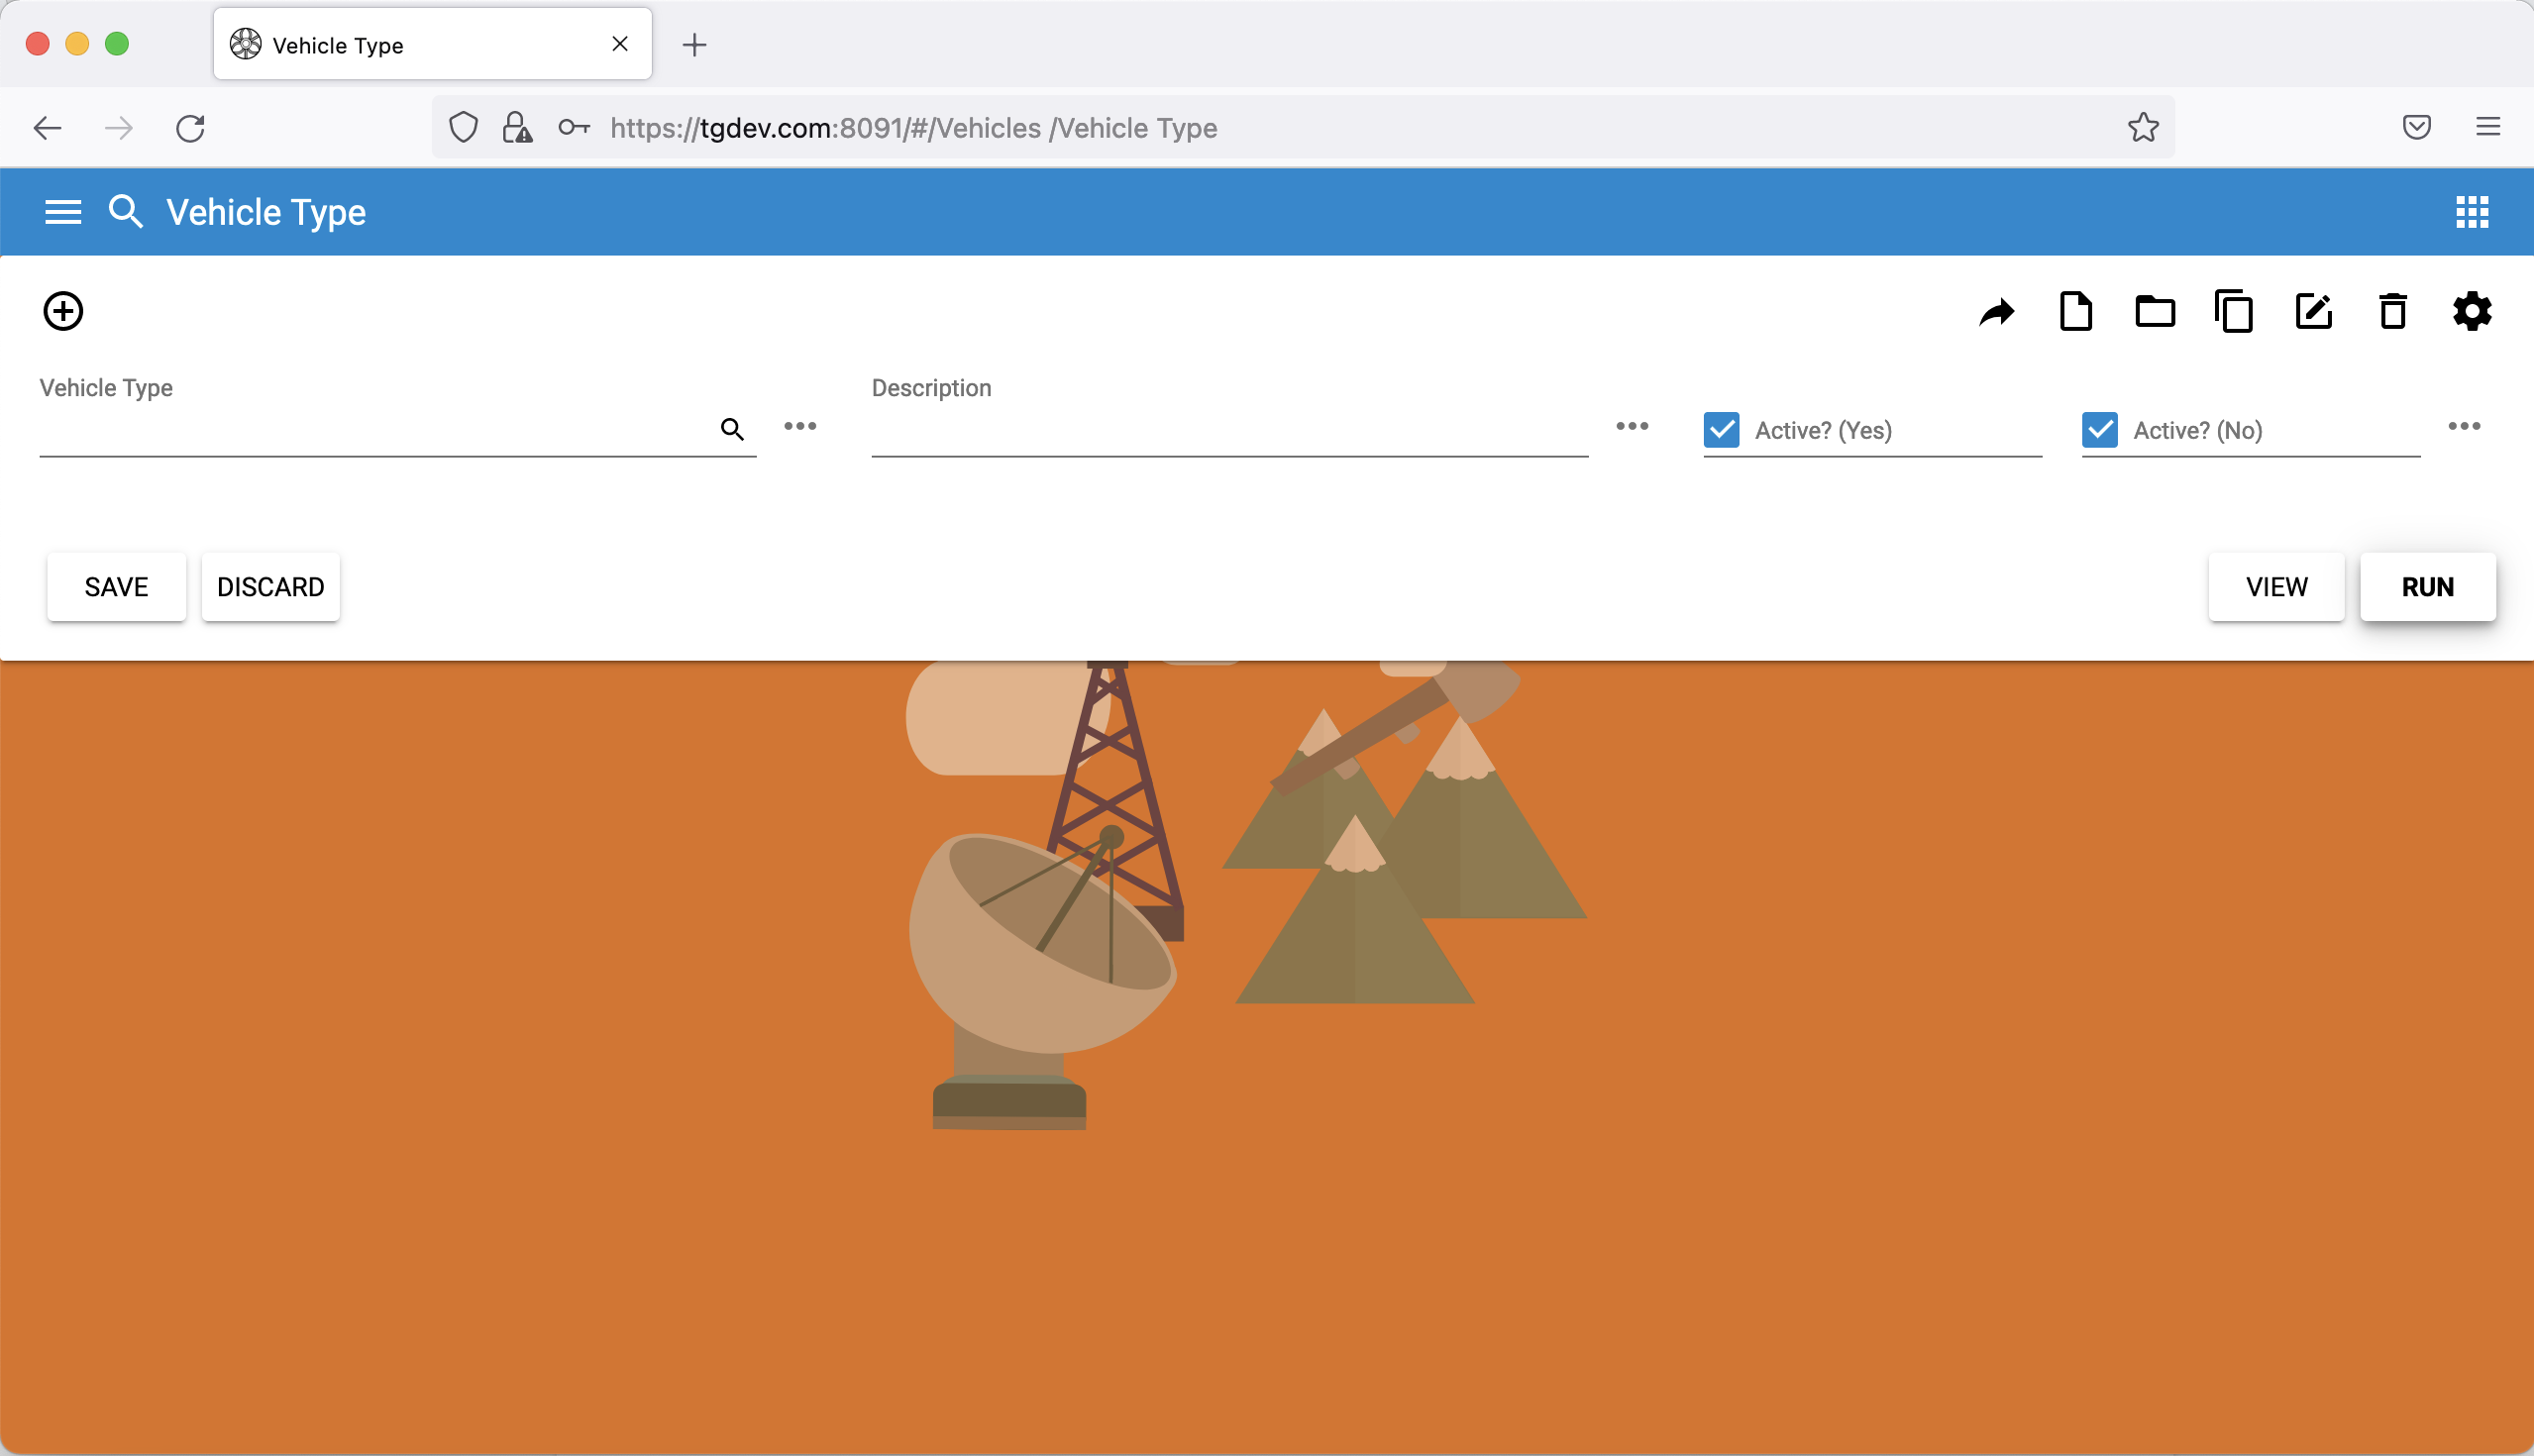
\includegraphics[width=0.95\linewidth]{sections/vehicles/images/21.png}
	\caption{Vehicle type search query.}\label{sections/vehicles/images/21}
	\end{figure}
	
\newpage
Search results are displayed along with title, activity status and description of the relevant vehicle types, as displayed on \hyperref[sections/vehicles/images/22]{Fig.~\ref*{sections/vehicles/images/22}}.

    \begin{figure}[!htbp]
	\centering
	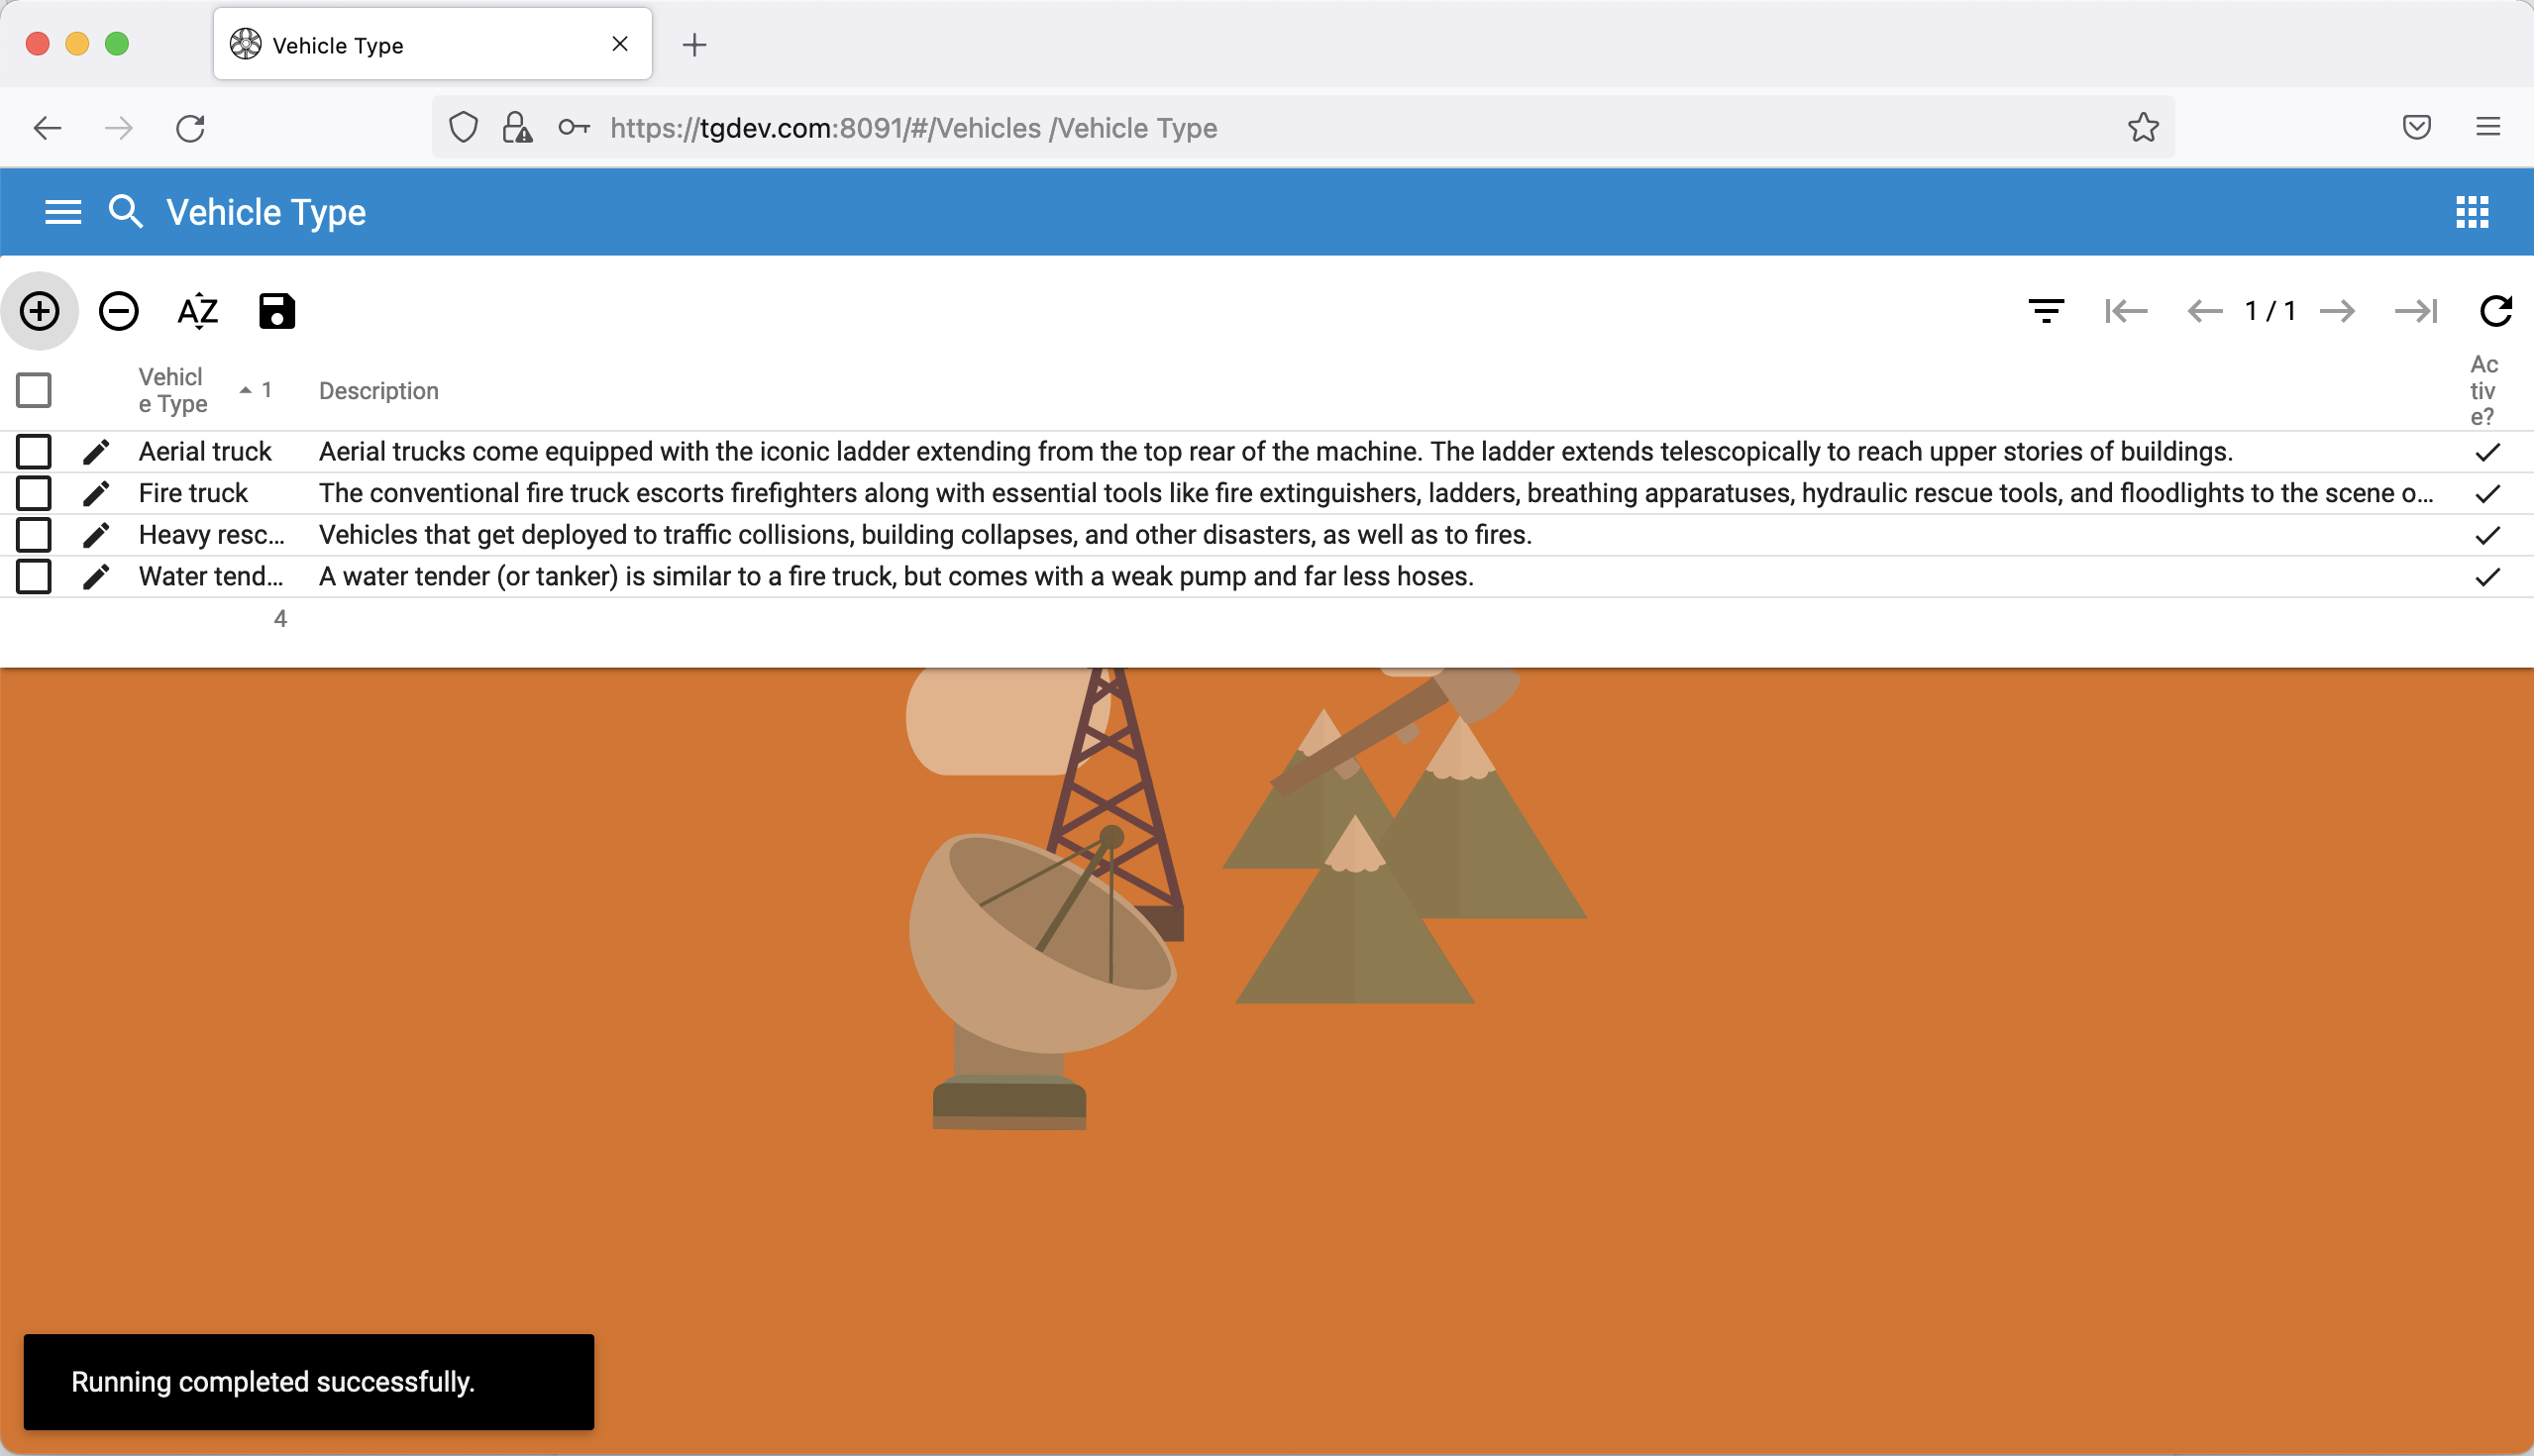
\includegraphics[width=0.95\linewidth]{sections/vehicles/images/22.png}
	\caption{Vehicle type search results.}\label{sections/vehicles/images/22}
	\end{figure}

\newpage
Users can edit existing vehicle types. On the main tab, as displayed on \hyperref[sections/vehicles/images/23]{Fig.~\ref*{sections/vehicles/images/23}}, users can edit title, activity status and description of the specific vehicle type.


    \begin{figure}[!htbp]
	\centering
	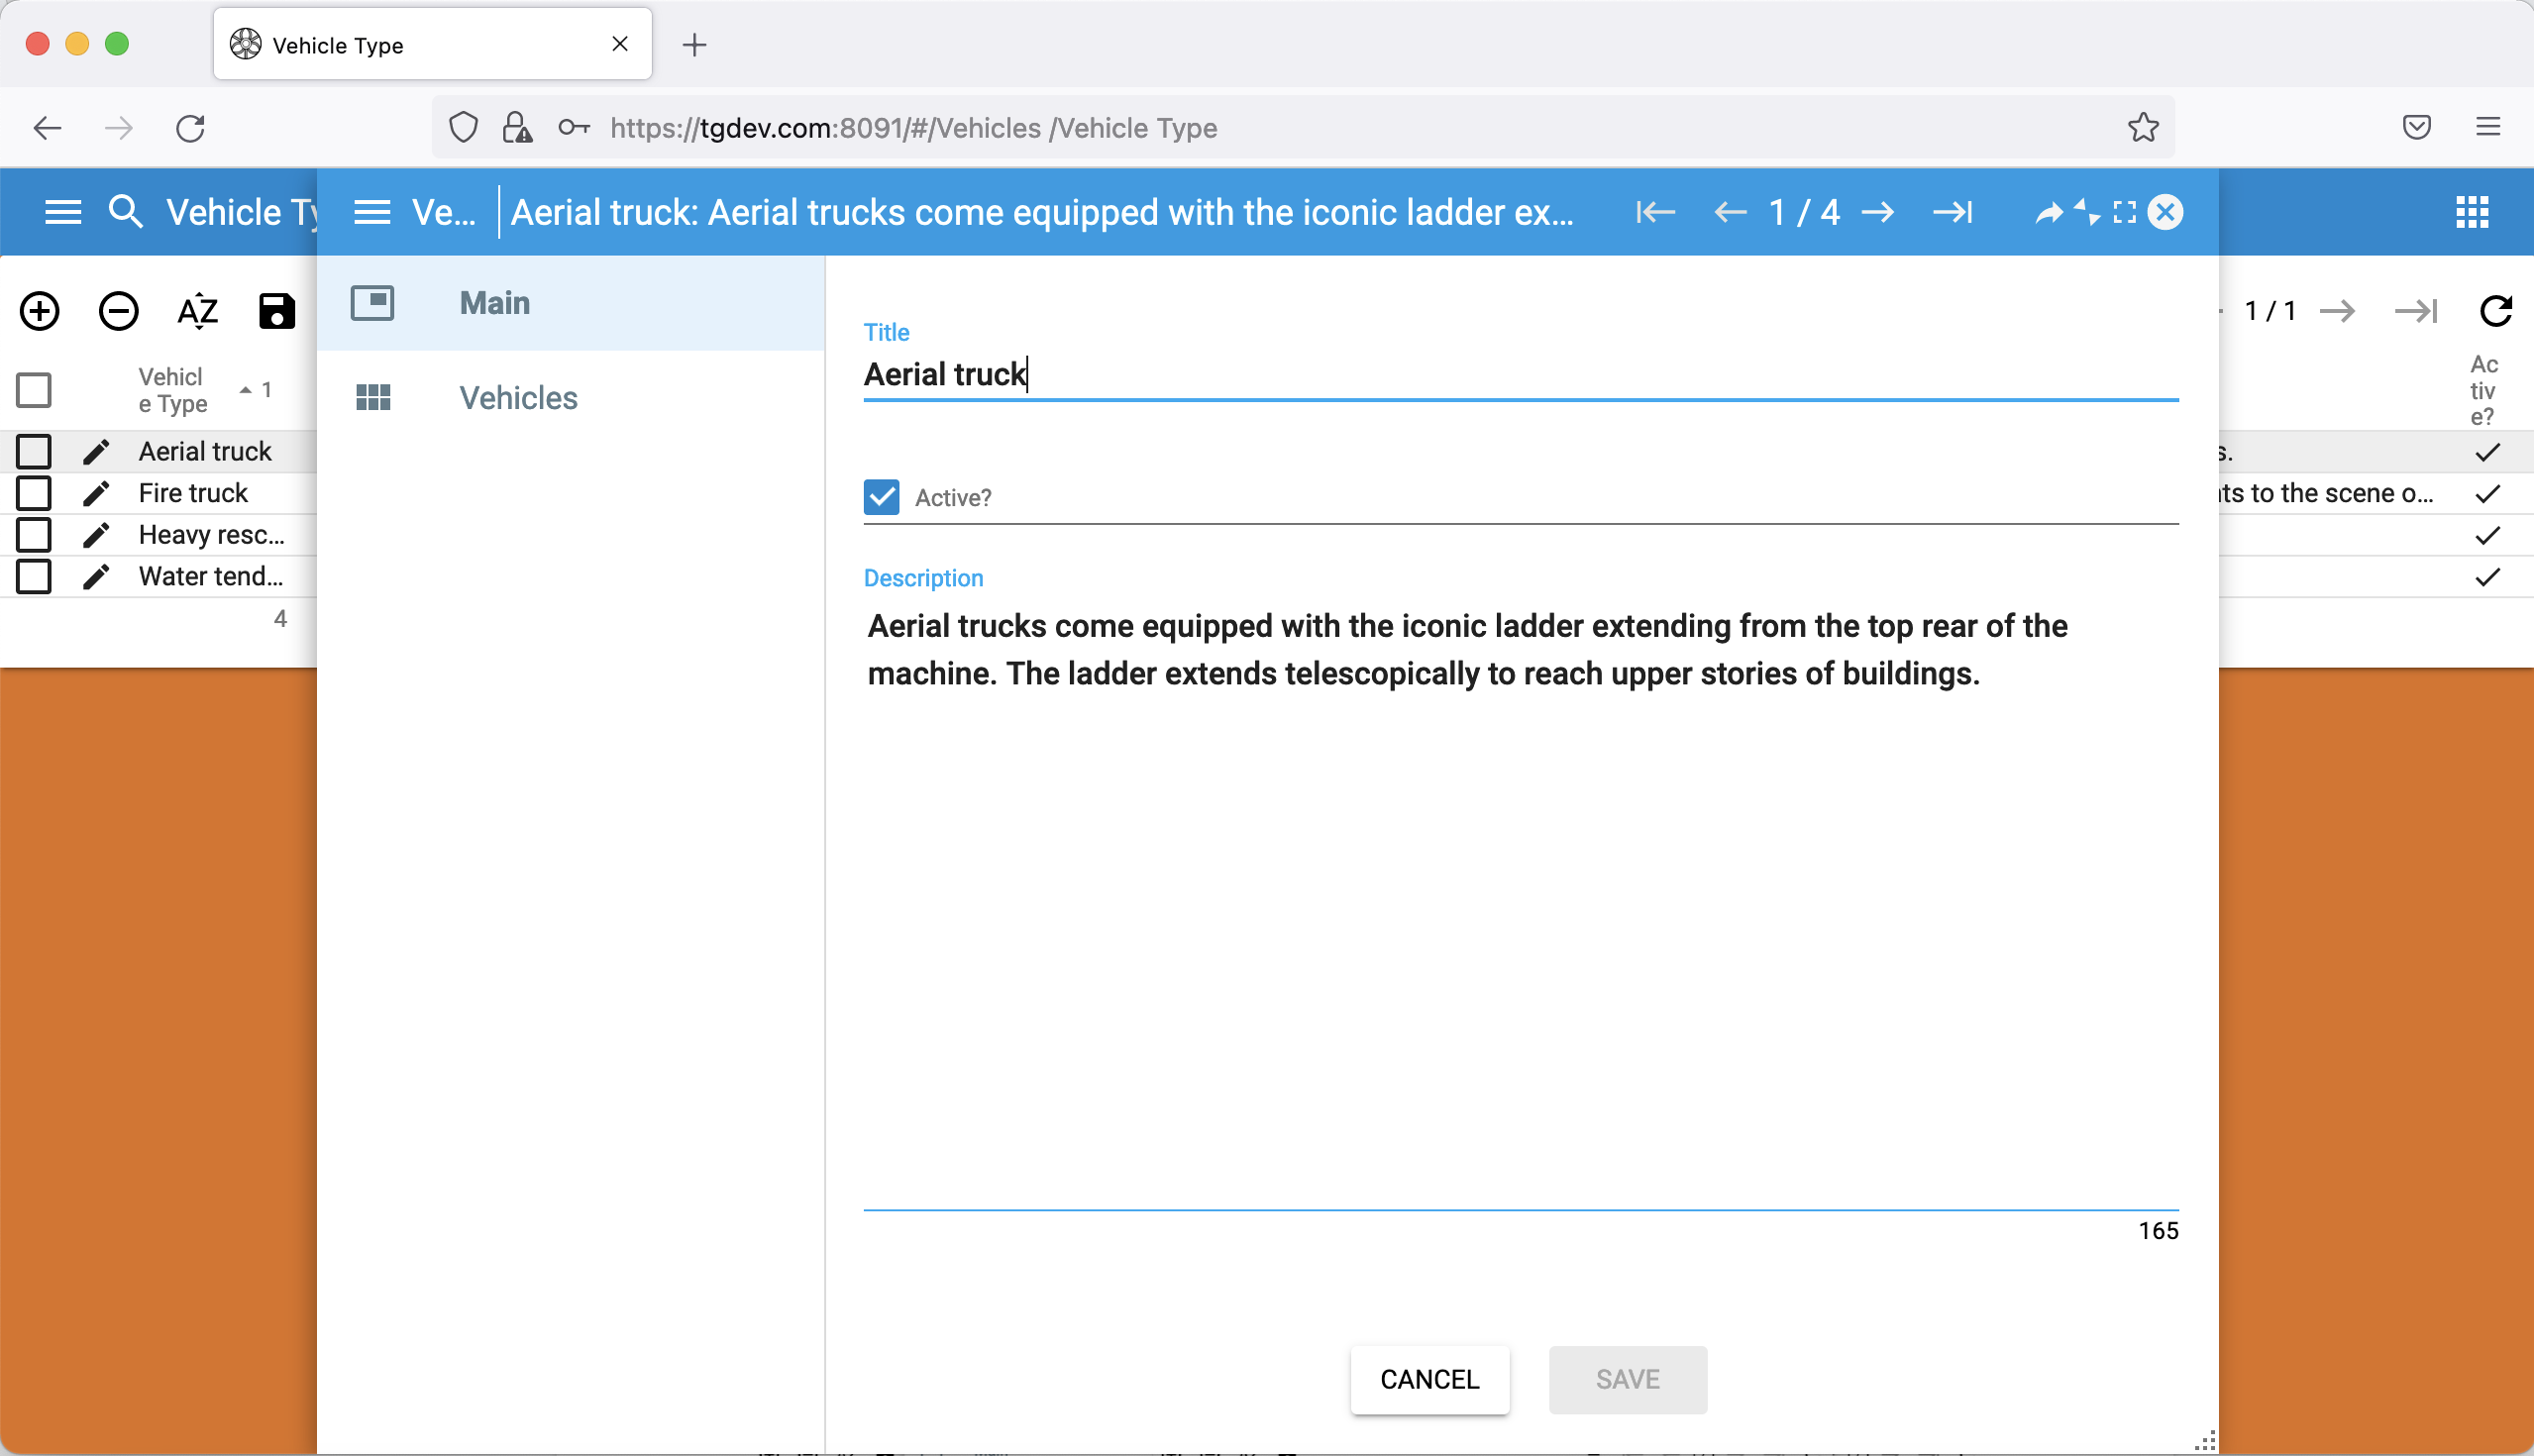
\includegraphics[width=0.95\linewidth]{sections/vehicles/images/23.png}
	\caption{Vehicle type editing.}\label{sections/vehicles/images/23}
	\end{figure}
	
\newpage	
On the ‘Vehicles’ tab, users can observe all of the vehicles related only to this specific vehicle type along with number, activity status, model, assigned driver, and description, as displayed on \hyperref[sections/vehicles/images/24]{Fig.~\ref*{sections/vehicles/images/24}}.

    \begin{figure}[!htbp]
	\centering
	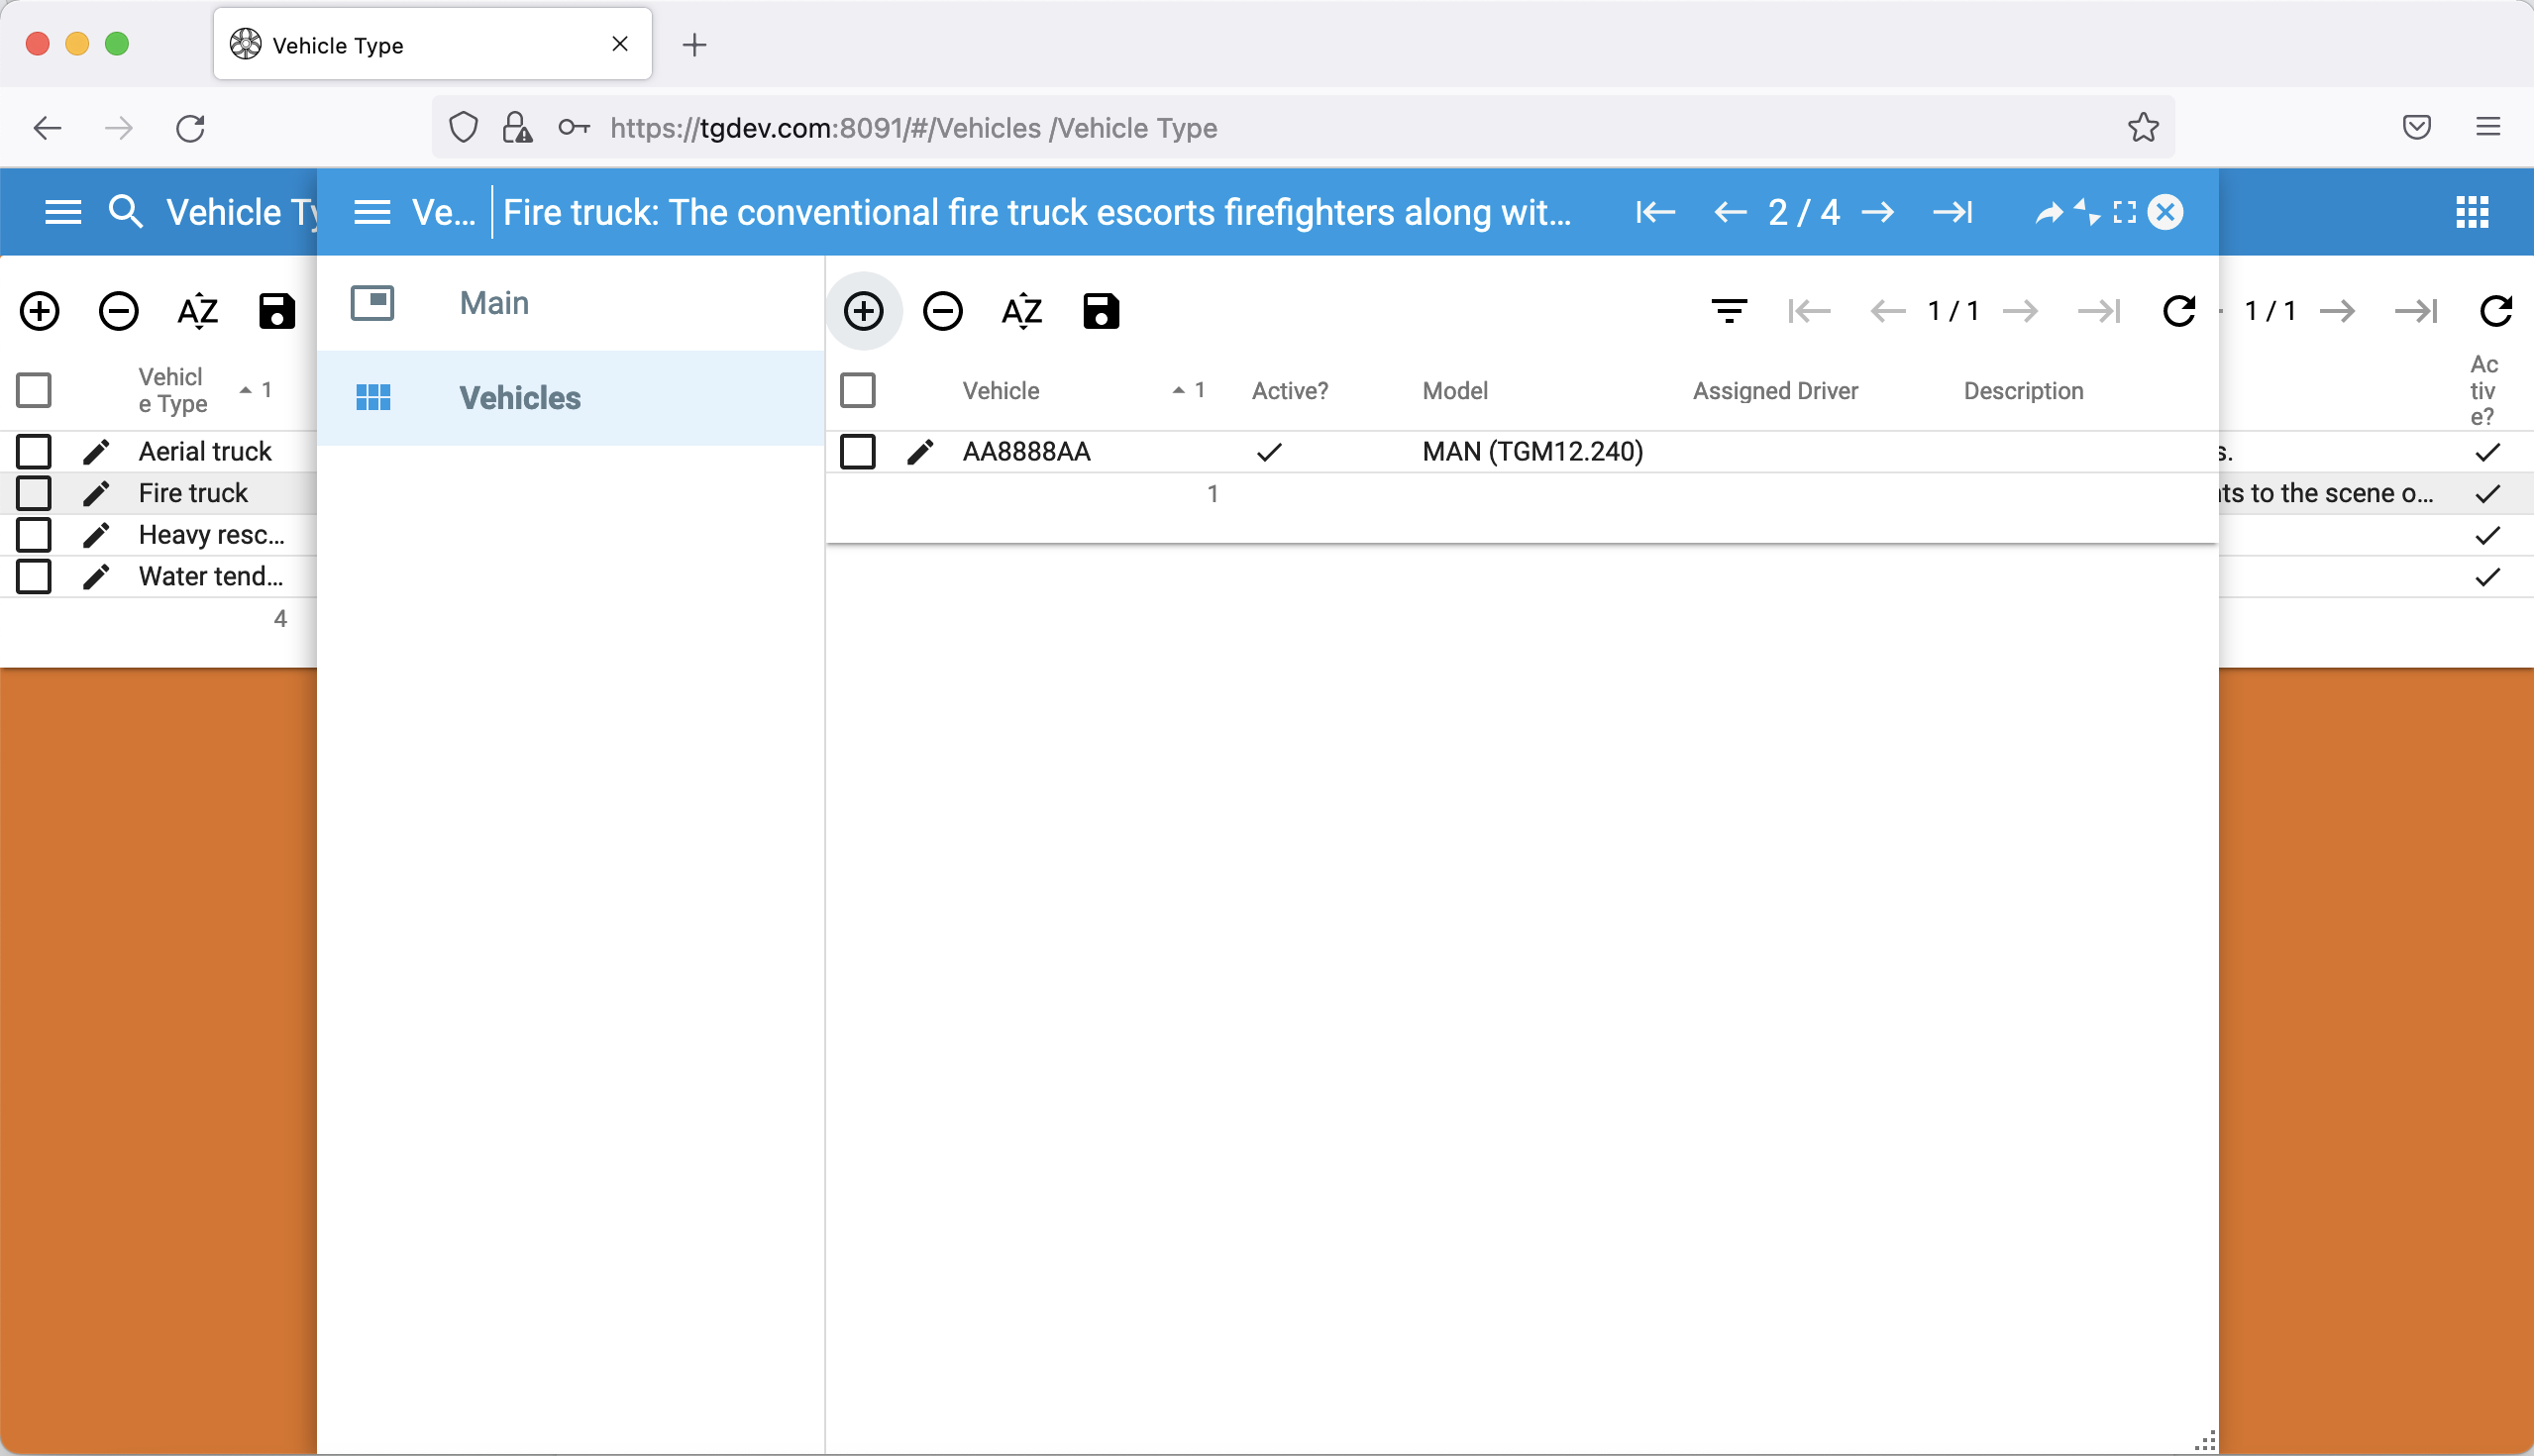
\includegraphics[width=0.95\linewidth]{sections/vehicles/images/24.png}
	\caption{Embedded vehicle search results.}\label{sections/vehicles/images/24}
	\end{figure}

\newpage
Users can also search for existing vehicles related only to this specific vehicle type either by specifying number, which is auto-completed, or activity status, or model, or assigned driver, or description, as displayed on
\hyperref[sections/vehicles/images/25]{Fig.~\ref*{sections/vehicles/images/25}}.

    \begin{figure}[!htbp]
	\centering
	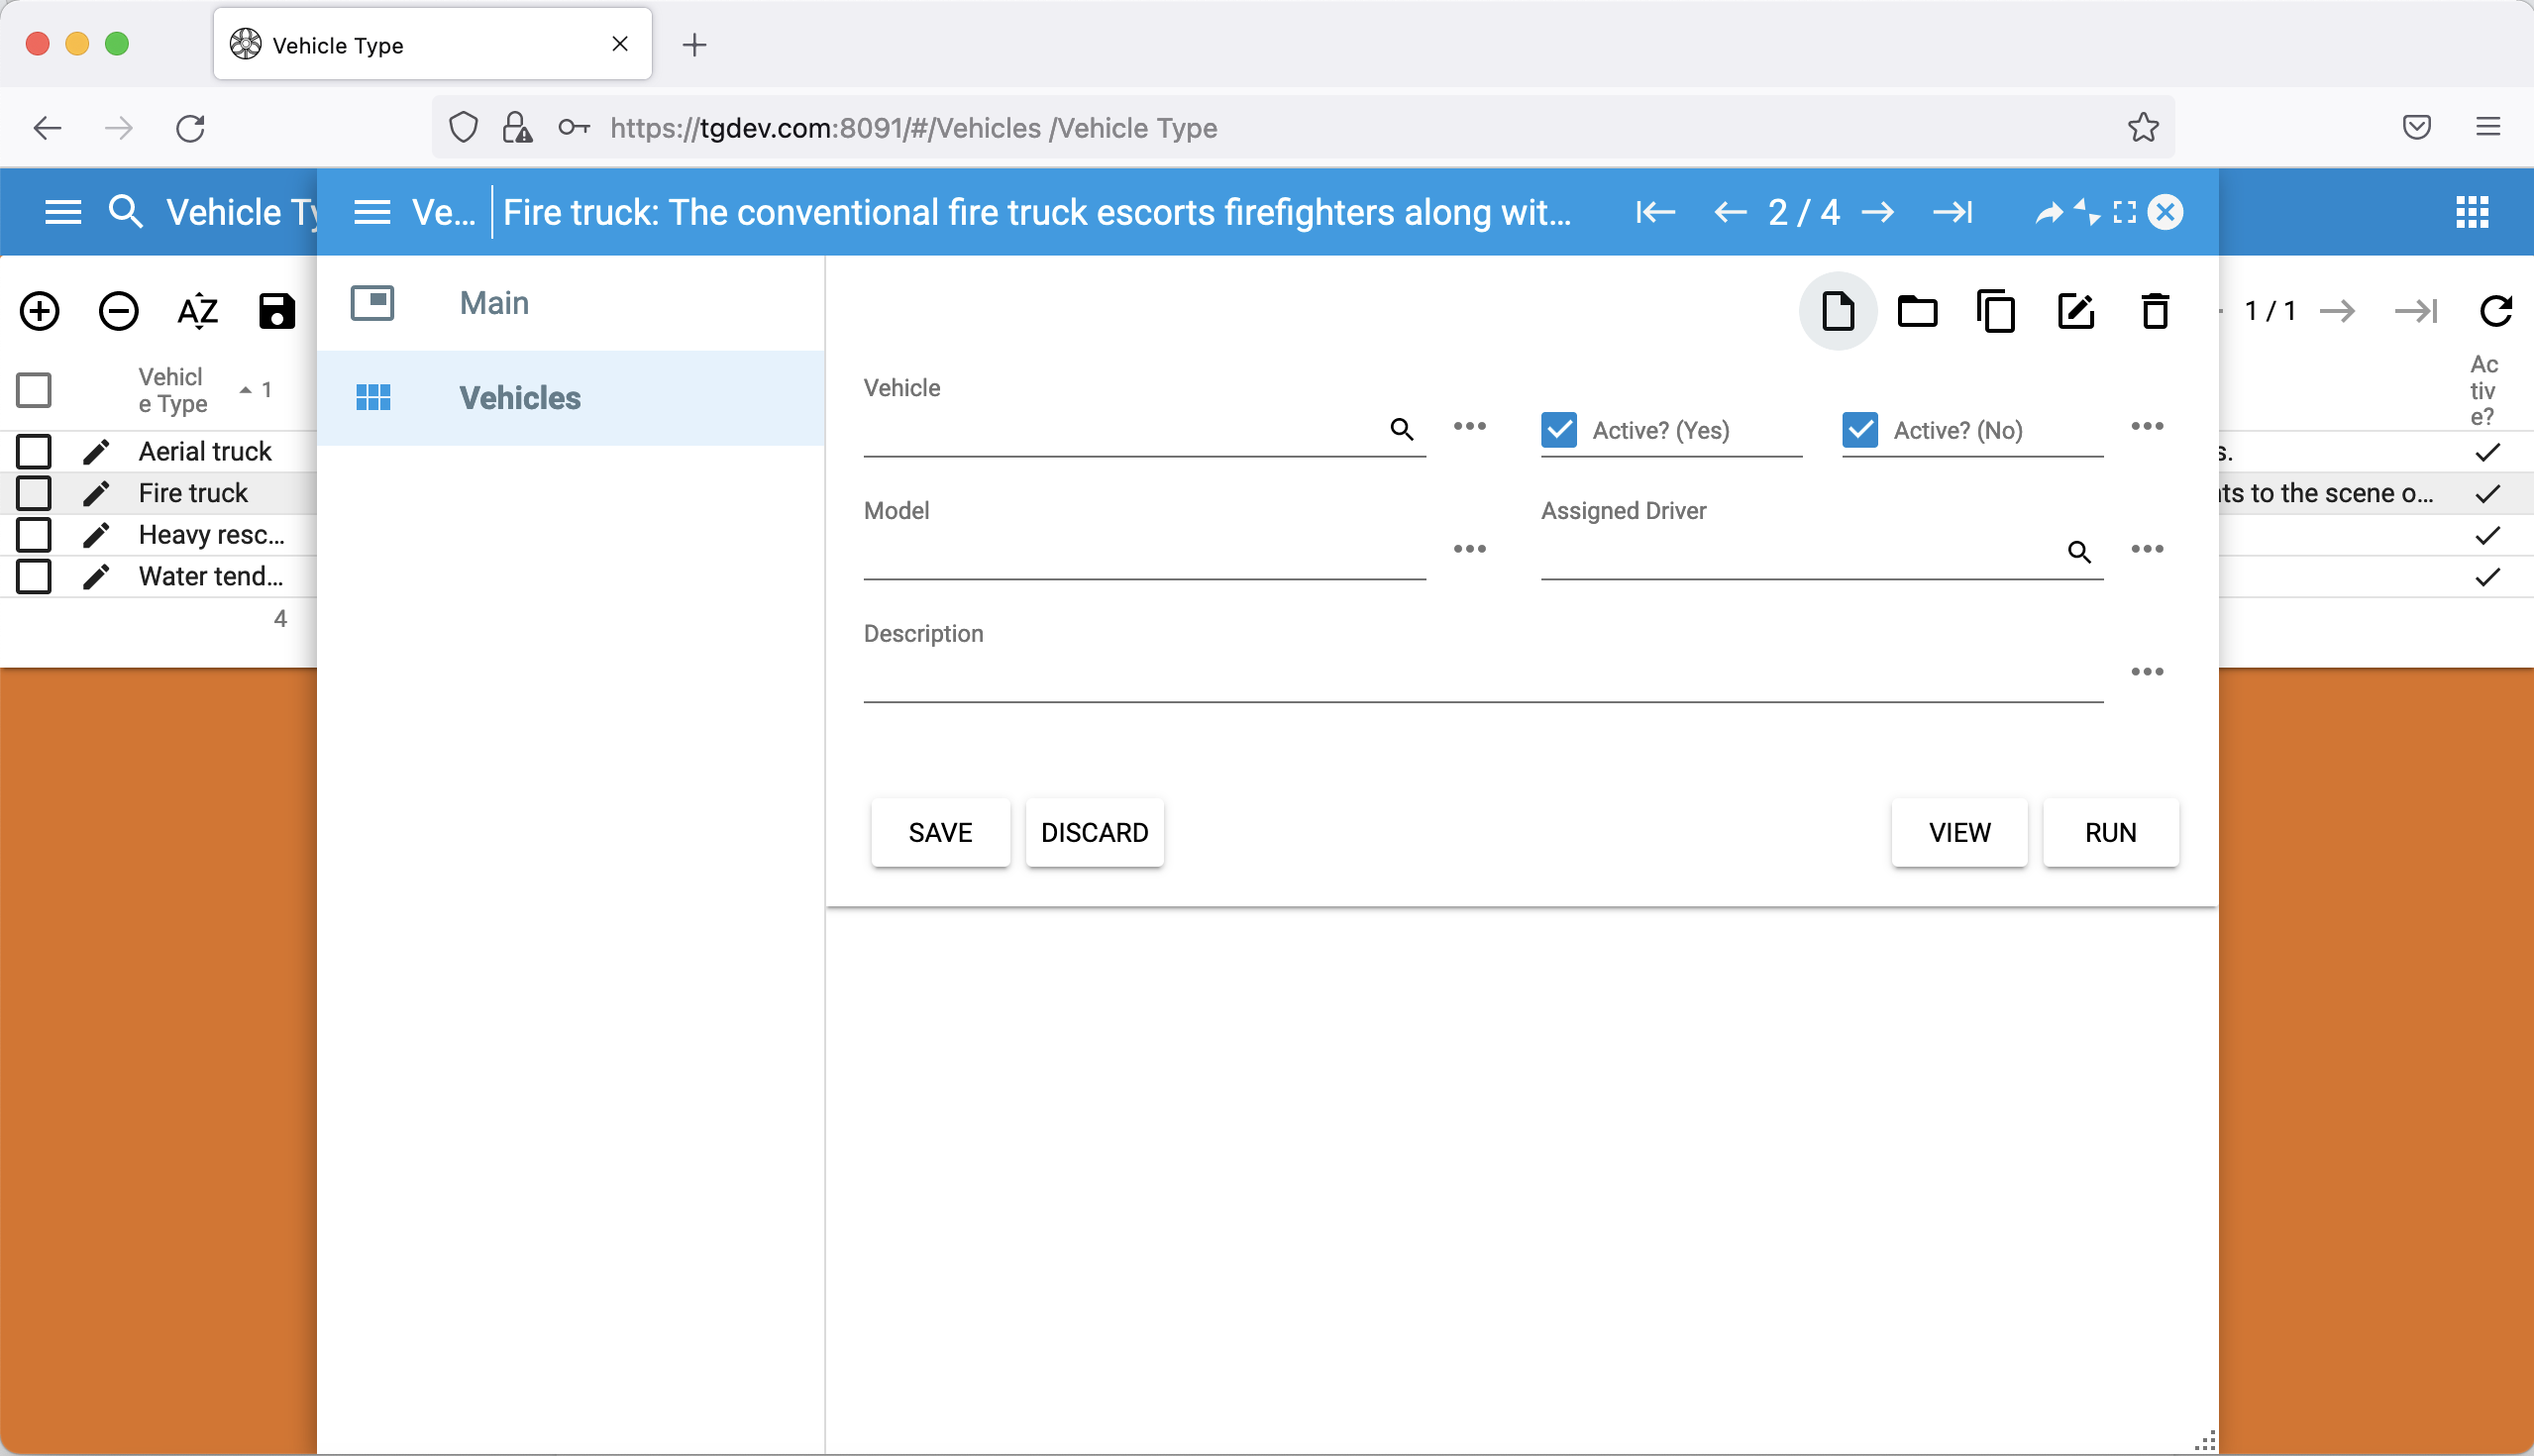
\includegraphics[width=0.95\linewidth]{sections/vehicles/images/25.png}
	\caption{Embedded vehicle search query.}\label{sections/vehicles/images/25}
	\end{figure}
	
\newpage
Users can also create a new vehicle by filling in its number in format AA9999AA and activity status, as well as its model, assigned driver (optional), and description (optional) as displayed on \hyperref[sections/vehicles/images/26]{Fig.~\ref*{sections/vehicles/images/26}}. Vehicle Type field is automatically auto-completed with this specific vehicle type.

    \begin{figure}[!htbp]
	\centering
	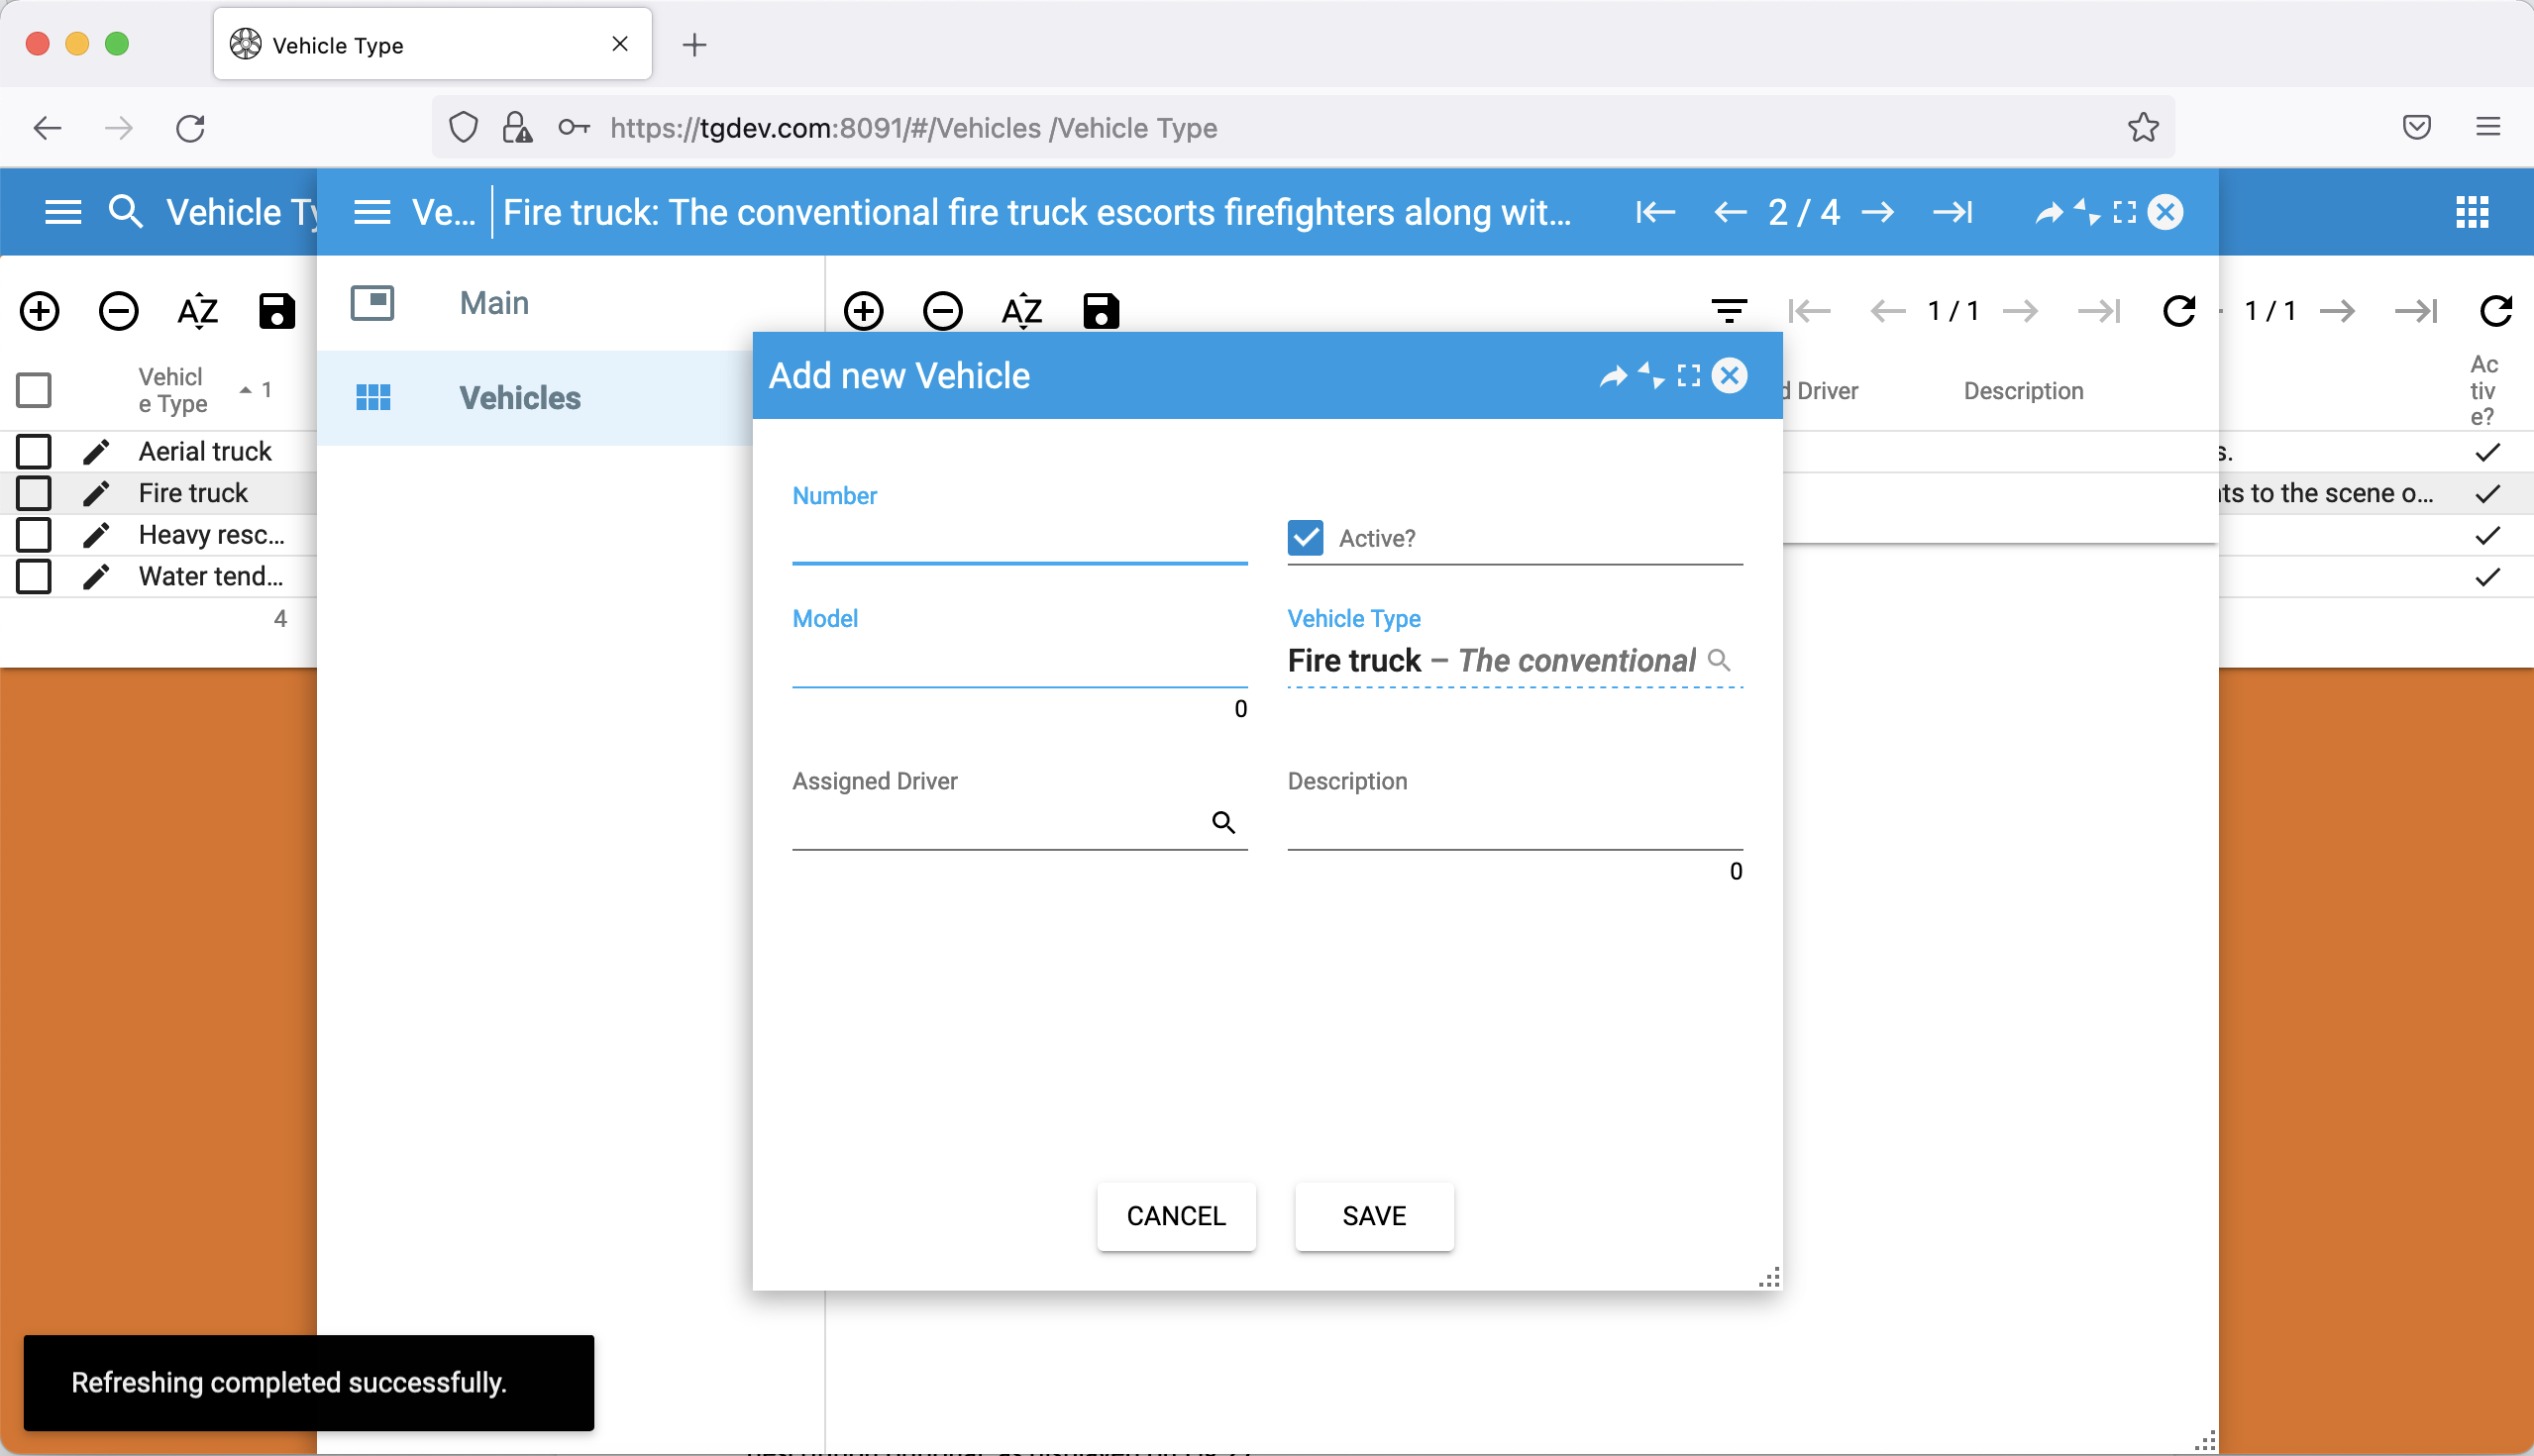
\includegraphics[width=0.95\linewidth]{sections/vehicles/images/26.png}
	\caption{Embedded vehicle creation.}\label{sections/vehicles/images/26}
	\end{figure}

\newpage	
\subsection{Vehicle}
In order to perform registration, classification and tracking of vehicles correctly, users can create vehicles. When creating a new vehicle, users have to fill in its number in format AA9999AA, activity status, corresponding vehicle type which is auto-completed, model, assigned driver (optional), and its description optional, as displayed on \hyperref[sections/vehicles/images/27]{Fig.~\ref*{sections/vehicles/images/27}}.

    \begin{figure}[!htbp]
	\centering
	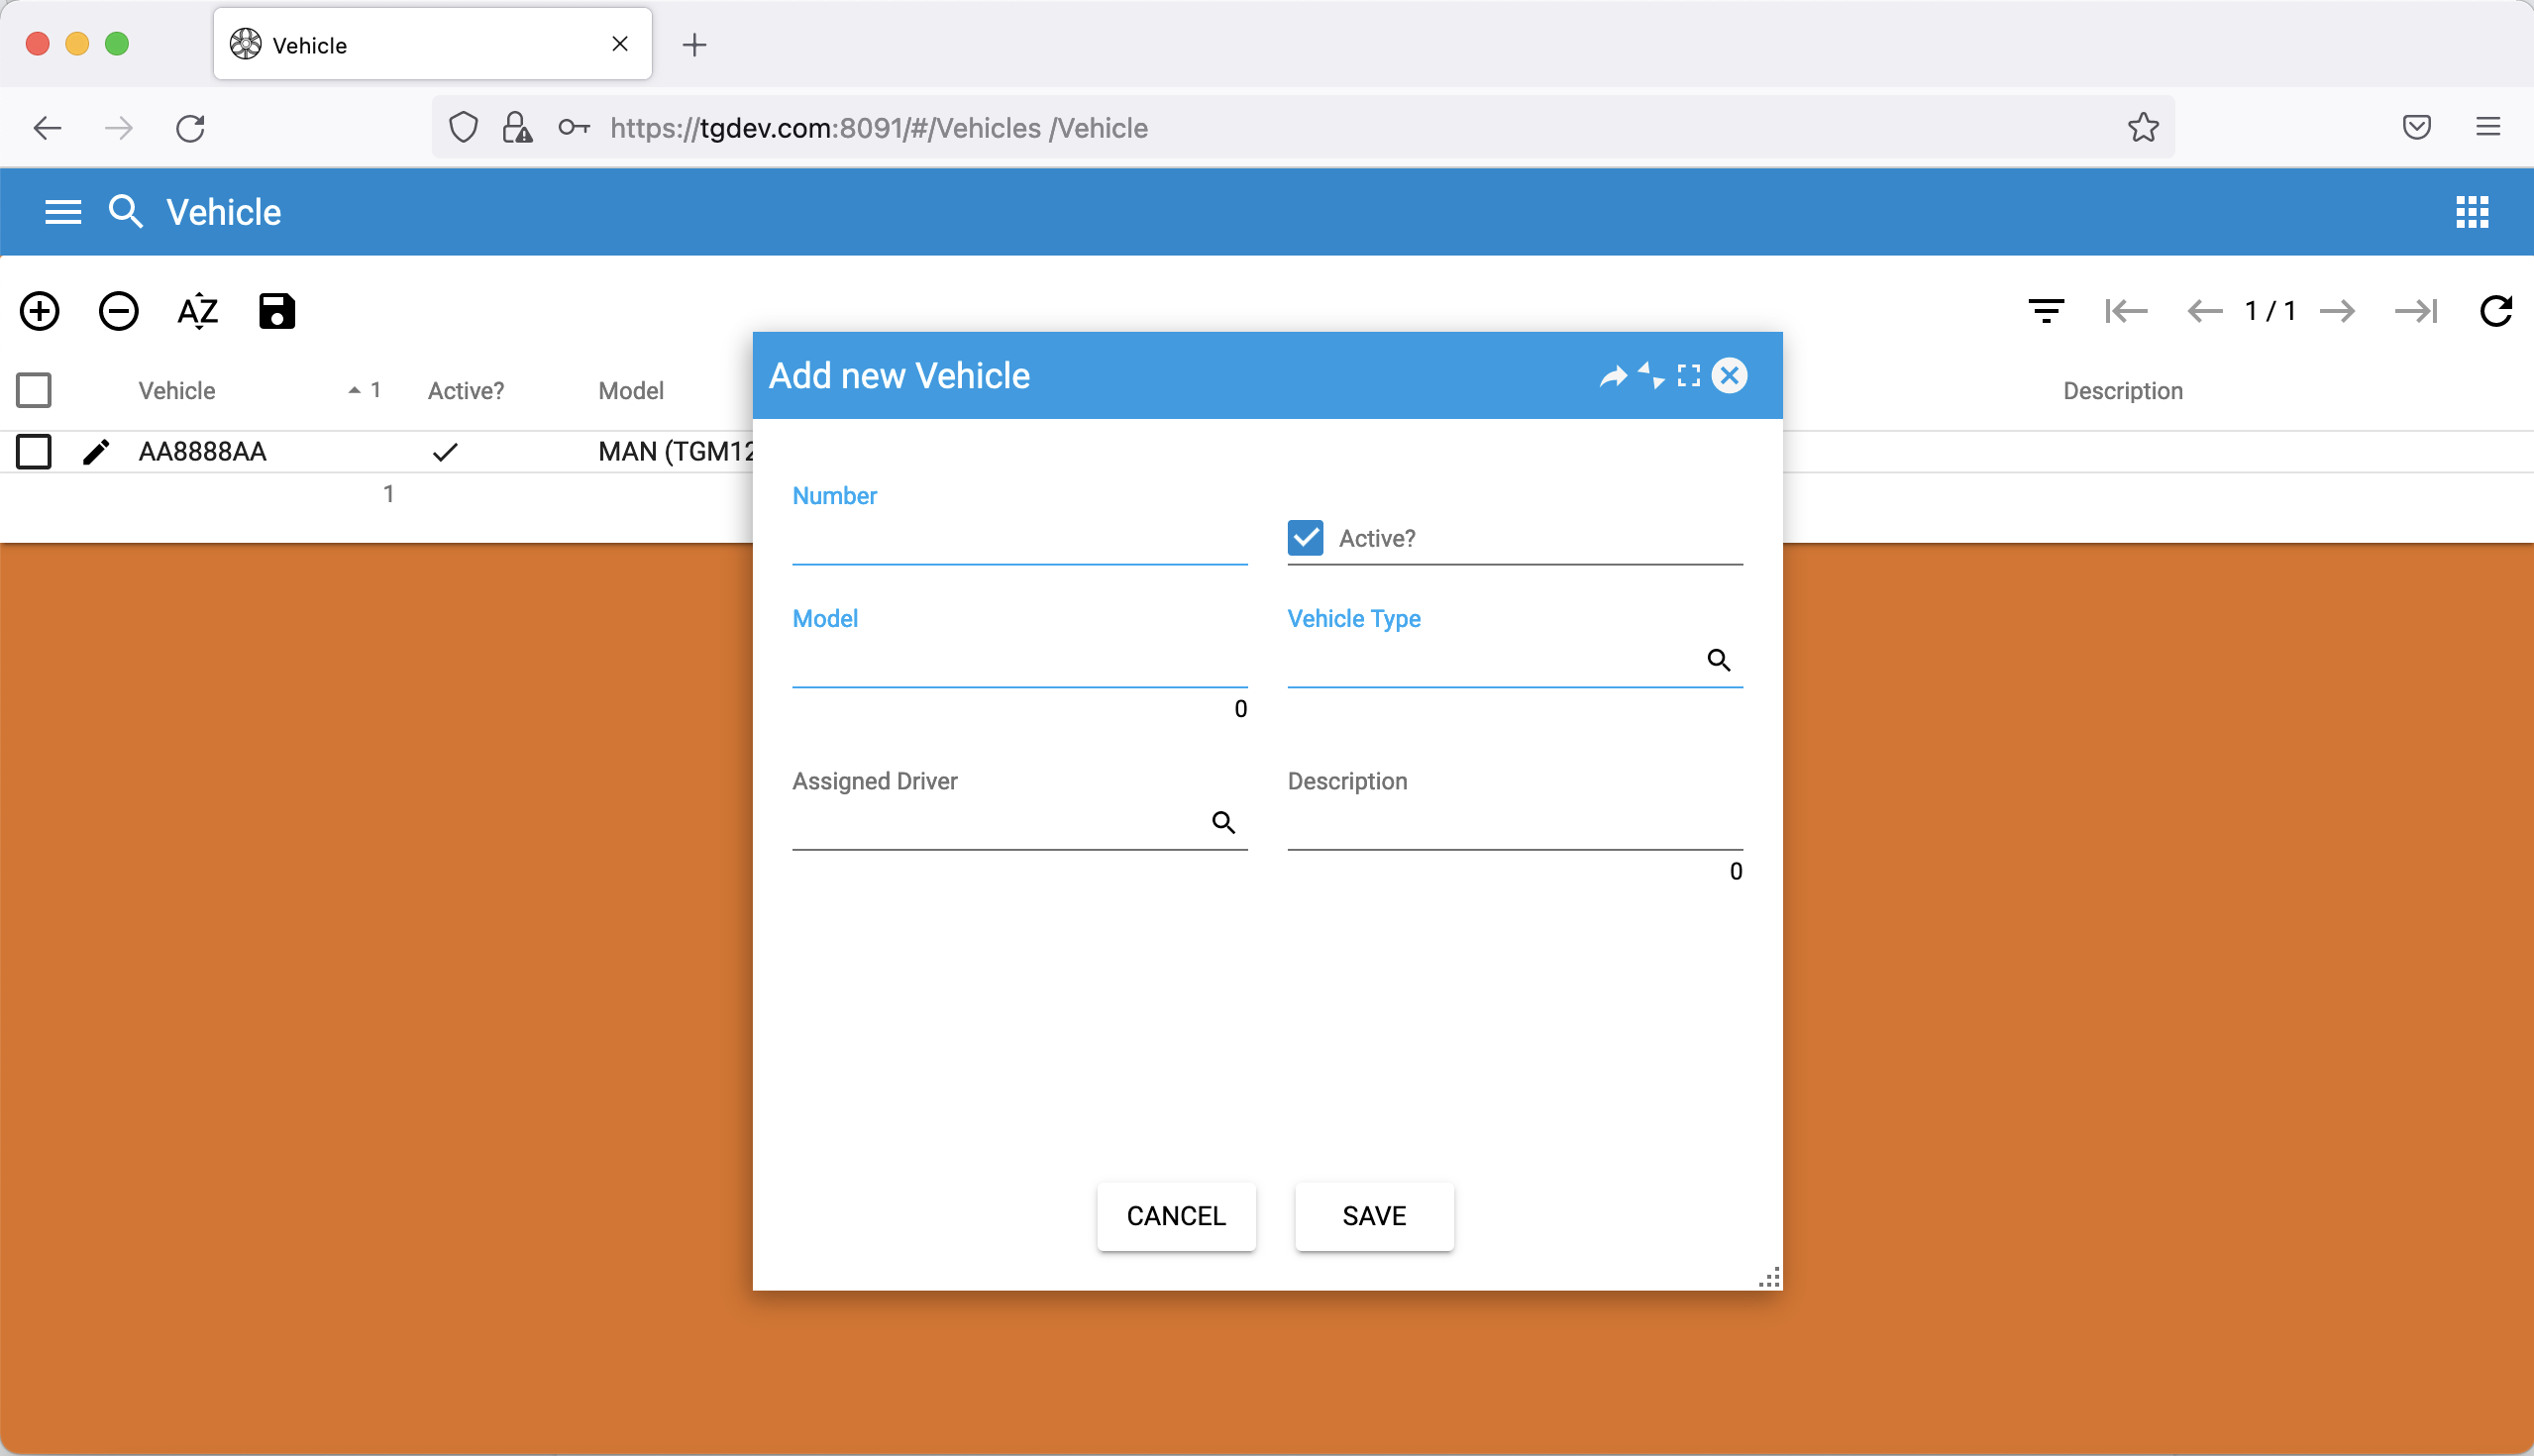
\includegraphics[width=0.95\linewidth]{sections/vehicles/images/27.png}
	\caption{Vehicle creation.}\label{sections/vehicles/images/27}
	\end{figure}

Users can also search for specific vehicles and edit them as described in the vehicle type embedded master section.
    \section{Forms Module}\label{sec:01}

Forms allow users to perform a daily checkup of the equipment, assigned to them. A new Form items can be added in the "Form Item" folder. Forms functionality is currently under development, but it will contain a Collection of the "Form Items". A User can change the status (Accepted or not) of the Form Item on the Form Class web page. Every Form has the Status property, that can be created and modified in the "Users and Personnel" module.

\subsection{Form Item}
In order for the Item to be shown in he form, it must be created on the Form Item page with the following properties: \textbf{Accepted} and \textbf{Form Type Item}.

    \begin{figure}[!htbp]
    \centering
    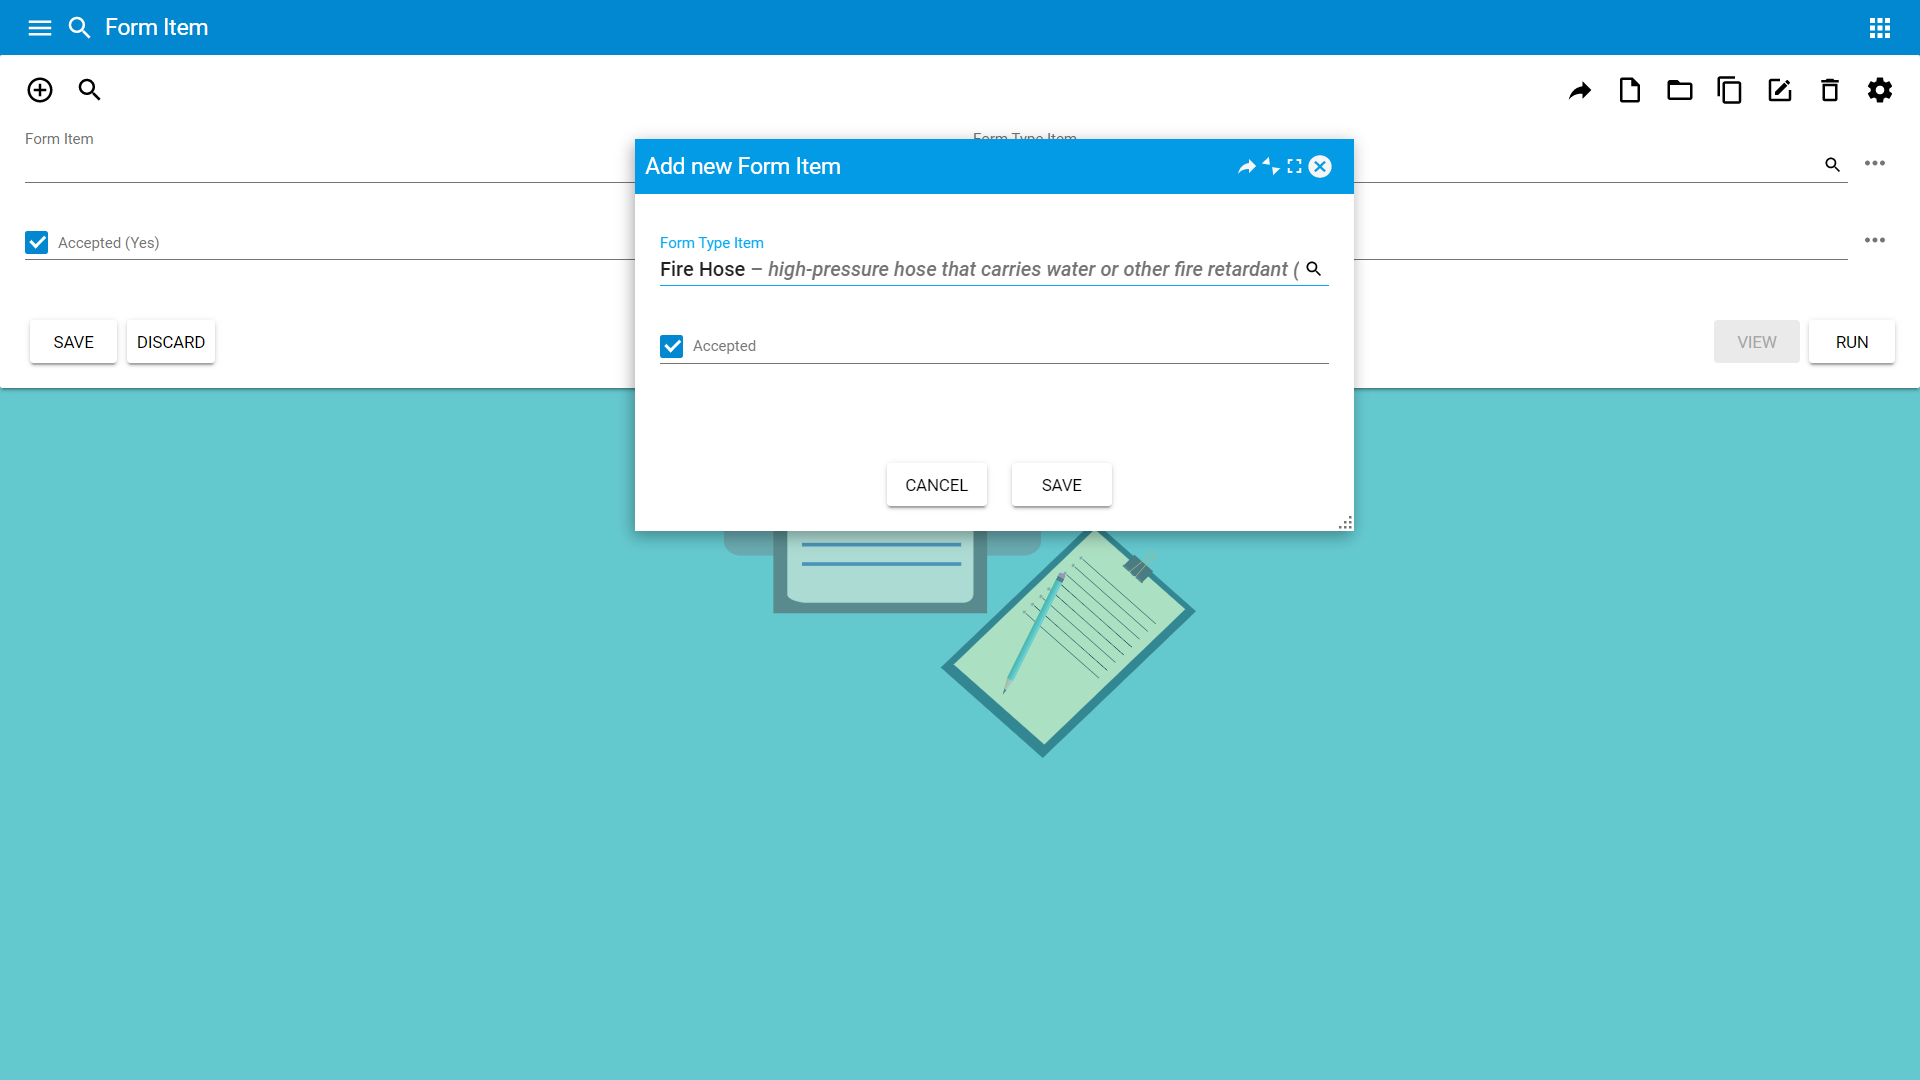
\includegraphics[width=0.95\linewidth]{sections/forms/images/add_new_form_item.png}
    \caption{Form Item creation.}\label{sections/forms/images/add_new_form_item}
    \end{figure}

Users can perform search operation for the form items based on their \textbf{Accepted} status or \textbf{Form Type Item} field.
\newpage

\subsection{Form Type Item}
\textbf{Form Type Item} is a base class for the \textbf{Form Item} creation. Many Form Items can be created from one Form Type Item. 

Form Type Item has the unique Title (without white spaces) and Description fields. For example, a new Form Type Item can be: "\textbf{Title:} \textit{Fire Gloves}; \textbf{Description}: \textit{Important part of the personal protection equipment}."  

% \hyperref[sections/equipment/images/Fig.3]{Fig.~\ref*{sections/equipment/images/Fig.3}}.

    \begin{figure}[!htbp]
	\centering
	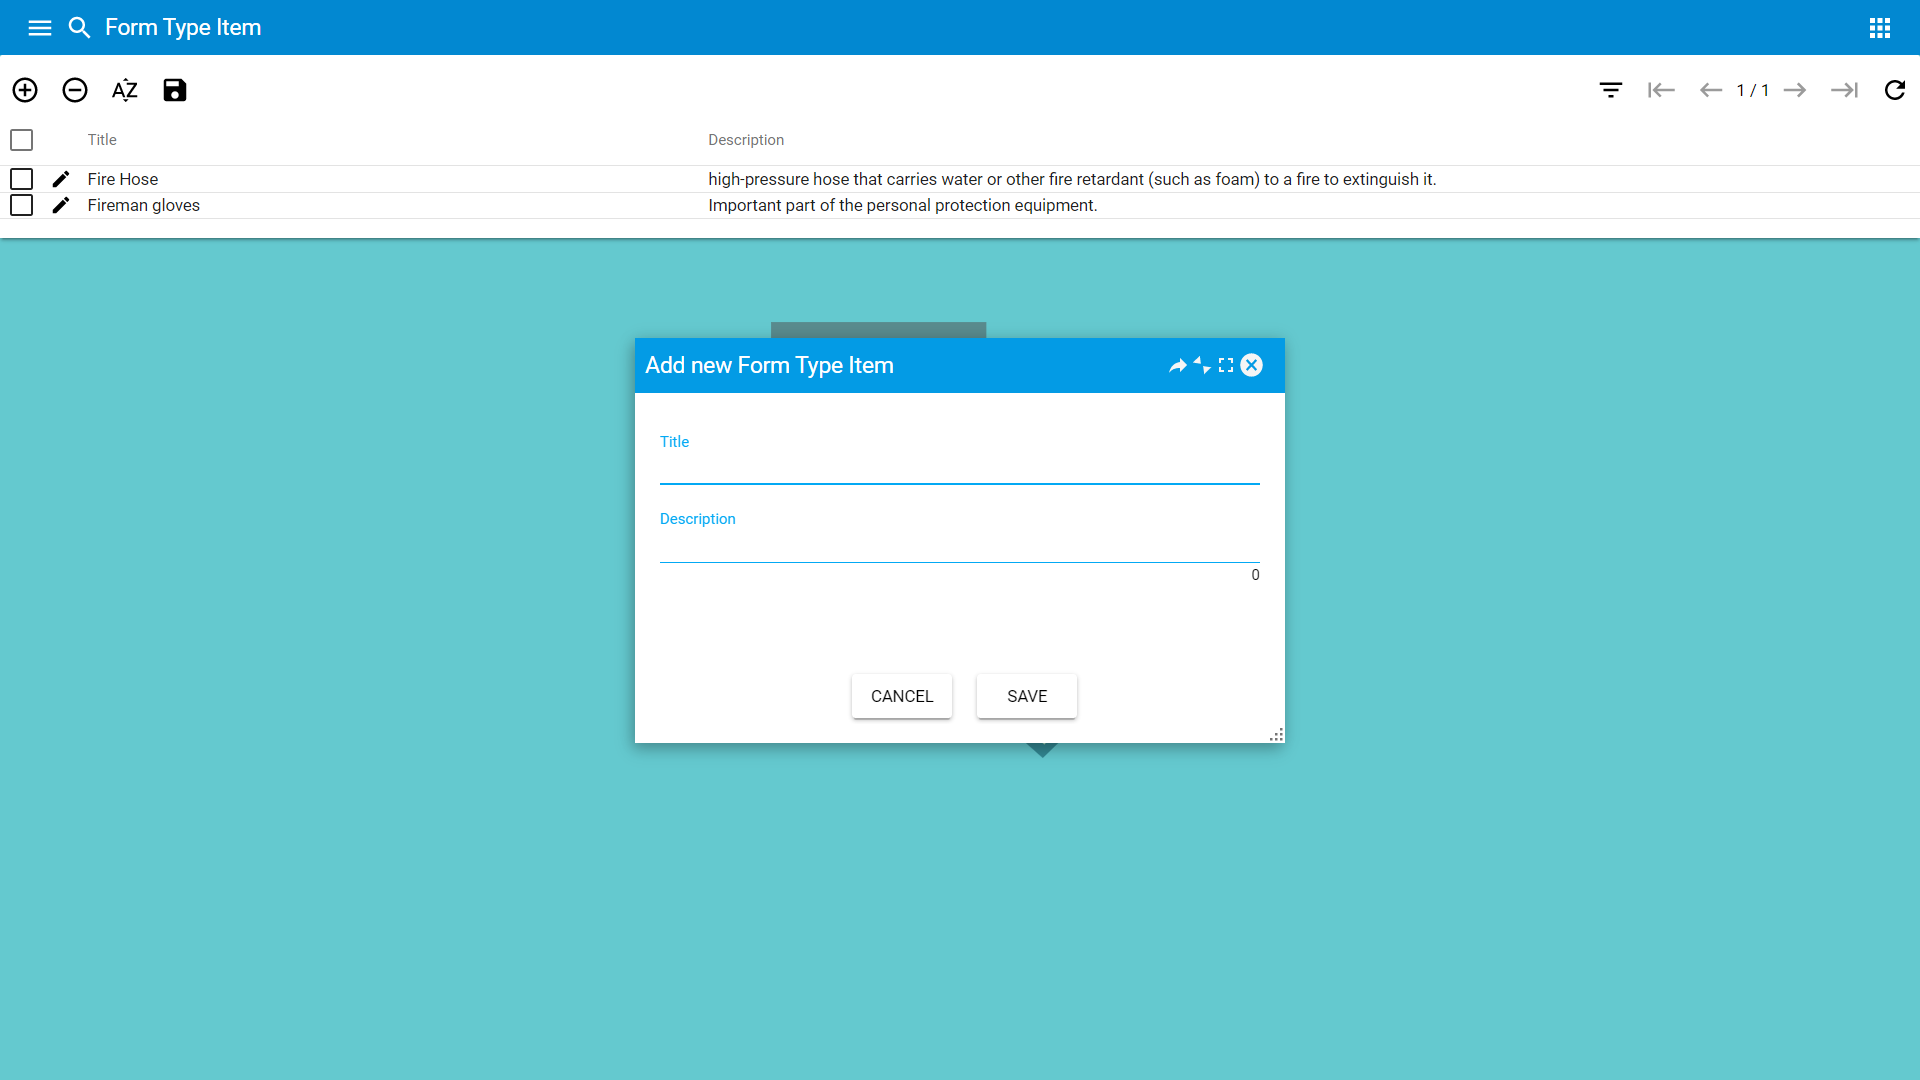
\includegraphics[width=0.95\linewidth]{sections/forms/images/add_newform_type_item.png}
	\caption{Form Type Item creation.}\label{sections/forms/images/add_newform_type_item}
	\end{figure}

Users can perform search operation for the form type items based on their \textbf{Title} or \textbf{Description} values.
\newpage

\subsection{Form Type}
The \textbf{Form Type} is currently under development. 

\textbf{Form Type} is a tool to use the Forms and update the Form Items' statuses. For example, manager Andriy created the Form Type that can be assigned to employee with a specific role, for example Vehicle Driver. Then all the employee with Vehicle Driver role will have the permission to update current form in order to track the status of the equipment during the daily checkup. 

For now, the Form has the unique \textbf{Title} name, \textbf{Assigned Role},  \textbf{Form Class} and \textbf{Description} fields. It is expected that on the next release there will be N additional fields representing status of the Form Items, that can be updated by workers with the specified role.

\begin{figure}[!htbp]
\centering
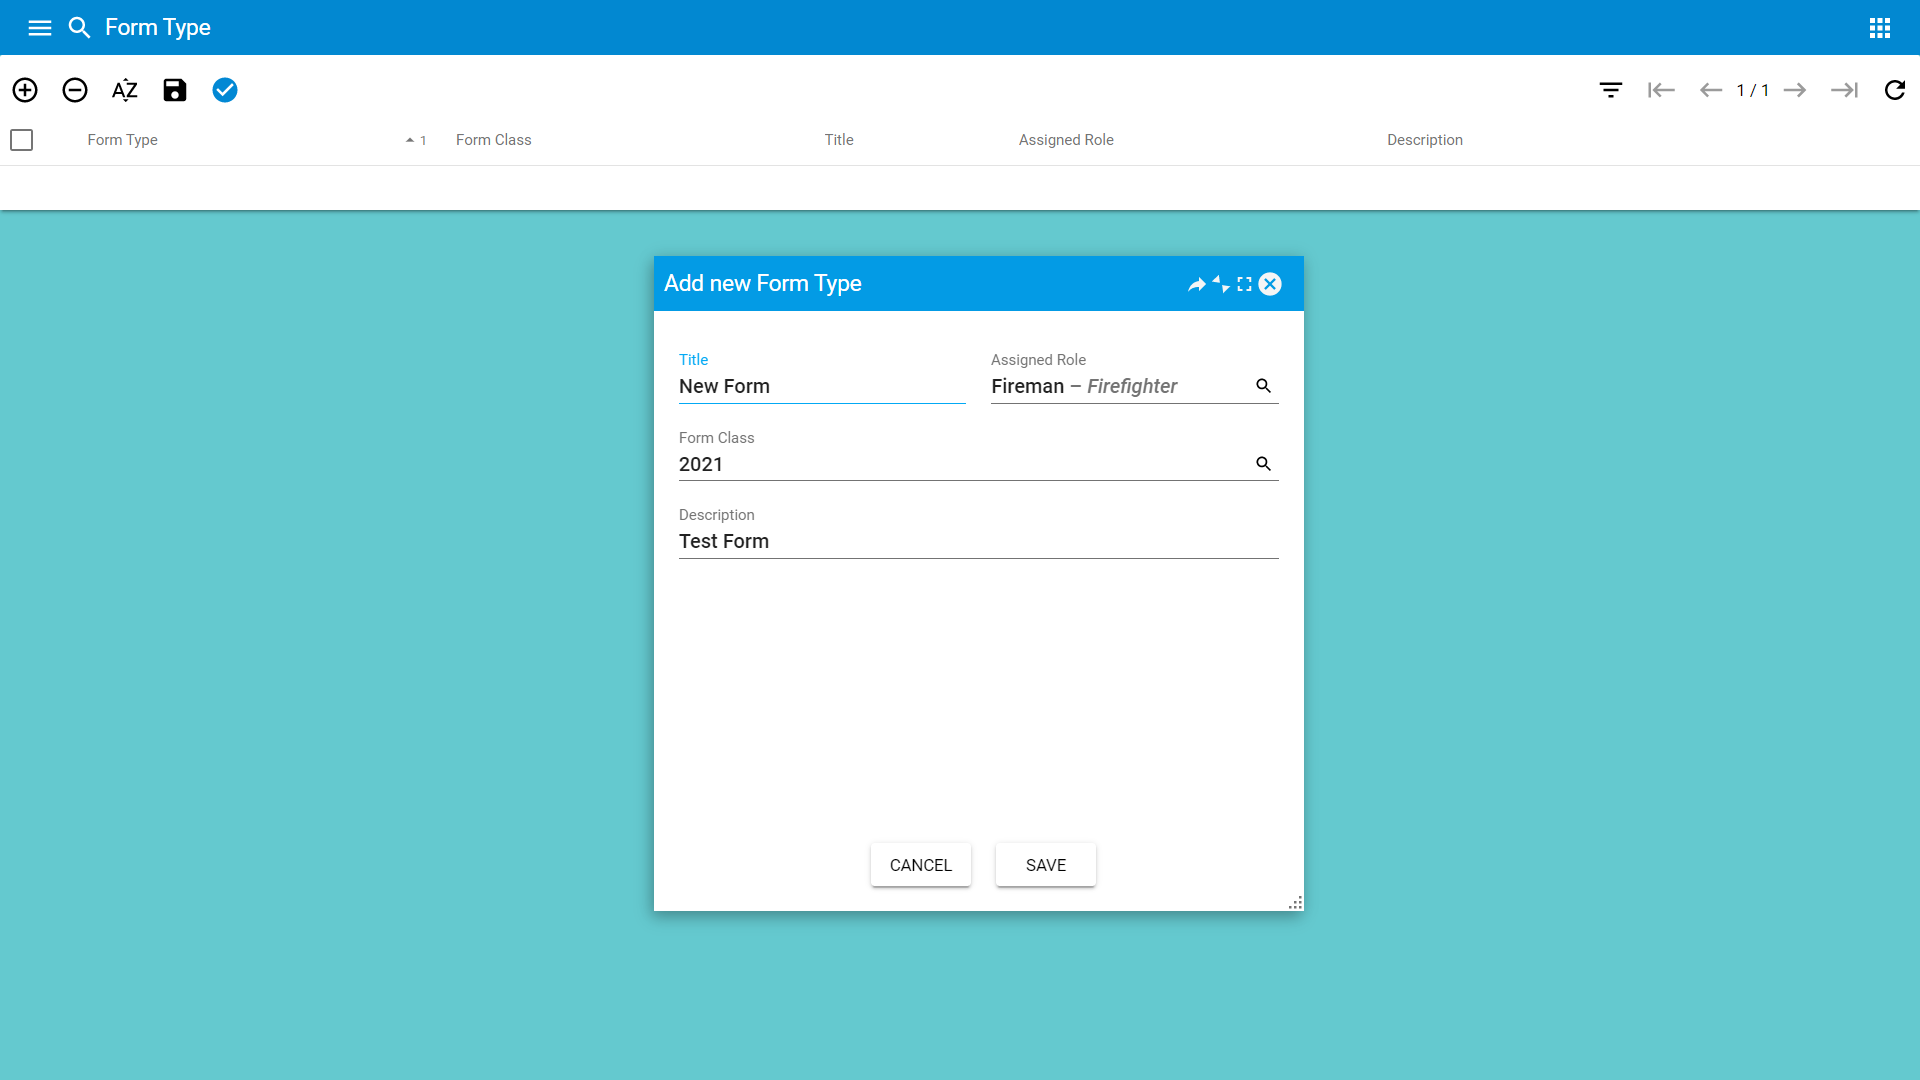
\includegraphics[width=0.95\linewidth]{sections/forms/images/form_type_master.png}
\caption{Form Type creation.}\label{sections/forms/images/form_type_master}
\end{figure}

\newpage
Form Type search query can be used to filter the existing form types, and then to delete or update them. 
\begin{figure}[!htbp]
\centering
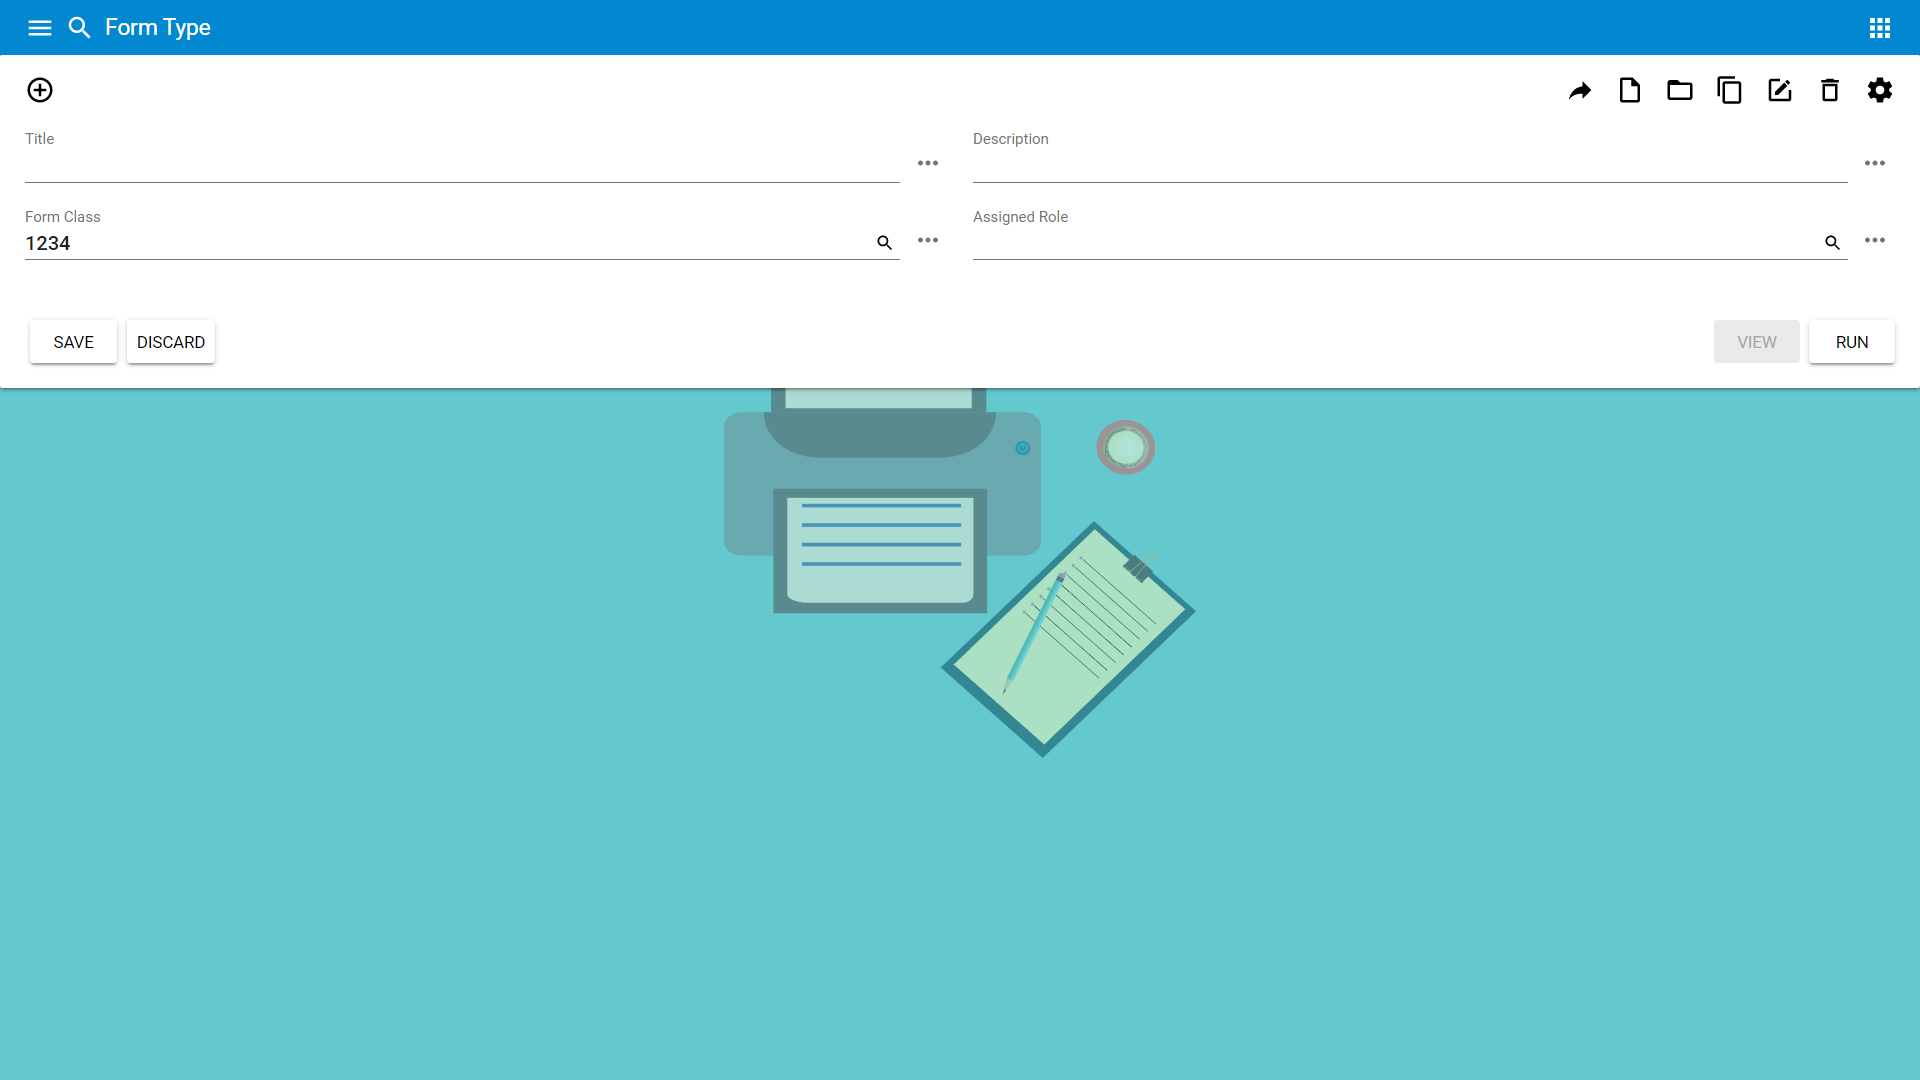
\includegraphics[width=0.95\linewidth]{sections/forms/images/form_type_centre.png}
\caption{Form Type search query.}\label{sections/forms/images/form_type_centre}
\end{figure}

For the next release, it is also planned to correctly fine-tune the BatchUpdate action on the Form Type page. After running the Search query, you can see the checkbox circle on the top of the Form Type page. This is the BatchUpdate action. It updates the status of multiple Form Type entities at once. \textit{You need to select at least one row to perform this action}.

\begin{figure}[!htbp]
\centering
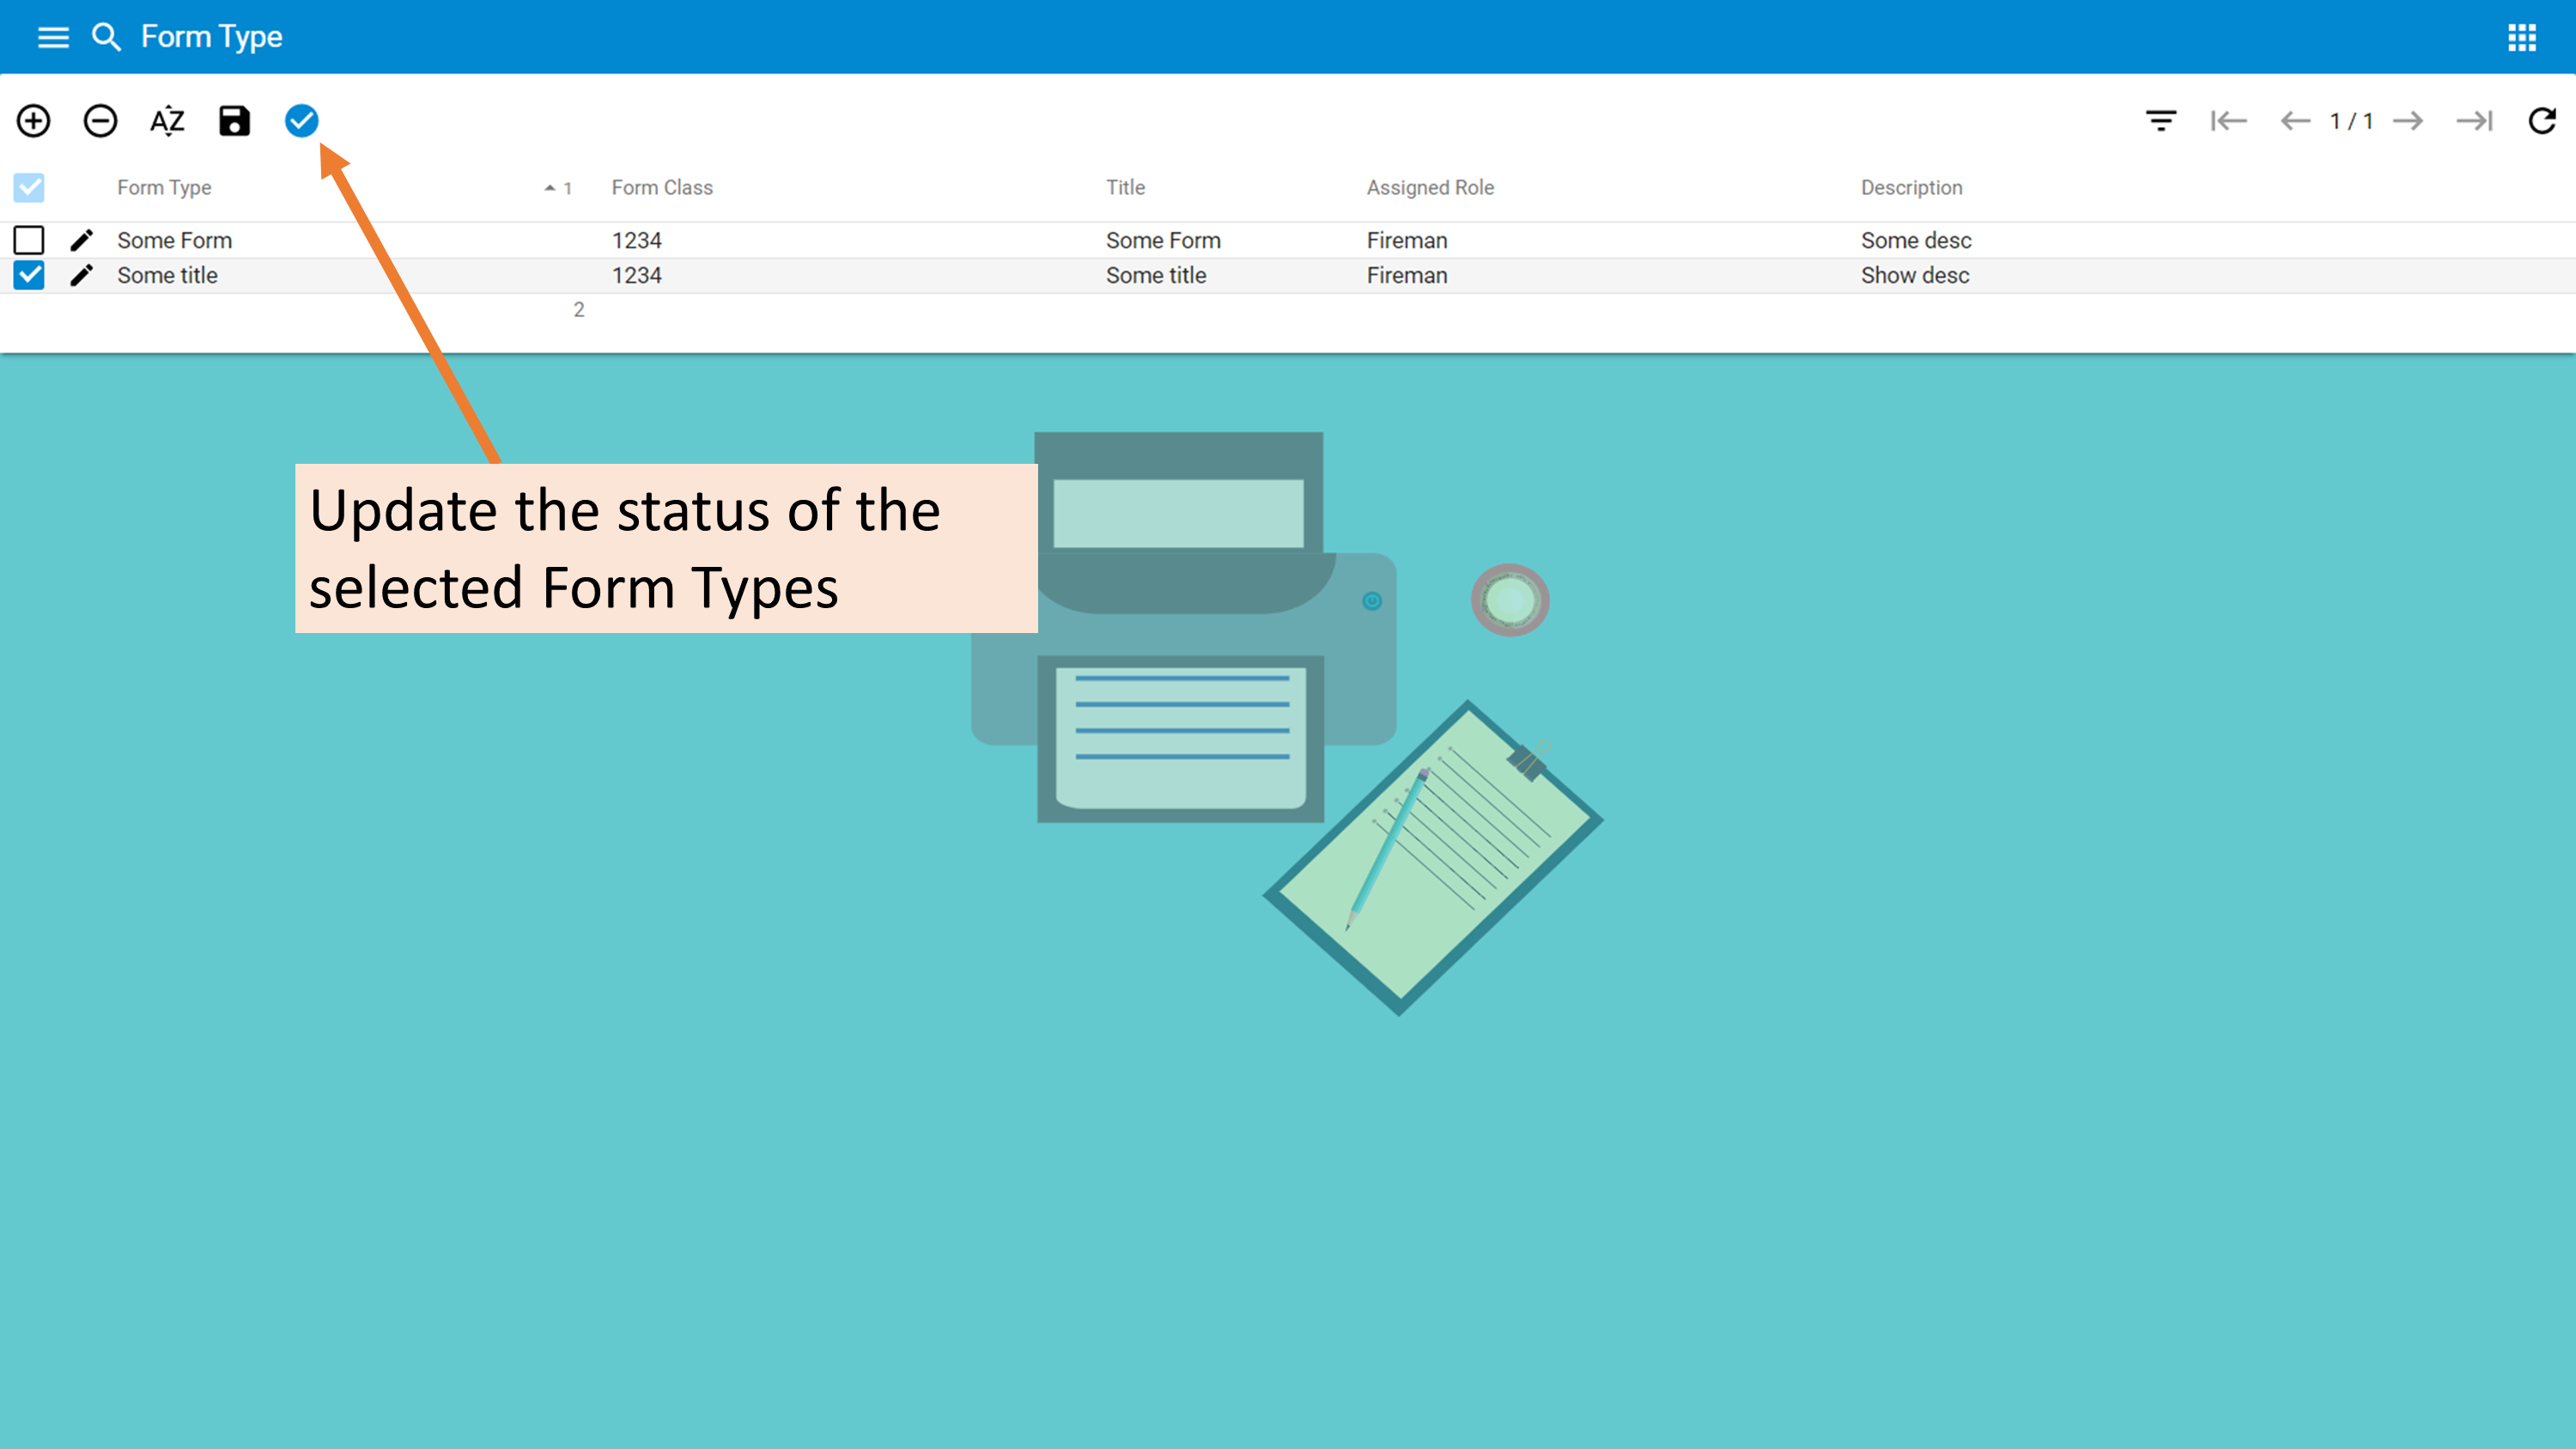
\includegraphics[width=0.95\linewidth]{sections/forms/images/form_type-batch_update.png}
\caption{Form Type Batch Update.}\label{sections/forms/images/form_type-batch_update}
\end{figure}


\newpage

\subsection{Form Class}
Form Class is a tool to create the Forms that will be deployed for everyday use. For example, a worker Andriy created the Form that can be approved by other employees. The Form has the autogenerated name, Status, Date created and Person that is responsible for this form.

\begin{figure}[!htbp]
\centering
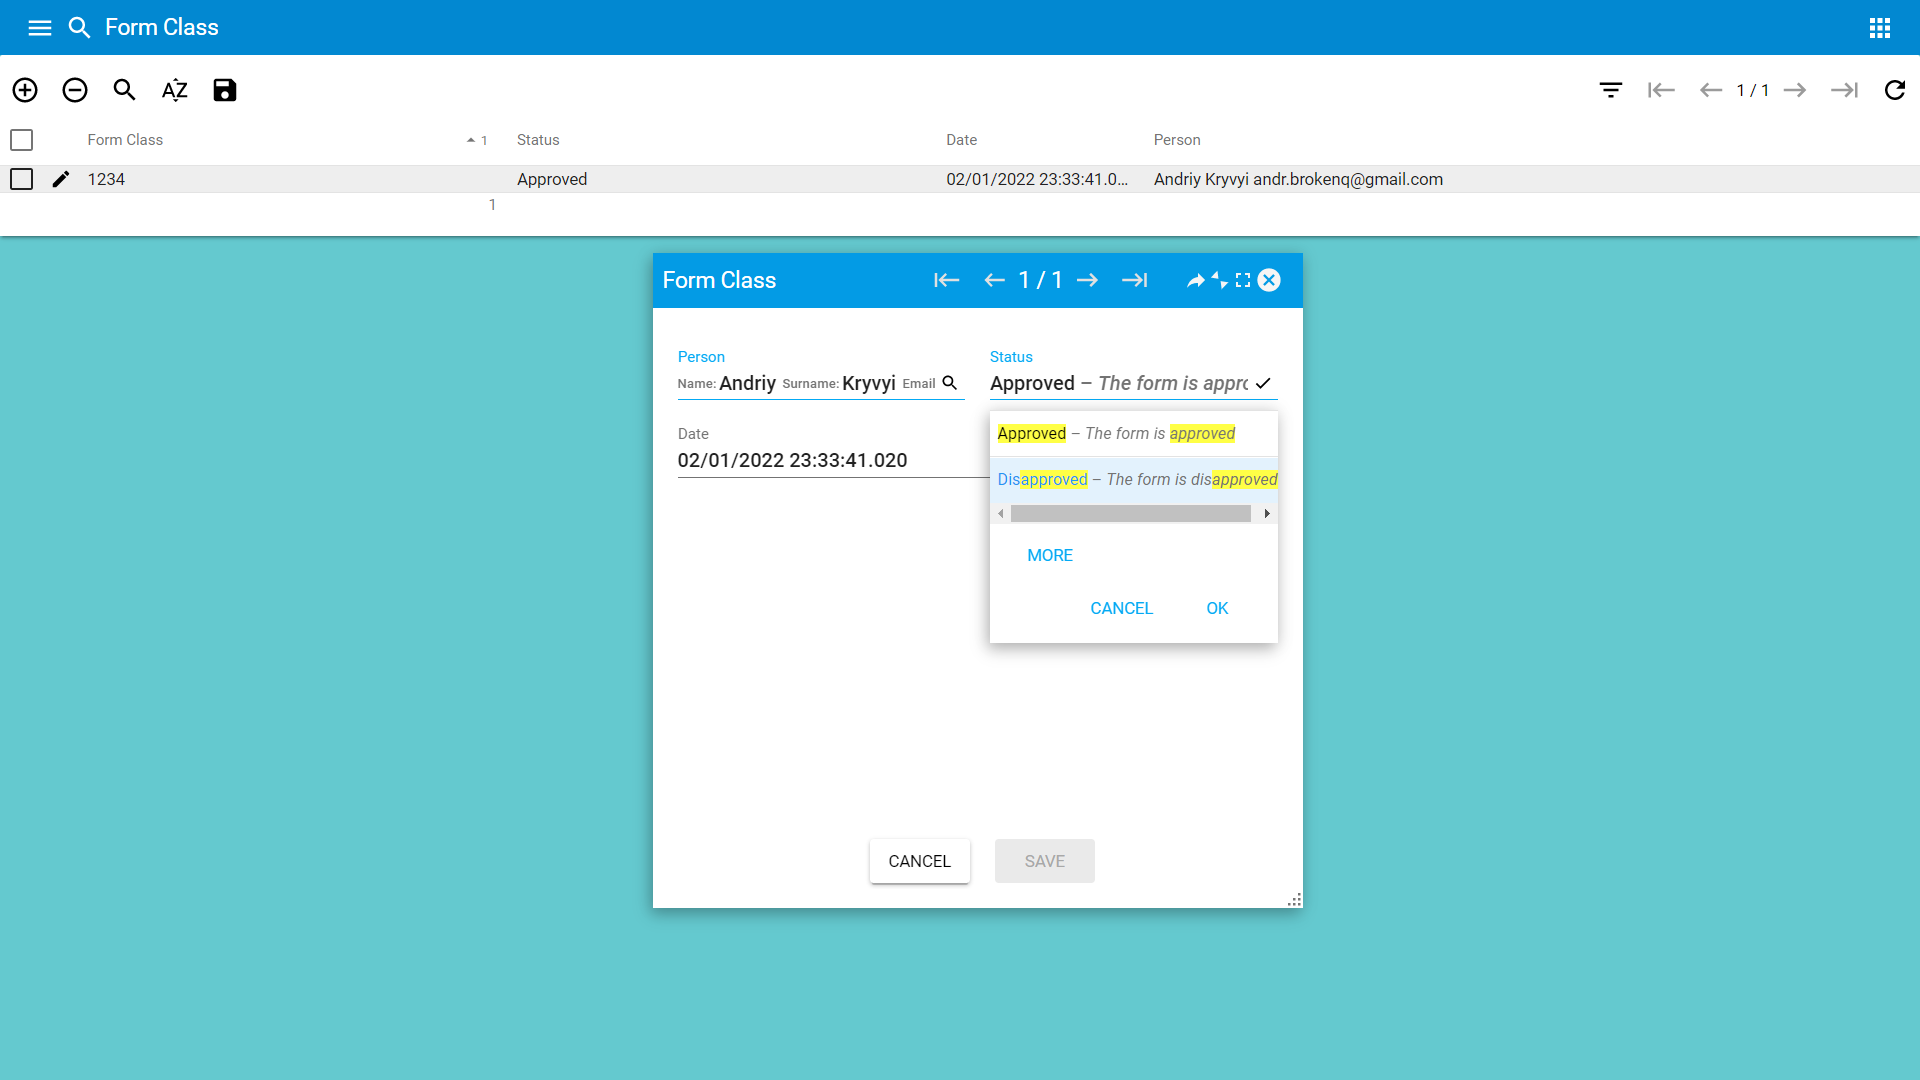
\includegraphics[width=0.95\linewidth]{sections/forms/images/form_class_master.png}
\caption{Form creation.}\label{sections/forms/images/form_class_master}
\end{figure}

Form search query can be used to filter the existing forms, and then delete or update them. 
\begin{figure}[!htbp]
\centering
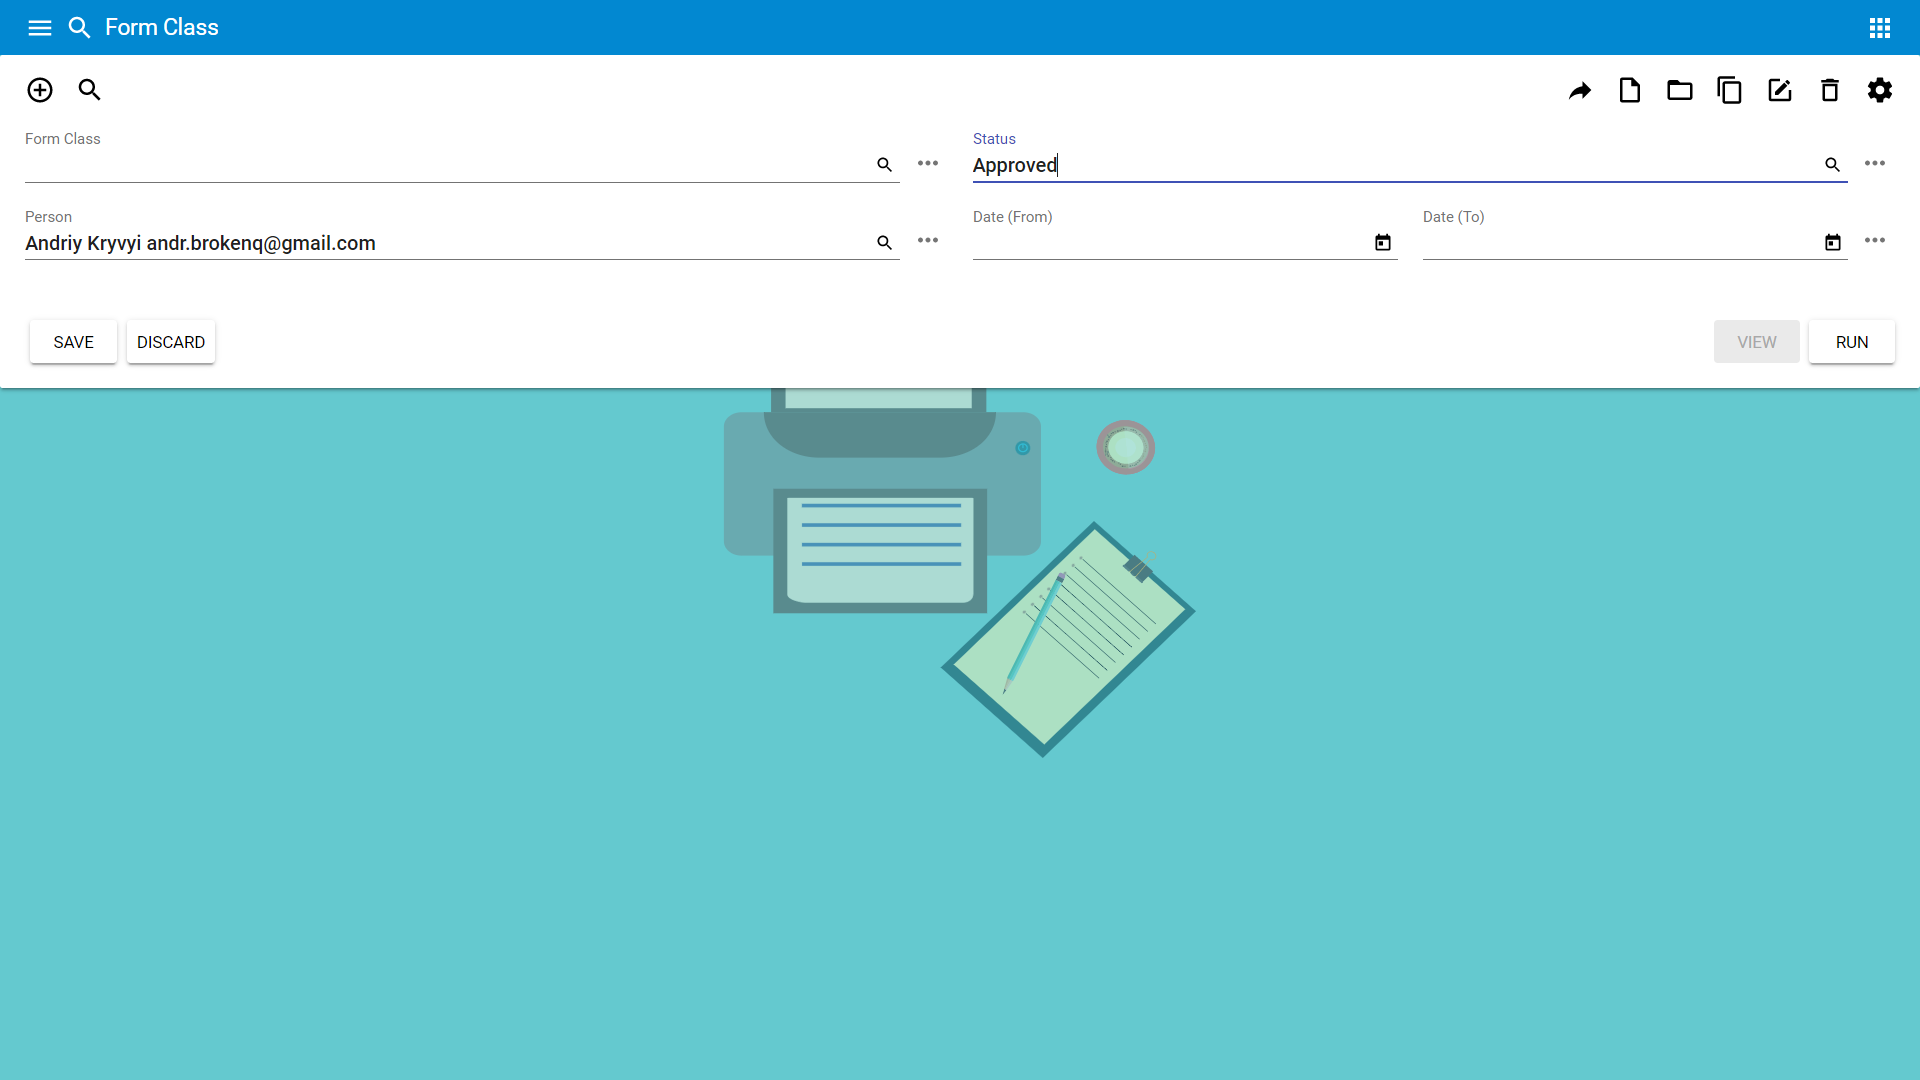
\includegraphics[width=0.95\linewidth]{sections/forms/images/form_class_centre.png}
\caption{Form search query.}\label{sections/forms/images/form_class_centre}
\end{figure}
\newpage


    \section{Users and personnel Module}\label{sec:01}
\subsection{Status}

In order for the fire department captain to review filled forms, he can create different statuses and assign them to these forms. Possible statuses are approved, disapproved, sent for review, etc. When creating a new status, the fire department captain has to fill in the name of the status with no whitespaces and description, as displayed on
\hyperref[sections/personnel/images/16]{Fig.~\ref*{sections/personnel/images/16}}.

\begin{figure}[!htbp]
\centering
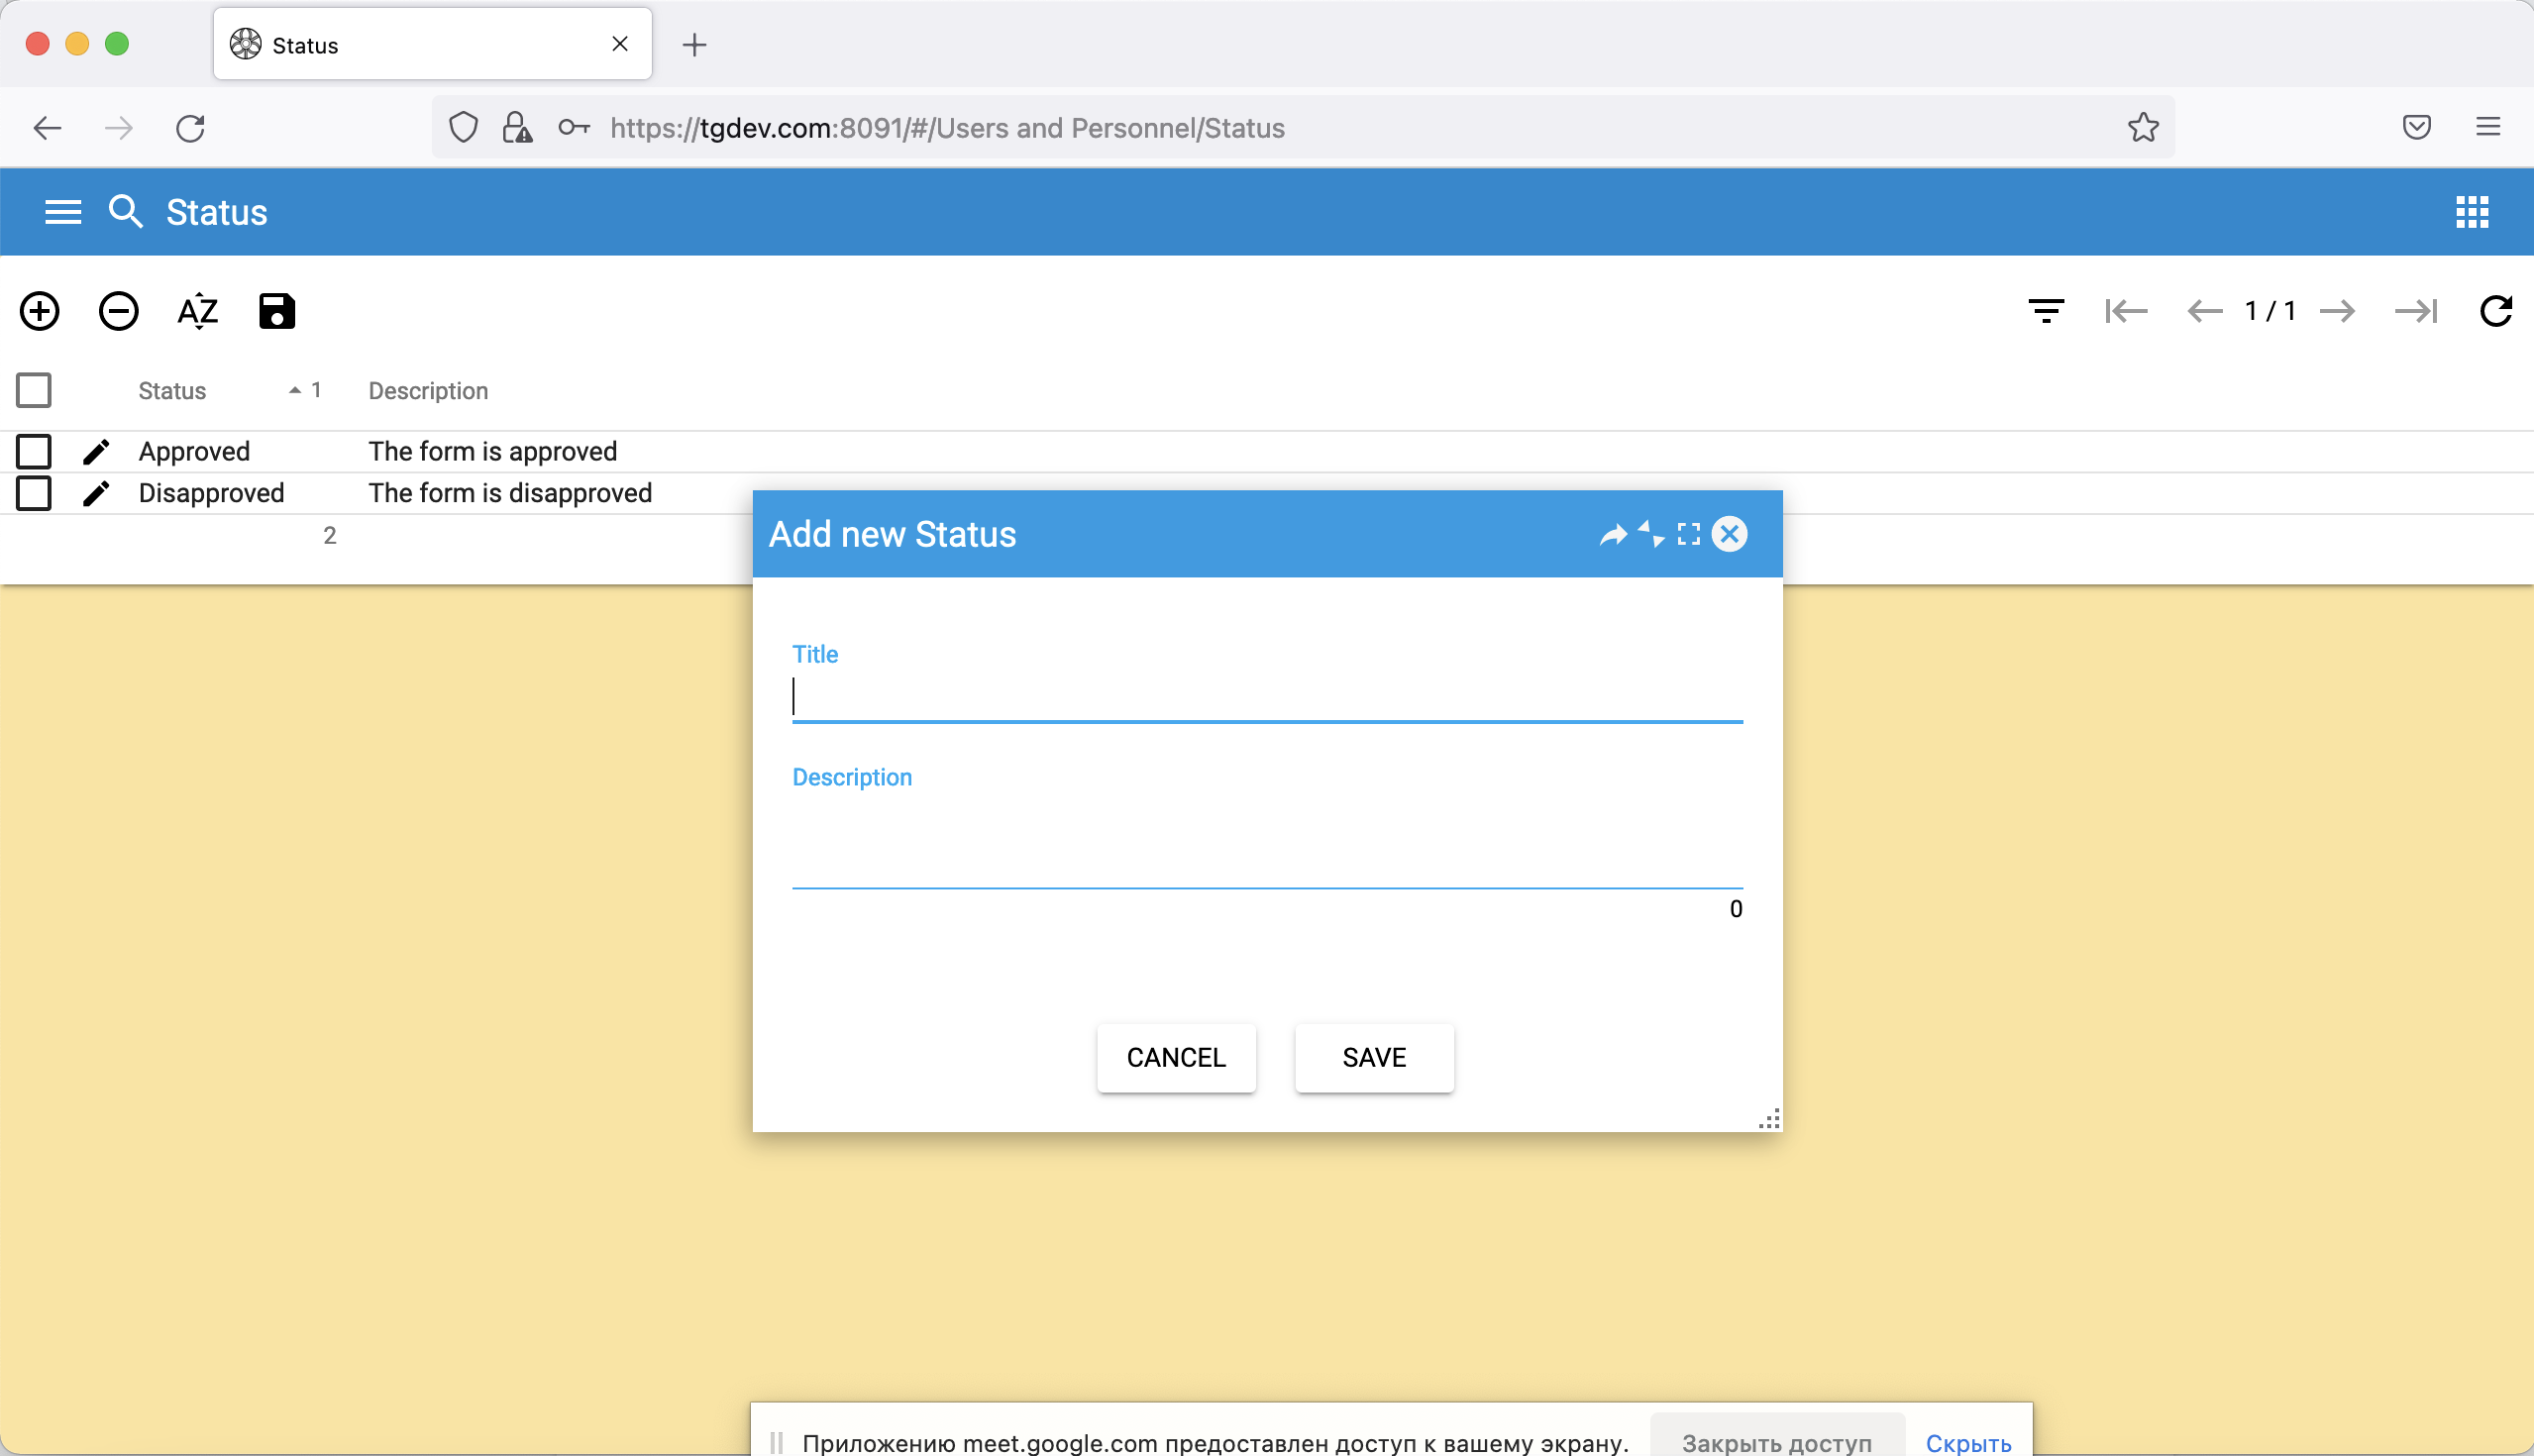
\includegraphics[width=0.95\linewidth]{sections/personnel/images/16.png}
\caption{Status creation.}\label{sections/personnel/images/16}
\end{figure}

\newpage
Users can also search for existing statuses either by specifying title, which is auto-completed, or description, or both, as displayed on
\hyperref[sections/personnel/images/17]{Fig.~\ref*{sections/personnel/images/17}}.

\begin{figure}[!htbp]
\centering
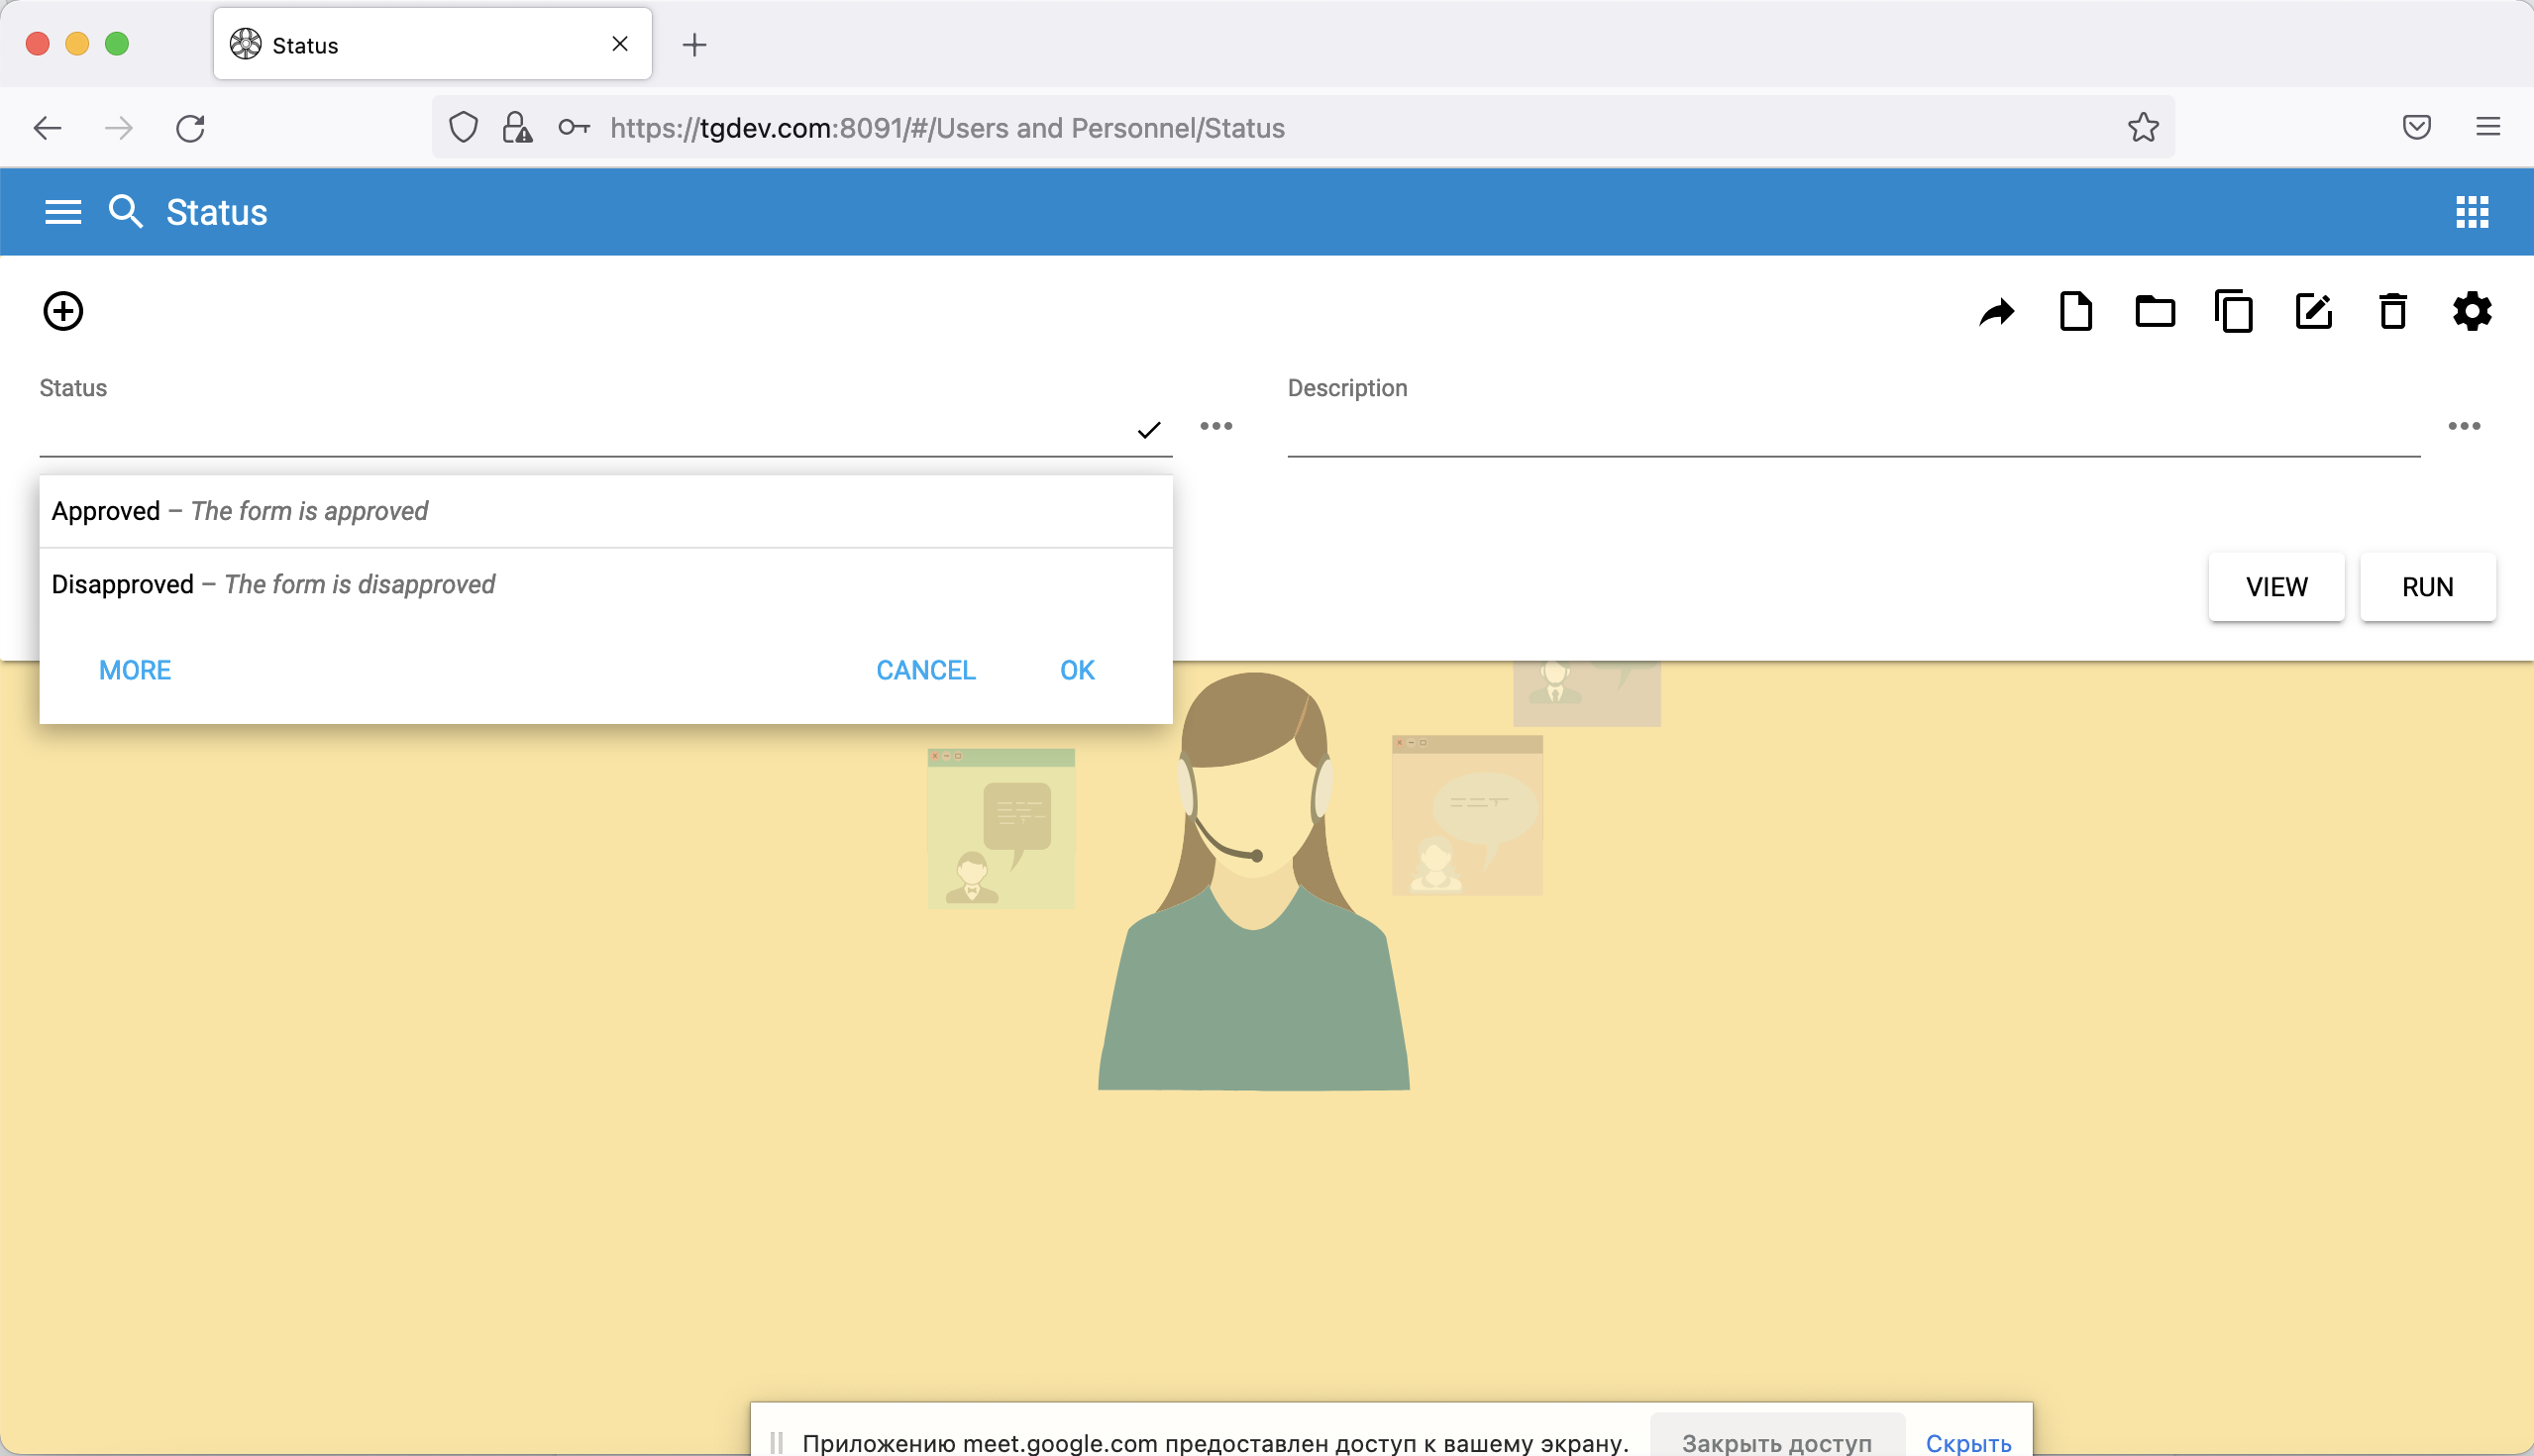
\includegraphics[width=0.95\linewidth]{sections/personnel/images/17.png}
\caption{Status search query.}\label{sections/personnel/images/17}
\end{figure}

\newpage
Search results are displayed along with title and description of the relevant statuses, as displayed on 
\hyperref[sections/personnel/images/18]{Fig.~\ref*{sections/personnel/images/18}}.

\begin{figure}[!htbp]
\centering
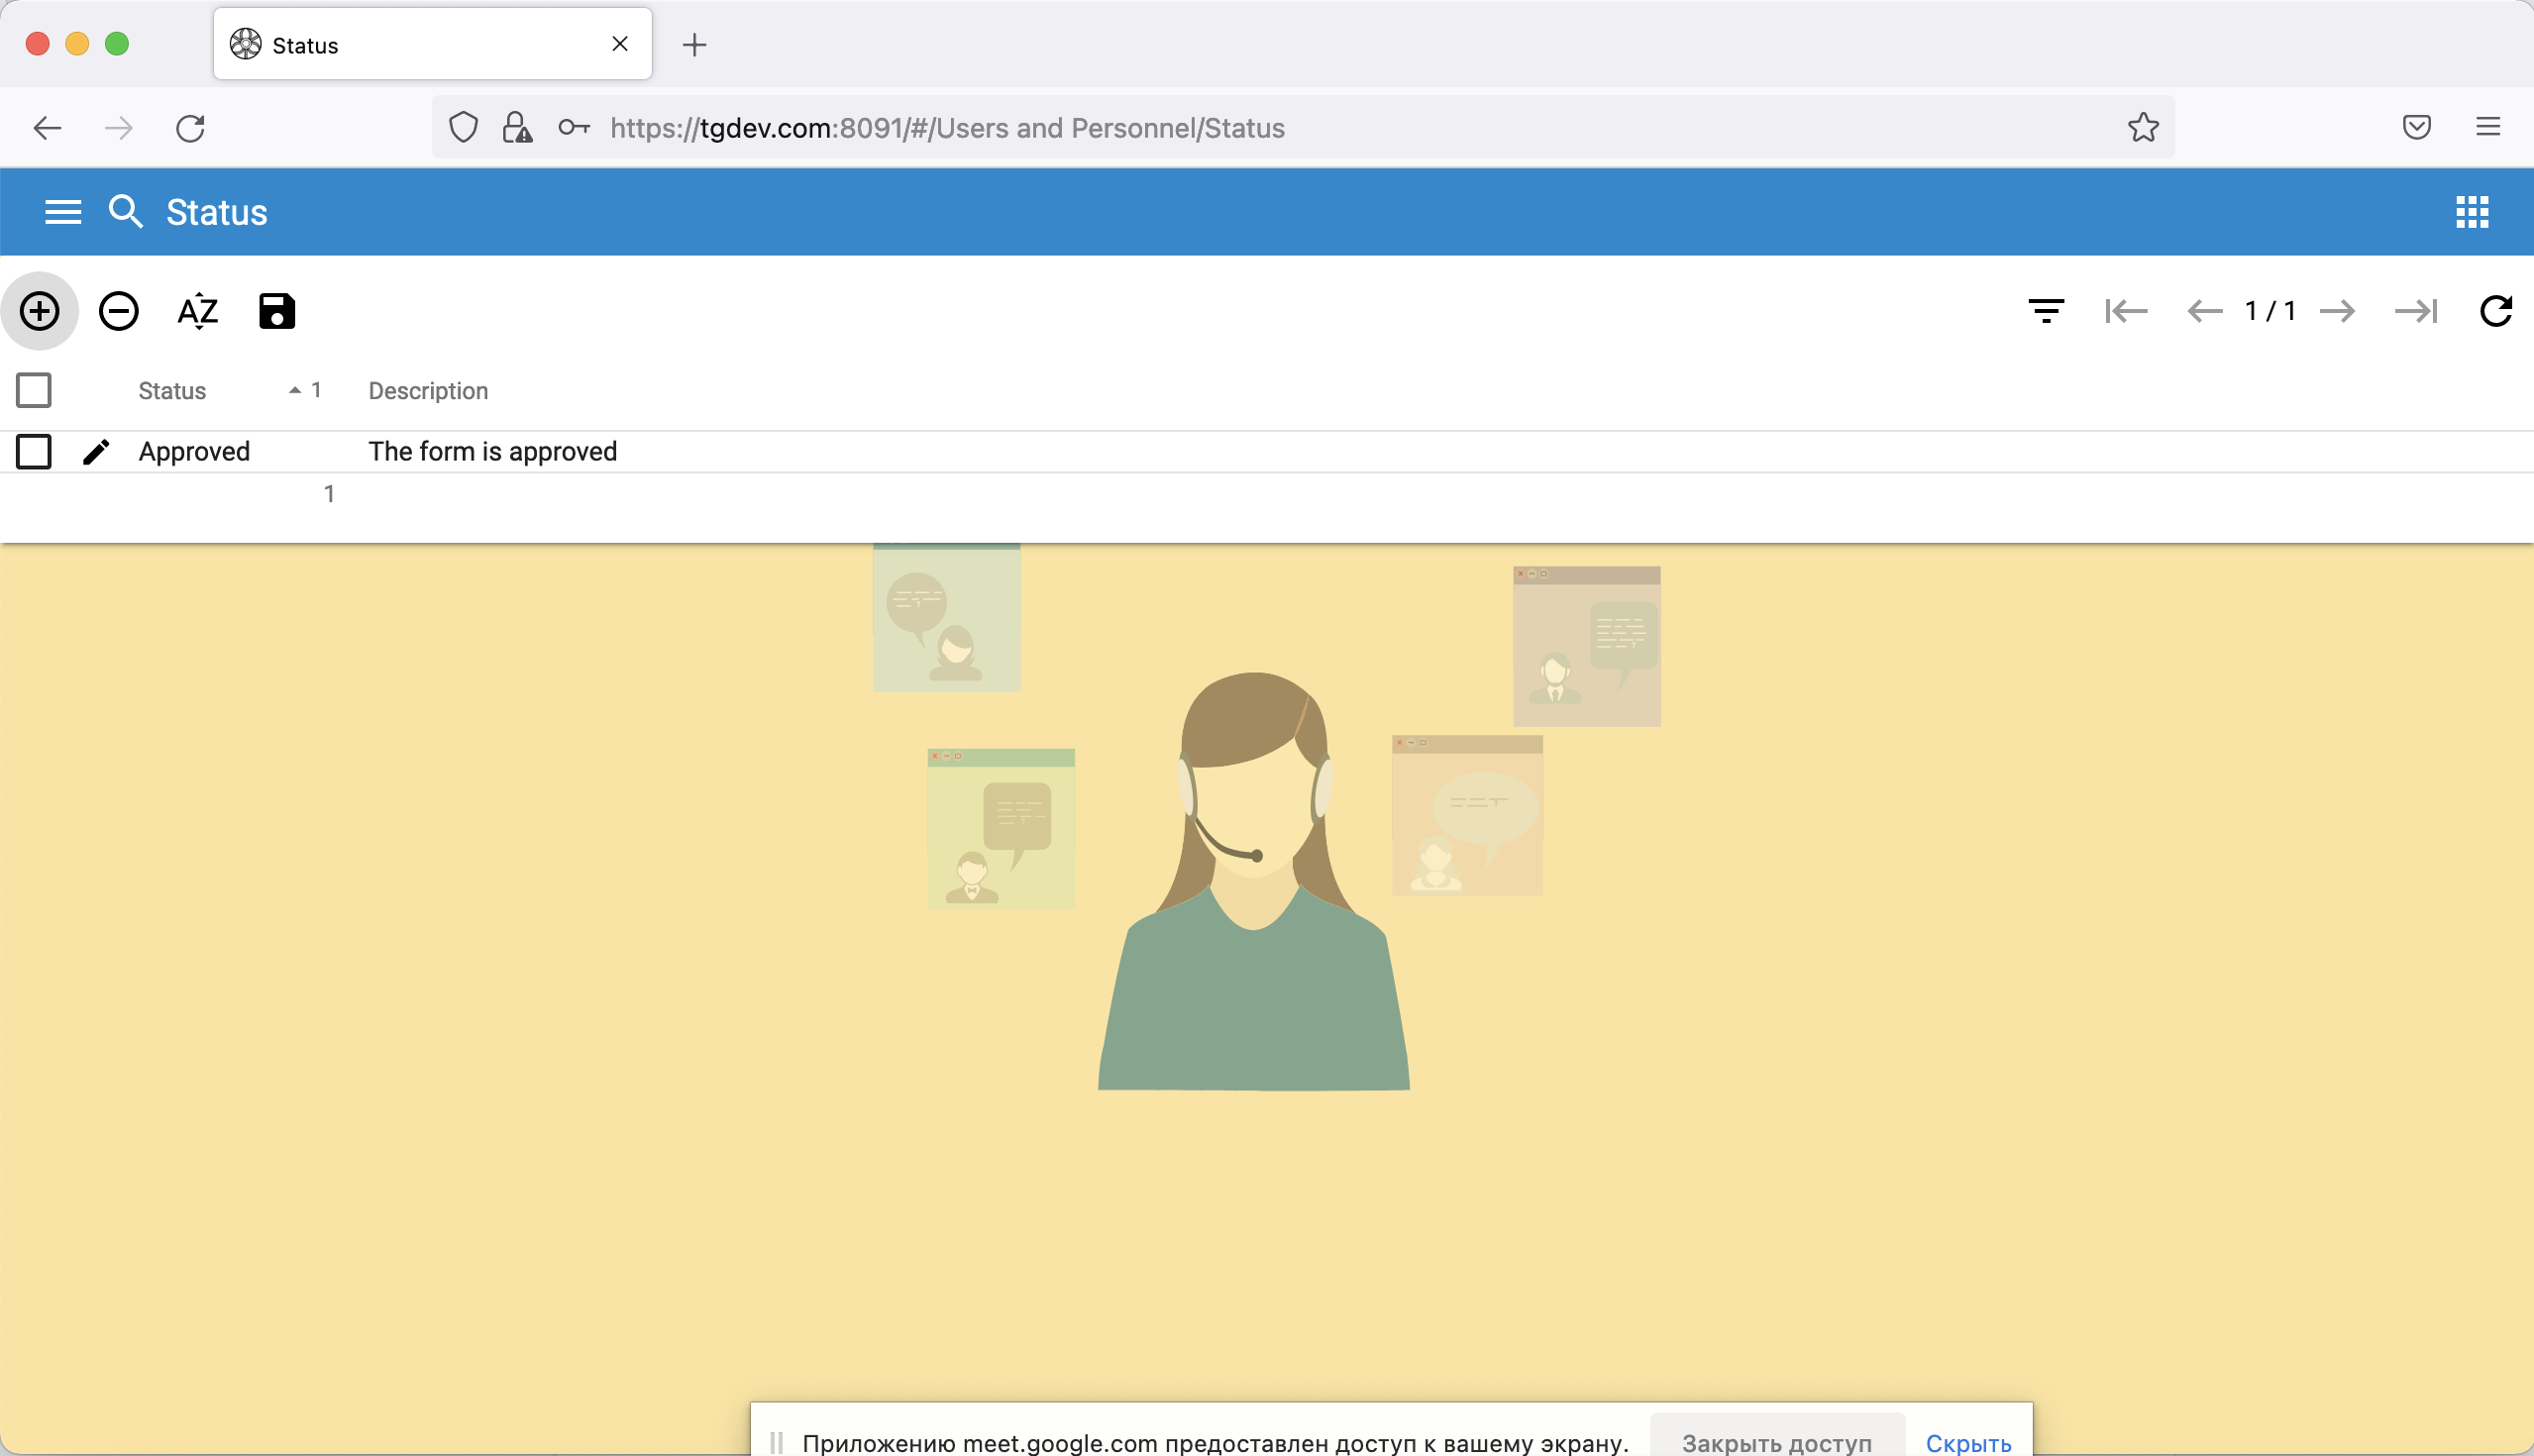
\includegraphics[width=0.95\linewidth]{sections/personnel/images/18.png}
\caption{Status search results.}\label{sections/personnel/images/18}
\end{figure}

\newpage
Users can edit existing statuses. As displayed on \hyperref[sections/personnel/images/19]{Fig.~\ref*{sections/personnel/images/19}}, users can edit title, and description of the specific status.

\begin{figure}[!htbp]
\centering
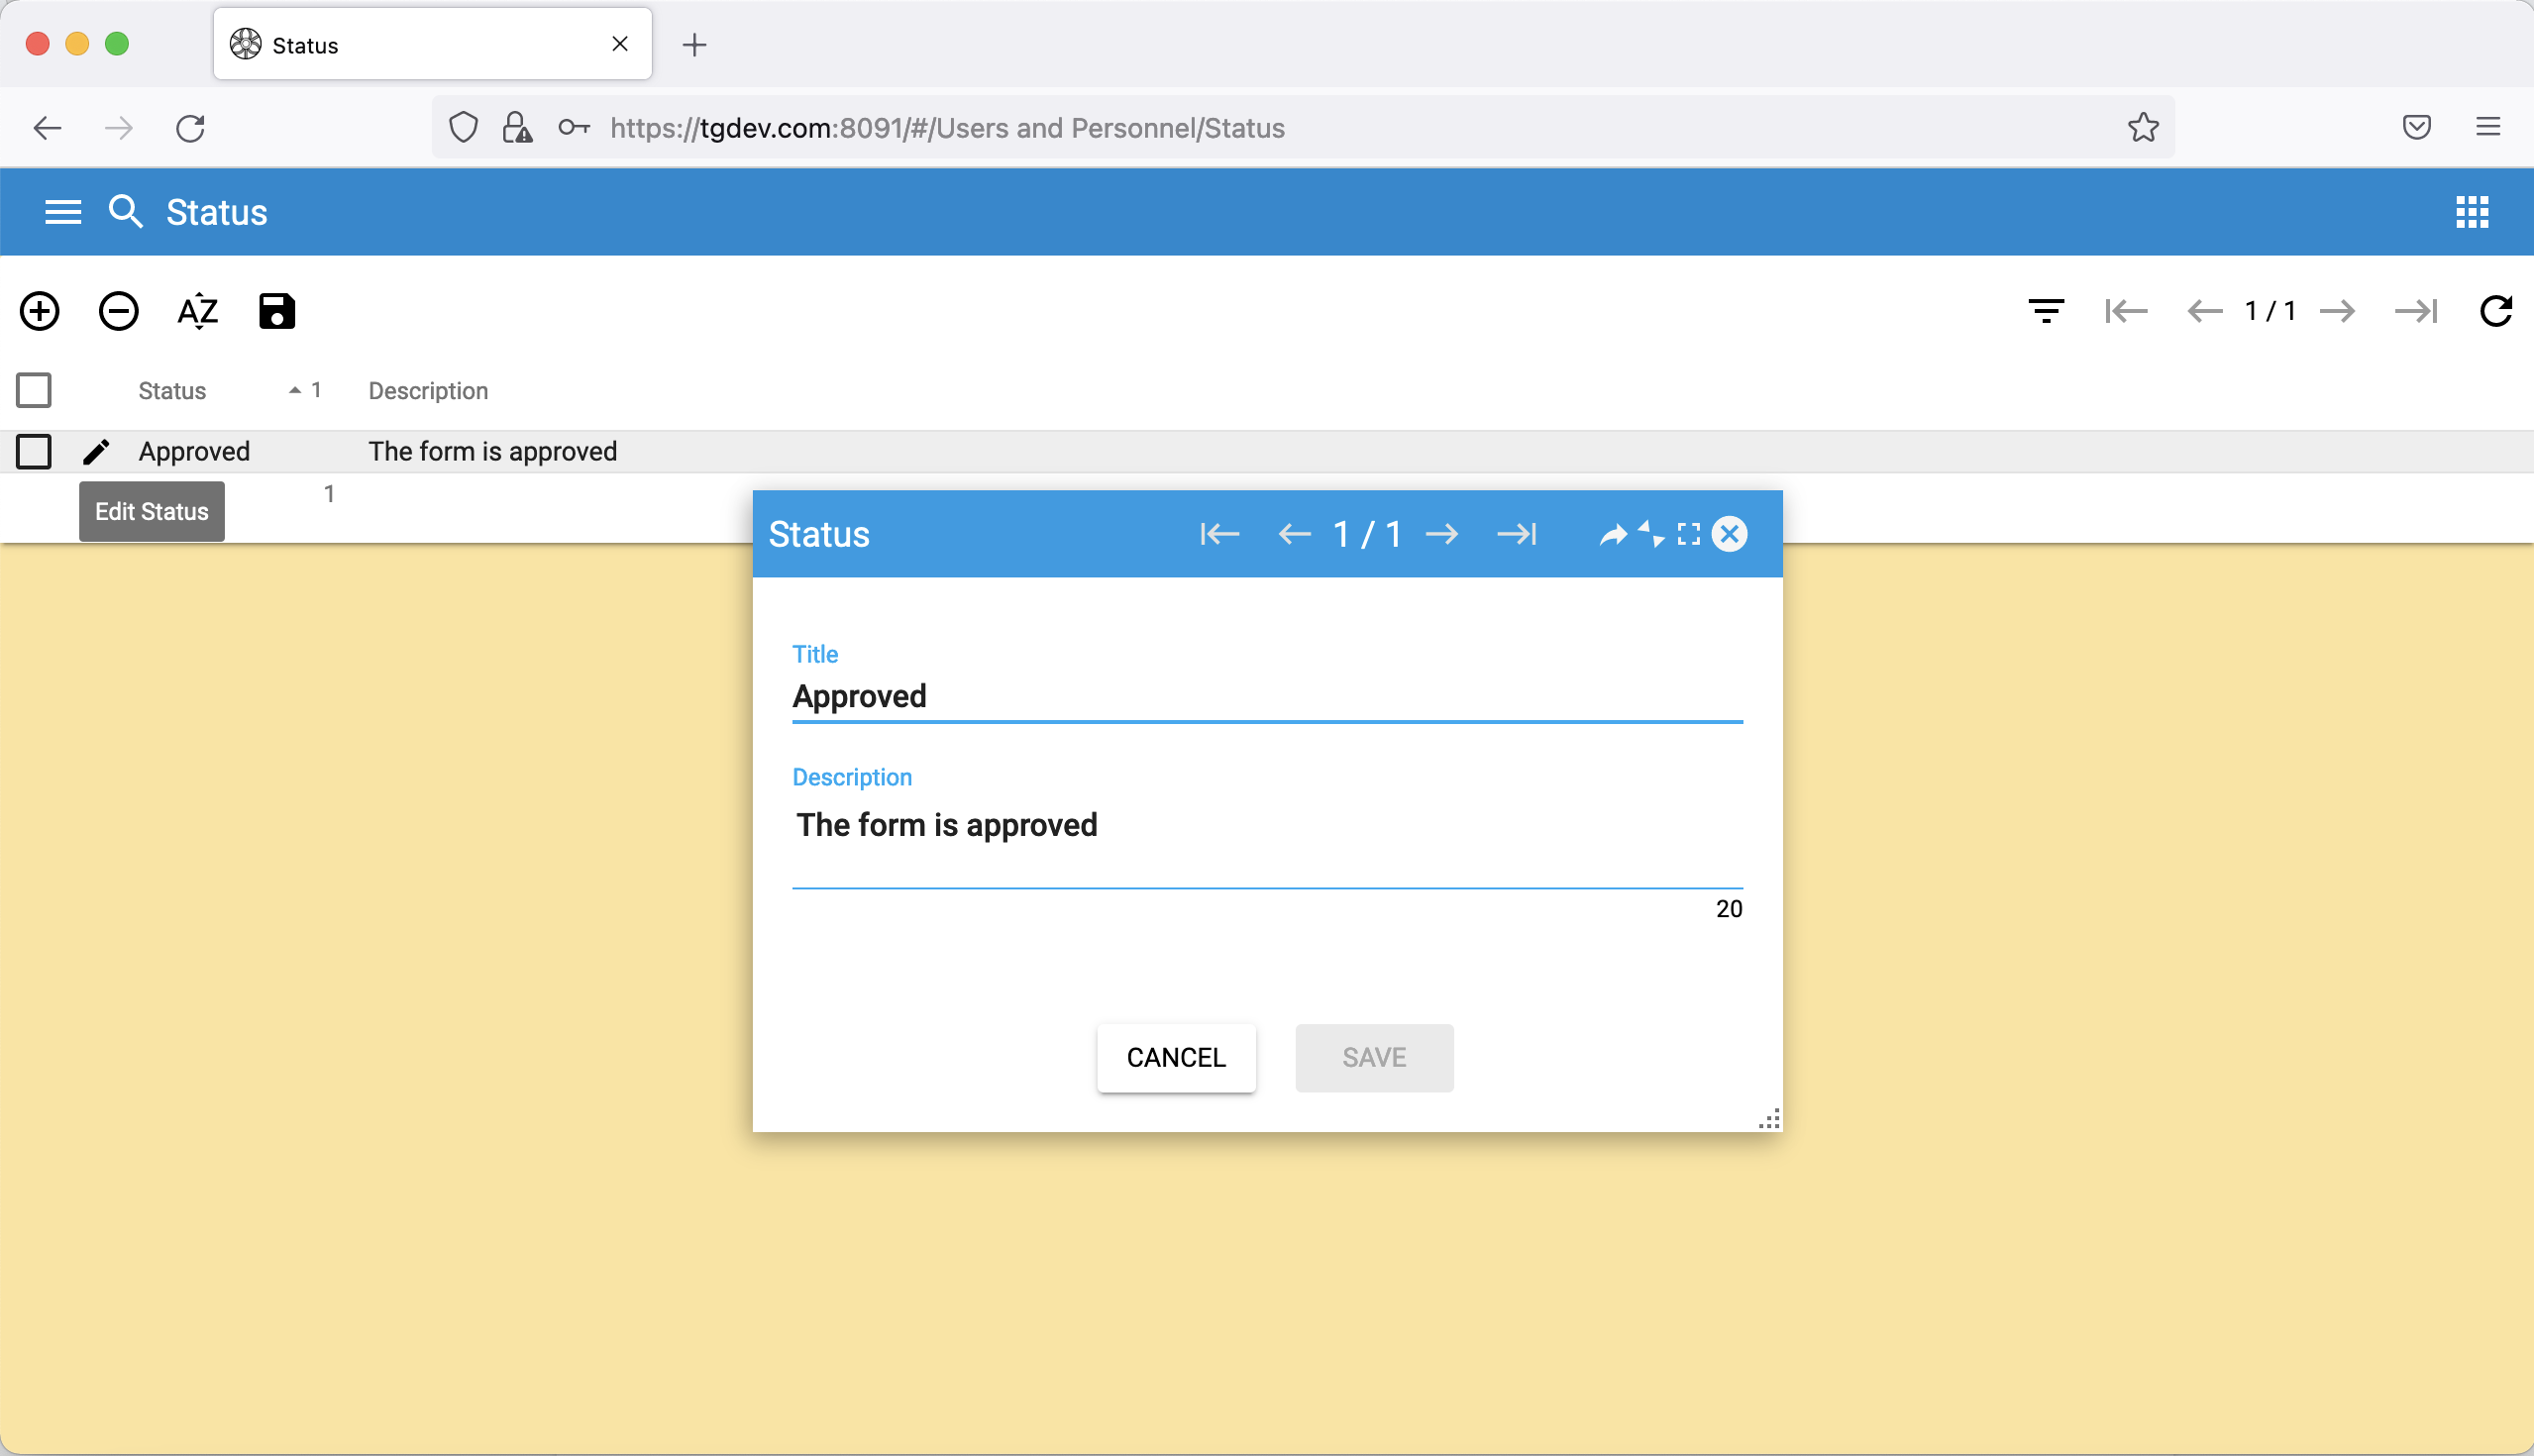
\includegraphics[width=0.95\linewidth]{sections/personnel/images/19.png}
\caption{Status editing.}\label{sections/personnel/images/19}
\end{figure}

\newpage
\subsection{Person}

In order to perform registration and save information about workers, users can create persons. When creating a new person, users have to fill in his/her name and surname, email, phone number in format +38 (098) 765 4321 (optional) and activity status, as displayed on \hyperref[sections/personnel/images/fig2]{Fig.~\ref*{sections/personnel/images/fig2}}.

\begin{figure}[!htbp]
\centering
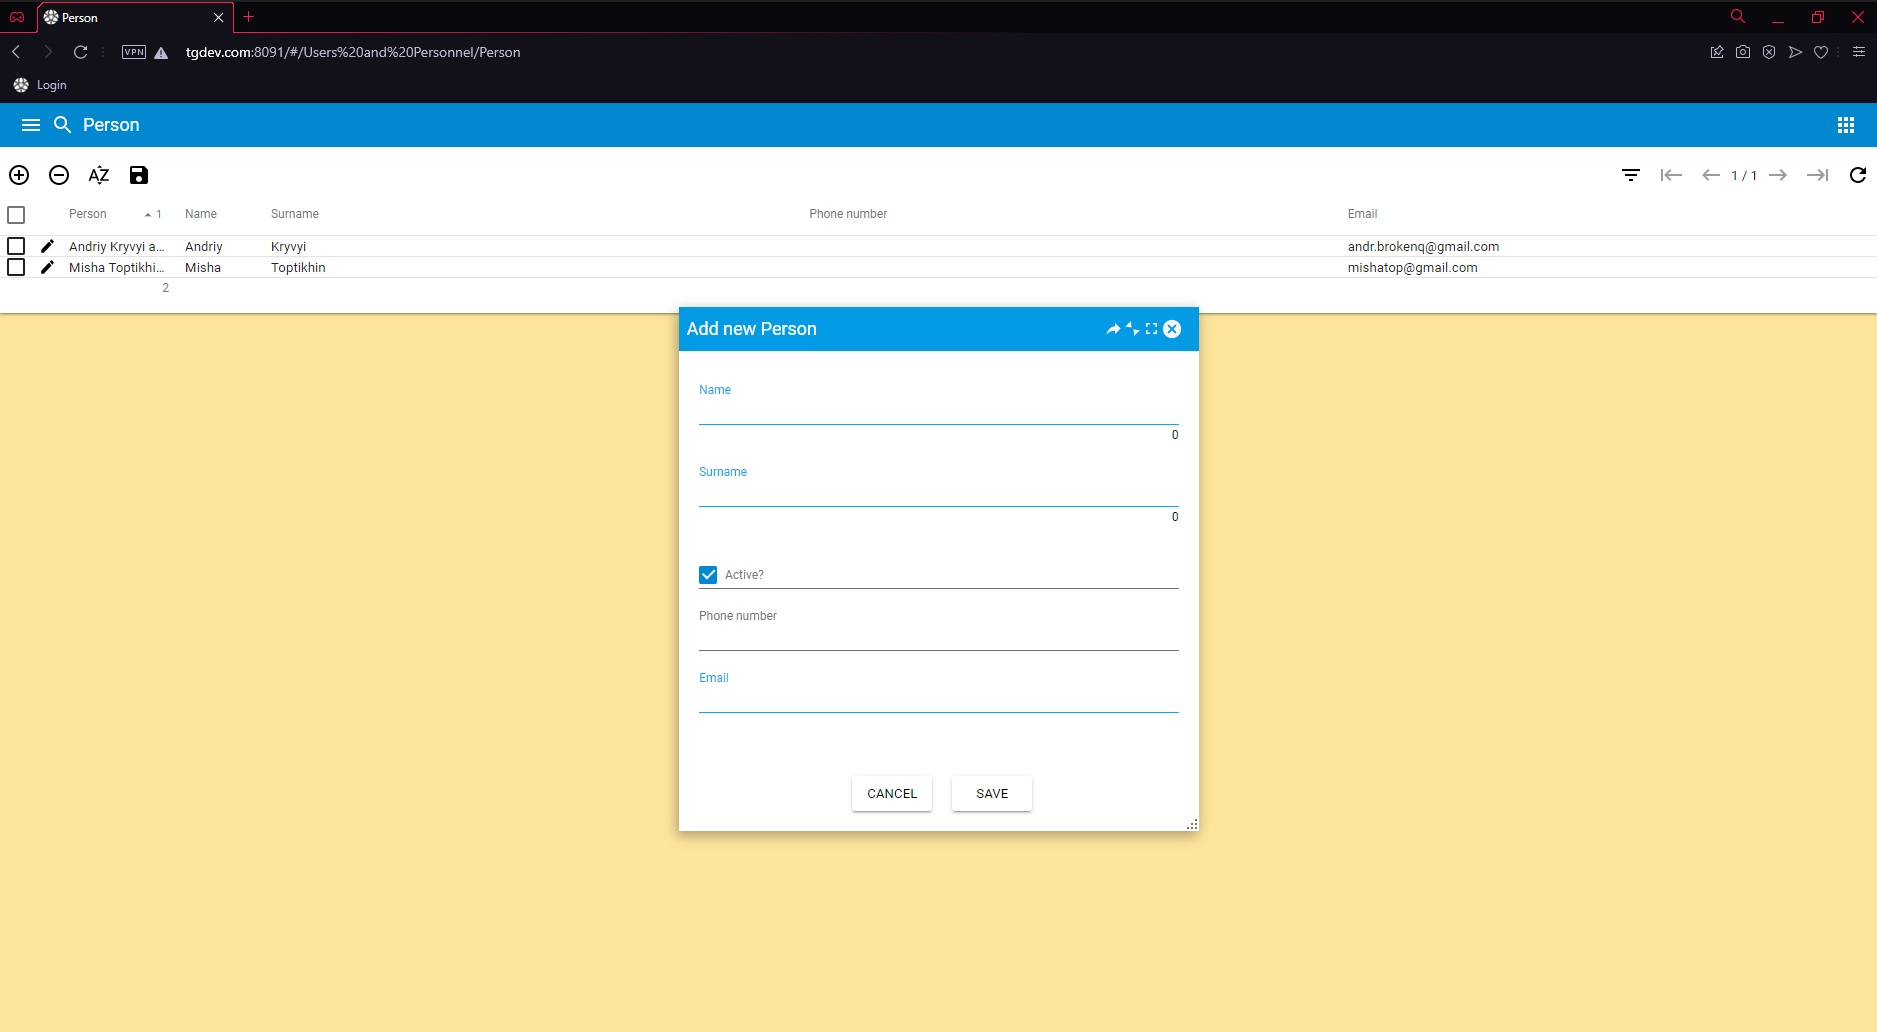
\includegraphics[width=0.95\linewidth]{sections/personnel/images/fig2.jpg}
\caption{Person creation.}\label{sections/personnel/images/fig2}
\end{figure}

\newpage
Users can search for existing persons either by specifying name, surname, or email, or phone number or activity status, or all of them as displayed on \hyperref[sections/personnel/images/fig1]{Fig.~\ref*{sections/personnel/images/fig1}}.

\begin{figure}[!htbp]
\centering
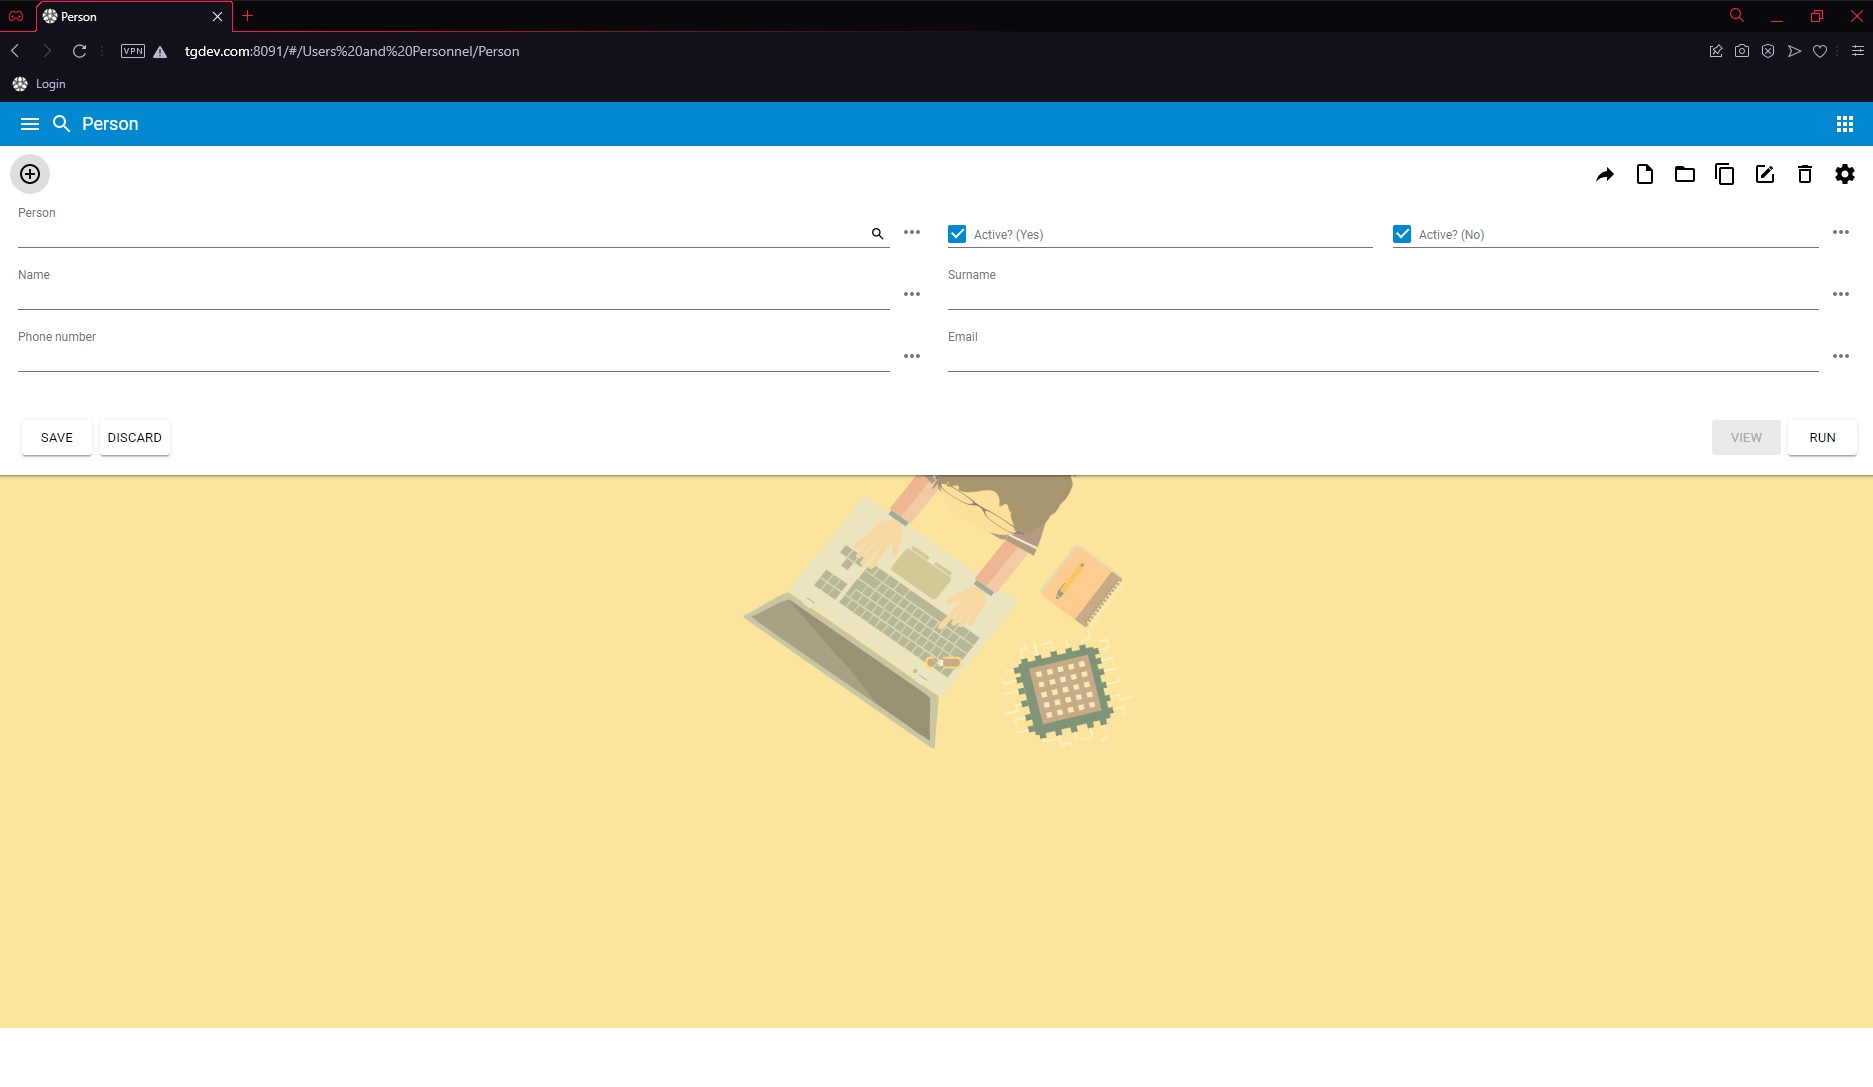
\includegraphics[width=0.95\linewidth]{sections/personnel/images/fig1.jpg}
\caption{Person search.}\label{sections/personnel/images/fig1}
\end{figure}

\newpage
Users can edit existing persons. On the ‘Main’ tab, displayed on \hyperref[sections/personnel/images/fig3]{Fig.~\ref*{sections/personnel/images/fig3}}, users can edit the name, surname, phone number, email and activity status of the specific person.

\begin{figure}[!htbp]
\centering
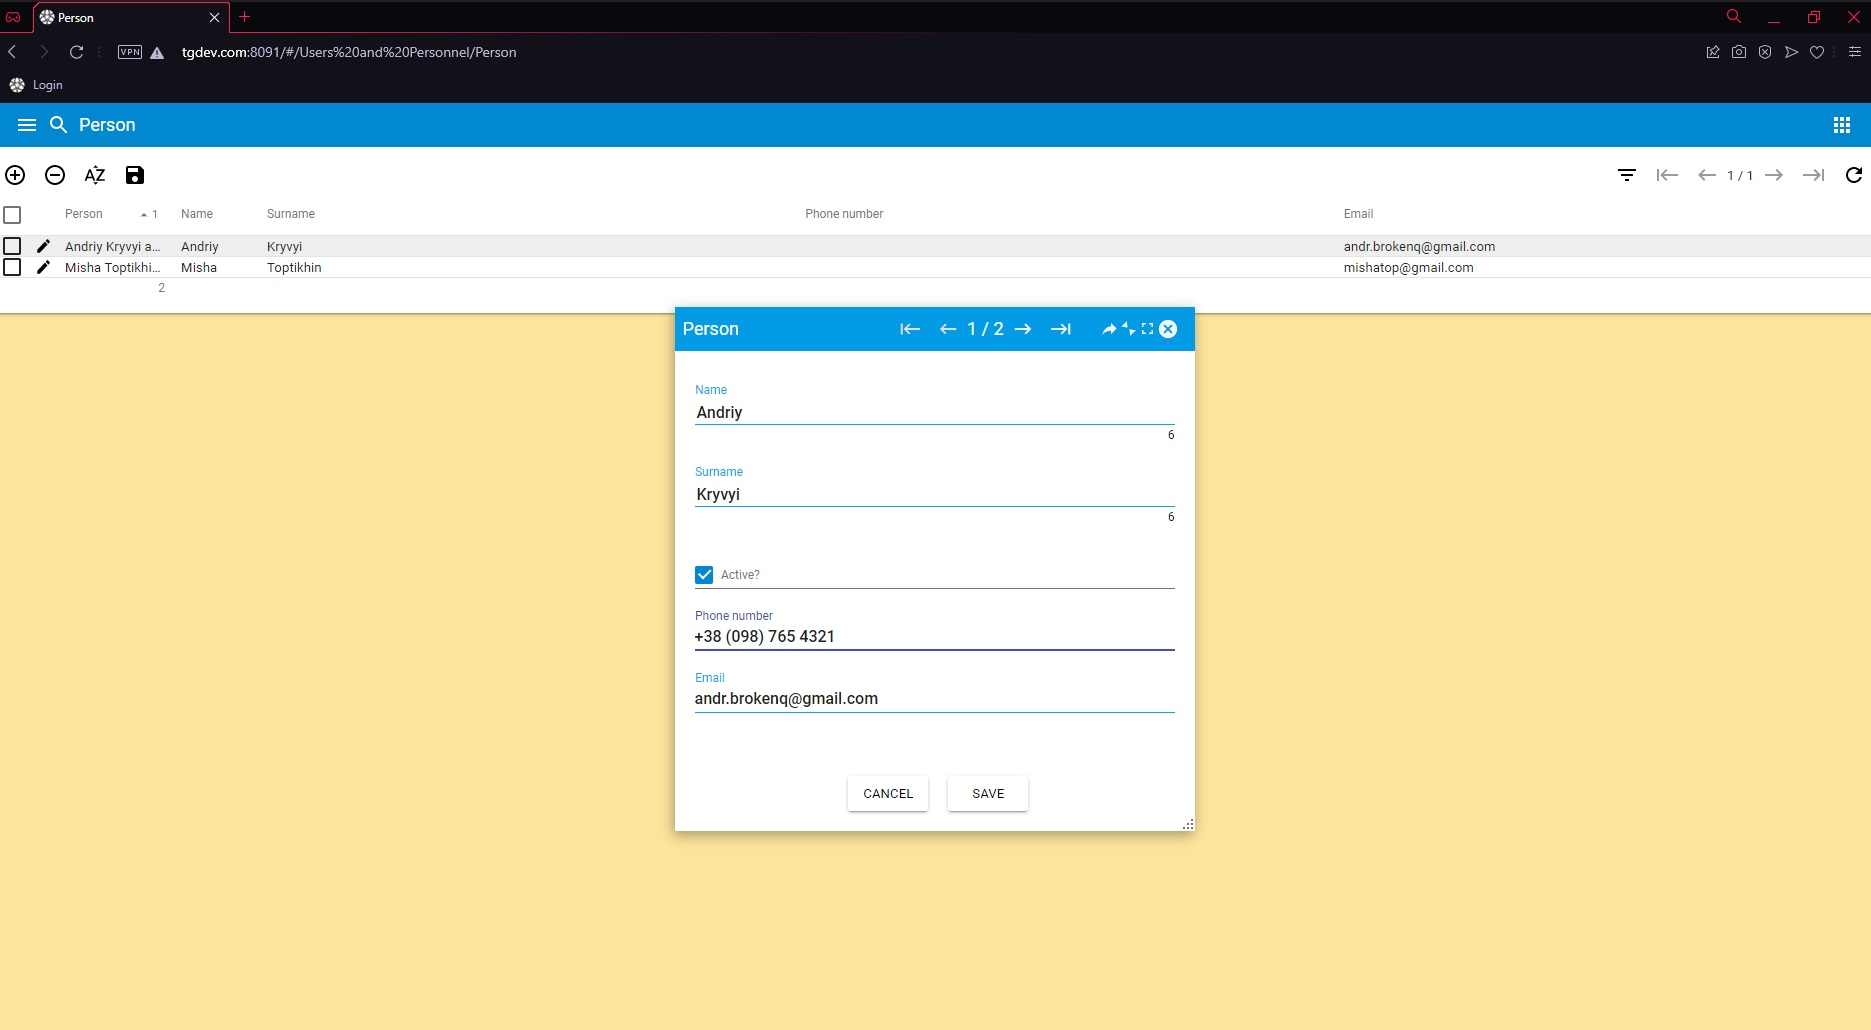
\includegraphics[width=0.95\linewidth]{sections/personnel/images/fig3.jpg}
\caption{Person editing.}\label{sections/personnel/images/fig3}
\end{figure}

\newpage
\subsection{Role}

In order to create and save roles, which will help to record the responsibility of workers, users can create roles. When creating a new role, users have to fill in its title and description as displayed on
\hyperref[sections/personnel/images/fig5]{Fig.~\ref*{sections/personnel/images/fig5}}.

\begin{figure}[!htbp]
\centering
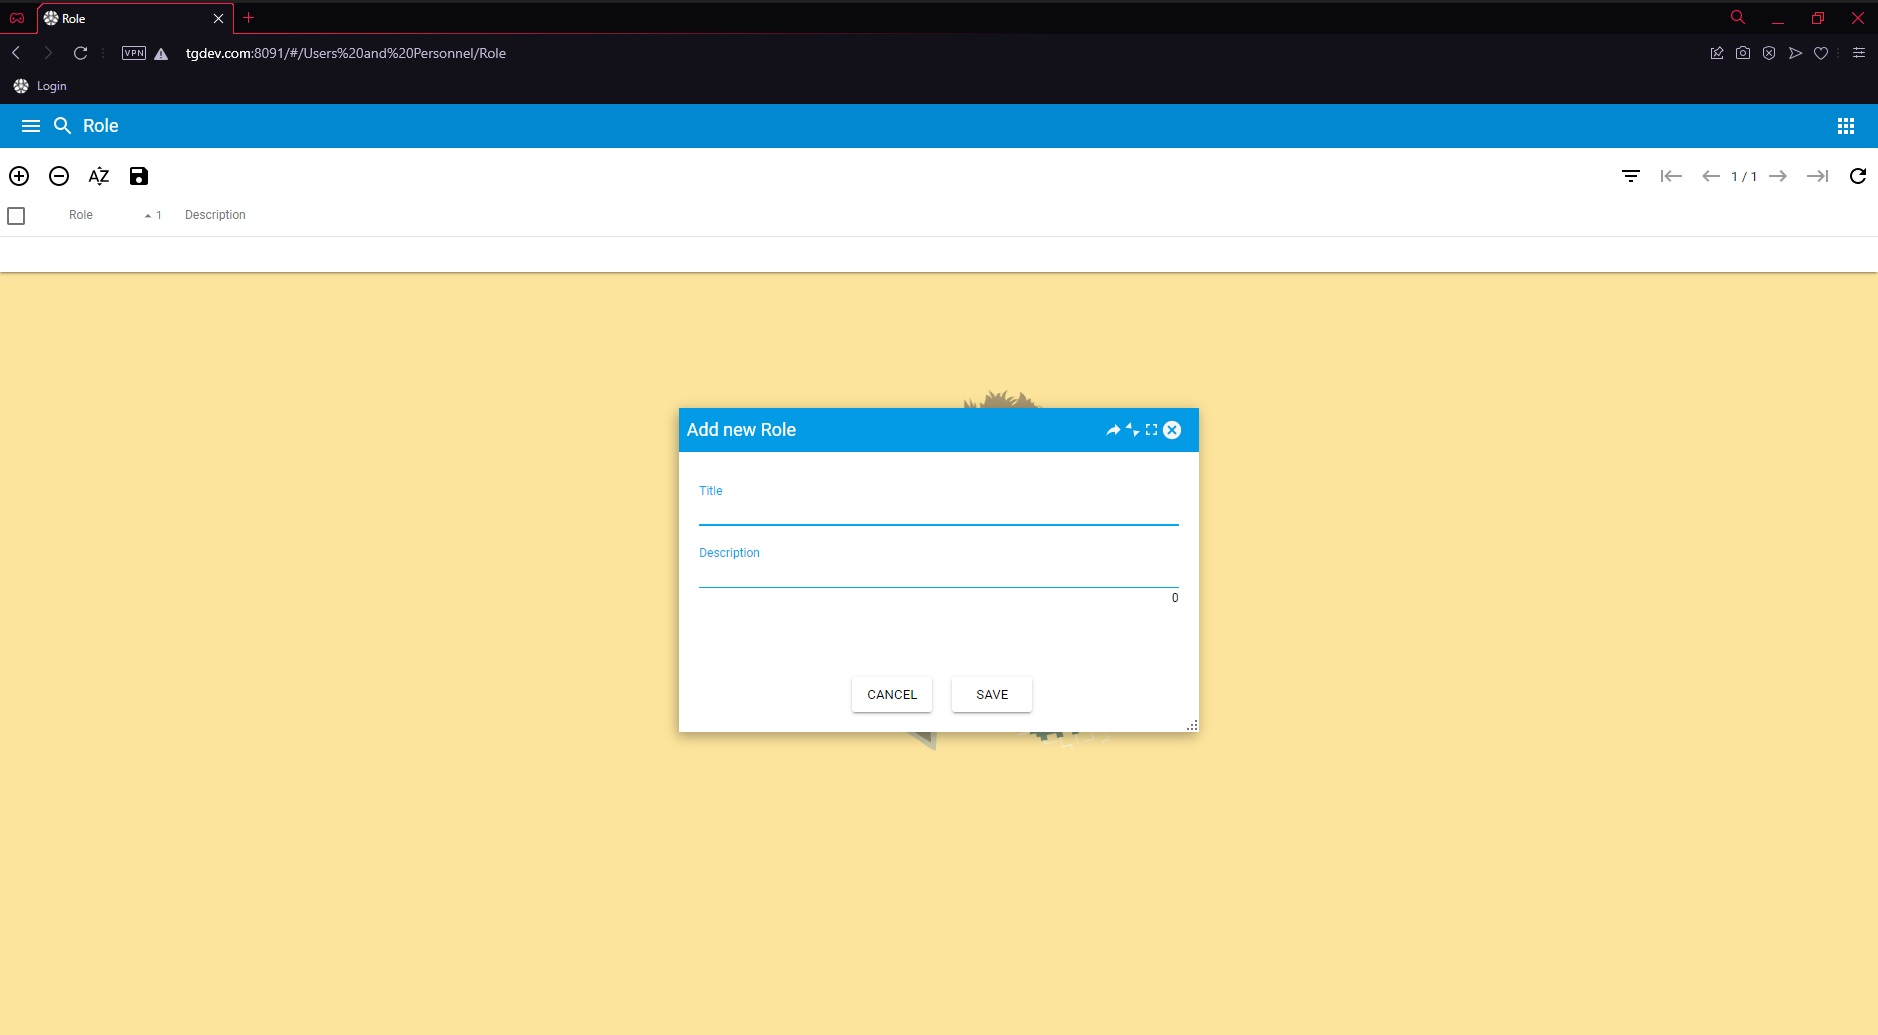
\includegraphics[width=0.95\linewidth]{sections/personnel/images/fig5.jpg}
\caption{Role creation.}\label{sections/personnel/images/fig5}
\end{figure}

\newpage
Users can search for existing roles either by specifying title, or description, or both as displayed on \hyperref[sections/personnel/images/fig4]{Fig.~\ref*{sections/personnel/images/fig4}}.

\begin{figure}[!htbp]
\centering
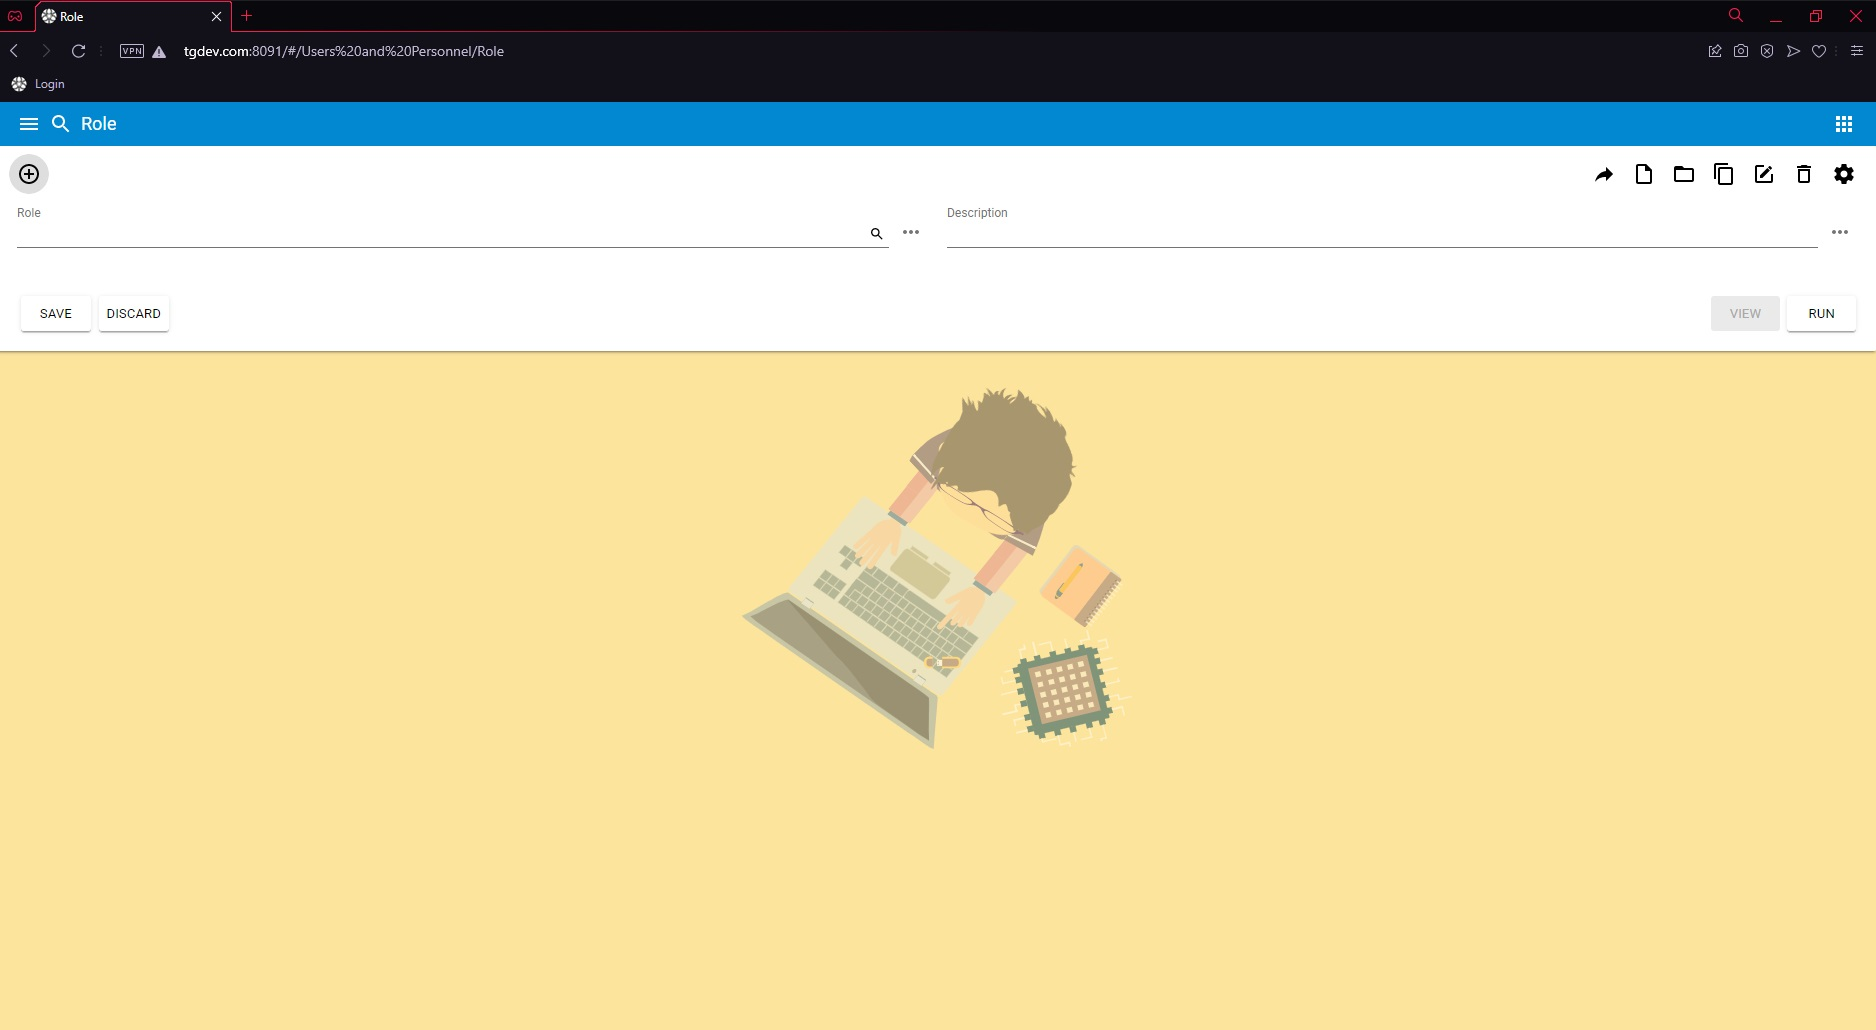
\includegraphics[width=0.95\linewidth]{sections/personnel/images/fig4.jpg}
\caption{Role search.}\label{sections/personnel/images/fig4}
\end{figure}

\newpage
Users can edit existing roles. On the ‘Main’ tab, displayed on \hyperref[sections/personnel/images/fig9]{Fig.~\ref*{sections/personnel/images/fig9}}, users can edit the title and description of the specific role.

\begin{figure}[!htbp]
\centering
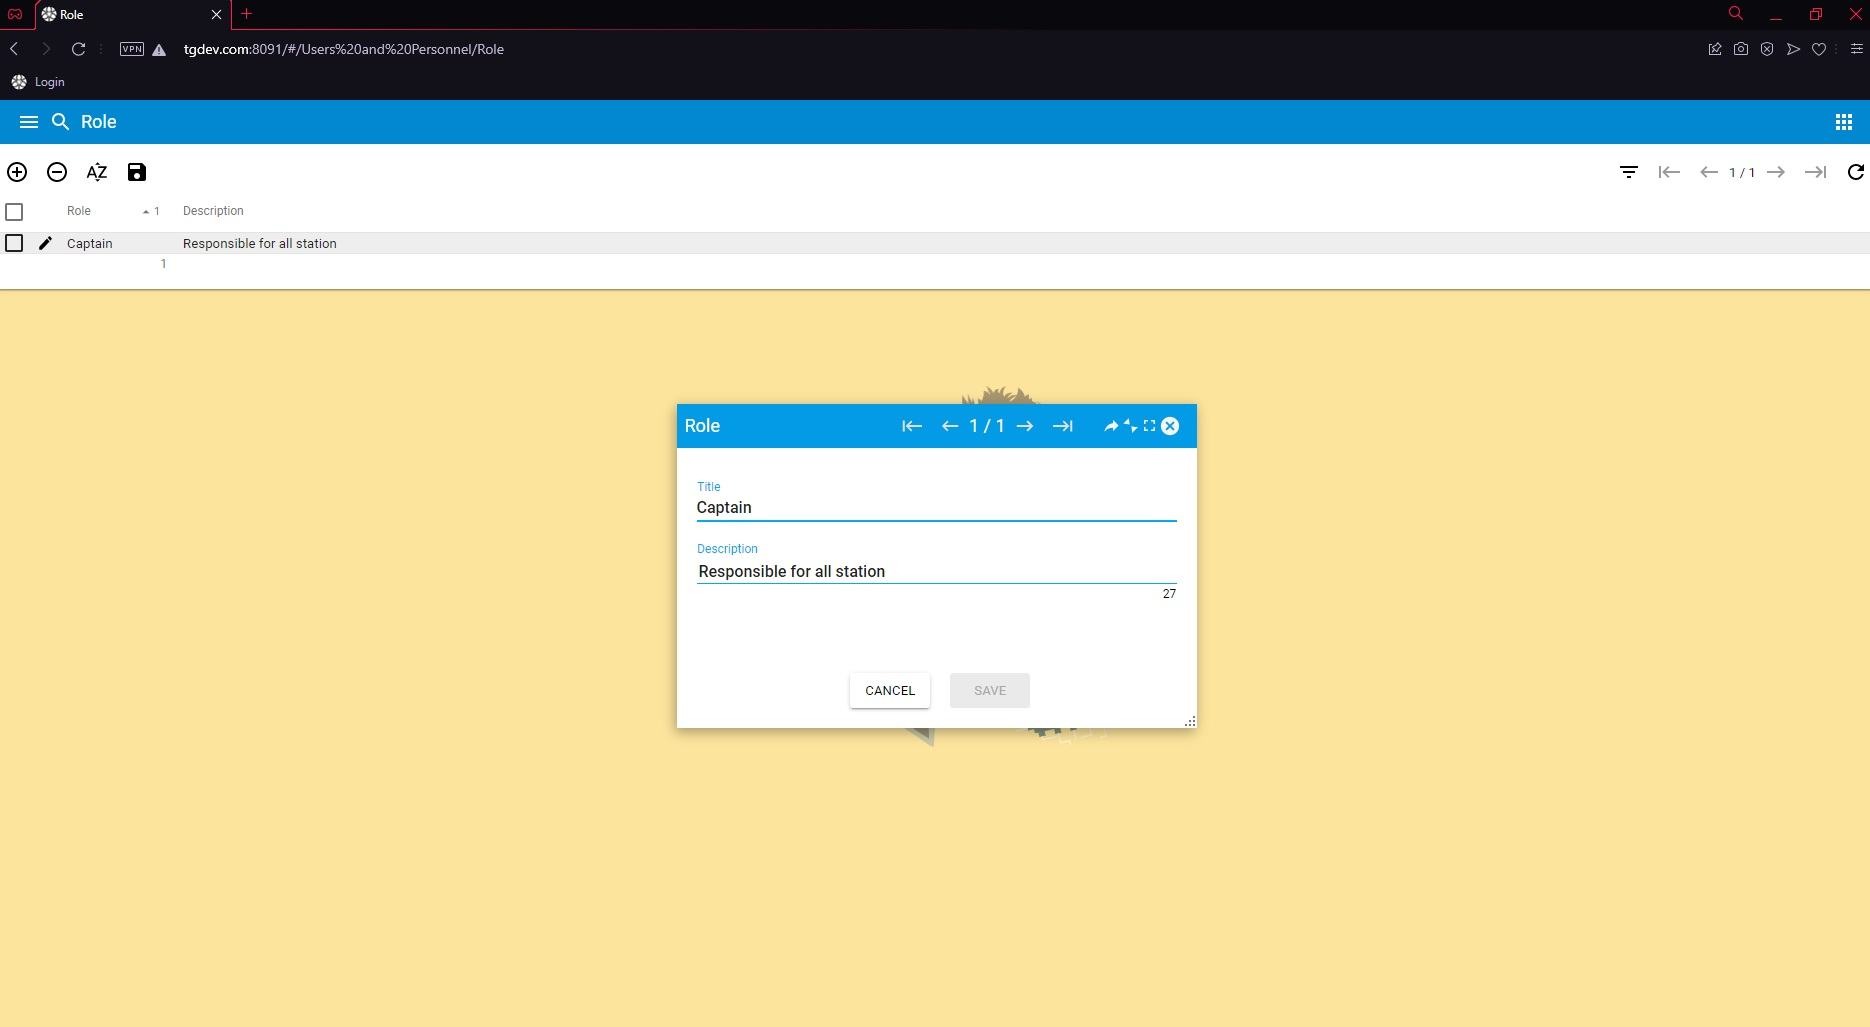
\includegraphics[width=0.95\linewidth]{sections/personnel/images/fig9.jpg}
\caption{Role editing.}\label{sections/personnel/images/fig9}
\end{figure}

\newpage
\subsection{Person role}

In order to assign a specific role to a worker at a specific date, users can create person role. When creating a new person role, users have to fill in the person, which is an autocomplete, role, which is also an autocomplete, and date when the role was assigned, as displayed on
\hyperref[sections/personnel/images/fig7]{Fig.~\ref*{sections/personnel/images/fig7}}.

\begin{figure}[!htbp]
\centering
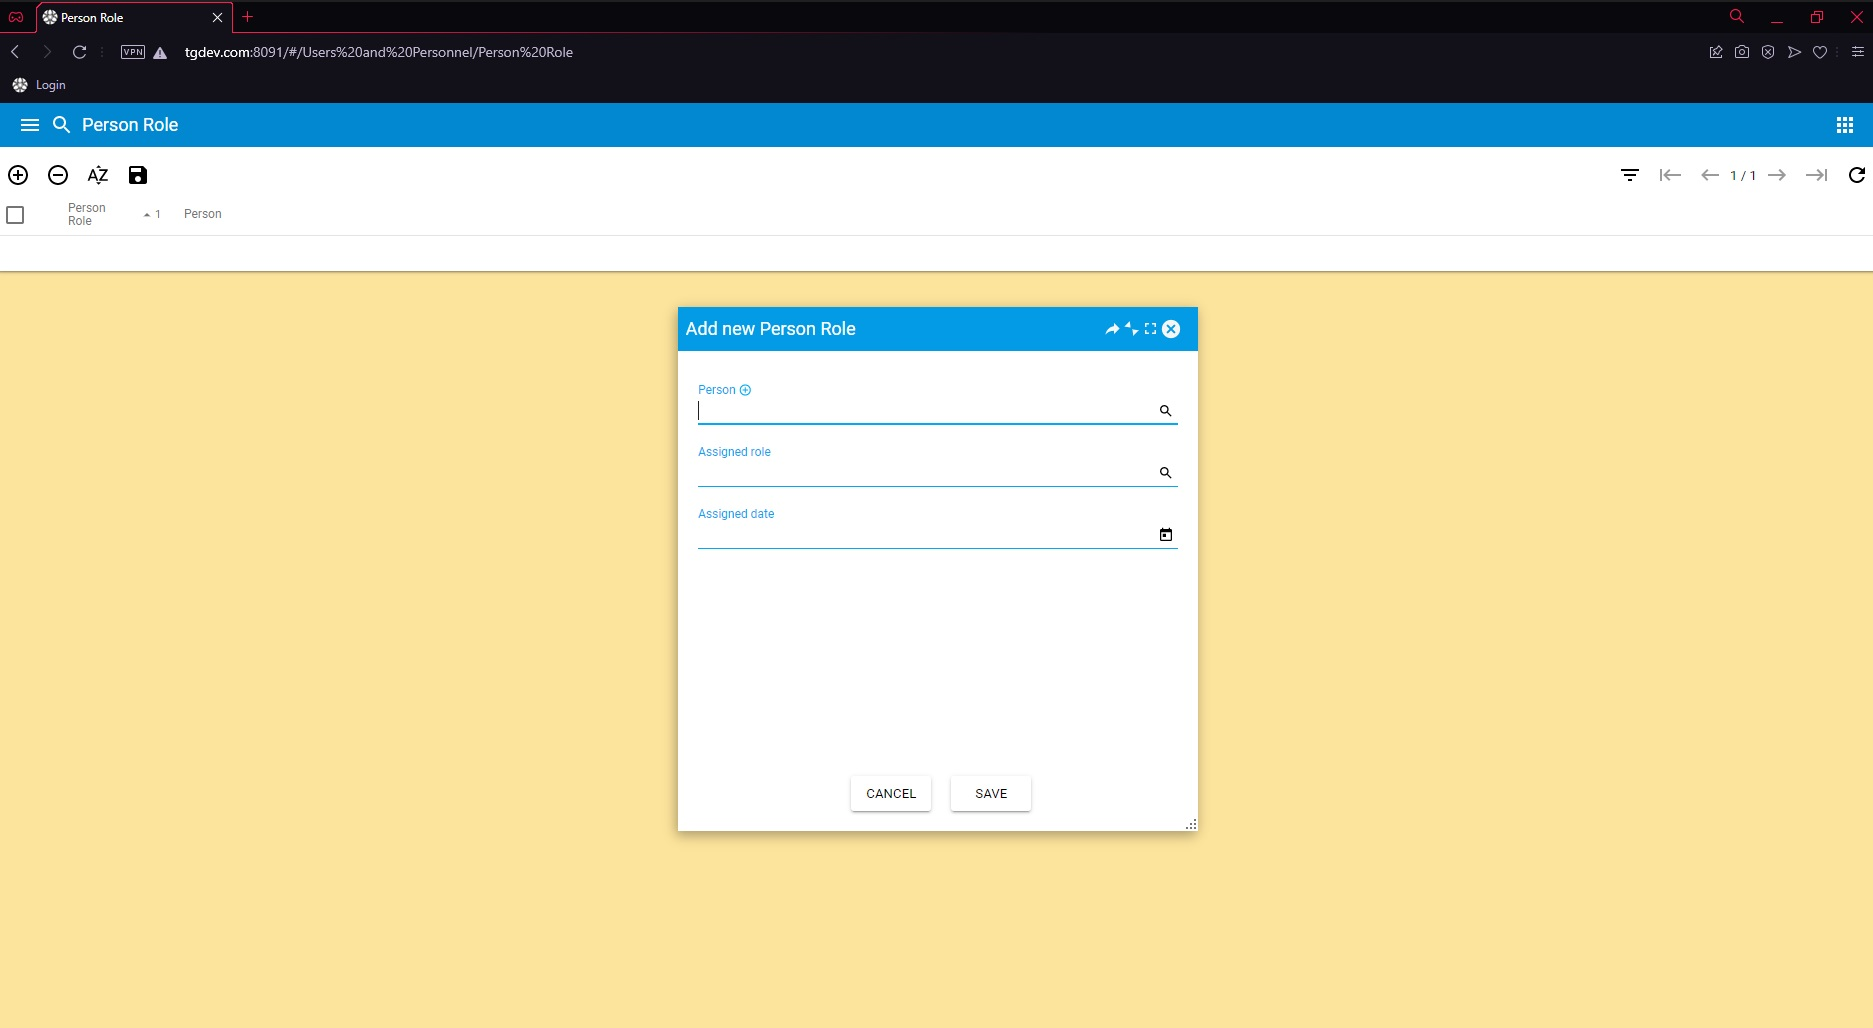
\includegraphics[width=0.95\linewidth]{sections/personnel/images/fig7.jpg}
\caption{Person role creation.}\label{sections/personnel/images/fig7}
\end{figure}

\newpage
Person and role fields have autocompletion so there is no need to type full person or role name by hand.

\begin{figure}[!htbp]
\centering
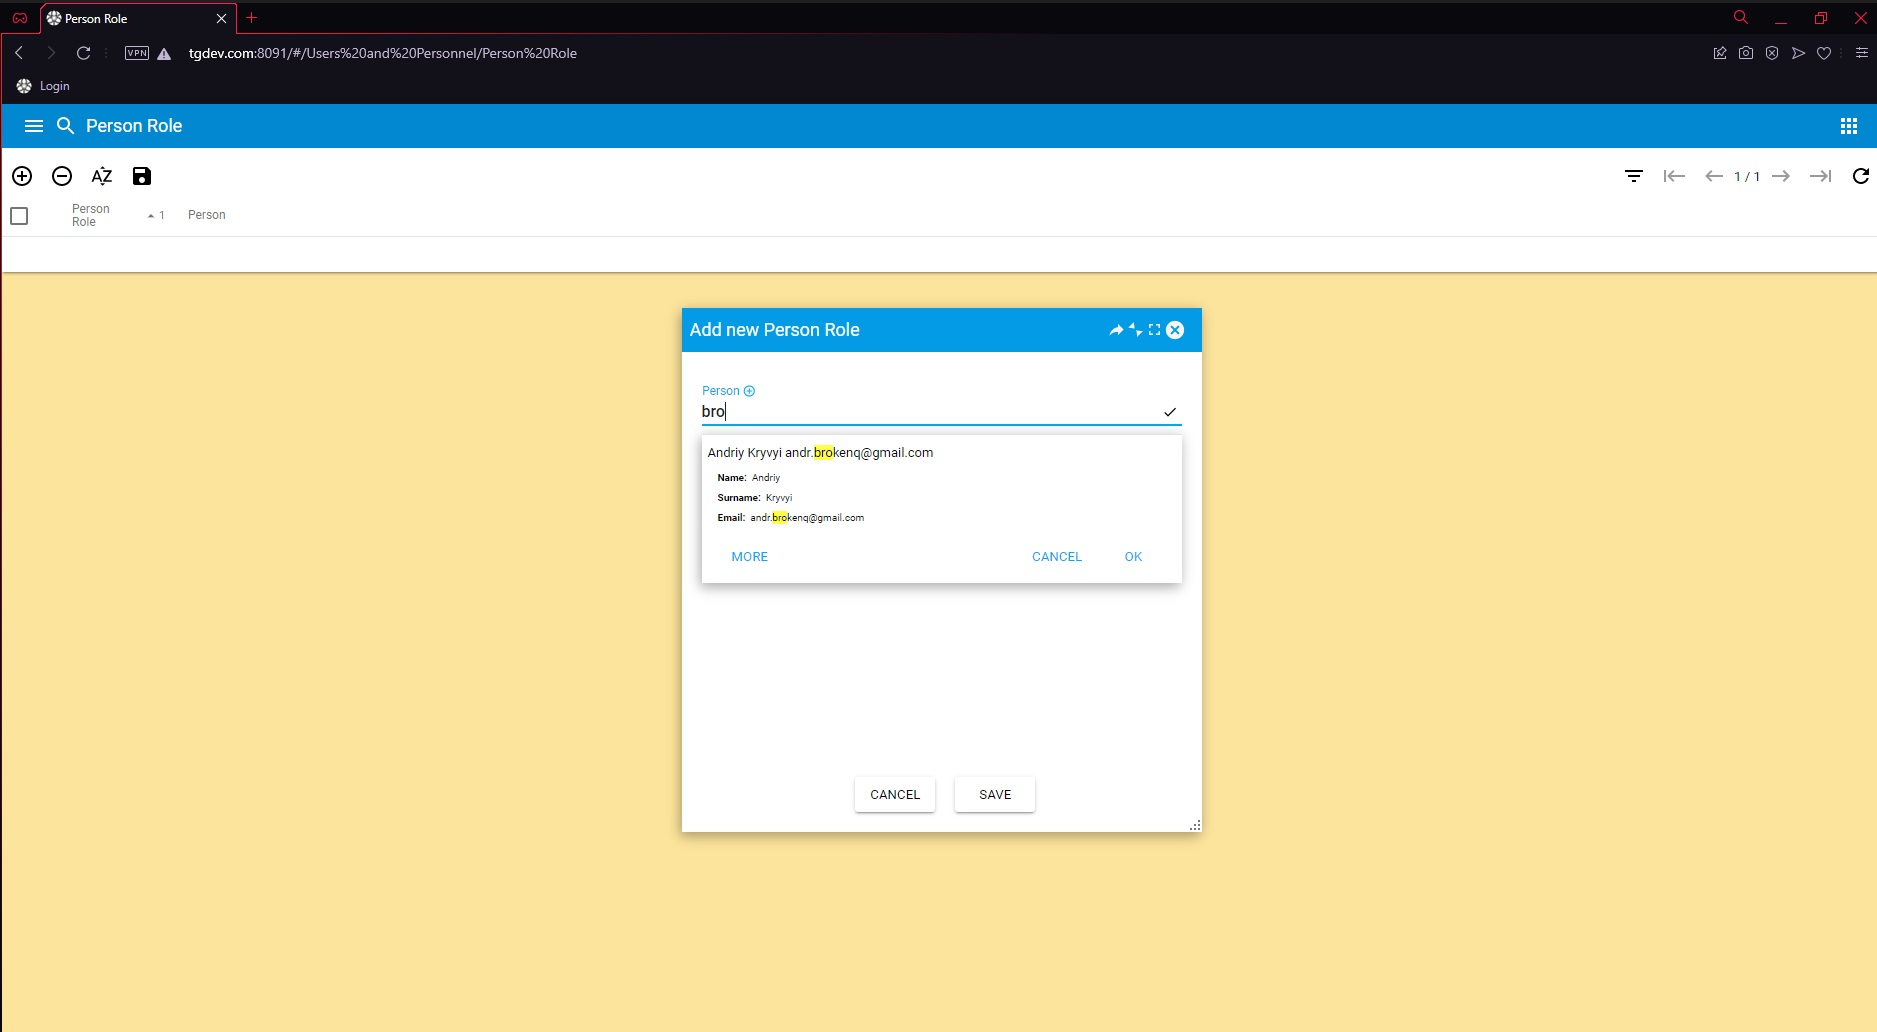
\includegraphics[width=0.95\linewidth]{sections/personnel/images/fig8.jpg}
\caption{Person field autocompletion.}\label{sections/personnel/images/fig8}
\end{figure}

\newpage
Users can search for existing person roles either by specifying person, or role, or date range, or all of them as displayed on \hyperref[sections/personnel/images/fig6]{Fig.~\ref*{sections/personnel/images/fig6}}.

\begin{figure}[!htbp]
\centering
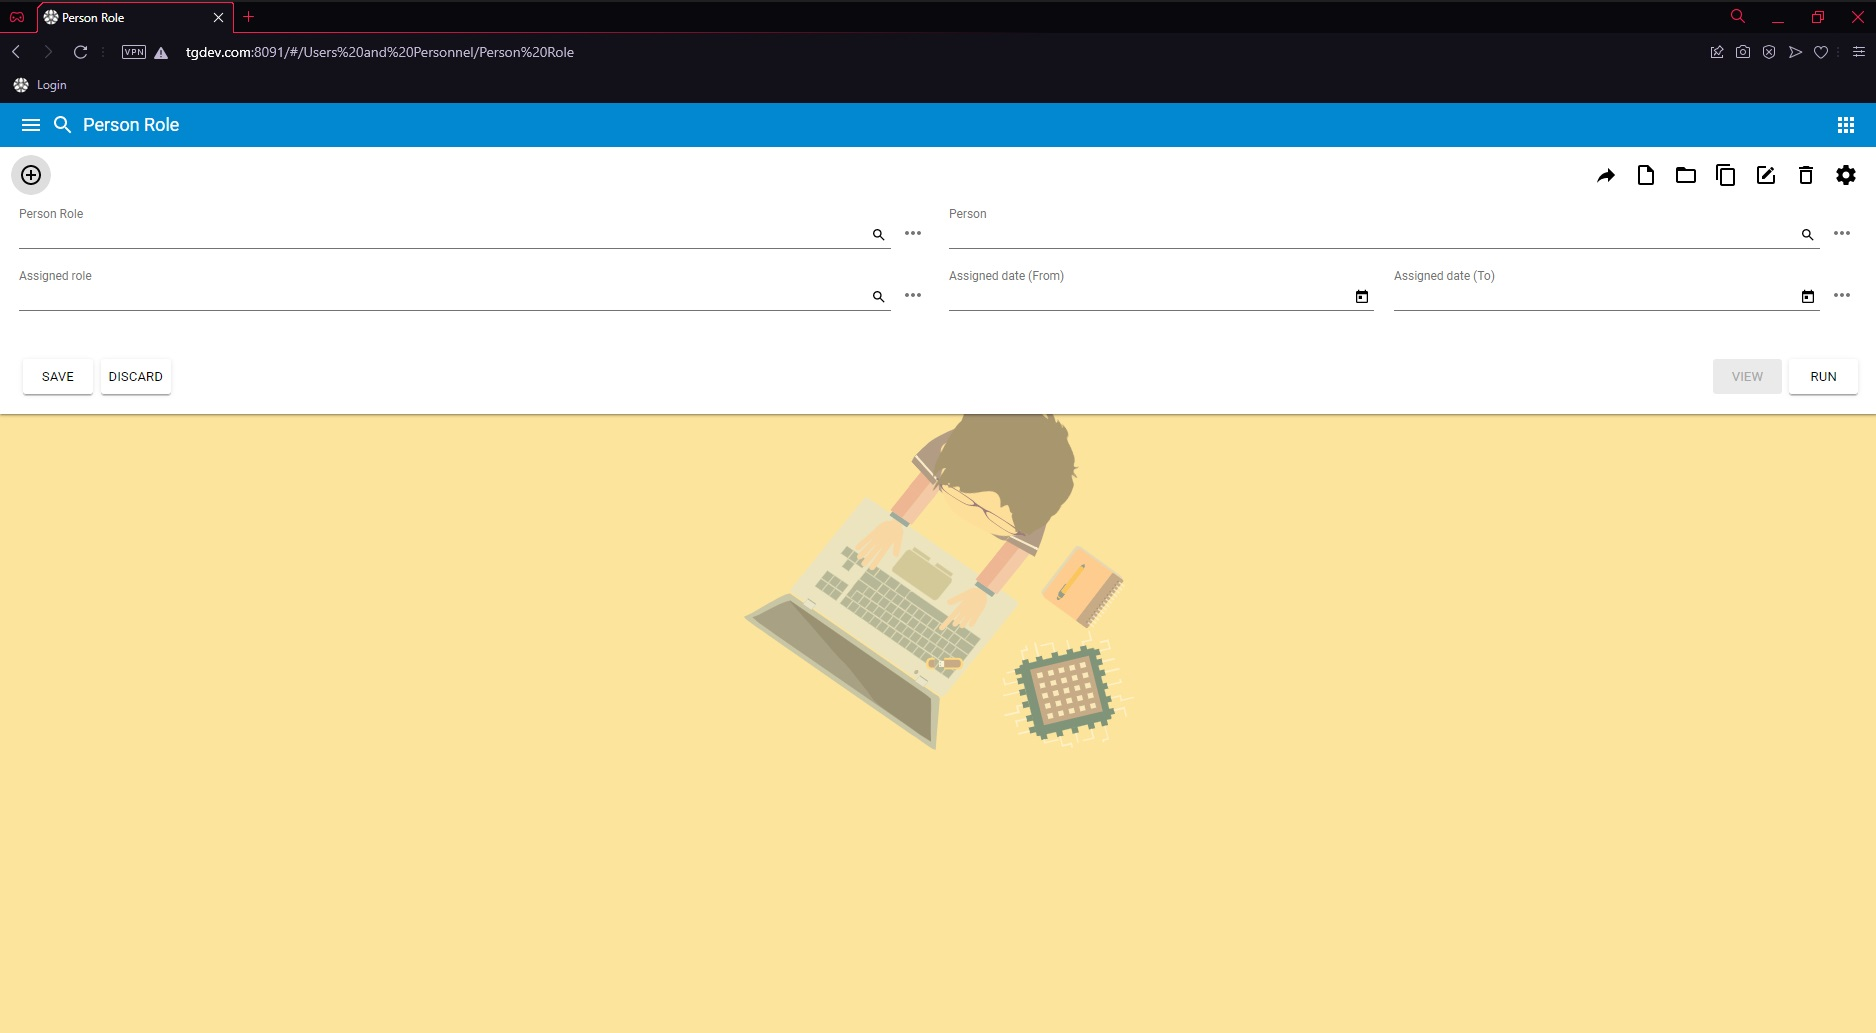
\includegraphics[width=0.95\linewidth]{sections/personnel/images/fig6.jpg}
\caption{Person role search.}\label{sections/personnel/images/fig6}
\end{figure}

\newpage
Users can edit existing person roles. On the ‘Main’ tab, displayed on \hyperref[sections/personnel/images/fig10]{Fig.~\ref*{sections/personnel/images/fig10}}, users can edit the person and role of the specific person role.

\begin{figure}[!htbp]
\centering
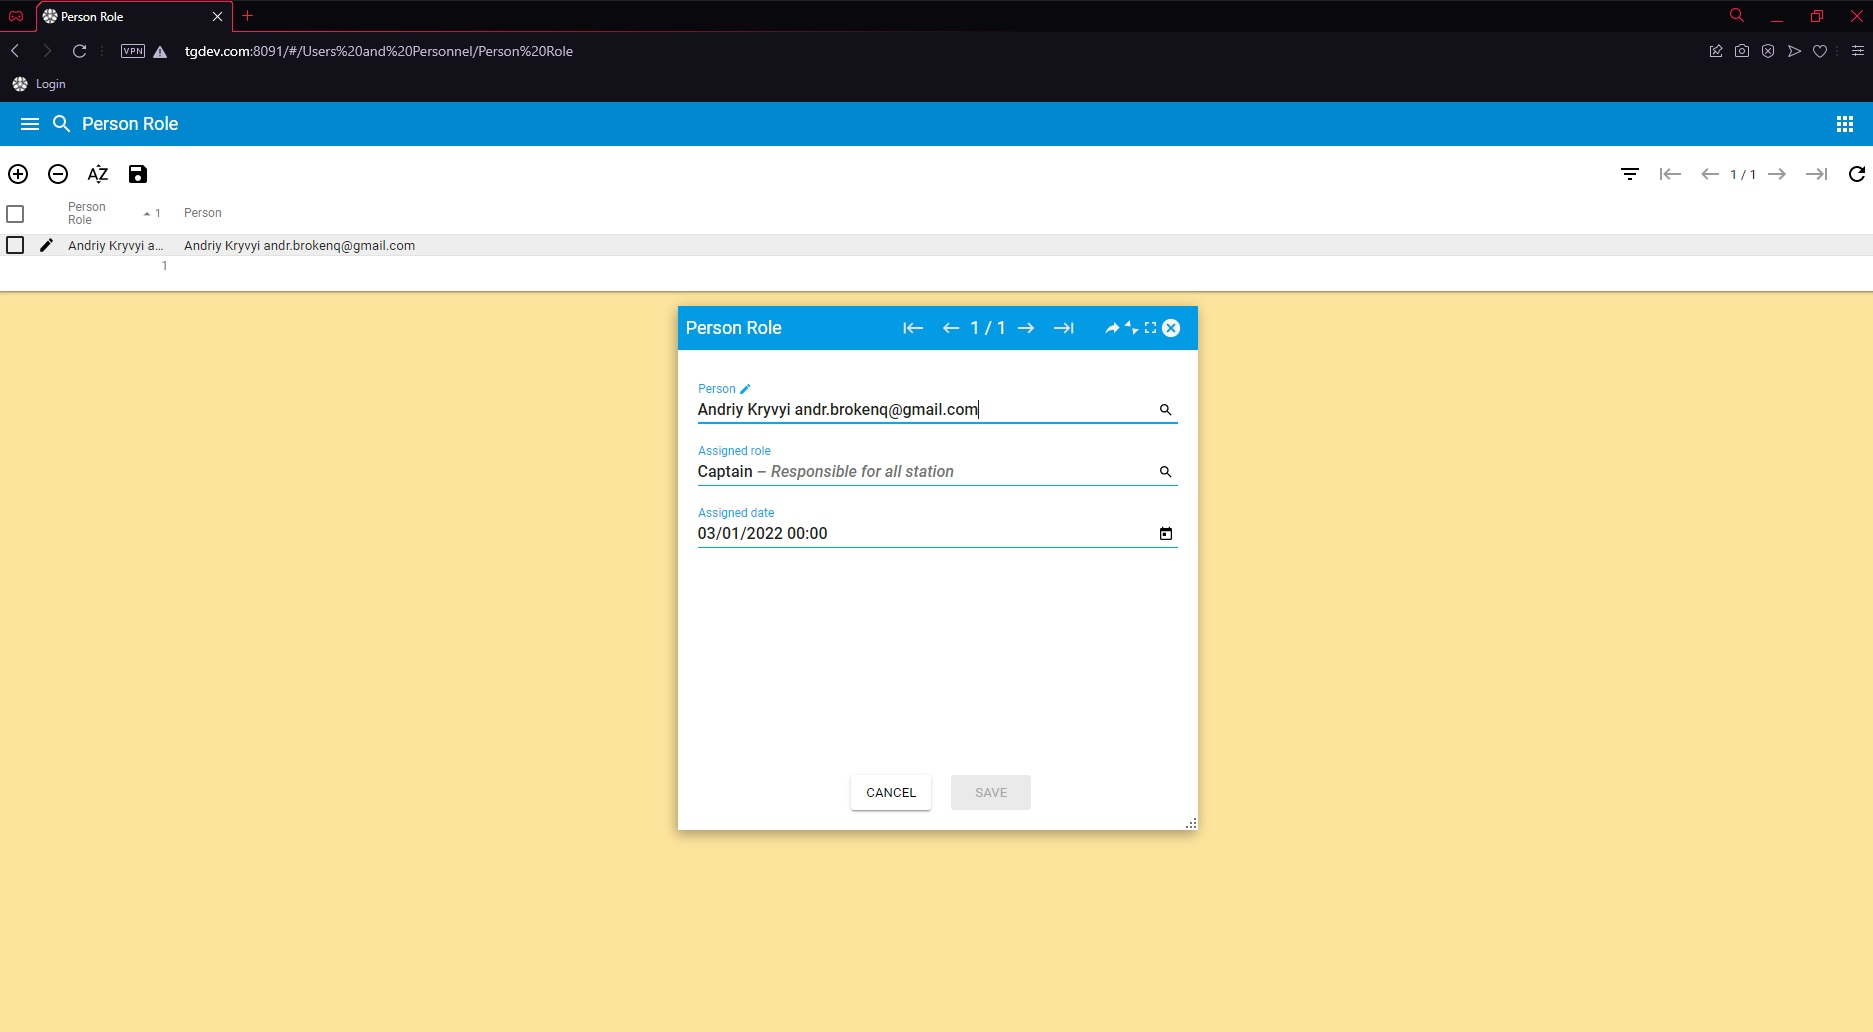
\includegraphics[width=0.95\linewidth]{sections/personnel/images/fig10.jpg}
\caption{Person role editing.}\label{sections/personnel/images/fig10}
\end{figure}


\end{document}

